\documentclass[twoside,a4paper,openright]{report}
\usepackage{astyle}

\newcommand{\nref}{[{\bf REF}]}

% Issue \makeglossaries before defining any entries. *begin.pdf p.12*
%\makeglossaries
%\loadglsentries{tex/glossary}

\begin{document}

% Apply different margins for the title page.
\newgeometry{hmargin=1.5in,vmargin={1.5in,1in}}

\begin{titlepage}

\begin{center}
\setstretch{1.5}


\includegraphics{teia_logo}\\[0.3cm]
\textsc{\LARGE Τεχνολογικό Εκπαιδευτικό Ίδρυμα\\Αθήνασ}\\[2em]

\textsc{\Large Σχολή Τεχνολογικών Εφαρμογών}\\
\textsc{\LARGE Τμήμα Πληροφορικήσ}\\[3em]

\textsc{Πτυχιακή Εργασία}\\[-0.5cm]
{\LARGE\textsf{Μελέτη και υλοποίηση συστήματος αυτοματισμού\\
για την απομακρυσμένη παρακολούθηση περιβαλλοντικών συνθηκών}}\\[1cm]

{\bfseries Θεόδωρος Ελευθέριος \textsc{Πάνου}}\\[-0.1cm]
071045\\[1cm]

Επιβλέπουσα καθηγήτρια\\[-0.1cm]
Ιφιγένεια \textsc{Φουντά}
\\[5cm]

\vfill

\large{Αθήνα, Νοέμβριος 2014}

\end{center}

\end{titlepage}

\cleardoublepage

\thispagestyle{empty}

~\\[5cm]
\begin{center}{\bfseries Ευχαριστίες}

Η καθοδήγηση και η εμψύχωση της επιβλέπουσας καθηγήτριας, καθ' όλη τη διάρκεια
ανάπτυξης της εργασίας, απετέλεσαν καταλύτης για την πραγμάτωση αυτού του
μεγάλου έργου. Τα λόγια αδυνατούν να περιγράψουν επαρκώς τη σπουδαιότητα του
ρόλου τής αξιότιμης κυρίας Ιφιγένειας Φουντά.

Σημαντική ήταν η συμβολή και του κυρίου Αθανάσιου Νασιόπουλου για δύσβατες
πτυχές της εργασίας που ξεφεύγουν από τα πλαίσια της επιστήμης της Πληροφορικής.

Επίσης, ευχαριστώ το προσωπικό του Τμήματος στο σύνολό του καθώς και αυτό έχει
συμβάλει, μέσω των σπουδαστικών ετών, στο τρέχον έργο.
\end{center}

\cleardoublepage

\cleardoublepage

\restoregeometry

\thispagestyle{empty}

\begin{center}{\bfseries Περίληψη}\end{center}

\noindent
Η εργασία ασχολείται με την υλοποίηση μίας συσκευής που αυτοματοποιεί την
παρακολούθηση συνθηκών που επικρατούν στο υλικό ανοικτού δοχείου το οποίο αυτή
περιβάλλει. Η πρόσβαση στη συσκευή πραγματοποιείται απομακρυσμένα με χρήση
πρωτοκόλλου HTTP.
%
Η υλοποίηση στηρίζεται στη χρήση μίας πλακέτας \te{Arduino Uno rev3} και ενός
μικροελεγκτή Atmel AVR ATmega328 που αυτή περιέχει. Ο προγραμματισμός του
μικροελεγκτή γίνεται δια μέσω λογισμικού \te{Boot loader} και διασύνδεσης USB.
Η ανάπτυξη του λογισμικού υποβοηθείται μόνο από την AVR GNU συλλογή
μεταγλωττιστών avr-gcc και τη βιβλιοθήκη προγραμματισμού AVR Libc. Κρίσιμες
δυνατότητες που ο συγκεκριμένος μικροελεγκτής στερείται, όπως ρολόι πραγματικού
χρόνου, δικτυακή διασύνδεση και επιπρόσθετο αποθηκευτικό χώρο, παρέχονται από
εξωτερικά ολοκληρωμένα κυκλώματα.
%
Η συσκευή ρυθμίζεται σε σχέση με παραμέτρους βοηθητικών λειτουργιών της καθώς
και της διαδικασίας παρακολούθησης. Όλες οι ρυθμίσεις διατηρούνται μεταξύ
διακοπών τροφοδοσίας και είναι δυνατό να επαναφερθούν στις εργοστασιακές
της ρυθμίσεις με μηχανικό τρόπο.
%
Για τη διασύνδεσή της με το χρήστη, υλοποιείται λογισμικό διακομιστή HTTP μέσω
του οποίου επιτυγχάνεται η ανάκτηση πόρων, οι οποίοι, σε συνδυασμό με
παρεχόμενες μεθόδους του πρωτοκόλλου HTTP, επιτρέπουν πρόσβαση σε αυτήν.
Η μορφή των αναπαραστάσεων των πόρων γίνεται σε JSON και προορίζεται για
αξιοποίηση από εξωτερικές εφαρμογές. Επιπλέον, υποστηρίζονται πόροι σε HTML,
CSS, JavaScript και PNG για χρήση της συσκευής μέσω λογισμικού πλοήγησης.
%
Το κεντρικό σημείο ενδιαφέροντος της εργασίας έγκειται στην υλοποίηση ενός
ολοκληρωμένου συστήματος που εμπλέκει πληθώρα τεχνολογικών πεδίων.

\clearpage
\thispagestyle{empty}

\begin{center}{\bfseries Abstract}\end{center}

\begin{english}
\noindent
The project's aims is a device that automates monitoring the conditions of the
material within a container. Access to the device is provided remotely via the
HTTP protocol.
%
The core of the implementation is an Arduino Uno rev3 board and an Atmel AVR
ATmega328 microcontroller contained therein. The microcontroller is programmed
via Boot loader software on a USB interface. The development of the firmware is
based solely on the GNU AVR toolchain and AVR Libc library. Important
functionality not inherently present on the microcontroller, such as real-time
clock, network interfacing and additional storage, is provided by external
integrated circuits.
%
The device may be configured as far as monitoring parameters are concerned
as well as supplementary functions it provides. A mechanism is provided so the
configuration is unaffected from power outage, while allowing to manually reset
it to its default factory settings, if needed.
%
The user interface is based on a rudimentary HTTP server; HTTP resources in
combination with HTTP methods provide the fundamental mechanism for remote
access. The resources are represented in JSON format, mostly intended for
external software systems. A few additional resources are provided in HTML, CSS,
JavaScript and PNG intended to be viewed in a web browser.
%
The primary reason for undertaking such a project lies in the desire to
implement a complete system that incorporates various technological fields.
\end{english}

\clearpage


% Use roman numbering in front matter.
\pagenumbering{roman}

\tableofcontents
\listoffigures
\listoftables

\cleardoublepage


% Use arabic numbering for the main matter.
\pagenumbering{arabic}
\setcounter{page}{1}

% Piece together the final document by using the \input command to refer to
% documents from directory tex/.
\chapter{Εισαγωγή}

Η εργασία αναλαμβάνει τη μελέτη, το σχεδιασμό και την υλοποίηση ενός συστήματος
αυτοματισμού με δυνατότητες δικτύωσης.

Το αντικείμενο που επιλέγεται να υποστηριχθεί αντλεί έμπνευση από συστήματα
κομποστοποίησης. Η κομποστοποίηση είναι μία διαδικασία που σκοπό έχει τη
μετατροπή αγροτικών και οικιακών υπολειμμάτων σε πλούσια οργανική μάζα.
Μέσω αυτής, σημειώνονται αρκετά οφέλη για το περιβάλλον και το κοινωνικό σύνολο,
όπως, μείωση όγκου απορριμάτων, εμπλουτισμός εδάφους, ανάληψη ευθύνης απέναντι
στα υποπροϊόντα της ανθρώπινης δραστηριότητας.

Στο πλαίσιο της υλοποίησης επιλέγεται η παρακολούθηση των συνθηκών ενός
υποθετικού δοχείου στο οποίο εναποτίθενται υλικά τα οποία προορίζονται για
αποσύνθεση μέσω ψυχρής κομποστοποίησης που, για την ακρίβεια, κάνει χρήση
γαιοσκώληκα. Σε ένα τέτοιο σύστημα, πρέπει να παρακολουθούνται, κυρίως, η
θερμοκρασία, η υγρασία και η οξύτητα.

Ωστόσο, από τις τρεις αυτές βασικές μεταβλητές, πραγματοποιείται ενδεικτική
υλοποίηση παρακολούθησης μόνο της θερμοκρασίας. Προς επίτευξη αυτού, η συσκευή
διαθέτει ένα ειδικό εξάρτημα που μπορεί να διανύει την επιφάνεια του δοχείου
και να εισχωρεί κατακόρυφα σε αυτό για τη λήψη μετρήσεων.

Τυπικά, η συσκευή ξοδεύει το μεγαλύτερο μέρος της ημέρας σε κατάσταση χαμηλής
κατανάλωσης ισχύος, παρότι συνδεδεμένη στην κεντρική τροφοδοσία. Από αυτήν την
κατάσταση, αφυπνίζεται αυτόματα για την πραγματοποίηση μετρήσεων του υλικού ή
για την απόκριση στις προτροπές του χρήστη.

Σε σχέση με τις αυτόματες μετρήσεις, η συσκευή ρυθμίζεται για τις διαστάσεις του
δοχείου που της προσαρτάται, για το χρονικό διάστημα που είναι επιθυμητό να
παρεμβάλλεται μεταξύ μετρήσεων καθώς και για το πλήθος μετρήσεων που
πραγματοποιούνται κάθε φορά που αφυπνίζεται για το σκοπό αυτό.
Οι θέσεις στις οποίες πραγματοποιούνται μετρήσεις επιλέγονται τυχαία μέσα στο
χώρο του δοχείου, ώστε να παρέχεται μία εικόνα για τη συνολική κατάσταση του
υλικού. Οι 90 πλέον πρόσφατες πραγματοποιηθείσες μετρήσεις αποθηκεύονται σε
μνήμη της συσκευής και φέρουν πληροφορία της ημερομηνίας\slash{}ώρας, της θέσης
και της θερμοκρασίας σε αυτήν.

Η τρέχουσα ημερομηνία\slash{}ώρα καθορίζεται από το χρήστη μία φορά και τηρείται
από κύκλωμά της. Για την ακρίβεια, όλες οι ρυθμίσεις της συσκευής διατηρούνται,
ακόμα και εάν αυτή αποσυνδεθεί από την τροφοδοσία· χαρακτηριστικό ιδιαίτερα
χρήσιμο κατά των διακοπών παροχής ηλεκτρικής ενέργειας.

Μέσα από το λογισμικό περιήγησης της προτίμησής του, δεδομένου ότι αυτό
υποστηρίζει στοιχειωδώς HTML5, CSS3 και Javascript (ΙΕ8/2006 και μετά), από
οποιασδήποτε μορφής υπολογιστή που έχει πρόσβαση στο δίκτυο της συσκευής, ο
χρήστης μπορεί να ενημερώνεται για τις τελευταίες μετρήσεις, να εκτελεί κατά
παραγγελία μετρήσεις στις θέσεις που επιθυμεί και, σαφώς, να τροποποιεί τις
ρυθμίσεις της συσκευής.

Παρότι η σύνδεση του χρήστη με τη συσκευή γίνεται από μία προκαθορισμένη
διεύθυνση, επιτρέπεται η αλλαγή αυτής καθώς και των υπόλοιπων ρυθμίσεων δικτύου,
ώστε να διευκολύνεται η πρόσβαση σε αυτήν μέσα από το τοπικό δίκτυο του εκάστοτε
χρήστη. Ωστόσο, σε περίπτωση που οι ρυθμίσεις αυτές απολεσθούν (κυρίως της
διεύθυνσης IP) με αποτέλεσμα να μην δύναται η πρόσβαση στη διεπαφή της συσκευής,
παρέχεται η δυνατότητα επαναφοράς της συσκευής στις εργοστασιακές της ρυθμίσεις.
Αυτό επιτυγχάνεται με την προσωρινή απομάκρυνση μίας μικρής \te{coin cell}
μπαταρίας που διαθέτει κατά το διάστημα που βρίσκεται απενεργοποιημένη (καλώδιο
τροφοδοσίας αποσυνδεδεμένο).

Ο πιο προχωρημένος χρήστης έχει στη διάθεσή του ένα εύχρηστο προγραμματιστικό
API, το οποίο του επιτρέπει να χειρίζεται τη συσκευή μέσω δικών του εφαρμογών.
Όλη η λειτουργικότητα που παρέχεται μέσω της διεπαφής που προορίζεται για
λογισμικό πλοήγησης, παρέχεται και μέσω του API -- για την ακρίβεια, η διεπαφή
αποτελεί μία τέτοια εφαρμογή που κάνει χρήση αυτού του API.

Το API χρησιμοποιεί την μορφή JSON για την αναπαράσταση των πόρων και
υλοποιείται με την ανταλλαγή μηνυμάτων HTTP και καθιερωμένων μεθόδων (GET, PUT,
POST), ενώ διαγνωστικά μηνύματα, όπως «Το αίτημα μετακίνησης της κεφαλής έγινε
αποδεκτό· αναμενόμενος χρόνος ολοκλήρωσης 7s», επιστρέφονται με τη μορφή
κατάλληλων κωδικών κατάστασης και πεδίων επικεφαλίδας του πρωτοκόλλου HTTP (στο
παράδειγμα, 202 και «Retry-After», αντίστοιχα). Οδηγίες χρήσης παρέχονται μέσα
από τη διεπαφή της συσκευής.

\chapter{Περιγραφή υλοποίησης}


\section{Περιβάλλον ανάπτυξης}

Η επιλογή μικροελεγκτή (MCU) αντί μικροεπεξεργαστή (MPU) για την ανάληψη των
καθηκόντων της υλοποίησης θεωρείται δεδομένη.
Ως βασικά στοιχεία υπεροχής των μικροελεγκτών κρίνεται η χαμηλότερη κατανάλωση
ισχύος, η έλλειψη ανάγκης σύνδεσης και τροφοδοσίας εξωτερικής κύριας και
δευτερεύουσας μνήμης, και ο λιγότερος (φυσικός) χώρος που καταλαμβάνουν
\parencite[1--2]{atmel13:mpu-mcu}. Αυτά βέβαια παρέχονται εις βάρος χαμηλότερης
επεξεργαστικής ισχύος και λιγότερης μνήμης που, σε αντίθεση με τους
μικροεπεξεργαστές που υποστηρίζουν μεγέθη της τάξης των GiB, οι μικροελεγκτές
περιορίζονται σε μερικά MiB.

Βέβαια, παρότι ένας μικροελεγκτής είναι πιο συμπαγής, απαιτούνται, τελικά,
ορισμένα επιπρόσθετα στοιχεία όπως, για παράδειγμα, για τη ρύθμιση και
σταθεροποίηση της τάσης που αυτός λαμβάνει. Επιπλέον, τίθενται ζητήματα που
αφορούν τον προγραμματισμού του καθώς και τη (φυσική) διασύνδεση με τα
οποιαδήποτε εξαρτήματα και εξωτερικά ολοκληρωμένα που πρόκειται να
χρησιμοποιηθούν.


\subsection{Πλατφόρμα Arduino}
\label{subsec:arduino}

Οι πλακέτες Arduino επιλύουν τα παραπάνω ζητήματα και παρέχουν μία έτοιμη
λειτουργική μονάδα που επιτρέπει την άμεση ενασχόληση με τη δημιουργία του
πρότυπου λογισμικού και εκείνων των συνδέσεων με ηλεκτρονικά στοιχεία που
απαιτούνται στο πλαίσιο αυτού.

Για την ύπαρξη αρκετής ευελιξίας κατά το σχεδιασμό της υλοποίησης (και λόγω
έλλειψης πρότερης εμπειρίας και, επομένως, κρίσης), επιλέγεται η (πλέον
πρόσφατη, την περίοδο εκπόνησης) πλακέτα Arduino Uno revision 3, της οποίας ο
κεντρικός μικροελεγκτής είναι ένας AVR ATmega328P της Atmel. Ο συγκεκριμένος
μικροελεγκτής διαθέτει συνολική μνήμη προγράμματος 32KiB, 2KiB κύρια μνήμη,
συχνότητα ρολογιού που φτάνει τα 20MHz (που, ωστόσο, λόγω της πλακέτας,
περιορίζεται στα 16MHz) και πληθώρα δυνατοτήτων
\parencites[1]{atmel13}{arduino:uno}. Επιπροσθέτως, η πλακέτα παρέχει διασύνδεση
USB για την επικοινωνία του μικροελεγκτή με τον υπολογιστή, τόσο για τον
προγραμματισμό του όσο και για την ανταλλαγή δεδομένων με κάποια άλλη εφαρμογή,
για παράδειγμα τερματικό. Στο σχήμα \ref{fig:arduino:uno-front} παρουσιάζεται η
πλακέτα Arduino και τα βασικά της μέρη.

\begin{figure}
    \caption{Πλακέτα Arduino Uno.\label{fig:arduino:uno-front}}
    \begin{center}
    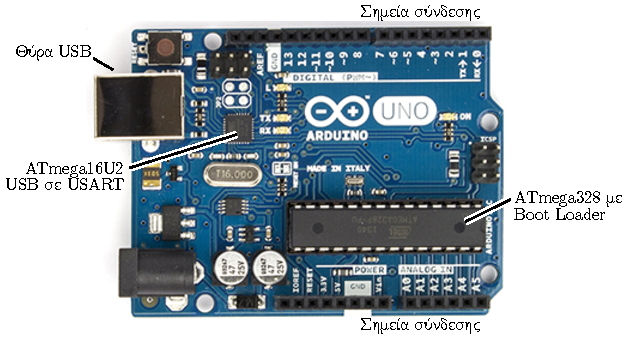
\includegraphics{arduino_uno}
    \end{center}
    Βασισμένο. \fullcite{arduino:uno:front}
\end{figure}

Ο μικροελεγκτής της πλακέτας \te{Arduino Uno revision 3} διατίθεται με
προεγκατεστημένο
λογισμικό \te{Boot loader} επιτρέποντας, με αυτόν τον τρόπο, τον προγραμματισμό
της μνήμης προγράμματος χωρίς τη χρήση ειδικού υλικού, αλλά με την απευθείας
σύνδεση της πλακέτα μέσω καλωδίου USB \parencite{arduino:environ}. Περισσότερα
σχετικά με το λογισμικό \te{Boot loader} αναφέρονται στην ενότητα
\nameref{subsec:avr:progmem} σ.~\pageref{subsec:avr:progmem}.
Ωστόσο, σημειώνεται ότι η
επικοινωνία μέσω USB επιτυγχάνεται με ένα δεύτερο μικροελεγκτή της πλακέτας --
ενός ATmega16U2 -- του οποίου μοναδικός σκοπός είναι η διασύνδεση του
πρωτοκόλλου USB (το οποίο υποστηρίζει εγγενώς) με το κύκλωμα USART που διαθέτει,
τόσο ο ίδιος, αλλά, κυρίως, ο ATmega328P -- ο κεντρικός μικροελεγκτής της
πλακέτας \parencites{arduino:uno}[148,185]{atmel12}[172]{atmel13}. Σαφώς, αυτή η
διασύνδεση χρησιμοποιείται για κάθε επικοινωνία μεταξύ υπολογιστή και πλακέτας
μέσω καλωδίου USB, ανεξαρτήτως εάν τα δεδομένα προορίζονται για το λογισμικό
\te{Boot loader} ή το ίδιο το πρόγραμμα.

Για την περαιτέρω διευκόλυνση της ανάπτυξης του λογισμικού του μικροελεγκτή της
πλακέτας,
παρέχεται ορισμένο επιπρόσθετο λογισμικό \te{Arduino} το οποίο λαμβάνει δύο
μορφές. Μία εξ αυτών είναι το περιβάλλον ανάπτυξης \te{Arduino IDE} του οποίου
οι βασικές λειτουργίες είναι η μεταγλώττιση του πηγαίου κώδικα και η μεταφορά
του προγράμματος στο μικροελεγκτή \parencite{arduino:environ} μέσω μίας
περισσότερο ελκυστικής γραφικής διεπαφής. Μία δεύτερη μορφή
λογισμικού είναι οι βιβλιοθήκες \te{Arduino} οι οποίες παρέχουν εύχρηστες
προγραμματιστικές διεπαφές (API) που εσωτερικά κάνουν χρήση των υποκείμενων
κυκλωμάτων του μικροελεγκτή της εκάστοτε πλακέτας (είτε απευθείας, είτε μέσω
τρίτου λογισμικού) αποκρύπτοντας, με αυτόν τον τρόπο, τις λεπτομέρειες της
υλοποίησης \parencite{arduino:lib}.


\subsubsection{Εργαλεία προγραμματισμού}
\label{subsubsec:avr:toolchain}

Παρότι το IDE και οι βιβλιοθήκες Arduino μπορούν να επιταχύνουν σημαντικά τη
διαδικασία ανάπτυξης της υλοποίησης, προτιμάται, αντί αυτών, η απευθείας χρήση
καθιερωμένων εργαλείων για τον προγραμματισμό μικροελεγκτών AVR, καθώς έτσι
επιδιώκεται να επιτευχθεί σε μεγαλύτερο βάθος κατανόηση της συνολικής
διαδικασίας που, ιδανικά, θα επιτρέψει τη μελλοντική ενασχόληση με παρόμοια
συστήματα ανεξαρτήτως της πορείας των προϊόντων \te{Arduino}. Στο πλαίσιο της
υλοποίησης, χρησιμοποιείται μόνο το υλικό, δηλαδή η πλακέτα \te{Arduino} για την
κάλυψη των βασικών ηλεκτρικών αναγκών, και το λογισμικό \te{Boot loader} για τον
προγραμματισμό του μικροελεγκτή καθώς και το λογισμικό του ATmega16U2 το οποίο
διασυνδέει τον κεντρικό μικροελεγκτή με τη θύρα USB.

Το IDE αντικαθίσταται από έναν οποιοδήποτε επεξεργαστή κειμένου και ο πηγαίος
κώδικας διασπάται σε διαφορετικά αρχεία για την καλύτερη οργάνωσή του.
Με τον τρόπο αυτό, καθώς η υλοποίηση επεκτείνεται και ο κώδικάς της διογκώνεται,
ο λογικός διαχωρισμός των λειτουργιών της επιτρέπει το γρηγορότερο εντοπισμό
κάποιας συγκεκριμένης υπομονάδας. Επιπλέον, καθώς η μεταγλώττιση μεγάλου όγκου
πηγαίου κώδικα μπορεί να αποβεί χρονοβόρα, η ύπαρξη αυτόνομων αρχείων
αντικείμενου προγράμματος δημιουργημένων από προηγούμενο κύκλο μεταγλώττισης,
επιτρέπει την επαναχρησιμοποίησή τους για την παραγωγή ενός (νέου) συνολικού
δυαδικού αρχείου, απαιτώντας μεταγλώττιση μόνο των αρχείων εκείνων που έχουν
τροποποιηθεί.

Η μεταγλώττιση των επιμέρους αρχείων πηγαίου κώδικα σε αντικείμενα προγράμματα
και η, εν συνεχεία, σύνδεση (ή συνένωσή) τους σε ένα τελικό δυαδικό αρχείο
αναλαμβάνεται από την AVR GNU συλλογή μεταγλωττιστών avr-gcc και λοιπών
εργαλείων της avr-binutils (όπως ο συνδέτης ld ο οποίος χρησιμοποιείται
εσωτερικά από την avr-gcc). Η σύνταξη του κώδικα γίνεται σε γλώσσα C με τη
βοήθεια της βιβλιοθήκης AVR Libc.

Το παραγόμενο δυαδικό αρχείο της σύνδεσης είναι μορφής ELF (\te{Executable and
Linking Format}) η οποία, παρότι παρέχει ανεξαρτησία από επεξεργαστή και
αρχιτεκτονική υπολογιστή, είναι, ωστόσο ακατάλληλη για την απευθείας μεταφορά
στο μικροελεγκτή AVR \parencites[47]{cruz97}[346]{avrlibc}. Απαιτείται, πρώτα, η
εξαγωγή των τμημάτων (\te{segment}) του κώδικα και των δεδομένων (\@.\te{text}
και \@.\te{data}, αντίστοιχα) από το αρχείο ELF σε ένα αρχείο δεκαεξαδικής
μορφής (αρχείο HEX) · εργασία η οποία αναλαμβάνεται από το εργαλείο avr-objcopy
\parencite[13,346]{avrlibc}.

\begin{figure}
    \caption{Η αλυσίδα εργαλείων AVR GCC για τον προγραμματισμό του
    μικροελεγκτή.\label{fig:avr:toolchain}}
    \begin{center}
    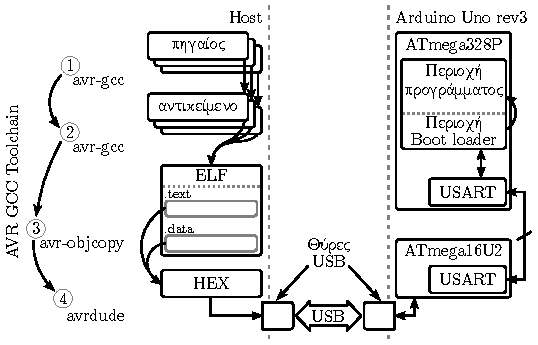
\includegraphics{avr_toolchain}
    \end{center}
\end{figure}

Τέλος, το δεκαεξαδικό αρχείο περνάει στο μικροελεγκτή μέσω του εργαλείου
avrdude, το
οποίο υποστηρίζει προγραμματισμό μικροελεγκτών AVR μέσω διαφόρων προγραμματιστών
(συμπεριλαμβανομένου ειδικών εξαρτημάτων όπως οι STK500 και AVRISP mkII της
Atmel) και, σαφώς, μέσω \te{Boot loader} \parencites[15]{avrlibc}{avrdude}.

Σημειώνεται ότι, γενικά, η χρήση \te{Boot loader} περιορίζεται στην εγγραφή και
ανάγνωση της μνήμης \te{Flash} και EEPROM χωρίς να παρέχεται η δυνατότητα
εγγραφής των λεγόμενων \te{fuse bit}, τα οποία πρόκειται για μη πτητικές θέσεις
μνήμης που ρυθμίζουν, με διάφορους τρόπους, τη συμπεριφορά του μικροελεγκτή
όπως, για παράδειγμα, το μέγεθος της περιοχής \te{Boot loader} (σχετικά με
αυτήν, βλ. \nameref{subsec:avr:progmem} σ.~\pageref{subsec:avr:progmem})· κάτι
τέτοιο είναι δυνατό μόνο μέσω σειριακών ή παράλληλων συνδέσεων προγραμματισμού
\parencite[273]{atmel13}.  Επιπλέον, στην περίπτωση του \te{Boot loader} του
Arduino Uno revision 3, παρέχεται εγγραφή αποκλειστικά και μόνο για τη μνήμη
προγράμματος (μνήμη \te{Flash}), κυρίως για τη μείωση του μεγέθους του.


\subsubsection{Εντολές προγραμματισμού}

Στο σχήμα \ref{fig:avr:toolchain} παρουσιάζεται η αλυσίδα (\te{toolchain}) των
χρησιμοποιούμενων εργαλείων για τη μετάβαση από κάθε στάδιο στο επόμενο με
τελικό στόχο τον προγραμματισμό του μικροελεγκτή. Στη βασική τους μορφή, οι
εντολές συνοψίζονται παρακάτω.

\begin{enumerate}

    \item Μετατροπή αρχείων πηγαίου σε αρχεία αντικείμενου προγράμματος για κάθε
    αρχείο \verb~file.c~. Τυπικά, η εντολή εκτελείται μόνο για εκείνα τα αρχεία
    πηγαίου κώδικα που έχουν τροποποιηθεί.

\begin{lstlisting}
avr-gcc -mmcu=atmega328 -Wl,-Map,mcu.map -Os -c file.c
\end{lstlisting}

    \begin{description}
        \item[-mmcu] Καθορίζει τον τύπο του μικροελεγκτή ώστε να αναγνωρίζεται
        το κατάλληλο σύνολο εντολών (\te{instruction set}) που πρόκειται να
        χρησιμοποιηθεί κατά τη συμβολομετάφραση \parencite{gcc:options}.

        \item[-Os] Ενεργοποιεί τις βελτιστοποιήσεις του κώδικα από το
        μεταγλωττιστή προκειμένου να εξοικονομηθεί χώρος προγράμματος, ακόμα και
        εις βάρος της ταχύτητας εκτέλεσής του (Optimize for size)
        \parencites[338]{avrlibc}{gcc:options}.

        Εκτός του άμεσου πλεονεκτήματος της παραγωγής μικρότερου προγράμματος, η
        συγκεκριμένη ρύθμιση απαιτείται από τη βιβλιοθήκη AVR Libc προκειμένου
        να διατίθενται ορισμένες λειτουργίες προσωρινής «παύσης» της εκτέλεσης
        του προγράμματος (βρόχοι \te{busy-wait}) \parencite[328]{avrlibc}.

        \item[-c] Η συγκεκριμένη επιλογή προκαλεί την παραγωγή αρχείου
        αντικείμενου προγράμματος όπως αυτό εξάγεται από το συμβολομεταφραστή,
        αποτρέποντας τη σύνδεσή του σε τελικό πρόγραμμα
        \parencites[338]{avrlibc}{gcc:options}.
    \end{description}


    \item Σύνδεση των αρχείων αντικείμενου προγράμματος σε αρχείο ELF.
\begin{lstlisting}
avr-gcc -mmcu=atmega328 *.o -o mcu.elf
\end{lstlisting}

    \begin{description}
        \item[-mmcu] Ομοίως με την προηγούμενη εντολή.

        \item[-o] Καθορίζει το όνομα του παραγόμενου αρχείου
        \parencite{gcc:options}.
    \end{description}


    \item Μετατροπή αρχείου ELF σε δεκαεξαδική μορφή Intel HEX.
\begin{lstlisting}
avr-objcopy -j .text -j .data -O ihex mcu.elf mcu.hex
\end{lstlisting}

    \begin{description}
        \item[-j] Καθορίζει ποια τμήματα του αρχείου ELF θα χρησιμοποιηθούν για
        τη δημιουργία του αρχείου εξόδου. Στην προκειμένη, εξάγεται ο κώδικας
        και τα δεδομένα \parencite[346]{avrlibc}.

        \item[-O] Καθορίζει τον τύπο του παραγόμενου αρχείου
        \parencite[346]{avrlibc}. Στην περίπτωση του μικροελεγκτή AVR, πρόκειται
        για ένα αρχείο κειμένου ASCII του οποίου τα δεκαεξαδικά ψηφία
        κωδικοποιούν, ένα προς ένα, τα Byte του αρχικού δυαδικού αρχείου το
        οποίο αποτελεί το πρόγραμμα που εγγράφεται στη μνήμη Flash
        \parencites[4]{intel88}[10]{atmel12programmer}.
    \end{description}


    \item Αποστολή αρχείου HEX στο λογισμικό \te{Boot loader} του μικροελεγκτή
    για τη μετέπειτα εγγραφή του στην περιοχή προγράμματος (βλ.
    \nameref{subsec:avr:progmem} σ.~\pageref{subsec:avr:progmem}).
\begin{lstlisting}
avrdude -p atmega328p -c arduino -P /dev/ttyACM0 -b 115200 -U flash:w:mcu.hex:i
\end{lstlisting}
    \begin{description}
        \item[-p] Το μοντέλο του μικροελεγκτή, το οποίο στην περίπτωση της
        υλοποίησης είναι ο ATmega328P.

        \item[-c] Ο χρησιμοποιούμενος προγραμματιστής, ώστε να αναγνωρίζεται η
        συνδεσμολογία με το μικροελεγκτή και να εφαρμόζονται τα κατάλληλα
        σήματα ελέγχου.

        \item[-P] Η θύρα του υπολογιστή στην οποία είναι συνδεδεμένος ο
        προγραμματιστής. Στην περίπτωση της υλοποίησης όπου χρησιμοποιείται
        \te{Boot loader}, η θύρα σύνδεσης είναι USB η οποία, στο σύστημα του
        υπολογιστή, εμφανίζεται ως \slash{}dev\slash{}ttyACM0.

        \item[-b] Ο ρυθμός baud μετάδοσης δεδομένων μέσω της σειριακής. Σύμφωνα
        με τις προδιαγραφές του Arduino Uno, ο χρησιμοποιούμενος \te{Boot
        loader} λειτουργεί στα 115200Bd \parencite{arduino:environ}.

        \item[-U] Ο τύπος της εργασίας που πρόκειται να εκτελεστεί. Το πρόγραμμα
        avrdude μπορεί να χρησιμοποιηθεί τόσο για την εγγραφή όσο και για την
        ανάγνωση των διαθέσιμων μνημών του εκάστοτε μικροελεγκτή (για
        παράδειγμα, \te{Flash}, EEPROM, \te{fuse}), εφόσον αυτό υποστηρίζεται%
        \slash{}επιτρέπεται από τον μικροελεγκτή \parencite{avrdude}. Στο
        πλαίσιο της υλοποίησης, ενδιαφέρει μόνο η εγγραφή (\verb~w~) της μνήμης
        \te{Flash} με τα δεδομένα του αρχείου HEX (μορφής \verb~i~ntel).
    \end{description}

\end{enumerate}


\subsection{Λοιπό λογισμικό ανάπτυξης}

Πέραν των εργαλείων της συλλογής AVR GCC που περιγράφονται στην ενότητα
\nameref{subsubsec:avr:toolchain} (σ.~\pageref{subsubsec:avr:toolchain}),
χρησιμοποιούνται και ορισμένα άλλα. Όλα πρόκειται για Ελεύθερο λογισμικό αδείας
συμβατής είτε με την άδεια GNU GPL είτε την LGPL, με τα περισσότερα να
υποστηρίζουν πολλαπλά λειτουργικά συστήματα πέραν των βασισμένων σε \te{UNIX}.

\begin{description}

\item[Make]
Εργαλείο αυτοματισμού της ενημέρωσης παρακολουθούμενων αρχείων, αναγνωρίζει,
βάσει κανόνων που του δηλώνει ο χρήστης, ποια αρχεία έχουν τροποποιηθεί και
ενεργοποιεί τις αντίστοιχες εντολές για την ενημέρωσή αυτών καθώς και πιθανών
άλλων αρχείων εξαρτώμενων από αυτών που μόλις ενημερώθηκαν
\parencite{make:intro}.

Στο πλαίσιο της
υλοποίησης, χρησιμοποιείται για την εκ νέου μεταγλώττιση μόνο εκείνων των
αρχείων πηγαίου κώδικα που έχουν τροποποιηθεί, παράγοντας τα αντίστοιχα αρχεία
αντικείμενου προγράμματος και την, εν συνεχεία, σύνδεσή τους για την παραγωγής
του αρχείου HEX. Επίσης, περιλαμβάνει τη μεταφορά του αρχείου στο μικροελεγκτή
καθώς και τη σύνταξη της τεκμηρίωσης (βλ. επόμενο εργαλείο).


\item[\LaTeX]
Σύστημα προετοιμασίας εγγράφων υψηλής τυπογραφικής αξίας, ορίζει ειδική σήμανση
κειμένου που χρησιμοποιείται για το χαρακτηρισμό του κειμένου και μέσω ορισμένων
εργαλείων, παράγεται το τελικό έγγραφο \parencite{latex}. Η παρουσίαση\slash{}%
εμφάνιση του εγγράφου (όπως περιθώρια, διατάξεις) καθορίζεται από,
τροποποιήσιμους έως ένα βαθμό, προκαθορισμένους εσωτερικούς κανόνες του
συστήματος \LaTeX{}  που έχουν δημιουργηθεί ώστε να ευνοείται η αναγνωσιμότητα
του τελικού προϊόντος.

Το σύστημα \LaTeX και τα σχετικά εργαλεία χρησιμοποιούνται για τη σύνταξη της
τεκμηρίωσης (του παρόντος εγγράφου). Μεταξύ άλλων, διευκολύνεται η εργασία με
αναφορές, τόσο μεταξύ μερών του εγγράφου όσο και των βιβλιογραφικών αναφορών και
η διατύπωση μαθηματικών παραστάσεων. Επίσης, καθώς ο επεξεργαστής κειμένου είναι
υπεύθυνος για την εμφάνιση μόνο κειμένου, η απόκριση του είναι ταχύτερη και ο
χειρισμός του πιο αποτελεσματικός.

Τέλος, επειδή τα αρχεία είναι κειμένου και όχι δυαδικά, οι αλλαγές που
πραγματοποιούνται σε αυτά είναι δυνατό να παρακολουθούνται από το σύστημα
παρακολούθησης αλλαγών σε επίπεδο γραμμής (βλ. επόμενο εργαλείο).

\item[Git]
Σύστημα παρακολούθησης αλλαγών το οποίο χαρακτηρίζεται για την ταχύτητα
τη μικρή επιβάρυνση σε πόρους συστήματος και την ευελιξία του \parencite{git}.
Επιτρέπει, μεταξύ άλλων, την καταγραφή των αλλαγών που πραγματοποιούνται σε
αρχεία της υλοποίησης (κατά κύριο λόγο, του πηγαίου κώδικα υλοποίησης και
τεκμηρίωσης) και παρέχει τη δυνατότητα πραγματοποίησης εύκολα αναστρέψιμων
πειραματικών αλλαγών.
Επιπλέον, παρέχει μία εύληπτη παρουσίαση πορείας των εργασιών που έχουν
πραγματοποιηθεί.

\item[Doxygen]
Λογισμικό παραγωγής τεκμηρίωσης πηγαίου κώδικα μέσω ειδικών σημάνσεων που
εισάγονται στα σχόλιά του, κυρίως απευθυνόμενο σε κώδικα γλώσσας C και C++
\parencite{doxygen}. Το σύνολο του πηγαίου κώδικα της υλοποίησης (για
παράδειγμα, συναρτήσεις, δομές, μεταβλητές) τεκμηριώνεται σύμφωνα με τις οδηγίες
του \te{Doxygen} ώστε να είναι δυνατή η δημιουργία ενός, ηλεκτρονικής μορφής,
προγραμματιστικού εγχειριδίου των επιμέρους μονάδων (\te{module}) για την
υποστήριξη της κατανόησης της λειτουργίας του καθενός και τη διευκόλυνση της
ενσωμάτωσης τους σε πιθανές άλλες υλοποιήσεις.

\item[Qucs]
Λογισμικό με γραφικό περιβάλλον (GUI) για τη δημιουργία και προσομοίωση
κυκλωμάτων, με δυνατότητα απεικόνισης των αποτελεσμάτων των προσομοιώσεων σε
διάφορες μορφές, όπως γραφήματα \parencite{qucs}.
Χρησιμοποιείται για το σχεδιασμό του προτύπου της διασύνδεσης του μικροελεγκτή
με όλα τα ολοκληρωμένα κυκλώματα και τα συμπληρωματικά στοιχεία της υλοποίησης.
Επιλέγεται, κυρίως, λόγω της ευκολίας με την οποία δημιουργούνται προσαρμοσμένα
κυκλώματα και επειδή υποστηρίζει την εξαγωγή των κυκλωμάτων σε διανυσματική
μορφή που εύκολα ενσωματώνεται στο έγγραφο της τεκμηρίωσης, δίχως απώλειες στην
ποιότητά τους.

\item[Inkscape]
Λογισμικό σχεδίασης διανυσματικών γραφικών \parencite{inkscape}. Χρησιμοποιείται
για τη δημιουργία όλων των επεξηγηματικών σχημάτων της τεκμηρίωσης για το λόγο
ότι επιτρέπει γρήγορη σχεδίαση γραφικών υψηλής ευκρίνειας με δυνατότητα εύκολης
ενσωμάτωσης στην τεκμηρίωση.

\item[Blender3D]
Ολοκληρωμένη σουίτα δημιουργίας τρισδιάστατων γραφικών \parencite{blender3d}.
Στο πλαίσιο της υλοποίησης, χρησιμοποιείται στο κομμάτι της κατασκευής της
συσκευής, τόσο για το σχεδιασμό και εξέταση προτύπων όσο και για την εξαγωγή
απεικονίσεων του εφαρμοσμένου προτύπου που περιλαμβάνονται, κυρίως, στο κεφάλαιο
\nameref{ch:construction} (σ.~\pageref{ch:construction}).

\item[Gimp]
Λογισμικό επεξεργασίας εικόνας \parencite{gimp}. Χρησιμοποιείται για τη βελτίωση
των χαρακτηριστικών ορισμένων εικόνων (για παράδειγμα, αντίθεση, κορεσμός), ώστε
να παρέχεται καλύτερο οπτικό αποτέλεσμα.
\end{description}


\section{Μικροελεγκτής}

Σύμφωνα με τον \textcite[1]{myklebust97}, οι μικροελεγκτές AVR διαθέτουν
μειωμένο σύνολο εντολών, δηλαδή είναι υπολογιστές RISC (\te{Reduced Instruction
Set Computer}). Το χαρακτηριστικό αυτό απλοποιεί τα απαιτούμενα κυκλώματα
ελέγχου και τους παρέχουν μικρότερους κύκλους για την εκτέλεση κάθε εντολής
\parencite[1]{sequin82}. Επιπροσθέτως, οι μικροελεγκτές AVR βασίζονται σε
τροποποιημένη αρχιτεκτονική Harvard σύμφωνα με την οποία, και σε αντίθεση με την
κατά Von Neumann αρχιτεκτονική, το πρόγραμμα και τα δεδομένα τοποθετούνται σε
ανεξάρτητα φυσικά μέσα που χαρακτηρίζονται, μεταξύ άλλων, από ανεξάρτητους
διαύλους πρόσβασης \parencite[1]{myklebust97}.

Άμεσα πλεονεκτήματα αυτού του σχεδιασμού είναι ότι καθίσταται δυνατή η
ταυτόχρονη πρόσβαση στις μνήμες προγράμματος και δεδομένων στον ίδιο κύκλο
\parencite[8]{atmel13}. Επιπλέον, επιτρέπεται η χρήση διαφορετικών τεχνολογιών
για κάθε μνήμη. Για παράδειγμα, στην περίπτωση του χρησιμοποιούμενου
μικροελεγκτή, ATmega328P, τα δεδομένα οργανώνονται σε μνήμη πλάτους των 8bit
τεχνολογίας SRAM (\te{Static RAM}) με 2KiB συνολική χωρητικότητα, ενώ οι
εντολές, σε μνήμη Flash των 32KiB με θέσεις των 16bit
\parencite[8--9,16,18]{atmel13}.


\subsection{Μνήμη προγράμματος}
\label{subsec:avr:progmem}

Η μνήμη Flash του μικροελεγκτή χωρίζεται σε δύο περιοχές λογισμικού, την περιοχή
του προγράμματος (\te{Application section}) και την περιοχή του λογισμικού
\te{Boot loader} (\te{Boot Loader Section} -- BLS) \parencite[269]{atmel13}.
Η περιοχή προγράμματος φέρει τον κώδικα που εκτελεί ο μικροελεγκτής κατά την
τυπική του λειτουργία· τον κώδικα της υλοποίησης. Στην περιοχή BLS εναποτίθεται
λογισμικό το οποίο μπορεί να εγγράψει και να διαβάσει τη μνήμη Flash με δεδομένα
που μεταφέρονται μέσω κάποιας διαθέσιμης διεπαφής του μικροελεγκτή (για
παράδειγμα, USART ή SPI), που, τυπικά, χρησιμοποιείται για την εναπόθεση του
νέου κώδικα του προγράμματος \parencite[269,273]{atmel13}.

Η εκτέλεση του \te{Boot loader} πραγματοποιείται είτε με την μεταπήδηση (εντολές
JMP ή CALL) στην περιοχή BLS από την περιοχή προγράμματος, είτε μέσω μίας
ρύθμισης του μικροελεγκτή που προκαλεί τη χρήση ως ρουτίνα εξυπηρέτησης της
διακοπής επανεκκίνησης (\te{Reset}), την πρώτη διεύθυνση της περιοχής BLS αντί
της πρώτης εντολής του προγράμματος, \parencite[273]{atmel13}. Από εκεί, το
λογισμικό \te{Boot loader} είναι υπεύθυνο να αποφασίσει εάν απαιτείται εγγραφή
νέου κώδικα στην περιοχή προγράμματος ή απευθείας μεταπήδηση πίσω σε αυτήν.

Το μέγεθος της περιοχής BLS είναι ρυθμιζόμενο και, στην περίπτωση του ATmega328,
δύναται να καταλαμβάνει τις τελευταίες 256, 512, 1024 ή 2048 λέξεις της μνήμης
Flash \parencite[282]{atmel13}. Στην περίπτωση του \te{Arduino Uno revision 3},
το λογισμικό \te{Boot loader} καταλαμβάνει 512KiB \parencite{arduino:uno}.


\subsection{Καθήκοντα μικροελεγκτή}

Κατά την εκκίνηση της συσκευής, δηλαδή κατά τη σύνδεσή της με την παροχή
τροφοδοσίας και, για λόγους που αναφέρονται στις ενότητες
\nameref{subsec:arduino} (σ.~\pageref{subsec:arduino}) και
\nameref{subsec:avr:progmem} (σ.~\pageref{subsec:avr:progmem}), αφιερώνονται
μερικά δευτερόλεπτα για την εκκίνηση πιθανού προγραμματισμού του μικροελεγκτή.
Στην τυπική λειτουργία της συσκευής, αυτό γίνεται αντιληπτό ως μία μικρή
καθυστέρηση κατόπιν της οποίας, εκτελείται η αρχικοποίηση των διαφόρων
υποσυστημάτων της
υλοποίησης
και, εν συνεχεία, ο μικροελεγκτής μεταπίπτει σε κατάσταση χαμηλής κατανάλωσης
ισχύος. Από αυτήν, ενεργοποιείται αυτόματα είτε για την εκκίνηση ενός νέου
κύκλου μετρήσεων (βλ. \nameref{sec:task} σ.~\pageref{sec:task}), είτε για την
εξυπηρέτηση κάποιου εισερχόμενου αιτήματος HTTP (βλ. \nameref{%
sec:network:impl-resources} σ.~\pageref{sec:network:impl-resources}). Στο σχήμα
\ref{fig:mcu:tasks} παρουσιάζεται ο κύκλος καθηκόντων του μικροελεγκτή.

\begin{figure}
    \caption{Καθήκοντα του μικροελεγκτή.\label{fig:mcu:tasks}}
    \begin{center}
    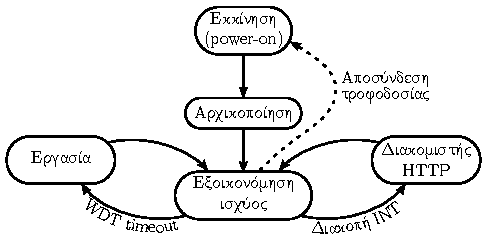
\includegraphics{mcu_tasks}
    \end{center}
\end{figure}

Αναλυτικότερα, κατά το στάδιο της αρχικοποίησης, τίθεται η συχνότητα του
ρολογιού του μικροελεκτή, η οποία, για τις ανάγκες της υλοποίησης, μειώνεται από
τα 16MHz στα 4MHz, και η κατεύθυνση των ακροδεκτών (δηλαδή ποιοι είναι εισόδου
και ποιοι εξόδου). Επίσης, ρυθμίζεται το κύκλωμα WDT (\te{Watch-Dog Timer}), το
οποίο είναι υπεύθυνο για την περιοδική αφύπνιση του μικροελεγκτή ώστε να
ελέγχεται η ανάγκη εκκίνησης νέου κύκλου μετρήσεων.

Επιπλέον, ανακτώνται οι μεταβλητές ρυθμίσεις της συσκευής είτε από τις
προκαθορισμένες (εργοστασιακές ρυθμίσεις), είτε από τις αποθηκευμένες τιμές της
εφεδρικής μνήμης, εφόσον αυτές είναι έγκυρες (βλ \nameref{subsec:backup-memory}
σ.~\pageref{subsec:backup-memory}).
Οι ρυθμίσεις αυτές περιλαμβάνουν τη δικτύωση της συσκευής (διεύθυνση IP, μάσκα
υποδικτύου, προεπιλεγμένη πύλη), το λειτουργικό εύρος του υποσυστήματος κίνησης
(βλ. \nameref{sec:motor:coordinates} σ.~\pageref{sec:motor:coordinates}), το
χρονικό διάστημα μεταξύ κύκλων εργασίας καθώς και το πλήθος μετρήσεων που
πραγματοποιείται σε κάθε κύκλο (βλ. \nameref{sec:task} σ.~\pageref{sec:task}).
Ο τρόπος ρύθμισης της συσκευής περιγράφεται στους Πόρους υλοποίησης (σ.~%
\pageref{sec:network:impl-resources}).

Στην πορεία, οι ρυθμίσεις προωθούνται στις κατάλληλες μονάδες και εκτελούνται
επιπρόσθετες προετοιμασίες, όπως η παλιννόστηση της κεφαλής, δηλαδή η επαναφορά
της στη θέση επιστροφής (συντεταγμένες [0, 0, Z\tsub{max}]) (βλ. σ.~%
\pageref{sec:motor:homing}) και η αρχικοποίηση του HTTP \te{Socket} (βλ. σ.~%
\pageref{ssubsec:network:port_mr}).


\subsection{Κατάσταση χαμηλής κατανάλωσης}

Ο μικροελεγκτής διαθέτει διάφορες καταστάσεις νάρκης (\te{sleep mode}
όπου η καθεμία απενεργοποιεί ορισμένα κυκλώματα για τη μείωση της κατανάλωσης.
Για παράδειγμα, η πιο απλή, είναι η κατάσταση αδράνειας (\te{idle}) κατά την
οποία απενεργοποιείται μόνο το ρολόι της CPU και της μνήμης Flash (δηλαδή, της
μνήμης προγράμματος). Στο πλαίσιο της υλοποίησης, γίνεται προσπάθεια για την
ύψιστη μείωση της κατανάλωσης κατά τα διαστήματα όπου ο μικροελεγκτής παραμένει
άεργος.

Για το σκοπό αυτό, εφαρμόζεται η κατάσταση \te{power-down} κατά την οποία
απενεργοποιούνται όλα τα ρολόγια του μικροελεγκτή (clk\tsub{CPU}, clk%
\tsub{FLASH}, clk\tsub{IO}, clk\tsub{ADC}, clk\tsub{ASY}) καθώς και οι
ταλαντωτές του συστήματος και των Χρονομετρητών\slash{}Απαριθμητών \parencite%
[38]{atmel13}. Σύμφωνα με την \textcite[38]{atmel13}, ο μικροελεγκτής είναι
δυνατό να επανέλθει σε κανονική λειτουργία μόνο μέσω των ακροδεκτών INT1:0 με
παρατεταμένο λογικό 0 (\te{low-level interrupt}) καθώς και μέσω των κυκλωμάτων
TWI (\te{Two-Wire Interface}) και WDT (\te{Watch-Dog Timer}).

Στο πλαίσιο της υλοποίησης χρησιμοποιείται ο πρώτος και ο τελευταίος τρόπος· το
κύκλωμα TWI αφυπνίζει το μικροελεγκτή όταν αυτός ρυθμίζεται με ρόλο \te{slave}
στο δίαυλο TWI και κάποιο εξωτερικό κύκλωμα προσπαθεί να επικοινωνήσει μαζί του
ενώ, στην υλοποίηση, χρησιμοποιείται μόνο ως \te{master} για την επικοινωνία με
το ρολόι πραγματικού χρόνου (RTC) (βλ. \nameref{sec:rtc} σ.~\pageref{sec:rtc}).

Για την ακρίβεια, ο ένας εκ των δύο ακροδεκτών INT1:0 συνδέεται με τον ακροδέκτη
\nbar{INT} του ολοκληρωμένου δικτύωσης, W5100, το οποίο τον θέτει και τον
διατηρεί σε λογικό 0 έως ότου διευθετηθούν όλες οι ενδείξεις διακοπών που του
έχουν ενεργοποιηθεί
(βλ. \nameref{subsec:network:interface} σ.~\pageref{subsec:network:interface}).
Για τις ανάγκες της υλοποίησης, αυτό σημαίνει ότι έχει καταφθάσει εισερχόμενο
αίτημα HTTP το οποίο διεκπεραιώνεται από το διακομιστή (βλ.
\nameref{sec:http-server} σ.~\pageref{sec:http-server}).

Ο χρονομετρητής WDT ρυθμίζεται ώστε να αφυπνίζει το μικροελεγκτή κάθε 8s (το
μέγιστο διάστημα που υποστηρίζεται από τον παρόντα μικροελεγκτή) και αποτελεί το
έναυσμα για την εκκίνηση νέου κύκλου εργασιών
(\nameref{ssubsec:task:initiate} σ.~\pageref{ssubsec:task:initiate}).


\section{Η υλοποίηση συνοπτικά}


\subsection{Κατασκευή}

Η κατασκευή της συσκευής γίνεται με χρήση ανοικτού (\te{open hardware})
συστήματος κατασκευής (\te{construction framework}), το \te{Open\-Builds}, για
την παροχή διαφόρων διευκολύνσεων (ράγες κίνησης, γραμμική κίνηση).

Η συσκευή είναι εμπνευσμένη από τη διάταξη κινητού γεφυρώματος (\te{moving
gantry}) εργαλειομηχανών CNC για την επίλυση των αναγκών της για γραμμική κίνηση
στο χώρο, με εξαίρεση ότι αφαιρείται η τράπεζα.
%Οι διαστάσεις της συσκευής είναι
Η κίνηση αφορά την κεφαλή, ένα εξάρτημα που φέρει αισθητήρες, και μετακινείται
σε επίπεδο πάνω από την επιφάνεια του παρακολουθούμενο υλικού και κατακόρυφα
προς αυτό για την πραγματοποίηση μετρήσεων. Η ύπαρξη της κινητής κεφαλής
επιτρέπει την αξιοποίηση ενός μικρού αριθμού αισθητήρων για την κάλυψη όλου του
παρακολουθούμενου υλικού. (Bλ. \nameref{ch:construction} σ.~%
\pageref{ch:construction}.)


\subsection{Κωδικοποίηση κίνησης}

Η μετατόπιση της κεφαλής πραγματοποιείται από κινητήρες. Η κίνησή τους
παρακολουθείται από κωδικοποιητή περιστροφικής κίνησης, ο οποίος παρέχει
ανατροφοδότηση στο μικροελεγκτή για τα, αναφερόμενα ως, βήματα που πραγματοποιεί
ο παρακολουθούμενος κινητήρας ώστε να αναγνωρίζει το μέγεθος της μετατόπισης.
Τέσσερα τέτοια βήματα (ή παλμοί) αποτελούν μία πλήρη περιστροφή.

Ο κωδικοποιητής είναι αυτοσχέδιος και χρησιμοποιεί ανακλαστικό αισθητήρα
υπερύθρων ακτίνων· μέρος της έντασης των ακτίνων που εκπέμπει ο πομπός που
διαθέτει, καταφθάνουν στο δέκτη του, αφού πρώτα ανακλαστούν σε λωρίδες
εναλλασσόμενης ανακλαστικότητας που κοσμούν την άτρακτο του κινητήρα. Παρέχεται
ένας κωδικοποιητής ανά κινητήρα.

Η απόσταση του αισθητήρα από την άτρακτο καθώς και το πλάτος των λωρίδων
επιλέγονται σύμφωνα με τις προδιαγραφές του αισθητήρα ώστε να ευνοείται η
ικανότητά του να διακρίνει τις εναλλαγές.

Ο κωδικοποιητής λειτουργείται με χαμηλή ένταση ρεύματος και μόνο κατά τα
διαστήματα που κινείται ο αντίστοιχος κινητήρας για τη μείωση της συνολικής
κατανάλωσης ισχύος της συσκευής και για την επιμήκυνση της διάρκειας ζωής του
(πομπού του) αισθητήρα. (Bλ. \nameref{ch:encoder} σ.~\pageref{ch:encoder}.)


\subsection{Υποσύστημα κίνησης}

Η θέση της κεφαλής προσδιορίζεται από σύστημα συντεταγμένων τριών αξόνων X, Υ
και Z. Η ελάχιστη μετατόπιση ανά άξονα ορίζεται ως μία πλήρη περιστροφή της
ατράκτου του κινητήρα, πρακτικά 4cm.

Το σήμα ελέγχου της κίνησης των κινητήρων παράγεται μέσω κυκλώματος
Χρονομετρητή\slash{}Απαριθμητή (\te{Timer\slash{}Counter}) του μικροελεγκτή.
Η λήξη της κίνησης αναλαμβάνεται από δεύτερο κύκλωμα Χρονομετρητη\slash{}%
Απαριθμητή ο οποίος καταμετρά το πλήθος των βημάτων του κωδικοποιητή και
τερματίζει την αναμετάδοση του σήματος κίνησης στον κινητήρα όταν ολοκληρώνεται
το προκαθορισμένο πλήθος βημάτων. Η χρήση του δεύτερου κυκλώματος
Χρονομετρητή\slash{}Απαριθμητή επιτρέπει την παύση της μετατόπισης ακόμα και εάν
η CPU του μικροελεγκτή είναι απασχολημένη.

Υλοποιείται παράλληλη κίνηση της κεφαλής στους άξονες X και Y η οποία βασίζεται
στην παραδοχή ότι επιτυγχάνεται, και για τους δύο άξονες, η ίδια γωνιακή
ταχύτητα για το χρονικό διάστημα κατά τον οποίο λειτουργούν παράλληλα. Πρακτικά,
αυτό αποτελεί μία από τις προκλήσεις της υλοποίησης και χρήζει βελτίωσης, όπως
αναφέρεται και παρακάτω (\nameref{sec:improvements} σ.~%
\pageref{sec:improvements}).

Για την κάλυψη κάθε ενδεχομένου, χρησιμοποιούνται ανασταλτικοί διακόπτες στις
άκρες της συσκευής (όρια αξόνων). Όταν κάποιος εξ αυτών ενεργοποιηθεί, η κεφαλή
επαναφέρεται σε μία συγκεκριμένη θέση (την αρχική ή θέση επιστροφής). Από εκεί,
επιχειρείται μία ακόμη φορά η εκ νέου μετάβαση στην θέση που προηγουμένως
κατέστη αδύνατ. Εφόσον ενεργοποιηθεί κάποιος διακόπτης ξανά, η μετάβαση
ακυρώνεται. (Bλ. \nameref{ch:motor} σ.~\pageref{ch:motor}.)


\subsection{Μετρήσεις}

Η ύπαρξης της κεφαλής συνδέεται με την πραγματοποίηση μετρήσεων οι οποίες
αποθηκεύονται στην εσωτερική μνήμη EEPROM του μικροελεγκτή. Οι, κατά μέγιστο, 90
πλέον πρόσφατες καταγεγραμμένες μετρήσεις, φέρουν την ημερομηνία και τη θέση στο
επίπεδο X-Y όπου πραγματοποιήθηκε, καθώς και τη θερμοκρασία που σημειώθηκε.
Η ημερομηνία\slash{}ώρα τηρείται από εξωτερικό ολοκληρωμένο ρολόι πραγματικού
χρόνου (RTC) το οποίο τροποποιείται, καταλλήλως, από το χρήστη.

Η διαχείριση των εγγραφών γίνεται από τη μονάδα του ημερολογίου (\te{log}), η
οποία είναι υπεύθυνη και για τη διατήρηση της εγκυρότητας των περιεχόμενων
εγγραφών. Σε περίπτωση που πραγματοποιηθεί μέτρηση σε ημερομηνία προγενέστερη
(σύμφωνα με την ώρα του RTC) σε σχέση με υπάρχουσες εγγραφές, το ημερολόγιο
εγγράφει τη νέα μέτρηση αποβάλλοντας τις προϋπάρχουσες προγενέστερες (λογική
διαγραφή και όχι φυσική για την μείωση φθορών στην EEPROM).

Μετρήσεις πραγματοποιούνται αυτόματα από τη συσκευή ανά σταθερά χρονικά
διαστήματα καθοριζόμενων από το χρήστη, σε ένα πλήθος τυχαία επιλεγμένων θέσεων.
Το πλήθος των μετρήσεων καθορίζεται, επίσης, από το χρήστη. Μία σειρά μετρήσεων
αναφέρεται ως εργασία και ξεκινά σε διαστήματα πολλαπλάσια των έξι λεπτών της
ώρας. Ο μέγιστος χρόνος αδράνειας της συσκευής που υποστηρίζεται είναι, πέραν
της εξ ολοκλήρου απενεργοποίησης των εργασιών, μία ημέρα. (Bλ.
\nameref{ch:foundation} σ.~\pageref{ch:foundation}.)


\subsection{Επικοινωνία με συσκευή}

Η επικοινωνία της συσκευής με εξωτερικές οντότητες γίνεται μέσω πρωτοκόλλου
HTTP· ο χρήστης αλληλεπιδρά μαζί της μέσω λογισμικού πλοήγησης (\te{browser})
ενώ τρίτα συστήματα, μέσω προγραμματιστικής διεπαφής (API).
Για την ακρίβεια, η ίδια η διεπαφή χρήστη αποτελεί έναν καταναλωτή αυτής της
προγραμματιστικής διεπαφής (API), και είναι υλοποιημένη με HTML5, CSS3 και
Javascript (χωρίς επιπρόσθετες βιβλιοθήκες) σε βαθμό ώστε να παρέχεται
συμβατότητα με τις περισσότερες εκδόσεις των δημοφιλέστερων λογισμικών πλοήγησης
και για εκδόσεις \te{Internet Explorer} 8 και άνω.

Τα δεδομένα που είναι απαραίτητα για τη διεπαφή του χρήστη (ιστοσελίδα και
αρχεία \@.css \@.js και εικόνων) εναποτίθενται σε εξωτερικό κύκλωμα μνήμης Flash
128KiB το οποίο χρησιμοποιείται μόνο για την ανάγνωσή τους και την επιστροφή
τους μέσω του υποσυστήματος διακομιστή HTTP.
Τα δεδομένα που ανταλλάσσονται μεταξύ τρίτων συστημάτων και συσκευής βρίσκονται
σε αναπαράσταση JSON (πέραν των HTML, CSS, Javascript και PNG που προορίζονται
για τη διεπαφή χρήστη).

Μέσω της διεπαφής της συσκευής δύναται η εμφάνιση των μετρήσεων που έχουν
πραγματοποιηθεί καθώς και οι ρυθμίσεις της συμπεριφοράς της. Οι ρυθμίσεις
διατηρούνται ακόμη και με την αποσύνδεση της συσκευής από την κεντρική
τροφοδοσία. Η επαναφορά τους στις εργοστασιακές (προκαθορισμένες) τιμές γίνεται
μέσω της προσωρινής απομάκρυνσης της μπαταρίας (\te{coin cell}) της συσκευής ενώ
αυτή είναι αποσυνδεδεμένη από την κεντρική τροφοδοσία.
Σημειώνεται ότι οι εργοστασιακές ρυθμίσεις απενεργοποιούν τις εργασίες, ενώ οι
ρυθμίσεις δικτύου είναι αυτές που ορίζονται στον πίνακα \ref{tab:default-ip}.
(Bλ. \nameref{ch:network} σ.~\pageref{ch:network}.)

\begin{table}
    \caption{Εργοστασιακές ρυθμίσεις δικτύωσης της συσκευής.
    \label{tab:default-ip}}
    \begin{center}
    \begin{tabu} to 6cm {X[L] *3{X[-2.5,R] @{.}} X[-1,R]}

    {\bfseries Διεύθυνση IP} :
        & 192 & 168 &   1 & 73 \\
    {\bfseries Προεπιλεγμένη πύλη} :
        & 192 & 168 &   1 &  1 \\
    {\bfseries Μάσκα υποδικτύου} :
        & 255 & 255 & 255 &  0 \\
    \end{tabu}\end{center}
\end{table}

%Αντιστοίχιση όρων
%PWM	        διαμόρφωση διάρκειας παλμών               Βιβλίο τηλεπικοινωνιών
%optocoupler	οπτικός συζεύκτης	           Reg. 1572/93 (1) OJ L 156/93 p.71
%sleep mode     κατάσταση νάρκης             Dec. 2001/469/EC OJ L 172/2001 p.11

\chapter{Βασικές λειτουργίες}
\label{ch:foundation}

Το κεφάλαιο αναφέρεται σε ορισμένες βασικές μονάδες της υλοποίησης

%Όπως συζητείται στο κεφάλαιο \nref{}
Ο μικροελεγκτής διαθέτει εσωτερική μνήμη EEPROM η οποία μπορεί να χρησιμοποιηθεί
για την αποθήκευση δεδομένων που διατηρούνται μεταξύ διαδοχικών απενεργοποιήσεων
του και η οποία, στην περίπτωση του ATmega328P, είναι χωρητικότητας 1KiB.
Η υλοποίηση έχει την ανάγκη για τη .. των αρχείων διεπαφής.
Οι απαιτήσεις των αρχείων αυτών σε αποθηκευτικό χώρο είναι δύσκολο να
ικανοποιηθούν είτε από τη μνήμη EEPROM είτε τη Flash του μικροελεγκτή, καθώς η
πρώτη ανέρχεται μόλις στο 1KiB, ενώ η δεύτερη, στα 32KiB, η οποία
χρησιμοποιείται, κατά κύριο λόγο, για την αποθήκευση του λογισμικού
(προγράμματος) του μικροελεγκτή και θα ήταν δύσκολο να χρησιμοποιηθεί και για
τα αρχεία της διεπαφής.
Για το λόγο αυτό επιλέγεται ένα ολοκληρωμένο μνήμης Flash χωρητικότητας 1024bit
(128KiB) για την αποθήκευση των αρχείων της διεπαφής (ιστοσελίδα, αρχείο
css \etc{.}). Τα δεδομένα της συγκεκριμένης μνήμης αρχικοποιούνται (δηλαδή,
εγγράφονται) σε ένα στάδιο πριν τον τελικό προγραμματισμό της συσκευής και, κατά
τη διάρκεια της κανονικής της λειτουργίας, η μνήμη χρησιμοποιείται μόνο για
ανάγνωση (βλ. \nameref{subsec:external-memory} σ.~%
\pageref{subsec:external-memory}).

Επιπλέον, ορίζεται μία εφεδρική μνήμη η οποία χρησιμεύει για την αποθήκευση των
ρυθμίσεων της συσκευής, δηλαδή τιμών που τίθενται από το χρήστη και επηρεάζουν
τη συμπεριφορά της συσκευής (βλ. σ.~\pageref{subsec:backup-memory}). Ο λόγος
ύπαρξής της είναι η διατήρηση των ρυθμίσεων μεταξύ διαδοχικών επανεκκινήσεων της
συσκευής. Χαρακτηρίζεται ως «εφεδρική» επειδή τα δεδομένα που εναποτίθενται σε
αυτήν θεωρούνται έγκυρα όσο η εφεδρική τροφοδοσία της συσκευής είναι διαθέσιμη,
ενώ επαναφέρονται στις προκαθορισμένες τιμές (τις εργοστασιακές ρυθμίσεις)
εφόσον και αυτή (επιπροσθέτως της κύριας τροφοδοσίας) απενεργοποιηθεί προσωρινά.
Η εφεδρική τροφοδοσία πρόκειται για μία συστοιχία συσσωρευτών (μπαταρία) που
επιτρέπει στο ρολόι πραγματικού χρόνου (RTC) να λειτουργεί κατά τα διαστήματα
που η συσκευή είναι αποσυνδεδεμένη από την κύρια τροφοδοσία (δηλαδή, όταν η
συσκευή είναι απενεργοποιημένη).
\begin{figure}
    \caption{Σχέσεις μεταξύ των βασικών μονάδων της υλοποίησης.
    \label{fig:foundation:lvl-0}}
    \begin{center}
    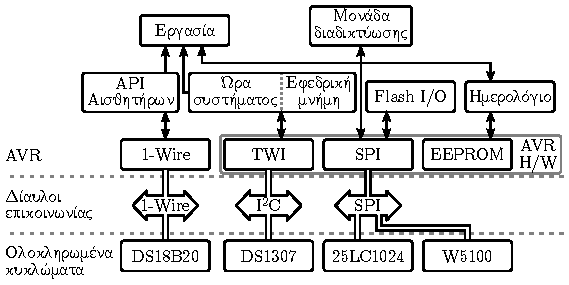
\includegraphics{foundation_lvl-0}
    \end{center}
\end{figure}

Στη συνέχεια αναλύεται το λογισμικό που είναι υπεύθυνο για τη διαχείριση των
μετρήσεων, το Ημερολόγιο (\pageref{sec:log}). Το Ημερολόγιο αναλαμβάνει την
αποθήκευση και ανάκτηση εγγραφών οι οποίες περιέχουν, υποχρεωτικά, ημερομηνία%
\slash{}ώρα και ένα πλήθος επιπρόσθετων Byte. Οι εγγραφές επιστρέφονται σε
φθίνουσα σειρά βάσει της ημερομηνίας\slash{}ώρας κάθε εγγραφής ενώ η ανάκτησή
τους υλοποιείται με τρόπο που διευκολύνει τη σελιδοποίηση των εγγραφών στο
πλαίσιο αναζητήσεων (βλ. \nameref{subsec:network:measurement} σ.~%
\pageref{subsec:network:measurement}).

Ο αποθηκευτικός χώρος των εγγραφών του Ημερολογίου έχει επιλεγεί να είναι η
εσωτερική μνήμη EEPROM του μικροελεγκτή (1 KiB). Πρακτικά, αυτό σημαίνει ότι το
Ημερολόγιο είναι ρυθμισμένο να διατηρεί τις 90 πλέον πρόσφατες μετρήσεις,
αφήνοντας μερικά Byte (34) για ενδεχόμενα άλλα δεδομένα.

Κατόπιν, ακολουθεί περιγραφή της διευθέτησης και χειρισμού του ρολογιού
πραγματικού χρόνου (\te{RTC -- Real-Time Clock}), ένα ολοκληρωμένο που παρέχει
στη συσκευή τη δυνατότητα αναγνώρισης της τρέχουσας ημερομηνίας\slash{}ώρας
(βλ. \nameref{sec:rtc} σ.~\pageref{sec:rtc}). Στο παρόν στάδιο της υλοποίησης,
το ολοκληρωμένο χρησιμοποιείται για την αναγνώριση του χρόνου που έχει παρέλθει
από την τελευταία μέτρηση του Ημερολογίου ώστε να αποφασίζεται εάν πρέπει να
εκκινηθεί νέος κύκλος μετρήσεων. Ο σχετικός έλεγχος πραγματοποιείται κάθε 8s από
ξεχωριστή μονάδα, όταν ο μικροελεγκτής αφυπνίζεται από εσωτερικό κύκλωμά
του, το \te{Watch-Dog Timer} (WDT).

Η υπεύθυνη μονάδα για την εκτέλεση των μετρήσεων -- όπου στο πλαίσιο της
υλοποίησης περιλαμβάνουν μόνο τη θερμοκρασία -- είτε με αυτόματο τρόπο είτε μη
περιγράφεται στην \nameref{sec:task} (σ.~\pageref{sec:task}). Στο πλαίσιο της,
παρέχεται, επιπροσθέτως, η δυνατότητα εκτίμησης του χρόνου ολοκλήρωσης της
τρέχουσας εργασίας (είτε αυτή αναφέρεται σε μεμονωμένη ή αλληλουχία μετρήσεων,
είτε σε απλή μετακίνηση της κεφαλής) το οποίο αξιοποιείται κατά την απόκριση σε
ορισμένα αιτήματα (βλ. \nameref{sec:network:impl-resources} σ.~%
\pageref{sec:network:impl-resources}).

Τέλος, αναλύονται οι δίαυλοι και το λογισμικό οδήγησης που χρησιμοποιούνται για
την επικοινωνία μεταξύ του μικροελεγκτή και των διαφόρων εξωτερικών
ολοκληρωμένων. Συνολικά, γίνεται χρήση των διαύλων 1-Wire, Ι\tsup{2}C και SPI
(βλ. \nameref{sec:buses} σ.~\pageref{sec:buses}).

Οι σχέσεις μεταξύ των διαφόρων μονάδων που αναλύονται σε αυτό το κεφάλαιο,
εμφανίζονται στο σχήμα \ref{fig:foundation:lvl-0}, με εξαίρεση του Υποσυστήματος
κίνησης και της Διαδικτύωσης τα οποία διαθέτουν ξεχωριστά κεφάλαια (βλ.
σ.~\pageref{ch:motor} και σ.~\pageref{ch:network}, αντίστοιχα).

%    Μνήμη προγράμματος
%    Εξοικονόμηση ενέργειας

\section{Μνήμες αποθήκευσης}

\subsection{Αρχεία διεπαφής}
\label{subsec:external-memory}

Κρίνεται σκόπιμη η ύπαρξη ενός αφιερωμένου αποθηκευτικού μέσου για την εναπόθεση
των αρχείων της διεπαφής της συσκευής (ιστοσελίδα, κώδικας javascript \etc{.} --
βλ. \nameref{subsec:network:files} σ.~\pageref{subsec:network:files}) καθώς οι,
εσωτερικά, διαθέσιμες μνήμες του μικροελεγκτή -- 32KiB μνήμη προγράμματος και
1KiB μνήμη EEPROM -- θεωρείται ότι αδυνατούν να τα υποστηρίξουν ή θα έθεταν
αισθητούς περιορισμούς στο μέγεθός τους και, συνεπώς, στη λειτουργικότητα της
διεπαφής.

Για το σκοπό αυτό, επιλέγεται το ολοκληρωμένο 25LC1024 το οποίο διαθέτει 128KiB
μνήμη EEPROM, χωρισμένη σε τέσσερις τομείς των 32KiB με 128 σελίδες ο καθένας,
με δυνατότητα εγγραφής σε επίπεδο Byte ή σελίδας και διασύνδεση μέσω διαύλου SPI
\parencite[1]{25lc1024}. Για λεπτομέρειες σχετικά με το δίαυλο SPI, βλ. σ.~%
\pageref{subsec:spi}. Κρίνεται ότι η χωρητικότητά του είναι υπεραρκετή για τις
τρέχουσες, ή άμεσα μελλοντικές, ανάγκες της υλοποίησης.
Στο παρόν στάδιο της υλοποίησης, η αποθήκευση των αρχείων στη μνήμη γίνεται σε
αυθαίρετα επιλεγμένες διευθύνσεις μνήμης, οι οποίες δηλώνονται κατά τη σύνταξη
του προγράμματος, ενώ τα αρχεία είναι αδύνατο να μεταβληθούν μέσα από την
υλοποίηση.

Η πρόσβαση της μνήμης του ολοκληρωμένου για την ανάγνωση και εγγραφή των κελιών
της γίνεται μέσω ορισμένων εντολών. Το σύνολο των εντολών μπορεί να χωριστεί σε
τρεις κατηγορίες· εντολές ανάγνωσης, εγγραφής και ειδικής χρήσης, καθεμία από
τις οποίες μελετάται ξεχωριστά. Στη γενική τους μορφή, όλες οι εντολές
περιγράφονται από τους ακόλουθους κανόνες:
\begin{lstlisting}
command     = instruction_code [ load ]
load        = memory_cell | octet
memory_cell = address *octet
\end{lstlisting}
Οι κωδικοί εντολών έχουν μήκος 8bit ενώ οι διευθύνσεις, 24bit εκ των οποίων τα
πρώτα 7 αγνοούνται από το ολοκληρωμένο καθώς τα υπολειπόμενα 17 είναι ικανά για
την αναφορά στις 128KiB διαθέσιμες θέσεις \parencite[6--7]{25lc1024}. Σαφώς,
τα πραγματικά μέρη που συνθέτουν την εκάστοτε εντολή εξαρτώνται από τον κωδικό
και, συνεπώς, τη λειτουργία της. Για παράδειγμα, η διεύθυνση κελιού μνήμης
(\te{\verb~address~}) έχει νόημα για τις εντολές ανάγνωσης, εγγραφής και
απαλοιφής μέρους της μνήμης, ενώ η απαλοιφή όλων των δεδομένων της μνήμης
(\te{Chip Erase}) απαιτεί μόνο τον κωδικό της (\te{\verb~instruction\_code~}).

Ωστόσο, όλες οι εντολές προϋποθέτουν ότι το 25LC1024 βρίσκεται σε κατάσταση
ετοιμότητας (δηλαδή, όχι σε κατάσταση χαμηλής κατανάλωσης ισχύος), ενώ ενδέχεται
να ισχύουν επιπρόσθετοι περιορισμοί, ανάλογα με την εντολή
\parencite[17]{25lc1024}.


\subsubsection{Ανάγνωση}
\label{ssubsec:25lc1024:read-commands}

Οι εντολές ανάγνωσης επιτρέπουν την ανάκτηση δεδομένων από τα κελιά της μνήμης
καθώς και την τιμή του καταχωρητή κατάστασης SR (\te{Status Register}) -- του
μοναδικού καταχωρητή του ολοκληρωμένου -- ο οποίος παρέχει στοιχεία για την
πορεία ενδεχόμενων εγγραφών και έλεγχο γύρω από την ενεργοποίηση της εγγραφής
(περισσότερα βλ. \nameref{ssubsec:25lc1024:write-protect}
σ.~\pageref{ssubsec:25lc1024:write-protect}).

Σύμφωνα με τη \textcite[6]{25lc1024}, το ολοκληρωμένο αγνοεί τις απόπειρες
ανάγνωσης μνήμης όταν βρίσκεται σε εξέλιξη εγγραφή δεδομένων, δηλαδή όσο η
ένδειξη WIP (\te{Write-In-Progress}) του καταχωρητή κατάστασης βρίσκεται σε
λογικό 1.

Ως εντολές ανάγνωσης μπορούν να χαρακτηριστούν οι ακόλουθες:
\begin{description}
    \item[READ [0x03{]}] Επιστρέφει το \te{Byte} της μνήμης που βρίσκεται στην
    προσδιοριζόμενη διεύθυνση και συνεχίζει με κάθε επόμενο για διαδοχικούς
    παλμούς της ίδιας εντολής, αυτομάτως μεταβαίνοντας στη διεύθυνση 0 ως το
    επόμενο \te{Byte} της τελευταίας διεύθυνσης \parencite[6--7]{25lc1024}.
    Προφανώς, η σύνταξη της εντολής απαιτεί διεύθυνση και τουλάχιστον ένα
    \te{Byte} δεδομένων.

    \item[RDSR [0x05{]}] (\te{ReaD Status Register}) Επιστρέφει την τιμή του
    καταχωρητή κατάστασης του ολοκληρωμένου και απαιτεί, επιπροσθέτως του
    κωδικού εντολής, ένα \te{Byte} \parencite[10]{25lc1024}.

    \item[RDID [0xAB{]}] (\te{ReaD ID}) Επιστρέφει το αναγνωριστικό της συσκευής
    και την αφυπνίζει από την κατάσταση χαμηλής κατανάλωσης ισχύος, εάν έχει
    τεθεί σε αυτήν. Η εντολή απαιτεί την αποστολή 24bit διεύθυνσης (τα οποία
    χρησιμοποιούνται για την προετοιμασία του ολοκληρωμένου, χωρίς να έχει
    ιδιαίτερη σημασία η τιμή τους), και ένα \te{Byte} για την επιστροφή του
    αναγνωριστικού (ή «υπογραφής») του \parencite[17]{25lc1024}
    \label{ssubsec:25lc1024:read-commands:rdid}.

    Για την εντολή μετάπτωσης σε κατάσταση χαμηλής κατανάλωσης ισχύος, βλ.
    \nameref{ssubsec:25lc1024:special-commands} (σ.~%
    \pageref{ssubsec:25lc1024:special-commands}).
\end{description}


\subsubsection{Εγγραφή και προστασία}
\label{ssubsec:25lc1024:write-protect}

Ως εγγραφή νοείται τόσο η αποστολή δεδομένων (Byte) από το μικροελεγκτή με
προορισμό τον καταχωρητή κατάστασης SR του ολοκληρωμένου ή συγκεκριμένες θέσεις
της μνήμης EEPROM, είτε η \emph{απαλοιφή} των δεδομένων από τα κελιά της μνήμης
και την επαναφορά τους στην προκαθορισμένη τιμή 0xFF (\te{erase})
\parencite[6--7]{25lc1024}.

Ωστόσο, για την αποφυγή μη εσκεμμένων (τυχαίων) εγγραφών στις θέσεις μνήμης με
αποτέλεσμα την αλλοίωση των δεδομένων, το ολοκληρωμένο απαιτεί τη δήλωση της
πρόθεσης για εγγραφή. Επιπλέον, παρέχονται δύο επιπρόσθετα επίπεδα προστασίας
ώστε να μειώνεται περαιτέρω η πιθανότητα ακούσιας τροποποίησης των δεδομένων από
αστοχίες υλικού και εξωτερικών παρεμβολών.

\paragraph{Μανδαλωτής WEL} Αρχικά, προκειμένου να εκτελεστεί οποιαδήποτε εντολή
εγγραφής, απαιτείται να προηγηθεί η αποστολή της εντολής WREN
(\te{WRite ENable}) ώστε να ενεργοποιηθεί ο μανδαλωτής WEL (\te{Write-Enable
Latch}) \parencite[6]{25lc1024}.
Κατόπιν, απενεργοποιείται η γραμμή \nbar{CS} (τίθεται σε λογικό 1) και
ενεργοποιείται ξανά (λογικό 0) για την αποστολή της εντολής εγγραφής. Ο
μανδαλωτής WEL απενεργοποιείται είτε αυτόματα με την ολοκλήρωση της εγγραφής
ή κατά την αρχική τροφοδοσία του ολοκληρωμένου με τάση (\te{power-on}) είτε
μέσω της, ειδικής για αυτόν τον σκοπό, εντολής WRDI (\te{WRite DIsable})
\parencite[9]{25lc1024}. Αυτό το επίπεδο προστασίας είναι το μοναδικό που
εφαρμόζεται υποχρεωτικά.

\begin{table}
    \caption{
    \label{tab:25lc1024:bp-bits}}
    \begin{center}\begin{tabu} spread 0pt {*2{X[-1,C]} X[2,L]}
    \rowfont\bfseries
    BP1 &   BP0 & Προστατευμένη περιοχή                                       \\
    \hline
      0 &     0 & Καμία                                                       \\
      0 &     1 & 3\tsup{ος} τομέας (0x18000--0x1FFFF)                        \\
      1 &     0 & 2\tsup{ος} και 3\tsup{ος} τομέας (0x10000--0x1FFFF)         \\
      1 &     1 & Όλοι οι τομείς (0x00000--0x1FFFF)                           \\
    \end{tabu}\end{center}

    Βασισμένο \fullcite[11]{25lc1024:bp-bits}
\end{table}

\paragraph{Προστατευμένες περιοχές} Ως ένα επιπρόσθετο επίπεδο ασφαλείας είναι
δυνατό να οριστεί, μέσω των \te{bit} BP1:0 του καταχωρητή SR, ποιος συνδυασμός
τομέων θα είναι «προστατευμένος από εγγραφή», με την έννοια ότι η εγγραφή στις
θέσεις μνήμης αυτών των τομέων απενεργοποιείται, εκτός και εάν προηγηθεί
τροποποίηση αυτής της ρύθμισης σε προγενέστερο χρόνο της εντολής εγγραφής
\parencite[10,12]{25lc1024}. Οι δυνατοί συνδυασμοί παρουσιάζονται στον πίνακα
\ref{tab:25lc1024:bp-bits}.

\paragraph{Προστασία καταχωρητή SR} Το τελευταίο στάδιο προστασίας αφορά τον
καταχωρητή SR και συμπεριλαμβάνει το χειρισμό του ακροδέκτη \nbar{WP} του
ολοκληρωμένου επιπροσθέτως του μανδαλωτή WEL προκειμένου να επιτραπεί η
τροποποίηση των μη πτητικών \te{bit} του καταχωρητή SR (δηλαδή των \te{bit} WPEN
και BP1:0) \parencite[10--12]{25lc1024}. Η ενεργοποίηση αυτού του επιπέδου
προστασίας πραγματοποιείται από το \te{bit} WPEN (\te{Write-Protect ENable}) του
καταχωρητή SR. Εφόσον η δυνατότητα εγγραφής του καταχωρητή επαναφερθεί,
ακολουθεί τροποποίηση των \te{bit} BP1:0 ώστε να επιτραπεί πρόσβαση στις
προστατευμένες περιοχές.

\begin{table}
    \caption{Επίπεδα προστασίας από εγγραφή.
    \label{tab:25lc1024:protection}}
    \begin{center}\begin{tabu} spread 0pt {*3{X[-1,C]} | *3{X[-1,C]}}
    \rowfont\bfseries
    WEL        &       WPEN & \nbar{WP} & Περιοχή & Υπόλοιπη & Καταχωρητής    \\
    \rowfont\bfseries
    (SR bit 1) & (SR bit 7) &   (pin 3) &   BP1:0 &   μνήμη  &        SR\\\hline
    0          &          X &         X &     ναι &      ναι &         ναι    \\
    1          &          0 &         X &     ναι &      όχι &         όχι    \\
    1          &          1 &   0 (low) &     ναι &      όχι &         ναι    \\
    1          &          1 &  1 (high) &     ναι &      όχι &         όχι
    \end{tabu}\end{center}
    \noindent
    \begin{tabu} spread 0pt {X[-1] @{ : } X}
    X   & αδιάφορο                      \\
    ναι & προστατευμένο από εγγραφή     \\
    όχι & εγγράψιμο
    \end{tabu}

    Βασισμένο \fullcite[12]{25lc1024:protection}
\end{table}

Τα τρία επίπεδα προστασίας από εγγραφή παρουσιάζονται στον πίνακα
\ref{tab:25lc1024:protection} ενώ οι εντολές που υπάγονται στην κατηγορία
εγγραφής αναφέρονται παρακάτω. Όλες οι εντολές αυτές υπόκεινται στην προστασία
εγγραφής και αγνοούνται εάν, τη στιγμή υποβολής τους, ο μανδαλωτής WEL είναι
απενεργοποιημένος ή εάν αναφέρονται σε κελί μνήμης που ανήκει σε προστατευμένη
περιοχή (βλ. πίνακα \ref{tab:25lc1024:bp-bits}). Για την ακρίβεια, ακόμα και οι
εντολές SE και CE που εφαρμόζονται σε πολλαπλούς τομείς, αγνοούνται ολοκληρωτικά
σε περίπτωση που αναφέρονται έστω και σε έναν προστατευμένο τομέα
\parencite[14--15]{25lc1024}.

\begin{description}
    \item[WREN [0x06{]}] (\te{WRite ENable}) Όχι ακριβώς εντολή εγγραφής αλλά
    άμεσα σχετιζόμενη. Όπως έχει αναφερθεί, προκειμένου να πραγματοποιηθεί
    εγγραφή στη μνήμη ή στον καταχωρητή κατάστασης, πρέπει πρώτα να
    ενεργοποιηθεί ο μανδαλωτής WEL (\te{Write-Enable Latch})
    \parencite[6]{25lc1024}.
    Η εντολή WREN κάνει ακριβώς αυτό για την επόμενη εντολή εγγραφής που
    αποστέλλεται στο ολοκληρωμένο, ενώ ταυτόχρονα θέτει την ένδειξη WEL
    (\te{Write-Enable Latch}) του καταχωρητή κατάστασης
    \parencite[10]{25lc1024}. Η εντολή WREN αποτελείται μόνο από τον κωδικό της.

    \item[WRDI [0x04{]}] (\te{WRite DIsable}) Απενεργοποιεί χειροκίνητα το
    μανδαλωτή WEL χωρίς την εκτέλεση κάποιας εντολής εγγραφής
    \parencite[9]{25lc1024}. Και αυτή η εντολή αποτελείται μόνο από τον κωδικό
    της.

    \item[WRITE [0x02{]}] Επιτρέπει την αποστολή ενός ή περισσοτέρων \te{Byte}
    για εγγραφή στη μνήμη, υποχρεωτικά εντός \emph{μίας} συγκεκριμένης σελίδας,
    ξεκινώντας από την προσδιοριζόμενη διεύθυνση εκείνης της σελίδας
    \parencite[6,8]{25lc1024}. Τα αποστελλόμενα \te{Byte} εναποτίθενται σε
    προσωρινό χώρο αποθήκευσης του ολοκληρωμένου (μέγιστης χωρητικότητας, το
    μέγεθος σελίδας -- 256Byte), ενώ η πραγματική εγγραφή ξεκινάει και
    πραγματοποιείται ασύγχρονα κατόπιν απενεργοποίησης της γραμμής
    \nbar{CS} \parencite[6]{25lc1024}.

    Η ολοκλήρωση της εγγραφής σηματοδοτείται μέσω της ένδειξης WIP
    (\te{Write-In-Progress}) του καταχωρητή κατάστασης, ενώ κατά τη διάρκεια της
    εγγραφής, η μνήμη είναι αδύνατο να προσπελαστεί για πάσης φύσεως λειτουργία
    \parencite[6]{25lc1024}.

    \item[WRSR [0x01{]}] (\te{WRite Status Register}) Επιτρέπει την αλλαγή των
    μη πτητικών \te{bit} του καταχωρητή (δηλαδή των \te{bit} WPEN και BP1:0) που
    ελέγχουν τις προστατευμένες περιοχές της μνήμης
    \parencite[10--11]{25lc1024}. Ο κωδικός εντολής ακολουθείται από ένα Byte
    που περιέχει τις νέες ρυθμίσεις.

    \item[PE [0x42{]}] (\t{Page Erase}) Δέχεται μία διεύθυνση και θέτει σε 0xFF
    όλα τα κελιάς της σελίδας στην οποία αυτή ανήκει \parencite[13]{25lc1024}.

    \item[SE [0xD8{]}] (\te{Sector Erase}) Αντίστοιχη της PE με τη διαφορά ότι
    εφαρμόζεται στις θέσεις μνήμης ολόκληρου του τομέα που περιέχει την
    αναφερόμενη διεύθυνση \parencite[14]{25lc1024}.

    \item[CE [0xC7{]}] (\te{Chip Erase}) Αντίστοιχη των PE και SE μόνο που
    εφαρμόζεται σε ολόκληρη τη μνήμη \parencite[15]{25lc1024}.
\end{description}

Για την υλοποίηση κρίνεται αρκετή η χρήση του πρώτου (και υποχρεωτικού) επιπέδου
προστασίας (μανδαλωτής WEL) κυρίως επειδή εγγραφή στη μνήμη πραγματοποιείται
μόνο κατά την αρχική ρύθμιση του συστήματος και όχι κατά την τυπική του
λειτουργία. Για την ακρίβεια, ο κώδικας που είναι υπεύθυνος για την εγγραφή των
αρχείων της διεπαφής στη μνήμη χρησιμοποιείται μόνο προσωρινά και εξαιρείται από
τον τελικό κώδικα που εγγράφεται στη μνήμη προγράμματος του μικροελεγκτή.


\subsubsection{Ειδικές εντολές}
\label{ssubsec:25lc1024:special-commands}

Σε αυτήν την κατηγορία συγκαταλέγονται οι εντολές που ελέγχουν πρόσθετες
λειτουργίες του ολοκληρωμένου, ουσιαστικά, την κατάσταση χαμηλής κατανάλωσης
ισχύος \parencite[16]{25lc1024}.

\begin{description}
    \item[RDID [0xAB{]}] (\te{ReaD ID}) Επιστρέφει το αναγνωριστικό της συσκευής
    και την αφυπνίζει από την κατάσταση χαμηλής κατανάλωσης ισχύος
    \parencite[17]{25lc1024}. Παρότι έχει συμπεριληφθεί στην κατηγορία εντολών
    ανάγνωσης επειδή πραγματοποιεί \emph{ανάγνωση} του αναγνωριστικού του
    ολοκληρωμένου (βλ. σ.~\pageref{ssubsec:25lc1024:read-commands:rdid}),
    αναφέρεται και σε αυτήν την κατηγορία για λόγους πληρότητας.

    \item[DPD [0xB9{]}] (\te{Deep Power-Down}) Θέτει το ολοκληρωμένο σε
    κατάσταση χαμηλής κατανάλωσης ισχύος κατά την οποία όλες οι εντολές
    αγνοούνται, με εξαίρεση της RDID που χρησιμοποιείται για την αφύπνισή του
    \parencite[16]{25lc1024}
\end{description}


\subsection{Εφεδρική μνήμη}
\label{subsec:backup-memory}

Η συσκευή διαθέτει ένα πλήθος ρυθμίσεων που είναι δυνατό να τροποποιηθούν από το
χρήστη ώστε να προσαρμόζεται η συμπεριφορά της σε διαφορετικές απαιτήσεις, όπως,
για παράδειγμα, το χρονικό διάστημα μεταξύ μετρήσεων, το λειτουργικό εύρος
(δηλαδή, οι διαστάσεις του παρακολουθούμενου χώρου) και οι δικτυακές ρυθμίσεις
της συσκευής. Περισσότερα σχετικά με τις υποστηριζόμενες ρυθμίσεις περιγράφονται
στην ενότητα \nameref{subsec:network:config} (σ.~%
\pageref{subsec:network:config}).

Όπως είναι αναμενόμενο, οι ρυθμίσεις πρέπει να διατηρούνται μεταξύ διαδοχικών
επανεκκινήσεων της συσκευής, είτε αυτές οφείλονται σε προγραμματισμένες
εργασίες συντήρησης είτε σε απρόσμενα περιστατικά (παραδείγματα, μετακίνηση σε
νέο χώρο ή διακοπή ρεύματος, αντίστοιχα). Αυτομάτως, η χρήση μόνο της κύριας
μνήμης του μικροελεγκτή για την τήρησή τους κρίνεται ακατάλληλη, καθώς πρόκειται
για πτητική μνήμη (για την ακρίβεια, \te{Static RAM}) με αποτέλεσμα, σε κάθε
επανεκκίνηση της συσκευής να ανακτώνται οι προκαθορισμένες τιμές του
προγράμματος και όχι οι δηλωμένες από το χρήστη.

Επομένως, απαιτείται μία επιπρόσθετη, πιο μόνιμη μορφή αποθήκευσης των
ρυθμίσεων, με άμεσους υποψηφίους, την εσωτερική μνήμη EEPROM 1KiB του
μικροελεγκτή ή την εξωτερική μνήμη \te{Flash} (ολοκληρωμένο 25LC1024, βλ. σ.~%
\pageref{subsec:external-memory}). Ανεξαρτήτως της επιλογής, θα πρέπει να
δίνεται στο χρήστη η δυνατότητα επαναφοράς στις προκαθορισμένες (ή
εργοστασιακές) ρυθμίσεις της συσκευής για την αντιμετώπιση περιπτώσεων αδυναμίας
τροποποίησής τους μέσω της διεπαφής. Αντιπροσωπευτικό τέτοιο παράδειγμα αποτελεί
η απώλεια της διεύθυνσης IP που έχει αποδοθεί στη συσκευή. Δεδομένου ότι στο
τρέχον στάδιο της υλοποίησης υποστηρίζεται μόνο χειροκίνητη απόδοση διεύθυνσης,
η διεπαφή είναι αδύνατο να προσπελαστεί εφόσον είναι άγνωστη η διεύθυνση IP της.

Η λύση παρέχεται από το RTC (\te{Real-Time Clock}) που χρησιμοποιείται για την
τήρηση της τρέχουσας ημερομηνίας και ώρας. Όπως περιγράφεται στη σχετική ενότητα
\nameref{sec:rtc} (σ.~\pageref{sec:rtc}), το RTC τροφοδοτείται από την κεντρική
γραμμή τροφοδοσίας της συσκευής και, σε περίπτωση πτώσης της σε χαμηλότερα
επίπεδα από την εφεδρική τάση του RTC, μεταπίπτει αυτομάτως στη χρήση της
δεύτερης. Εάν για κάποιο λόγο και η εφεδρική τροφοδοσία διακοπεί, το RTC παύει
να λειτουργεί και παραμένει απενεργοποιημένο ακόμη και κατόπιν επαναφοράς της
τροφοδοσίας.

Το ολοκληρωμένο διαθέτει σχετική ένδειξη λειτουργίας το οποίο μπορεί να ελεγχθεί
προκειμένου να αποφασιστεί η ανάκτηση είτε των αποθηκευμένων ρυθμίσεων του
χρήστη είτε οι εργοστασιακές. Εφόσον στο πλαίσιο της υλοποίησης η εφεδρική
τροφοδοσία παρέχεται μέσω συστοιχίας συσσωρευτών, η επαναφορά στις εργοστασιακές
ρυθμίσεις
μπορεί, πολύ εύκολα, να πραγματοποιηθεί με την προσωρινή απομάκρυνση της
μπαταρίας ενώ η συσκευή είναι απενεργοποιημένη.

Ωστόσο, σημειώνεται ότι, στην περίπτωση της υλοποίησης, για την αποθήκευση των
ρυθμίσεων χρησιμοποιείται η, γενικού σκοπού, μνήμη του RTC αντί κάποιας εκ των
προαναφερθεισών μνημών EEPROM.
Ο μόνος άμεσος περιορισμός είναι η χωρητικότητα της μνήμης του RTC -- 56Byte --
που για την υλοποίηση, ο χώρος αυτός είναι αρκετός.

Ωστόσο, στην περίπτωση της υλοποίησης, και δεδομένου ότι διατίθεται σχετική
υποδομή, χρησιμοποιείται η, γενικού σκοπού, μνήμη του RTC (\te{Real-Time Clock})
των 56Byte (βλ. \nameref{subsec:rtc:user-ram} σ.~\pageref{subsec:rtc:user-ram}).
Ένας βασικός περιορισμός είναι το συνολικά διαθέσιμο μέγεθος. Τα 56Byte που
διαθέτει το RTC είναι αρκετά για τις ανάγκες της υλοποίησης. Σε διαφορετική

%\subsection{Μετρήσεις αισθητήρων}
% internal EEPROM : mention that not all space is assigned for the Log


\section{Ημερολόγιο}
\label{sec:log}

Μία αναμενόμενη απαίτηση της υλοποίησης είναι η διατήρηση των μετρήσεων για την
μετέπειτα ανάκτηση και επεξεργασία τους με σκοπό την εξαγωγή συμπερασμάτων ή τη
λήψη αποφάσεων για την κατάσταση του μέσου. Το Ημερολόγιο μετρήσεων αναλαμβάνει
τη διαχείριση εγγραφών που παρέχουν αυτήν την πληροφορία. Ωστόσο το περιεχόμενο
και η εγκυρότητα κάθε εγγραφής επαφίεται σε τρίτα υποσυστήματα που υποβάλλουν
τις εκάστοτε μετρήσεις.

Η τήρηση του ημερολογίου έχει επιλεγεί να γίνεται στην εσωτερική μνήμη EEPROM
του μικροελεγκτή, χωρητικότητας 1KiB.

%Περιορισμοί EEPROM (χωρητικότητα και πλήθος επανεγγραφών)

%
% LogRecord
%

\subsection{Δομή εγγραφής}

Σημείο κεντρικού ενδιαφέροντος του Ημερολογίου είναι οι εγγραφές.
Καθότι ανήκει σε ημερολόγιο, κάθε εγγραφή είναι άρρηκτα συνδεδεμένη με μία
ημερομηνία\slash ώρα (εφεξής αναφερόμενη απλά ως «ημερομηνία»), που προσδιορίζει
τη χρονική τοποθέτησή της και χρησιμεύει ως κριτήριο αναζήτησης -- το μοναδικό
που υποστηρίζεται από το Ημερολόγιο σε αυτήν την υλοποίηση.
Εκτός από την ημερομηνία, τηρούνται και τα στοιχεία της μέτρησης, όπως οι
συντεταγμένες όπου έγινε η δειγματοληψία και, σαφώς, οι ενδείξεις των
αισθητήριων οργάνων. Το σχήμα \ref{fig:log:record} παρουσιάζει τη δομή κάθε
εγγραφής.

\begin{figure}
    \caption{Δομή μίας εγγραφής Ημερολογίου.\label{fig:log:record}}
\begin{center}\begin{tabu} spread 0pt {|X|X|X|X|X|X|X|X|X|X|X|}

    \multicolumn6{c}{
        $\overbrace{\rule{4cm}{0pt}}^{\text{ημερομηνία}}$}              &
    \multicolumn5{c}{
        $\overbrace{\rule{3.2cm}{0pt}}^{\text{στοιχεία μέτρησης}}$}     \\

    \hline\rowfont[c]{}
    \verb~YY~           &
    \verb~ΜΜ~           &
    \verb~DD~           &
    \verb~HH~           &
    \verb~mm~           &
    \verb~ss~           &
    \verb~X~            &
    \verb~Y~            &
    \verb~Τ~            &
    \verb~RH~           &
    \verb~pH~           \\
    \hline

\end{tabu}\end{center}\end{figure}

Είναι φανερό ότι η ημερομηνία καταλαμβάνει ένα πολύ μεγάλο μέρος της εγγραφής
και ο λόγος είναι ότι αναπαριστάται σε BCD. Ο συμβολισμός BCD
(\textenglish{Binary-Coded Decimal notation} -- Δυαδικά Κωδικοποιημένος
Δεκαδικός συμβολισμός), όπως
χρησιμοποιείται στην προκειμένη, απαιτεί ένα Byte για την αναπαράσταση
οποιουδήποτε αριθμού του δεκαδικού συστήματος αρίθμησης από 0 μέχρι 99· εύρος
ικανό να καλύψει τις ανάγκες του Ημερολογίου.

Κύριος λόγος για την επιλογή του συμβολισμού BCD για την ημερομηνία είναι η
αμεσότητα μετατροπής της από αριθμό σε κείμενο, και αντιστρόφως. Πρακτικά, αυτό
σημαίνει ότι είναι ταχύτερη η μετατροπή της κάθε εγγραφής και, κατ' επέκταση
μίας πληθώρας εγγραφών, σε κείμενο που προορίζεται για εμφάνιση σε χρήστη.
% Παράδειγμα ή αναφορά σε BCDDate.

Το μειονέκτημα είναι ότι δεσμεύεται πολύ περισσότερος χώρος από ότι ουσιαστικά
αξιοποιείται. Για παράδειγμα, το ίδιο εύρος ημερομηνιών θα μπορούσε να καλυφθεί
από έναν αριθμό 32-bit που διατηρεί το πλήθος δευτερολέπτων που έχουν παρέλθει
από την ημερομηνία αναφοράς (την παλαιότερη υποστηριζόμενη ημερομηνία). Ωστόσο,
αυτή η προσέγγιση θα απαιτούσε την αναγωγή των συνιστωσών της ημερομηνίας (έτος,
μήνας, μέρα \etc.) κάθε φορά που χρειαζόταν μία εξ αυτών.

%Από την πλευρά του ημερολογίου, κάθε εγγραφή φέρει, υποχρεωτικά, την ημερομηνία
%και ώρα της. Βάσει αυτής

%Το Ημερολόγιο υλοποιείται θεωρώντας ότι η ημερομηνία κάθε εγγραφής είναι
%μοναδική. Επίσης, η ημερομηνία τίθεται από

\subsubsection{Δομή ημερομηνίας}

Οι συνιστώσες της ημερομηνίας (σχήμα \ref{fig:log:record}), αποτελούν μέλη της
δομής \verb~BCDDate~. Η δομή αυτή έχει οριστεί για την κάλυψη των αναγκών του
Ημερολογίου στην αποθήκευση και αναζήτηση εγγραφών καθώς και για την παροχή ενός
κοινού τρόπου ανταλλαγής ημερομηνιών μεταξύ των δομικών στοιχείων της
υλοποίησης. Ο ορισμός της είναι ο ακόλουθος:
\begin{lstlisting}
typedef struct {
    uint8_t year;
    uint8_t mon;
    uint8_t date;
    uint8_t hour;
    uint8_t min;
    uint8_t sec;
} BCDDate;
\end{lstlisting}

Τα μέλη της έχουν οριστεί σε φθίνουσα σειρά σπουδαιότητας με τρόπο που
διευκολύνεται η σύγκριση μεταξύ ημερομηνιών αυτής της δομής. Αρχικά συγκρίνεται
το πρώτο -- πλέον σημαντικό -- Byte κάθε ημερομηνίας, δηλαδή τα έτη. Εφόσον
είναι ίσα, ακολουθεί σύγκριση με το αμέσως επόμενο, σε σπουδαιότητα, Byte, αυτό
του μήνα, και η διαδικασία συνεχίζεται για όλα τα Byte ή έως ότου εντοπιστεί
κάποια διαφοροποίηση, η οποία κρίνει και το ποια ημερομηνία είναι μεγαλύτερη.
Η διαδικασία σύγκρισης που ακολουθείται είναι ίδια με αυτήν μεταξύ δύο μη
προσημασμένων αριθμών μεγάλου μήκους.

%
% LogRecordSet
%

\subsection{Ομάδα εγγραφών}
Τυπικά, δοθέντων δύο ημερομηνιών, το Ημερολόγιο είναι σε θέση να επιστρέψει όλες
τις ενδιάμεσες εγγραφές. Ωστόσο, η άμεση και μαζική επιστροφή τους είναι
απαγορευτική λόγω των περιορισμένων πόρων του μικροελεγκτή καθώς απαιτείται
δέσμευση χώρου στην κύρια μνήμη, δυνητικά, για όλες τις εγγραφές του
Ημερολογίου.
%
%Επιπλέον, απαιτείται
%η προσπέλαση του υποκείμενου αποθηκευτικού μέσου για την ανάκτηση εγγραφών εκ
%των οποίων μόλις ένα μικρό μέρος μπορεί να έχει ενδιαφέρον στην εκάστοτε
%περίπτωση. Για παράδειγμα, παρότι έχουν δοθεί δύο ημερομηνίες που καλύπτουν όλο
%το εύρος των εγγραφών, μπορεί να πρέπει να επιστραφούν σε μία εξωτερική οντότητα
%μόνο οι πρώτες δέκα, καθώς τα αποτελέσματα έχουν ζητηθεί να επιστραφούν
%σελιδοποιημένα. Είναι σαφές πως μία τέτοια τακτική μειώνει σημαντικά την απόδοση
%του συστήματος.

Αντιθέτως, η προσπέλαση των εγγραφών πραγματοποιείται σε βήματα. Αρχικά,
εκτελείται αναζήτηση βάσει των επιθυμητών ημερομηνιών από όπου επιστρέφεται το
πλήθος των εγγραφών που εντοπίστηκαν, καθώς και μία δομή \verb~LogRecordSet~. H
δομή αυτή αναπαριστά το σύνολο (ή ομάδα) των εντοπισμένων εγγραφών.
Ωστόσο, στην πραγματικότητα, περιέχει μόνο την πληροφορία που επιτρέπει να
εξαχθεί η επόμενη εγγραφή.
Για την οποιαδήποτε επενέργεια στις πραγματικές εγγραφές, παρέχονται ξεχωριστές
συναρτήσεις, κάθε μία δεχόμενη τη δομή \verb~LogRecordSet~. Με τον τρόπο αυτό
γίνεται γνωστή η κατάσταση του τρέχοντος συνόλου ώστε να προσαρμόζεται
καταλλήλως η συμπεριφορά της εκάστοτε συνάρτησης, ενώ δίνεται η δυνατότητα
ενημέρωσης της δομής μετά την ολοκλήρωση των εργασιών.

%Για τις τρέχουσες απαιτήσεις της υλοποίησης, η δομή \verb~LogRecordSet~
%ορίζεται ως ακολούθως:
%\begin{flushleft}
%\begin{verbatim}
%typedef struct {
%    uint8_t index;
%    uint8_t count;
%} LogRecordSet;
%\end{verbatim}
%\end{flushleft}

%Το μέλος \verb~index~ αναπαριστά τη θέση. \verb~count~

\subsection{Οργάνωση εγγραφών}

Στο σημείο αυτό αναλύεται πώς διαχειρίζεται το Ημερολόγιο τον αφιερωμένο
αποθηκευτικό χώρο για τις εγγραφές του. Παρότι περιγράφονται δύο σχεδιασμοί,
ωστόσο, αποτελούν όψεις του ίδιου νομίσματος· και οι δύο υλοποιούνται σε κώδικα
και λειτουργούν ο ένας πάνω από τον άλλο, προσδίδοντας διαφορετικά επίπεδα
αφαίρεσης. Στο πρώτο κομμάτι περιγράφεται  ενώ στο δεύτερο, πώς υλοποιείται η
διαχείριση των εγγραφών σε φυσικό επίπεδο.

\subsubsection{Επίπεδο κυλιόμενου πίνακα}
\label{ssubsec:log:linear}

Σε υψηλό αφαιρετικό επίπεδο, ο αποθηκευτικός χώρος νοείται ως ένας μονοδιάστατος
πίνακας, εκτεταμένος σε διαδοχικές θέσεις μνήμης, κάθε στοιχείο του οποίου είναι
μία εγγραφή. Οι εγγραφές τοποθετούνται σε αύξουσα σειρά βάσει της ημερομηνίας
τους, με την παλαιότερη να βρίσκεται πάντα στην πρώτη θέση του πίνακα.

Υπό φυσιολογικές συνθήκες, κάθε νέα εγγραφή διαθέτει ημερομηνία μεγαλύτερη των
υπαρχόντων και, συνεπώς, προστίθεται μετά την τρέχουσα τελευταία εγγραφή.
Ωστόσο, η τροποποίηση των ρυθμίσεων της συσκευής -- για την ακρίβεια της
ημερομηνίας\slash ώρας --  είναι πιθανό να προκαλέσει την παραγωγή νέων εγγραφών
με ημερομηνία που προηγείται ορισμένων αποθηκευμένων εγγραφών. Η νέα εγγραφή
διατηρείται πάντα, σύμφωνα με την πεποίθηση ότι οι νέες ρυθμίσεις που προκαλούν
αυτήν τη χρονική ασυνέχεια, έχουν γίνει με σκοπό τη διόρθωση μίας εσφαλμένης
κατάστασης της συσκευής. Το ερώτημα τίθεται για τις παλαιότερα αποθηκευμένες
εγγραφές που διαθέτουν, πλέον, νεότερη ημερομηνία σε σχέση με κάποια νέα
εγγραφή.

Εάν διατηρούνται, τότε μετρήσεις που έχουν γίνει σε παρελθοντικό χρόνο
αναμιγνύονται με τις νέες μετρήσεις, ενδεχομένως, νοθεύοντας τα αποτελέσματά
τους, εφόσον υπάρχουν αποκλίσεις μεταξύ παλαιών και νέων. Για την αποφυγή
τέτοιων αβεβαιοτήτων, το Ημερολόγιο απορρίπτει τις προϋπάρχουσες εγγραφές, η
ημερομηνία των οποίων έπεται κάποιας νέας, προς αποθήκευση, εγγραφής.

Οι επιλογές που έχουν περιγραφεί μέχρι στιγμής, καθιστούν δυνατή την προσπέλαση
υπαρχόντων και την εισαγωγή νέων εγγραφών σε σταθερό χρόνο, ενώ επιτρέπουν την
εύρεση εγγραφών βάσει ημερομηνίας σε χρόνο $O(\log n)$ (μέσω δυαδικής
αναζήτησης). Και τα δύο είναι χαρακτηριστικά που εγγυούνται μειωμένο πλήθος
προσβάσεων στη συσκευή μόνιμης αποθήκευσης, η οποία, κατά πάσα πιθανότητα,
χαρακτηρίζεται από υψηλότερους χρόνους προσπέλασης. Ένα δεύτερο πλεονέκτημα
είναι η κατά το μέγιστο αξιοποίηση του αφιερωμένου αποθηκευτικού χώρου καθώς
αποθηκεύονται μόνο πραγματικά δεδομένα και όχι δευτερεύοντα βοηθητικά (όπως, για
παράδειγμα, δείκτες επόμενου στοιχείου στην περίπτωση χρήσης συνδεδεμένης
λίστας).
Βέβαια, όλα αυτά είναι άμεση απόρροια της
έλλειψης ανάγκης για ενημέρωση και διαγραφή εγγραφών.

Ένα τελευταίο χαρακτηριστικό του Ημερολογίου είναι η αντιμετώπιση της εξάντλησης
του διαθέσιμου αποθηκευτικού χώρου. Σε αυτήν την περίπτωση, επιλέγεται η
απόρριψη της παλαιότερης εγγραφής με την (νοητή) μετακίνηση του πίνακα κατά μία
θέση ώστε να δημιουργηθεί μία νέα θέση στο τέλος του (εξού και ο χαρακτηρισμός
ως «κυλιόμενος»). Σαφώς, ο αντίστοιχος μηχανισμός αναλαμβάνεται από χαμηλότερο
επίπεδο της υλοποίησης. Ωστόσο, αξίζει να σημειωθεί ότι στο μεγαλύτερο κομμάτι
της υλοποίησης ο αποθηκευτικός χώρος αντιμετωπίζεται με αυτόν τον τρόπο· ως ένας
πίνακας όπου το πρώτο του στοιχείο είναι η παλαιότερη εγγραφή, το πραγματικό
περιεχόμενο της οποίας αλλάζει ανά πάσα στιγμή, και ότι οι εγγραφές εκτείνονται
σε αύξουσα σειρά και καλύπτουν μερικώς ή πλήρως τις θέσεις του πίνακα.

\subsubsection{Επίπεδο κυκλικής ουράς}

Επειδή κύριας σημασίας είναι η διατήρηση των τελευταίων μετρήσεων, σε περίπτωση
εξάντλησης του διαθέσιμου αποθηκευτικού χώρου, οι νέες εγγραφές αντικαθιστούν
τις παλαιότερες. Η συμπεριφορά αυτή μπορεί να αποδοθεί από μία απλουστευμένη
μορφή δακτυλίου (ή κυκλικής ουράς), όπου επιτρέπεται μόνο η εισαγωγή στοιχείων
στη δομή με υποστήριξη επικάλυψης των παλαιοτέρων. Βέβαια στην πραγματικότητα, ο
χώρος αποθήκευσης είναι ένας πίνακας από διαδοχικά Byte ή, λίγο πιο αφαιρετικά,
από διαδοχικές θέσεις μεγέθους \verb~LogRecord~. Προκειμένου να υλοποιηθεί η
συμπεριφορά του δακτυλίου, απαιτείται η τήρηση ενός δείκτη που προσδιορίζει τη
θέση του πρώτου στοιχείου καθώς και ενός δεύτερου δείκτη για την τελευταία
\parencite[131]{kolias04}. Ωστόσο, αντί για δείκτη τέλους, τηρείται το πλήθος
των διαθέσιμων εγγραφών. Αυτό έχει το πλεονέκτημα ότι είναι άμεσα γνωστό το
πλήθος των εγγραφών χωρίς να απαιτούνται αλγεβρικές πράξεις για την εξαγωγή του
και, κυρίως, διευκολύνει την αναγνώριση ενός πλήρως γεμάτου από έναν πλήρως
άδειο δακτύλιο (περιπτώσεις κατά τις οποίες οι δείκτες αρχής και τέλους έχουν
την ίδια τιμή).

Στο σχήμα \ref{fig:log:structure} παρουσιάζεται πώς αντιστοιχίζονται
αμφιμονοσήμαντα τα στοιχεία του ιδεατού κυλιόμενου πίνακα
(λογικό επίπεδο) με τα στοιχεία όπως αυτά είναι πραγματικά
αποθηκευμένα στην κυκλική ουρά (φυσικό επίπεδο). Σημειώνεται το
εμφανές, ότι για την αναγωγή από το ένα στοιχείο στο άλλο απαιτείται σταθερός
χρόνος.

\begin{figure}
    \caption{Αναγωγή ιδεατής θέσης εγγραφής σε φυσική διεύθυνση.
    \label{fig:log:structure}}
    \begin{center}%
    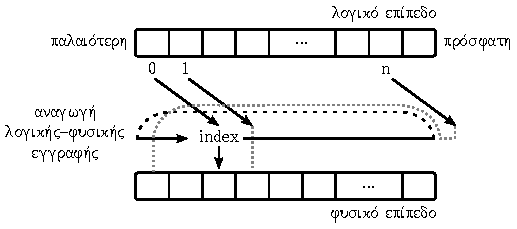
\includegraphics{log_structure}
    \end{center}
\end{figure}


\section{Ώρα συστήματος}
\label{sec:rtc}

Η υλοποίηση περιλαμβάνει τη χρήση ενός ολοκληρωμένου ως ρολόι πραγματικού χρόνου
(\te{Real-Time Clock - RTC}), το DS1307, το οποίο παρέχει ημερομηνία και ώρα
μέχρι δευτερολέπτων, χαρακτηρίζεται από καλή ακρίβεια (απώλεια μερικών
δευτερολέπτων το μήνα), χαμηλή κατανάλωση ισχύος και δυνατότητα διατήρησης της
λειτουργίας του με εφεδρική τροφοδοσία (μέσω μπαταρίας).

Το RTC διαθέτει 7 καταχωρητές για την ημερομηνία\slash{}ώρα και έναν για τη
ρύθμιση του παραγόμενου τετραγωνικού παλμού, ενώ ορισμένα bit ελέγχου βρίσκονται
σε ορισμένες θέσεις των καταχωρητών ημερομηνίας\slash{}ώρας
\parencite[8]{ds1307}. Η ημερομηνία\slash{}ώρα
αναπαριστάται με συμβολισμό BCD (\te{packed Binary-Coded Decimal}) σύμφωνα με
τον οποίο κάθε δεκαδικό ψηφίο αποθηκεύεται σε 4bit \parencite[8]{ds1307}.
Για παράδειγμα, ο αριθμός 12 του δεκαδικού συστήματος αρίθμησης αποκτά δυαδική
αναπαράσταση 0001~0002 αντί της συνήθης 0000~1100.

Κατά την αρχική σύνδεση με τη τροφοδοσία, το ρολόι είναι απενεργοποιημένο, κάτι
που σηματοδοτείται από την ένδειξη CH (\te{Clock Halt}) του καταχωρητή 0x00
\parencite[8]{ds1307}. Η επαναφορά του σε 0 ενεργοποιεί το ρολόι και μπορεί να
πραγματοποιηθεί παράλληλα με την αρχική ενημέρωση της ημερομηνίας\slash{}ώρας.

Η επικοινωνία του RTC με το μικροελεγκτή πραγματοποιείται μέσω διαύλου
I\tsup{2}C (\te{Inter-Integrated Circuit}) σύμφωνα με τον οποίο ο μικροελεγκτής
(\te{master} του διαύλου) αποστέλλει το \te{bit START} ακολουθούμενο από τη
διεύθυνση του RTC (στην προκειμένη, 0x68) και το bit πρόθεσης R\slash\nbar{W}
(βλ. \nameref{subsec:i2c} σ.~\pageref{subsec:i2c}) \parencite[1,10]{ds1307}.

\begin{figure}
    \caption{Παράδειγμα εγγραφής και ανάγνωσης από διεύθυνση του RTC.
    \label{fig:rtc:start-r}}
    \begin{center}
    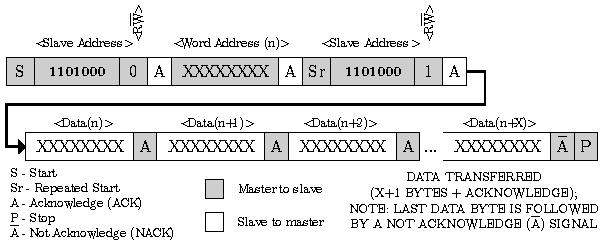
\includegraphics{ds1307_start-r}
    \end{center}
    \fullcite[13]{ds1307:start-r}
\end{figure}

Κατόπιν, ακολουθεί η διεύθυνση του καταχωρητή προς ανάγνωση\slash{}εγγραφή (του
RTC) και το επιθυμητό πλήθος Byte. Σαφώς, παρεμβάλλονται τα \te{bit} ACK μετά
την κάθε επιτυχούσα παραλαβή Byte. Το σχήμα \ref{fig:rtc:start-r} παρουσιάζει
την αποστολή της επιθυμητής διεύθυνσης του RTC (\te{Word Address (n)}), την
επανεκκίνηση της επικοινωνίας (Sr) σε λειτουργία ανάγνωσης και την παραλαβή ενός
πλήθους Byte από το RTC. Σημειώνεται ότι το RTC DS1307 υποστηρίζει ανάγνωση%
\slash{}εγγραφή σε \te{burst mode}, σύμφωνα με την οποία ο εσωτερικός δείκτης
της επιθυμητής διεύθυνσης αυξάνεται αυτόματα με τη διεκπεραίωση κάθε Byte
\parencite[12]{ds1307}.


\subsection{Μνήμη RAM}
\label{subsec:rtc:user-ram}

Το RTC DS1307 διαθέτει κοινόχρηστη μνήμη 56Byte η οποία διατηρεί τα δεδομένα της
ακόμα και όταν το RTC μεταπίπτει στην εφεδρική τροφοδοσία (μπαταρία)
\parencite[1]{ds1307}. Το χαρακτηριστικό αυτό είναι ιδιαίτερα χρήσιμο, καθώς η
μνήμη του μπορεί να χρησιμοποιηθεί για την αποθήκευση ρυθμίσεων της συσκευής που
διατηρούνται μεταξύ διαδοχικών αποσυνδέσεών της από την κύρια τροφοδοσία που,
ωστόσο, είναι εύκολο να αναιρεθούν με την προσωρινή αποσύνδεση της μπαταρίας από
τη συσκευή (προκαλώντας επαναφορά στις εργοστασιακές της ρυθμίσεις) (βλ.
\nameref{subsec:backup-memory} σ.~\pageref{subsec:backup-memory}).

Οι διευθύνσεις της μνήμης έπονται των καταχωρητών (διεύθυνση 0x08) και
εκτείνονται μέχρι την 0x3F \parencite[8]{ds1307}.

%\subsection{Συνδεσμολογία}
% XTAL frequency, ground plane


\section{Ανάθεση εργασιών}
\label{sec:task}

Στο κεφάλαιο του υποσυστήματος κίνησης (σ.~\pageref{ch:motor})
παρουσιάζεται ο υποκείμενος μηχανισμός για τον έλεγχο της κίνησης της κεφαλής
της συσκευής.
Ωστόσο, στο πλαίσιο της υλοποίησης, η χρήση του υποσυστήματος κίνησης είναι
άρρηκτα συνδεδεμένη με την πραγματοποίηση μετρήσεων· η κεφαλή μετακινείται σε
μία
θέση με σκοπό τη δειγματοληψία και καταχώρηση της μέτρησης των αισθητήρων για
εκείνο το σημείο του υλικού. Αυτή η πρόσθετη λειτουργία παρέχεται από ξεχωριστό
τμήμα, τη μονάδα εργασίας (\te{task}).


\subsection{Εργασία δειγματοληψίας}

Η πραγματοποίηση μίας εργασίας για τη δειγματοληψία του μέσου μπορεί να
περιγραφεί από τα ακόλουθα στάδια:
\begin{enumerate}
    \item Μετατόπιση κεφαλής σε νέο ζεύγος συντεταγμένων XY.
    \item Διείσδυση της κεφαλής στο παρακολουθούμενο μέσο.
    \item Λήψη μέτρησης των αισθητήρων και καταχώρησή τους στο Ημερολόγιο
    (σ.~\pageref{sec:log}).
    \item Ανύψωση της κεφαλής.
\end{enumerate}

Δεδομένου ότι η κεφαλή βρίσκεται ανυψωμένη (προεπιλεγμένη θέση κατόπιν
παλιννόστησης) (βλ. σ.~\pageref{subsec:motor:homing}),
τα δύο πρώτα στάδια πραγματοποιούνται αυτόματα από τον
υποκείμενο μηχανισμό. Κατά την ολοκλήρωση της μετατόπισης της κεφαλής
(συμπεριλαμβανομένης και της διείσδυσής στο μέσο), το υποσύστημα κίνησης
ενημερώνει για το συμβάν (μέσω επανάκλησης) το υποσύστημα εργασίας (ή όποιο άλλο
του έχει δηλωθεί).

Στο σημείο αυτό, η μονάδα εργασίας αναλαμβάνει το 3\tsup{ο} στάδιο. Κατόπιν,
προκαλεί την ανύψωση της κεφαλής, η οποία εκτελείται ασύγχρονα (όπως συμβαίνει,
άλλωστε, με κάθε κίνηση της κεφαλής). Η μονάδα εργασίας ειδοποιείται ξανά
όταν η κεφαλή έχει επανατοποθετηθεί στην κορυφαία της θέση. Πλέον, εφόσον
απαιτείται, είναι δυνατό να δρομολογηθεί μία νέα μέτρηση προκαλώντας τη
μετατόπιση της κεφαλής σε νέες συντεταγμένες XYZ με $\text{Z} = 0$, ώστε το
υποσύστημα εργασίας να ειδοποιηθεί όταν η κεφαλή βρίσκεται σε θέση για νέα
δειγματοληψία.

Στο σχήμα \ref{fig:task:samples} παρουσιάζεται πώς το υποσύστημα εργασίας
προκαλεί την αρχική ενεργοποίηση τους υποσυστήματος κίνησης (για τη μετακίνηση
σε νέα θέση) και πώς οι διαδοχικές διεκπεραιώσεις της μετακίνησης της κεφαλής
οδηγούν, σταδιακά, στην ολοκλήρωση του ανατεθειμένου πλήθους μετρήσεων. Η
ενεργοποίηση της εργασίας παραλείπεται το σχήμα, εσκεμμένα, και ο λόγος
περιγράφεται στην \nameref{ssubsec:task:initiate}
(σ.~\pageref{ssubsec:task:initiate}).

\begin{figure}
    \caption{Σταδιακή ολοκλήρωση φόρτου εργασίας μετρήσεων.
    \label{fig:task:samples}}
    \begin{center}
    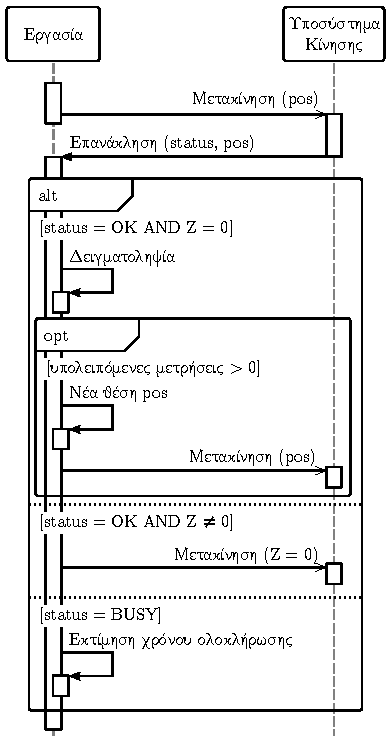
\includegraphics{task_samples}
    \end{center}
\end{figure}

Ένα αναγκαίο στοιχείο για την πραγματοποίηση πολλαπλών μετρήσεων είναι η ύπαρξη
ενός μηχανισμού για την παραγωγή νέων, προς δειγματοληψία, θέσεων. Ένας τέτοιος
μηχανισμός θα μπορούσε να λαμβάνει υπόψη προηγούμενες μετρήσεις ώστε να
προτιμώνται τοποθεσίες που έχουν καιρό να υποστούν εξέταση ή εκείνες στις οποίες
είχαν εντοπιστεί κρίσιμες τιμές. Ωστόσο, στο πλαίσιο της υλοποίησης, ο
μηχανισμός αρκείται στην παραγωγή τυχαίων θέσεων που βασίζονται, ελαφρώς, στην
τρέχουσα ημέρα και ώρα της συσκευής
% \nref : RTC
και στην τρέχουσα θέση της κεφαλής.


\subsubsection{Εκτιμώμενος χρόνος ολοκλήρωσης}

Στο σχήμα \ref{fig:task:samples} γίνεται αναφορά σε εκτίμηση του χρόνου
ολοκλήρωσης η οποία εκτελείται όποτε η επανάκληση αναφέρει ότι το υποσύστημα
κίνησης είναι απασχολημένο (\te{BUSY}). Ο λόγος ύπαρξης του μηχανισμού εκτίμησης
είναι η
παροχή μίας ένδειξης του χρόνου για τον οποίο το υποσύστημα κίνησης, καθώς και
όλες οι λειτουργίες που βασίζονται σε αυτόν, είναι αδύνατο να χρησιμοποιηθούν
έως ότου παρέλθει. Χαρακτηριστική περίπτωση χρήσης του εκτιμώμενου χρόνου είναι
στο πεδίο κεφαλίδας HTTP \te{Retry-After} κατά τις αποκρίσεις με κωδικούς
κατάστασης 202 και 503 (βλ. \nameref{sec:network:impl-resources}
σ.~\pageref{sec:network:impl-resources}).

Όπως αναφέρεται στο Υποσύστημα Κίνησης
(σσ.~\pageref{ssubsec:motor:routing},%
\pageref{ssubsec:motor:common-translation}),
η μετατόπιση της κεφαλής σε νέα θέση πραγματοποιείται σε τρία, το πολύ, στάδια·
κοινή μετατόπιση στο επίπεδο X-Y, υπολειπόμενη μετατόπιση σε άξονα X ή Υ και
μετατόπιση σε άξονα Z ή, εναλλακτικά, πρώτα η μετατόπιση στον άξονα Z και μετά
των άλλων δύο. Πριν την εκκίνηση κάθε σταδίου, και ενώ οι κινητήρες
βρίσκονται σε ηρεμία, αναγγέλλεται από το υποσύστημα κίνησης (μέσω της
επανάκλησης) ο νέος προορισμός και η αλλαγή της κατάστασής του σε \te{BUSY}. Η
πληροφορία αυτή σε συνδυασμό το υπολειπόμενο πλήθος μετρήσεων μπορεί να
χρησιμοποιηθεί για την εκτίμηση της συνολικής διάρκειας της εργασίας.

\begin{figure}
    \caption{Στάδια περάτωσης μίας εργασίας μέτρησης.
    \label{fig:task:estimate-update}}
    Οι στιγμές αναγγελίας \te{BUSY} (βέλη) αποτελούν τα σημεία όπου ανανεώνεται
    η εκτίμηση του χρόνου ολοκλήρωσης. Ο αστερίσκος (*) δηλώνει μία ενδεχόμενη
    πρόσθετη αναγγελία, εφόσον υπολείπεται κίνηση σε έναν εκ των δύο αξόνων X ή
    Y.
    \begin{center}
    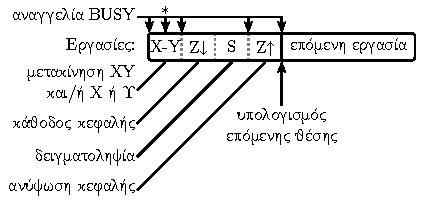
\includegraphics{task_estimate-update}
    \end{center}
\end{figure}

Το σχήμα \ref{fig:task:estimate-update} παρουσιάζει τις συνιστώσες της εργασίας
καθώς και τις στιγμές που αναγγέλλεται η ολοκλήρωση ενός μέρους της μετατόπισης
(σημεία \te{BUSY}). Στο σχήμα, στην περίπτωση της μετατόπισης στο επίπεδο X-Y,
σημειώνεται μία ενδεχόμενη δεύτερη αναγγελία (με αστερίσκο) όταν
πραγματοποιείται ξεχωριστή μετατόπιση σε έναν εκ των δύο αξόνων για το
υπολειπόμενο πλήθος βημάτων. Η λεπτομέρεια αυτή είναι αδιάφορη για τη μονάδα
εργασίας, καθώς αυτό που ενδιαφέρει σε σχέση με το επίπεδο X-Y, είναι η μέγιστη
μετατόπιση μεταξύ των δύο αξόνων.

Όπως αναφέρεται προηγουμένως, η νέα θέση της κεφαλής στο επίπεδο X-Y
υπολογίζεται τη στιγμή ολοκλήρωσης της προηγούμενης εργασίας. Αυτή η σχεδιαστική
επιλογή καθιστά αδύνατο τον ακριβή υπολογισμό του χρόνου ολοκλήρωσης του συνόλου
των εργασιών καθώς οι θέσεις που, τελικά, θα προκύψουν είναι άγνωστες σε
προγενέστερη στιγμή της εκτέλεσης.

Για το λόγο αυτό χρησιμοποιείται ένας αναμενόμενος χρόνος μετατόπισης της
κεφαλής στο επίπεδο X-Y για τις υπολειπόμενες εργασίες ο οποίος, όσο μεγαλύτερο
το πλήθος εργασιών, τόσο μεγαλύτερη απόκλιση από τον πραγματικό χρόνο που
τελικά θα απαιτηθεί. Ωστόσο, καθώς ολοκληρώνονται τα επιμέρους στάδια κάθε
εργασίας και πραγματοποιείται νέα εκτίμηση (σημεία αναγγελίας \te{BUSY}), ο
εκτιμώμενος χρόνος γίνεται ολοένα πιο έγκυρος. Η απόκλιση της εκτίμησης του
χρόνου ολοκλήρωσης της τελευταίας εργασίας κυμαίνεται στα 2, περίπου,
δευτερόλεπτα, μετρική αποδεκτή για τις απαιτήσεις της υλοποίησης.

Η εκτίμηση του χρόνου ολοκλήρωσης του φόρτου εργασίας καθώς και η ώρα κατά την
οποία πραγματοποιήθηκε η εκτίμηση, διατηρούνται. Όποτε προκύπτει ανάγκη για την
επιστροφή του αναμενόμενου χρόνου ολοκλήρωσης ξεκινώντας κάποια δεδομένη χρονική
στιγμή, αρκεί να αφαιρεθεί από εκείνη την ώρα, η ώρα της τελευταίας εκτίμησης
και να συγκριθεί το αποτέλεσμα με την εκτίμηση χρόνου για να διαπιστωθεί πόσος
εκτιμημένος χρόνος έχει παρέλθει.


\subsubsection{Εκκίνηση εργασίας}
\label{ssubsec:task:initiate}

Η δειγματοληψία του μέσου είναι δυνατό να ξεκινήσει με δύο τρόπους· κατόπιν
προτροπής εξωτερικής οντότητας ή από το ίδιο το σύστημα υπό τις κατάλληλες
συνθήκες. Η εκκίνηση εργασιών από εξωτερική οντότητα περιγράφεται στη μέθοδο
\te{POST} του πόρου μετρήσεων του διακομιστή
(σ.~\pageref{ssubsec:network:measurement-post}) και παρέχεται κυρίως για λόγους
εξακρίβωσης λειτουργίας.

Η κύρια πηγή εκκίνησης των κύκλων εργασιών παραμένει το ίδιο το σύστημα.
Για το σκοπό αυτό, κρίνεται
αρκετή η τήρηση της ώρας της πιο πρόσφατης μέτρησης και μίας ένδειξης για το
ελάχιστο επιθυμητό διάστημα μεταξύ διαδοχικών κύκλων εργασίας. Επίσης,
απαιτείται η ύπαρξη ενός ελέγχου για την εξακρίβωση του χρόνου που έχει παρέλθει
από την πλέον πρόσφατη μέτρηση μέχρι τη στιγμή που πραγματοποιείται ο έλεγχος.

Προφανώς, η ημερομηνία της πλέον πρόσφατης μέτρησης τίθεται κατά την
αρχικοποίηση της συσκευής (\te{power-on}) βάσει της τελευταίας καταχωρημένης
εγγραφής του ημερολογίου και ενημερώνεται με κάθε νέα πραγματοποιηθείσα μέτρηση.

Ωστόσο, στην πραγματικότητα, ο μηχανισμός βασίζεται στη χρήση χρονοσφραγίδων που
αντιπροσωπεύουν τα λεπτά που έχουν παρέλθει από την αρχή της ημέρας για κάθε
ημερομηνία. Για την ακρίβεια, επιλέγεται η ημέρα να χωρίζεται σε 240 κβάντα, ενώ
κάθε χρονοσφραγίδα προσδιορίζει κάποια στιγμή της ημέρας ως ένα πλήθος τέτοιων
κβάντων. Όποτε προκύπτει ανάγκη για τον έλεγχο του χρονικού διαστήματος που έχει
παρέλθει μεταξύ πρόσφατης και τρέχουσας ώρας, η τρέχουσα ώρα ανάγεται σε
χρονοσφραγίδα (δηλαδή, σε κβάντα των 6 λεπτών) και συγκρίνεται με τη
χρονοσφραγίδα της μέτρησης (σχήμα \ref{fig:task:interval}).

\begin{figure}
    \caption{Αντιστοίχηση ωρών σε κβάντα και υπολογισμός χρονικού διαστήματος.
    \label{fig:task:interval}}
    Με n συμβολίζεται η κάθε ώρα της ημέρας και κυμαίνεται μεταξύ 0 και 23, ενώ
    για κάθε ώρα ορίζονται 10 κβάντα. Συνολικά, μία μέρα διαθέτει 240 κβάντα.
    \begin{center}
    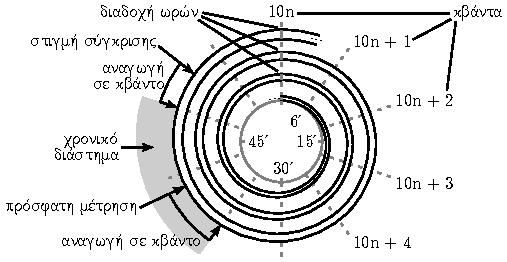
\includegraphics{task_interval}
    \end{center}
\end{figure}

Ο υπολογισμός της χρονοσφραγίδας είναι απλός· οι ώρες μετατρέπονται σε λεπτά και
χωρίζονται σε κβάντα, κατόπιν, προστίθεται η αξία (ευκλείδεια διαίρεση) των
λεπτών σε κβάντα, ως εξής:
\begin{equation}
Q = \frac{60 hrs + min}{q}
\end{equation}
, όπου $q$ η αξία κάθε κβάντου σε λεπτά ($q = 6$).

Ως άμεσο αποτέλεσμα, είναι δυνατή η διάκριση των ωρών με ακρίβεια το πολύ 6
λεπτών. Επιπλέον, η τήρηση μέχρι 240 κβάντων (δηλαδή, μίας ημέρας) συνεπάγεται
ότι οι δύο ημερομηνίες συγκρίνονται μόνο ως προς τις ώρες και τα λεπτά,
αγνοώντας τη διαφορά τους σε ημέρες, μήνες και έτη. Τυπικά, το πρόβλημα αυτό
είναι αμελητέο καθώς η σύγκριση των χρονοσφραγίδων πραγματοποιείται κάθε λίγα
δευτερόλεπτα. Μόνο στην περίπτωση παρατεταμένης διακοπής της τροφοδοσίας του
ρεύματος ενδέχεται να εμφανιστεί κάποια ασυνέχεια με τη μορφή καθυστερημένης
εκκίνησης του επόμενου κύκλου εργασίας που οφείλεται στο ότι η συσκευή αναμένει
να παρέλθει το καθορισμένο πλήθος κβάντων από την τελευταία \emph{ώρα} μέτρησης,
ανεξαρτήτως της ημέρας κατά την οποία πραγματοποιήθηκε.


\subsubsection{Περιοδικός έλεγχος}

Είναι σαφές ότι ο έλεγχος της χρονοσφραγίδας απαιτεί ένα έναυσμα που να προκαλεί
την εκτέλεσή του. Επίσης, θα πρέπει να είναι ικανό να αφυπνίζει τη μονάδα
επεξεργασίας από λειτουργία χαμηλής κατανάλωσης που αυτή τίθεται όσο αναμένει
κάποια νέα εργασία. Σύμφωνα με το εγχειρίδιο της \textcite[38]{atmel13}, ο
χρονομετρητής WDT (\te{Watchdog Timer}) μπορεί να χρησιμοποιηθεί για την
αφύπνιση της MCU από οποιαδήποτε λειτουργία χαμηλής κατανάλωσης.

Ο χρονομετρητής WDT χρησιμοποιεί παλμούς ανεξάρτητου ταλαντωτή και ρυθμίζεται
για περιοδική ενεργοποίηση (μέσα από ένα εύρος πιθανών περιόδων) κατά την οποία
προκαλεί διακοπή ή ακόμα και επανεκκίνηση του μικροελεγκτή (\te{reset})
\parencite[50]{atmel13}. Το δεύτερο είναι ιδιαίτερα σημαντικό για την αποφυγή
ατερμόνων βρόχων αλλά απαιτεί την, από λογισμικού, επανέναρξη του μετρητή πριν
την πρόκληση της επανεκκίνησης \parencite[50]{atmel13}.

Στο πλαίσιο της υλοποίησης, ο WDT ρυθμίζεται μόνο για την αναγγελία διακοπής, η
οποία είτε αφυπνίζει την MCU και εκτελεί τη ρουτίνα εξυπηρέτησης της, είτε
αναμένει την ολοκλήρωση κάποιας άλλης ρουτίνας (για παράδειγμα, την απόκριση σε
κάποιο εισερχόμενο αίτημα HTTP) πριν εκτελεστεί η ίδια για την εκκίνηση του
επόμενου κύκλου εργασίας, εφόσον απαιτείται. Σημειώνεται ότι ο επιλεγμένος
μικροελεγκτής (ATmega328P), υποστηρίζει περιόδους από 16ms μέχρι 8s
\parencite[55]{atmel13}.


\subsection{Μέτρηση θερμοκρασίας}
\label{subsec:ds18b20}

%Συνολικά, απαιτούνται τρία αισθητήρια όργανα για την κάλυψη των βασικών αναγκών
%του συστήματος· θερμοκρασία, υγρασία και οξύτητα.
Στο παρόν στάδιο της υλοποίησης, μόνο η μελέτη και διασύνδεση με τον αισθητήρα
θερμοκρασίας υλοποιείται.
Η μέτρηση της θερμοκρασίας αναλαμβάνεται από ψηφιακό θερμόμετρο, το ολοκληρωμένο
DS18B20, το οποίο βρίσκεται ενσωματωμένο σε στεγανό σωληνάριο και προσαρτημένο
στην κινητή κεφαλή της συσκευής ώστε καθώς αυτή κινείται να επιτρέπεται η
μεταφορά του γύρω και εντός του παρακολουθούμενου υλικού. Το επιλεγμένο
ολοκληρωμένο χαρακτηρίζεται από ακρίβεια $\pm0.5^\circ$C σε θερμοκρασία
λειτουργίας $-55$ έως $+125^\circ$C, διασύνδεση 1-Wire (βλ. σ.~%
\pageref{subsec:1-wire}) με δυνατότητα τροφοδοσίας από τη (μοναδική) γραμμή του
διαύλου με ρυθμιζόμενη ακρίβεια από 9 έως 12bit \parencite[1]{ds18b20}.

\begin{figure}
    \caption{Πτητική μνήμη (\te{scratchpad}) και μνήμη EEPROM του DS18B20.
    \label{fig:ds18b20:memories}}
    \begin{center}
    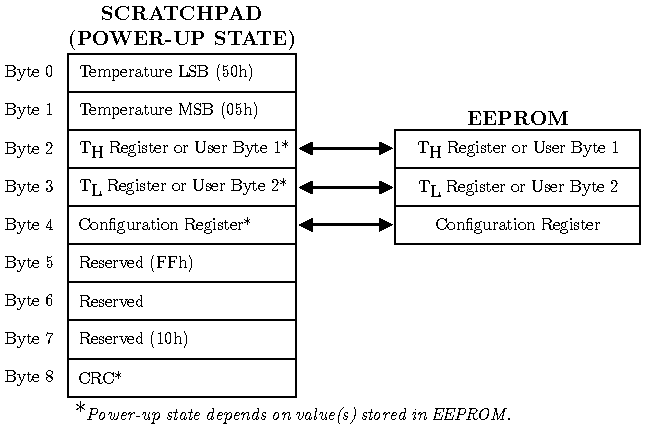
\includegraphics{ds18b20_memories}
    \end{center}
    Βασισμένο \fullcite[7]{ds18b20:memories}
\end{figure}


\subsubsection{Καταχωρητές DS18B20}
\label{ssubsec:ds18b20:registers}

Η μνήμη του αποτελείται από 9Byte με πλέον σημαντικά, για τις ανάγκες της
υλοποίησης, τα δύο πρώτα, στα οποία εναποτίθεται η μέτρηση της θερμοκρασίας.
Ακολουθούν δύο καταχωρητές που προσδιορίζουν δύο όρια θερμοκρασιών τα οποία αν
ξεπεραστούν από κάποια μέτρηση, θέτουν σχετική ένδειξη στην εσωτερική κατάσταση
του ολοκληρωμένου, η οποία μπορεί να χρησιμοποιηθεί για τη συμμετοχή στη
διαδικασία επιλογής \te{slave} συσκευής, μόνο εκείνων των ολοκληρωμένων που
χρήζουν άμεσης ανάγκης \parencite[4--5]{ds18b20}. Προφανώς, συγκρίνεται μόνο το
ακέραιο τμήμα της θερμοκρασίας με την τιμή των καταχωρητών καθώς οι καταχωρητές
είναι του 1Byte ο καθένας (βλ. και σχήμα \ref{fig:ds18b20:t-format}). Η σχετική
εντολή ROM ονομάζεται \te{ALARM SEARCH}. Εναλλακτικά, μπορούν να χρησιμοποιηθούν
για την αποθήκευση δεδομένων της συσκευής που, σε συνδυασμό με την εντολή
\te{COPY SCRATCHPAD} (βλ. παρακάτω), διατηρούνται μεταξύ διαδοχικών αποσυνδέσεων
της συσκευής από την τροφοδοσία.

Ο καταχωρητής στη διεύθυνση 4 καθορίζει την ακρίβεια και, συνεπώς το χρόνο που
απαιτεί κάθε μέτρηση \parencite[4,8]{ds18b20}. Υποστηρίζεται ακρίβεια των 12 έως
9bit, με κάθε μικρότερη να απορρίπτει ένα μέρος του κλάσματος της μέτρησης.

Τα Byte 5 έως 7 χρησιμοποιούνται για τις ανάγκες του ολοκληρωμένου, ενώ στο Byte
8 υπολογίζεται το αποτέλεσμα του πολυωνύμου για την επιβεβαίωση της εγκυρότητας
των δεδομένων κατά την ανάγνωσή τους από το \te{master}.

Η μορφή με την οποία αποθηκεύεται η θερμοκρασία στους δύο πρώτους καταχωρητές
παρουσιάζεται στο σχήμα \ref{fig:ds18b20:t-format}. Η θερμοκρασία αποθηκεύεται
με πρόσημο ως συμπλήρωμα του 2 \parencite[3]{ds18b20}. Στο πλαίσιο της
υλοποίησης, αυτοί είναι οι μοναδικοί καταχωρητές του DS18B20 που αξιοποιούνται.

\begin{figure}
    \caption{Μορφή θερμοκρασίας στους καταχωρητές 0 και 1 του DS18B20.
    \label{fig:ds18b20:t-format}}
    \begin{center}
    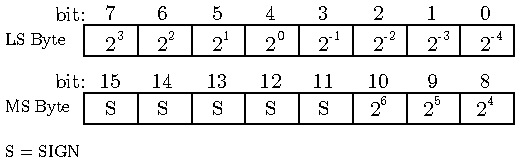
\includegraphics{ds18b20_t-format}
    \end{center}
    Βασισμένο \fullcite[4]{ds18b20:t-format}
\end{figure}

\subsubsection{Υποστηριζόμενες εντολές}
\label{ssubsec:ds18b20:commands}

Στην ενότητα \nameref{subsec:1-wire} (σ.~\pageref{subsec:1-wire}) περιγράφεται η
έννοια της συναλλαγής κατά την οποία πραγματοποιείται αρχικοποίηση, ακολουθεί η
επιλογή μία συσκευής \te{slave} μέσω εντολών ROM και, τελικά, αποστέλλεται η
εντολή λειτουργίας (\te{Function command}) που είναι επιθυμητό να εκτελεστεί.
Στην περίπτωση του DS18B20, οι υποστηριζόμενες εντολές λειτουργίας είναι οι
ακόλουθες:
\begin{description}
    \item[CONVERT T [0x44{]}] Προκαλεί την λήψη μίας νέας μέτρησης. Σε περίπτωση
    που η τροφοδοσία του ολοκληρωμένου είναι ανεξάρτητη από τη γραμμή του
    διαύλου, η ολοκλήρωση σηματοδοτείται από την απελευθέρωση της γραμμής από
    το DS18B20 και την επαναφορά του σε λογικό 1 από τον αντιστάτη \te{pull-up}
    \parencite[11]{ds18b20}. Σε αντίθετη περίπτωση, ο μικροελεγκτής είναι
    υποχρεωμένος να αποφασίσει πόσο χρόνο να αναμείνει ώστε να ολοκληρωθεί η
    μετατροπή, με μέγιστο 750ms για ακρίβεια 12bit \parencite[8,11]{ds18b20}.

    \item[WRITE SCRATCHPAD [0x4E{]}] Επιτρέπει την αποστολή τριών Byte που
    εναποτίθενται στις διευθύνσεις 2, 3 και 4 της πτητικής μνήμης του
    ολοκληρωμένου (καταχωρητές T\tsub{H}, T\tsub{L} και ρυθμίσεων)
    \parencite[11]{ds18b20}.

    \item[READ SCRATCHPAD [0xBE{]}] Επιτρέπει την πλήρη ή μερική ανάγνωση της
    πτητικής μνήμης του ολοκληρωμένου ξεκινώντας από το λιγότερο σημαντικό
    \te{bit} του Byte 0, διαδοχικά εκτεινόμενη προς στις επόμενες θέσεις
    \parencite[11]{ds18b20}.

    \item[COPY SCRATCHPAD [0x48{]}] Μεταφέρει τα Byte T\tsub{H}, T\tsub{L} και
    ρυθμίσεων (Byte 2, 3 και 4, αντιστοίχως) από την πτητική μνήμη του DS18B20
    στη μνήμη EEPROM ώστε να διατηρούνται μεταξύ διαδοχικών αποσυνδέσεων του
    ολοκληρωμένου \parencite[12]{ds18b20}.

    \item[RECALL E\protect\tsup{2} [0xB8{]}] Επαναφέρει τα Byte 2, 3 και 4 από
    τη μνήμη EEPROM στην πτητική μνήμη του DS18B20 \parencite[12]{ds18b20}.

    \item[READ POWER SUPPLY [0xB4{]}] Επιτρέπει στο \te{master} να αναγνωρίσει
    εάν το ολοκληρωμένο τροφοδοτείται μέσω του ακροδέκτη V\tsub{CC} ή εάν
    βασίζεται στη γραμμή του διαύλου \parencite[12]{ds18b20}.
\end{description}

\begin{figure}
    \caption{Συναλλαγές 1-Wire για τη δειγματοληψία της θερμοκρασίας.
    Στην υλοποίηση, χρησιμοποιείται μόνο το DS18B20 ως \te{slave} συσκευή με
    αποτέλεσμα να μην απαιτείται η ρητή αναγγελία του αναγνωριστικού του, και
    για αυτό χρησιμοποιείται η εντολή SKIP ROM. Με DQ συμβολίζεται η κατάσταση
    της γραμμής του διαύλου 1-Wire, ενώ ο τερματικός Παλμός \te{Reset} θα
    μπορούσε, κάλλιστα, να ανήκει σε επόμενο ζεύγος παλμών αρχικοποίησης
    (βλ. σ.~\pageref{ssubsec:1-wire:initialisation}).
    \label{fig:ds18b20:sample}}
    \begin{center}
    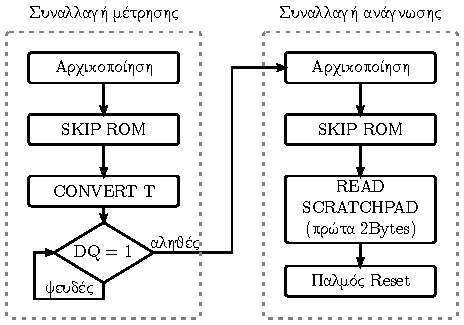
\includegraphics{ds18b20_sample}
    \end{center}
\end{figure}

Στο πλαίσιο της υλοποίησης, οι εντολές που χρησιμοποιούνται είναι οι \te{CONVERT
T} και \te{READ SCRATCHPAD}. Μία τυπική επικοινωνία μεταξύ του μικροελεγκτή και
του DS18B20 απεικονίζεται στο σχήμα \ref{fig:ds18b20:sample} κατά την οποία
πραγματοποιούνται δύο συναλλαγές, μία για την εκκίνηση της μέτρησης και μία για
την ανάγνωση της μνήμης και, για την ακρίβεια, των δύο πρώτων καταχωρητών που
αντιστοιχούν στη μέτρηση. Αυτό είναι δυνατό να επιτευχθεί αποστέλλοντας τον
παλμό \te{Reset} αμέσως μετά την ανάγνωση του δεύτερου \te{Byte}.

Όπως παρουσιάζεται στο σχήμα, η επιλογή του DS18B20 γίνεται μέσω της εντολής
\te{SKIP} ROM η οποία, στην πραγματικότητα, παραλείπει την αναγγελία
αναγνωριστικού και μεταβαίνει, απευθείας, στην αποστολή εντολής λειτουργίας
(\te{Function command}). Η συγκεκριμένη τακτική μπορεί να χρησιμοποιηθεί υπό την
προϋπόθεση ότι το DS18B20 είναι το μοναδικό ολοκληρωμένο που συνδέεται στο
δίαυλο 1-Wire, κάτι που ισχύει για την υλοποίηση. Σε αντίθετη περίπτωση, η
επιλογή περισσότερων ολοκληρωμένων θα προκαλούσε σύγκρουση κατά την ανάγνωση της
μέτρησης όπου ταυτόχρονα θα επιχειρούσαν να αναγγείλουν τα \te{bit} τους.

Τέλος, αναφέρεται ότι κατόπιν υποβολής της εντολής μέτρησης της θερμοκρασίας, ο
μικροελεγκτής αναμένει την απελευθέρωση (και επαναφορά σε λογικό 1) της γραμμής
του διαύλου από το DS18B20 προκειμένου να προβεί στη συναλλαγή της ανάγνωσης. Η
δυνατότητα αναγγελίας της ολοκλήρωσης με αυτόν τον τρόπο είναι διαθέσιμη, όπως
αναφέρεται παραπάνω, μόνο στην περίπτωση που το DS18B20 τροφοδοτείται μέσω του
ακροδέκτη V\tsub{CC} και όχι μέσω της ίδιας της γραμμής του διαύλου.

Στο πλαίσιο της υλοποίησης επιλέγεται η χρήση του ακροδέκτη V\tsub{CC} για την
τροφοδοσία του DS18B20 για δύο λόγους.
Καταρχήν, για τη τροφοδοσία του ολοκληρωμένου μέσω της γραμμής, η
\textcite[5]{ds18b20} συνιστά τη χρήση ενός ισχυρού στοιχείου για την επαναφορά
της (όπως MOSFET) και όχι μόνο ενός αντιστάτη καθώς κατά την μέτρηση της
θερμοκρασίας, η απότομη αύξηση κατανάλωσης έντασης ρεύματος μπορεί να προκαλέσει
πτώση στην τάση της γραμμής με αποτέλεσμα η εργασία να μην ολοκληρωθεί επιτυχώς.
Με τη σειρά του, η μέθοδος αυτή απαιτεί ένα επιπλέον τρανζίστορ καθώς και την
απόδοση ενός επιπρόσθετου ακροδέκτη του μικροελεγκτή για το σκοπό.

Ο δεύτερος λόγος σχετίζεται με τη μορφή του αισθητήριου οργάνου. Το προϊόν που
χρησιμοποιείται διαθέτει ένα DS18B20 ενσωματωμένο στο ένα άκρο ενός στεγανού
σωληναρίου με τρεις απολήξεις σύνδεσης στο άλλο· V\tsub{CC}, GND και DQ.
Επομένως, ήδη υπάρχει αγωγός για τη σύνδεση του ακροδέκτη V\tsub{CC} με την
τροφοδοσία με αποτέλεσμα η χρήση της γραμμής DQ για την τροφοδοσία να φαντάζει
άσκοπη.


\section{Δίαυλοι επικοινωνίας ολοκληρωμένων}
\label{sec:buses}

Στο πλαίσιο της υλοποίησης, γίνεται χρήση των ακόλουθων διαύλων για την
επικοινωνία του μικροελεγκτή με επιλεγμένα ολοκληρωμένα κυκλώματα:
\begin{description}
    \item[1-Wire] της \te{Dallas Semiconductor}, δίαυλος ασύγχρονης
    ημιαμφίδρομης επικοινωνίας που χρησιμοποιεί μόνο έναν αγωγό (σήμα)
    διασύνδεσης. Χρησιμοποιείται για την επικοινωνία με τον αισθητήρα
    θερμοκρασίας DS18B20. Εφόσον ο μικροελεγκτής αδυνατεί να το υποστηρίξει
    εγγενώς, η υλοποίηση του διαύλου γίνεται εξολοκλήρου σε λογισμικό
    (\te{bit-banging}).

    \item[I\protect\tsup{2}C] της Phillips, δίαυλος σύγχρονης ημιαμφίδρομης
    επικοινωνίας που χρησιμοποιεί δύο αγωγούς σύνδεσης· ένα για συγχρονισμό και
    έναν για δεδομένα. Χρησιμοποιείται για την επικοινωνία με το ρολόι
    πραγματικού χρόνου (RTC) DS1307. Το λογισμικό οδήγησης αξιοποιεί το
    υποκείμενο, και συμβατό, κύκλωμα TWI (\te{Two-Wire Interface}) του
    μικροελεγκτή.

    \item[SPI] ονομασμένο από τη Motorola, δίαυλος σύγχρονης αμφίδρομης
    επικοινωνίας που χρησιμοποιεί τρεις αγωγούς επικοινωνίας -- ρολόι, δεδομένα
    \te{Master} και δεδομένα \te{Slave} -- καθώς και επιπρόσθετη γραμμή επιλογής
    (\nbar{CS}) του εκάστοτε ολοκληρωμένου. Χρησιμοποιείται για την επικοινωνία
    με το ολοκληρωμένο δικτύωσης W5100 και της εξωτερικής μνήμης Flash. Το
    λογισμικό οδήγησης κάθε ολοκληρωμένου αξιοποιεί το υποκείμενο κύκλωμα SPI
    του μικροελεγκτή.
\end{description}

\subsection{Δίαυλος 1-Wire}
\label{subsec:1-wire}

Ο δίαυλος 1-Wire δημιουργήθηκε από την Dallas Semiconductor και για τη
διασύνδεση των συσκευών χρησιμοποιείται μία μόνο γραμμή, η οποία μπορεί να
χρησιμοποιηθεί, υπό περιπτώσεις, και για την τροφοδοσία των συσκευών
επιπροσθέτως της ανταλλαγής δεδομένων \parencite[1]{atmel04}. Η επικοινωνία
είναι ημιαμφίδρομη, ενώ για την αποστολή κάθε \te{bit}, ανεξαρτήτως κατεύθυνσης,
χρησιμοποιούνται χρονοθυρίδες οι οποίες δημιουργούνται από το μοναδικό
\te{master} του διαύλου \parencites[2]{atmel04}[15]{ds18b20}.

\begin{figure}
    \caption{Χρονοθυρίδες εγγραφής και ανάγνωσης στο δίαυλο 1-Wire.
    \label{fig:1-wire:time-slot}}
    \begin{center}
    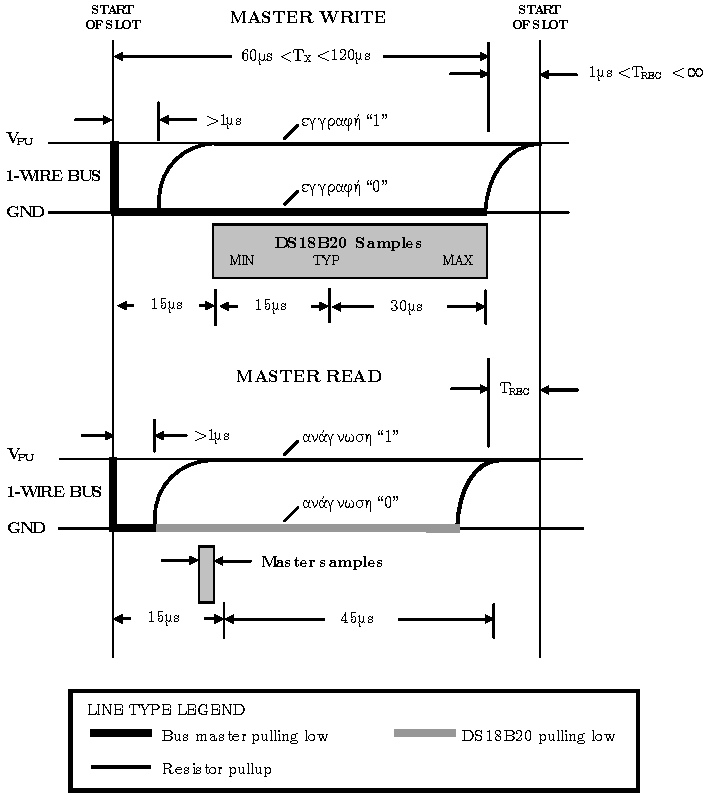
\includegraphics{1-wire_time-slot}
    \end{center}
    Βασισμένο \fullcite[16]{ds18b20:time-slot}
\end{figure}


\subsubsection{Εγγραφή}

Η μορφή των χρονοθυρίδων εμφανίζεται στο σχήμα \ref{fig:1-wire:time-slot}. Σε
περίπτωση εγγραφής ενός \te{bit}, ο \te{master} θέτει τη γραμμή σε λογικό 0 για
1 έως 15μs και, κατόπιν, είτε τη διατηρεί σε αυτήν την κατάσταση αναγγέλλοντας,
με αυτόν τον τρόπο, \te{bit} 0, είτε τίθεται σε κατάσταση υψηλής εμπέδωσης, ώστε
ο αντιστάτης \te{pull-up} να επαναφέρει τη γραμμή σε λογικό 1
\parencite[2]{atmel04}.


\subsubsection{Ανάγνωση}

Για την ανάγνωση ενός \te{bit}, ο \te{master} θέτει τη γραμμή σε λογικό 0
τουλάχιστον για 1μs και, κατόπιν, τίθεται σε κατάσταση υψηλής εμπέδωσης,
δίνοντας τη δυνατότητα στο \te{slave} να αναγγείλει το \te{bit}, ο οποίος, με τη
σειρά του, είτε θέτει τη γραμμή σε λογικό 0, είτε παραμένει σε κατάσταση υψηλής
εμπέδωσης \parencite[2]{atmel04}. Ο \te{master} ελέγχει την κατάσταση της
γραμμής εντός 15μs από την αρχή της χρονοθυρίδας \parencite[17]{ds18b20}
προκειμένου να ανάγει το \te{bit} του \te{slave}.

Είναι εμφανές ότι η ανάγνωση είναι παρόμοια με την εγγραφή \te{bit} τιμής 1·
στην πραγματικότητα, αυτό που διαφοροποιείται είναι η εσωτερική κατάσταση του
\te{slave} που καθορίζει εάν πρόκειται να λάβει ή να εγγράψει κάποιο \te{bit},
όπως, για παράδειγμα, εάν έχει προηγουμένως αποσταλεί εντολή ανάγνωσης κάποιας
διεύθυνσης της μνήμης του.
% \nref : εντολή ανάγνωση μνήμης
Όπως συνιστάται στο εγχειρίδιο της \textcite[17]{ds18b20} και όπως γίνεται ορατό
και στο σχήμα, ο χρόνος κατά τον οποίο η γραμμή παραμένει σε λογικό 0 ως
επενέργεια του \te{master} είναι όσο το δυνατό μικρότερος, ενώ η ανάγνωσή της
γίνεται όσο το δυνατό κοντινότερα στη λήξη του διαστήματος των 15μs. Με αυτόν
τον τρόπο, μειώνεται σημαντικά η πιθανότητα εσφαλμένης ανάγνωσης που οφείλεται
σε μη σταθεροποιημένο σήμα.

Όλες οι χρονοθυρίδες, ανεξαρτήτως εάν πρόκειται για εγγραφή ή ανάγνωση, διαρκούν
από 60 έως 120μs και ακολουθούνται από 1μs, τουλάχιστον, χρόνο ανάκτησης
(T\tsub{REC}) κατά τον οποίο η γραμμή αφήνεται ελεύθερη
\parencites[15--16]{ds18b20}[2]{atmel04}.


\subsubsection{Παλμοί αρχικοποίησης}
\label{ssubsec:1-wire:initialisation}

Η έναρξη της επικοινωνίας μεταξύ \te{master} και \te{slave} γίνεται με την
αποστολή ενός παλμού \te{Reset} από το \te{master} και την απόκριση
του\slash{}των \te{slave} με παλμό \te{Presence} \parencite[15]{ds18b20}. Ο
παλμός \te{Reset} θέτει τη γραμμή σε λογικό 0 τουλάχιστον για 480μs (διάστημα 8
φορές μεγαλύτερο από τις χρονοθυρίδες ανάγνωσης\slash{}εγγραφής), κατόπιν η
γραμμή απελευθερώνεται και εφόσον, εντός 60μs από τη στιγμή εκείνη, η γραμμή
βρίσκεται σε λογικό 0, τότε υπάρχει τουλάχιστον μία συνδεδεμένη \te{slave}
συσκευή στο δίαυλο (παλμός \te{Presence}) \parencite[3]{atmel04}.


\subsubsection{Συναλλαγές}

\begin{figure}
    \caption{Κύκλος συναλλαγής στο δίαυλο 1-Wire.
    \label{fig:1-wire:transaction}}
    Όλες οι συναλλαγές ξεκινούν με τους παλμούς αρχικοποίησης και ακολουθεί η
    επιλογή της επιθυμητής \te{slave} συσκευής και η αποστολή εντολής προς
    αυτήν. Το ακριβές σύνολο εντολών λειτουργίας (\te{Function Command})
    εξαρτάται από την οικογένεια της εκάστοτε συσκευής (για παράδειγμα, λήψη
    θερμοκρασίας από αισθητήρα θερμοκρασίας).
    \begin{center}
    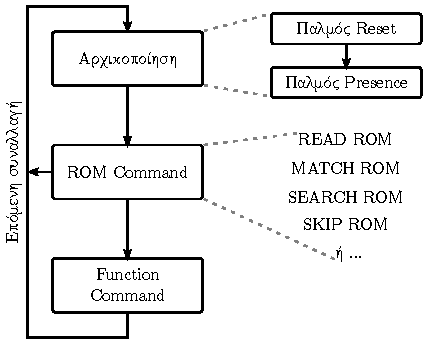
\includegraphics{1-wire_transaction}
    \end{center}
\end{figure}

Στο δίαυλο 1-Wire, εκτός από τους παλμούς αρχικοποίησης και των χρονοθυρίδων
ανάγνωσης\slash{}εγγραφής, ορίζονται ακολουθίες εντολών (δηλαδή, ανταλλαγή
συγκεκριμένων τιμών Byte), αναφερόμενες ως συναλλαγές, για την επίτευξη
οποιασδήποτε λειτουργίας \parencite[10]{ds18b20}. Το σχήμα
\ref{fig:1-wire:transaction} παρουσιάζει τις εργασίες μίας συναλλαγής.
Η αρχικοποίηση έχει περιγραφεί, ενώ οι εντολές λειτουργίας
(\te{Function Command}) εξαρτώνται από τα εκάστοτε είδη των συνδεδεμένων
συσκευών.

\paragraph{Εντολές ROM}%
Ο λόγος ύπαρξης των εντολών ROM αιτιολογείται από την ανάγκη για τον εντοπισμό
και επιλογή μίας συσκευής \te{slave} εκ του συνόλου των συνδεδεμένων στο δίαυλο.
Προκειμένου να είναι αυτό δυνατό, αποδίδεται σε κάθε συσκευή ένα μοναδικό
αναγνωριστικό των 64bit το οποίο περιέχει έναν κωδικό οικογενείας της συσκευής
των 8bit, ένα σειριακό αριθμό των 48bit και κωδικό CRC (\te{Cyclic Redundancy
Check}) των 8bit βάσει των προηγούμενων \te{Byte} \parencite[6]{ds18b20}.
Οι κοινώς υποστηριζόμενες εντολές \te{ROM} είναι οι ακόλουθες:
\begin{description}
    \item[READ ROM [0x33{]}] Επιτρέπει την απευθείας ανάγνωση του
    αναγνωριστικού της μοναδικής \te{slave} συσκευή του διαύλου (δεδομένου ότι
    είναι μόνο μία).

    \item[MATCH ROM [0x55{]}] Για την αναγγελία του επιθυμητού αναγνωριστικού
    των 64bit από το \te{master} και την απόκριση μόνο από το \te{slave} που τον
    διαθέτει. Το συγκεκριμένο μπορεί να χρησιμοποιηθεί εάν, για παράδειγμα,
    είναι, εκ των προτέρων, καταχωρημένα όλα τα πιθανά αναγνωριστικά.

    \item[SEARCH ROM [0xF0{]}] Χρησιμοποιείται για την ανάγνωση των
    αναγνωριστικών των συνδεδεμένων συσκευών, ένα προς ένα, εφόσον τα ακριβή
    στοιχεία τους είναι άγνωστα κατά την εκκίνηση του συστήματος.

    \item[SKIP ROM [0xCC{]}] Παράληψη της επιλογής κάποιας συγκεκριμένης
    συσκευής επειδή πρόκειται να δοθεί η ίδια εντολή σε όλες τις συσκευές ή
    επειδή είναι γνωστό ότι μόνο μία είναι συνδεδεμένη.
\end{description}


\subsubsection{ATmega328P και 1-Wire}

Στο μικροελεγκτή ATmega328P, ο δίαυλος 1-Wire είναι δυνατό να υποστηριχθεί εξ
ολοκλήρου μέσω λογισμικού ή εν μέρει σε λογισμικό και εν μέρει σε υλικό (για
παράδειγμα, USART), χωρίς, ωστόσο, να υπάρχει εγγενώς κάποιο κύκλωμα ειδικά για
αυτόν τον σκοπό \parencite[3]{atmel04}. Στο πλαίσιο της υλοποίησης, επιλέγεται η
πρώτη προσέγγιση (εξ ολοκλήρου σε λογισμικό).

Επιπλέον, δεδομένου ότι χρησιμοποιείται μόνο μία συσκευή (αισθητήρας
θερμοκρασίας), επιλέγεται η μη υλοποίηση της διαδικασίας αναζήτησης \te{slave}
συσκευής (\te{Search ROM}), καθώς η μία που χρησιμοποιείται είναι, εξαρχής,
γνωστή.
% \nref : DS18B20


\subsection{Δίαυλος I\protect\tsup{2}C (TWI)}
\label{subsec:i2c}

%Ο δίαυλος I\tsup{2}C σχεδιάστηκε το 1982 από τη \te{Phillips Semiconductor} με
%αρχικό σκοπό

Βασικά χαρακτηριστικά του διαύλου είναι η διασύνδεση των συσκευών με δύο
γραμμές, τις SDA (\te{Serial DAta}) και SCL (\te{Serial CLock}), τη δυνατότητα
οποιασδήποτε συσκευής να ξεκινήσει την επικοινωνία με κάποια άλλη
(\te{multi-master}) επιλέγοντάς την μέσω μοναδικής διεύθυνσης που διαθέτουν
όλες με συχνότητα του ρολογιού που αναγνωρίζεται από τις ίδιες τις συσκευές
(δεδομένου ότι είναι εντός των επιτρεπτών τους ορίων), χωρίς να απαιτείται
προηγούμενη ρύθμιση κάθε συσκευής ξεχωριστά \parencite[3--4,6]{nxp14}.

Σύμφωνα με την \textcite[6]{nxp14}, προκειμένου κάποια συσκευή να επικοινωνήσει
με κάποια άλλη, απαιτείται πρώτα να αποκτήσει τον έλεγχο του διαύλου (να γίνει
\te{master}). Κατόπιν, αποστέλλει τη διεύθυνση του επιθυμητού \te{slave} (7bit)
ακολουθούμενο από το bit πρόθεσης (λογικό 1 συνεπάγεται ανάγνωση από το
\te{slave}) και λαμβάνει ένα bit επιβεβαίωσης (ACK) από το \te{slave}, σε
περίπτωση επιτυχίας ενώ στη συνέχεια ακολουθούν τα \te{Byte} καθένα συνοδευόμενο
από bit επιβεβαίωσης ή μη \parencite[10,13]{nxp14}.

Σε κατάσταση αδράνειας του διαύλου, οι γραμμές SDA και SCL ηρεμούν σε λογικό 1
μέσω αντιστατών pull-up (αντίστασης, συνήθως, μεταξύ 2--10kΩ) ενώ όλες οι
συνδεδεμένες συσκευές βρίσκονται σε κατάσταση υψηλής εμπέδωσης
\parencites[13]{phillips03}[8]{nxp14}. Σε τυπική λειτουργία, η γραμμή SDA
τίθεται (προετοιμάζεται) όταν η γραμμή SCL βρίσκεται σε λογικό 0. Τη στιγμή που
η SCL ανέρχεται, η SDA θεωρείται ότι έχει σταθεροποιηθεί και οι συνδεδεμένες
συσκευές διαβάζουν την τιμή της. Κατόπιν, η SCL επανέρχεται σε λογικό 0 ώστε η
SDA να τεθεί εκ νέου \parencite[9]{nxp14}.

Επιπλέον, ορίζονται δύο ειδικές περιπτώσεις που χρησιμοποιούνται για την
εκκίνηση και τον τερματισμό της επικοινωνίας από το \te{master} -- η αποστολή
των bit \te{START} και \te{STOP} -- τα οποία αποτελούν τη μεταβολή της SDA σε
λογικό 0 και 1, αντιστοίχως, ενώ η γραμμή SCL βρίσκεται σε λογικό 1
\parencite[9]{nxp14}. Μία υποπερίπτωση αυτών, είναι η αποστολή bit \te{START}
από το \te{master} του διαύλου ώστε να πραγματοποιήσει νέα επικοινωνία (είτε με
την ίδια είτε με άλλη συσκευή) χωρίς να απελευθερώσει το δίαυλο πρώτα το δίαυλο
\parencite[13]{nxp14}. Το bit αυτό αποκαλείται Sr (\te{Repeated Start}) και
είναι ισοδύναμο του bit \te{START} με την εξαίρεση ότι στην περίπτωση που ο
\te{master} λαμβάνει από το \te{slave} πρέπει να αποκριθεί με NACK προτού
αποστείλει το bit Sr \parencite[13--14]{nxp14}.

Ο δίαυλος I\tsup{2}C υποστηρίζει, επίσης, μηχανισμούς διαιτησίας
(\te{arbitration}) και αναγνώρισης συγκρούσεων (\te{collision detection}) που
αξιοποιούνται σε υλοποιήσεις πολλαπλών συσκευών που γίνονται \te{master} του
διαύλου. Στην περίπτωση αυτής της υλοποίησης, \te{master} του διαύλου μπορεί να
είναι μόνο ο μικροελεγκτής και, συνεπώς, αποφεύγεται η περαιτέρω ανάλυσή τους.


%\subsubsection{Two-Wire Interface (TWI)}

Ο μικροελεγκτής της υλοποίησης (ATmega328P) διαθέτει κύκλωμα συμβατό με το
I\tsup{2}C της Phillips υπό το όνομα TWI (\te{Two-Wire Interface}) και δια μέσω
αυτού πραγματοποιείται η διασύνδεσή του με το ολοκληρωμένο
\parencite[209]{atmel13}.

\subsection{Δίαυλος SPI}
\label{subsec:spi}

Η διασύνδεση των συσκευών σε δίαυλο SPI (\te{Serial Peripheral Interface})
γίνεται μέσω τριών, κοινών για όλες τις συσκευές, γραμμών για την ανταλλαγή των
δεδομένων -- SCK (\te{Serial Clock}), MOSI (\te{Master-Out Slave-In}), MISO
(\te{Master-In Slave-Out}) -- και επιπρόσθετων γραμμών για την επιλογή κάθε
\te{slave} συσκευής (\nbar{SS} -- \te{Slave Select})
\parencite[15,24]{motorola04}. Η \te{master} συσκευή είναι υπεύθυνη για την
επιλογή της επιθυμητής, για επικοινωνία, \te{slave} συσκευής καθώς και για την
παραγωγή του ρολογιού, ενώ τα δεδομένα αποστέλλονται ταυτόχρονα και προς τις δύο
κατευθύνσεις \parencite[26--27]{motorola04}.

Στο σχήμα \ref{fig:spi:cpha-0} παρουσιάζονται τα σήματα επικοινωνίας μέσω του
διαύλου SPI. Ο δίαυλος ρυθμίζεται για τη χρήση είτε λογικού 1 είτε 0 ως ενεργό
\te{bit} των παλμών ρολογιού (πολικότητα -- \te{polarity}) καθώς και σε ποια
παρυφή των παλμών του ρολογιού πραγματοποιείται η δειγματοληψία από τις
\te{master} και \te{slave} συσκευές \parencite[27--28]{motorola04}. Στο
παράδειγμα του σχήματος, η δειγματοληψία των γραμμών MOSI και MISO
πραγματοποιείται κατά την μπροστινή παρυφή των παλμών του ρολογιού (για
παράδειγμα, με πολικότητα CPOL = 0, στην ανερχόμενη). Αντιστοίχως, ο δίαυλος
υποστηρίζει τη δειγματοληψία στην οπίσθια παρυφή· η ρύθμιση γίνεται μέσω της
φάσης (\te{Clock Phase}). Οι επιλογές φάσης και πολικότητας ορίζουν τέσσερις
πιθανές ρυθμίσεις λειτουργίας του διαύλου SPI, η εφαρμογής ποιας πρέπει να είναι
εξαρχής γνωστή και προσυμφωνημένη μεταξύ \te{master} και \te{slave}, ενώ είναι
δυνατό να εφαρμόζεται σε κάθε επικοινωνία και μία διαφορετική, σύμφωνα με τις
απαιτήσεις της κάθε συσκευής \parencites[27]{motorola04}[167]{atmel13}.

\begin{figure}
    \caption{Χρονισμός δεδομένων SPI με φάση ρολογιού CPHA = 0.
    \label{fig:spi:cpha-0}}
    \begin{center}
    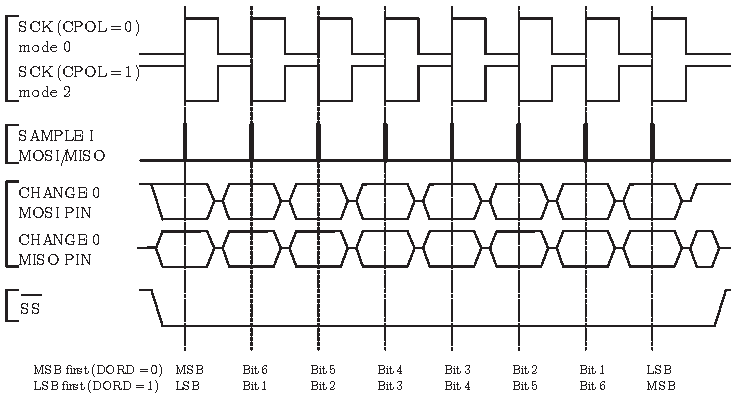
\includegraphics{spi_cpha-0}
    \end{center}
    \fullcite[168]{atmel13:spi-cpha0}
\end{figure}

Ο μικροελεγκτής ATmega238P υποστηρίζει εγγενώς το δίαυλο SPI καθώς διαθέτει
κύκλωμα αφιερωμένο κύκλωμα. Υποστηρίζει και τις τέσσερις ρυθμίσεις λειτουργίας
βάσει συνδυασμού πολικότητας-φάσης με δυνατότητα επιλογής της σειράς αποστολής
των \te{bit} (πλέον ή λιγότερο σημαντικό \te{bit}) ενώ η συχνότητα του ρολογιού
μπορεί να φτάνει μέχρι το μισό της συχνότητας του ρολογιού συστήματος. Οι
επιλογές αυτές γίνονται δια μέσω του καταχωρητή SPCR (\te{SPI Control Register})
\parencite[169]{atmel13}. Παρότι υποστηρίζεται, επιλέγεται η μη αξιοποίηση
διακοπής ως αποτέλεσμα αποστολής\slash{}λήψης κάθε \te{Byte}, αλλά, αντιθέτως, η
αναμονή μέχρι την ενεργοποίηση της ένδειξης SPIF (\te{SPI Interrupt Flag}) του
καταχωρητή SPSR (\te{SPI Status Register}) από το υποκείμενο κύκλωμα
\parencite[167,170]{atmel13}.

Στο πλαίσιο της υλοποίησης, ο δίαυλος SPI χρησιμοποιείται για τη διασύνδεση με
το ολοκληρωμένο δικτυακής σύνδεσης (βλ. \nameref{sec:w5100}
σ.~\pageref{sec:w5100}) και την εξωτερική μνήμη \te{Flash},
ενώ ως λειτουργία χρησιμοποιείται η \te{SPI mode 0} (δηλαδή, CPOL = 0, CPHA = 0)
καθώς υποστηρίζεται και από τα δύο ολοκληρωμένα.

\chapter{Κατασκευή}
\label{ch:construction}

Το κεφάλαιο ασχολείται με την επιλογή και συνδυασμό μηχανικών εξαρτημάτων
προκειμένου να συντεθεί η φυσική υπόσταση της συσκευής (\te{hardware}), η οποία
προορίζεται να ελέγχεται από το λογισμικό του μικροελεγκτή.

Το σημαντικότερο στοιχείο της συσκευής είναι η κεφαλή, η οποία πρόκειται για ένα
όργανο που κινείται σε επίπεδο πάνω από το παρακολουθούμενο υλικό και κατακόρυφα
προς αυτό εισχωρώντας το, ώστε τα αισθητήρια όργανα που φέρει να έρχονται σε
επαφή με το υλικό και να πραγματοποιούν μετρήσεις των συνθηκών που επικρατούν
σε κάθε σημείο.

Κρίνεται ότι ο συνδυασμός κινητής κεφαλής και αισθητήρων έχει το πλεονέκτημα
χρήσης μικρού αριθμού αισθητήρων καθώς η κινητικότητά τους τους καθιστά ικανούς
να καλύπτουν όλο το υλικό. Επίσης, σε ενδεχόμενη ανάγκη παρακολούθησης υλικού
που καταλαμβάνει ένα μικρό μέρος της μέγιστης υποστηριζόμενης επιφάνειας, η
οποιαδήποτε ρύθμιση αρκεί να γίνεται μέσα από το λογισμικό της συσκευής ώστε,
απλώς, να περιορίζεται η επιφάνεια που καλύπτει.
Ωστόσο, απαιτείται μηχανισμός που υποστηρίζει τη γραμμική κίνηση της κεφαλής στο
χώρο καθώς και υποδομή που επιτρέπει τη στήριξη των σχετικών εξαρτημάτων.

Αρχικά, μελετώνται τα συστήματα CNC (\te{Computer Numerical Control})·
εργαλειομηχανές (όπως τόρνος, γραναζοκόπτης, τρισδιάστατος εκτυπωτής) των οποίων
ο χειρισμός γίνεται μέσω υπολογιστή παρέχοντας πολύ μεγαλύτερη ταχύτητα και
ακρίβεια στην εργασία (\nameref{sec:construct:cnc} σ.~%
\pageref{sec:construct:cnc}). Ωστόσο, όπως αναφέρεται και στη σχετική ενότητα, η
μελέτη τους γίνεται, όχι τόσο για την κατανόηση του τρόπου λειτουργίας τους,
αλλά για τον εντοπισμό μίας κατάλληλης δόμησης της συσκευής που, όπως φαίνεται
στο σχήμα \ref{fig:construct:device}, ακολουθεί διάταξη κινητού γεφυρώματος.

Τα στοιχειώδη δομικά στοιχεία (οδηγοί\slash{}ράγες, πλάκες συνένωσης) παρέχονται
από σύστημα κατασκευής (\te{construction framework}) το οποίο επιλέγεται με
γνώμονα την παροχή ευελιξίας κατά την ανάπτυξη του αρχετύπου ιδίως με
ανασχεδιασμό μερών της συσκευής καθώς η υλοποίησή της βρίσκεται ακόμα σε
εξέλιξη. Τα βασικά στοιχεία του επιλεγμένου συστήματος κατασκευής, Open\-Builds,
αναφέρονται στη σελίδα \pageref{sec:construct:framework}.

Στην πορεία, ακολουθούν τα βασικά μέρη που απαρτίζουν τη συσκευής και πώς αυτά
συντίθενται από τα διαθέσιμα δομικά στοιχεία OpenBuilds. Αρχικά, αναφέρεται η
βάση της συσκευής, η οποία πρόκειται για το πλαίσιο πάνω στο οποίο
πραγματοποιείται όλη η κίνηση (σ.~\pageref{sec:construct:base}). Ακολουθούν οι
οδηγοί κίνησης (άξονες X, Y και Z) (σ.~\pageref{sec:construct:axes}) και,
τελικά, η τοποθέτηση των κινητήρων (σ.~\pageref{sec:construct:motors}).

\begin{figure}
    \caption{Αναπαράσταση της συσκευής.\label{fig:construct:device}}
    \begin{center}%
    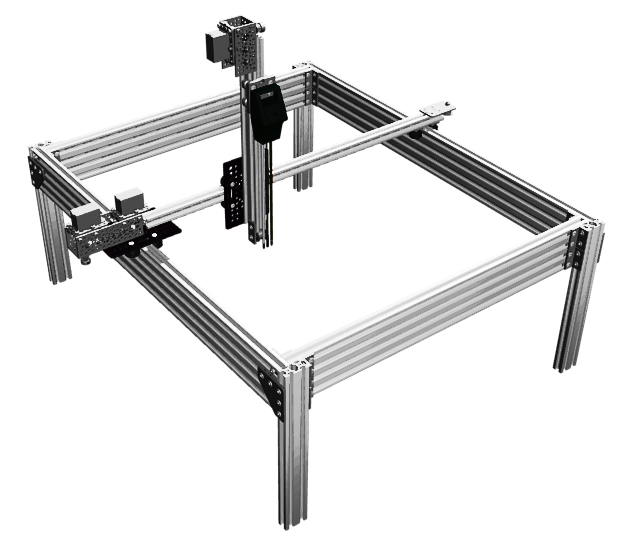
\includegraphics[width=\textwidth]{construct_device_2.png}
    \end{center}
\end{figure}

\section{Μηχανή CNC}

Μηχανή αριθμητικού ελέγχου (Numerical Control -- NC)\index{αριθμητικός
έλεγχος, NC} είναι μία μηχανή η οποία δέχεται κωδικοποιημένες οδηγίες για την
εκτέλεση των επιθυμητών ενεργειών και, κατά βάση, αναφέρεται στον έλεγχο των
εξαρτημάτων της συσκευής παρά σε συγκεκριμένου τύπου μηχανή
\parencites{seames01}{albert11}.

Αρχικά, οι εντολές δίνονταν στη μηχανή μέσω διάτρητων καρτών ή χαρτοταινιών,
ωστόσο, η εξέλιξη των μικροϋπολογιστών επέτρεψε τη χρήση τους για την εκτέλεση
του προγράμματος (Computer Numerical Control - CNC)\index{αριθμητικός
έλεγχος με υπολογιστή, CNC} \parencite{seames01}.

Δεδομένου του ορισμού μία μηχανής CNC, η συσκευή δεν μπορεί να θεωρηθεί ως
τέτοια. Βασικός λόγος είναι ότι η συσκευή αυτοματοποιεί μία διαδικασία δεχόμενη
κάποιες παραμέτρους που ρυθμίζουν ελαφρώς ορισμένες λειτουργίες της χωρίς,
ωστόσο, να απαιτείται η παροχή ενός συνόλου οδηγιών οι οποίες ελέγχουν τα μέρη
της για την πραγματοποίηση της επιθυμητής εργασίας, όπως δηλαδή, απαιτείται από
μηχανές CNC.
Ωστόσο, κρίνεται χρήσιμη η γνωριμία με τέτοια συστήματα καθώς, ακολουθώντας μία
εξελικτική πορεία από το 1952, έχει συσσωρευτεί εμπειρία η οποία μπορεί να φανεί
χρήσιμη για τις ανάγκες της συσκευής.

Ένα από τα ζητήματα που έχουν κληθεί να αντιμετωπίσουν είναι η κίνηση των
εξαρτημάτων τους στο χώρου. Έχουν αναπτυχθεί διάφορες για το σκοπό αυτό οι
οποίες μελετώνται για την ανάδειξη κάποιας κατάλληλης για την υλοποίηση.


\subsection{Διατάξεις CNC}

Η τράπεζα ενός CNC είναι η επιφάνεια πάνω στη οποία εναποτίθεται το προς
επεξεργασία υλικό του συστήματος η οποία είναι δυνατό να κινείται προκειμένου να
εξυπηρετεί κίνηση σε κάποιον άξονα ή να είναι πλήρως σταθερή. Βάσει αυτού του
χαρακτηριστικού, οι διατάξεις CNC διακρίνονται σε κινητής και σταθερής τραπέζης.

Πέραν των διατάξεων που αναφέρονται παρακάτω, υφίστανται κι άλλες που βρίσκουν
εφαρμογή στην
επεξεργασία μεγάλων τρισδιάστατων αντικειμένων, όπως διατάξεις 5 διαστάσεων ή
βιομηχανικά ρομπότ, υποστηρίζοντας περιστροφική κίνηση γύρω από άξονες
επιπροσθέτως της ευθύγραμμης κίνησης σε αυτούς, οι οποίες ξεπερνούν δραματικά
τις απαιτήσεις της υλοποίησης και, συνεπώς, αποκλείονται από αυτήν.

\subsubsection{Κινητή τράπεζα}

\begin{figure}
    \caption{Διατάξεις κινητής τραπέζης.
        \label{fig:construct:cnc_moving-table}}
    \begin{center}
        \begin{subfigure}[b]{0.30\textwidth}
            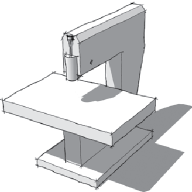
\includegraphics[width=0.95\textwidth]{construct_cnc_xy-table.png}
            \caption{}
        \end{subfigure}
        \begin{subfigure}[b]{0.45\textwidth}
            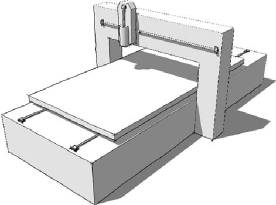
\includegraphics[width=0.9\textwidth]{construct_cnc_moving-table.png}
            \caption{}
        \end{subfigure}
    \end{center}

    (αʹ): \fullcite{albert11:xy-table}

    (βʹ): \fullcite{albert11:moving-table}
\end{figure}

Αναφέρονται δύο διατάξεις που χρησιμοποιούν κινητή τράπεζα. Σε κάθε περίπτωση, η
κίνηση στον κατακόρυφο προς την τράπεζα άξονα, Z, εκτελείται από σταθερό σημείο.
Στην πρώτη διάταξη, η τράπεζα κινείται τόσο στον άξονα X όσο και στον άξονα Y,
με την κίνηση στον άξονα Z να εκτελείται από σταθερή δοκό που εκτείνεται πάνω
από την τράπεζα, στερεωμένη στη βάση μέσω κατακόρυφης στήλης (σχήμα
\ref{fig:construct:cnc_xy-table}α) \parencite[69]{albert11}.
Η τράπεζα αυτής της διάταξης περιορίζεται σε, σχετικά, μικρές διαστάσεις καθώς,
παράλληλα με αυτές, αυξάνει και το μήκος της δοκού και οι απαιτήσεις για τη
στερέωσή της.

Σε εναλλακτική διάταξη, η κίνηση στο επίπεδο X-Y διαμοιράζεται μεταξύ της
τραπέζης και μίας κεφαλής η οποία κινείται στον έναν εκ των δύο αξόνων πάνω σε
γεφύρωμα που διατρέχει όλο το πλάτος της συσκευής (σχήμα
\ref{fig:construct:cnc_xy-table}β) \parencite[70]{albert11}.

Οι διατάξεις κινητής τραπέζης έχουν το μειονέκτημα ότι η κίνηση της τραπέζης
επιβαρύνεται από το υπό παρακολούθηση υλικό θέτοντας περιορισμούς στο μέγιστο
επιτρεπτό βάρος του φορτίου.
Ένα δεύτερο μειονέκτημα είναι ότι η βάση της συσκευής πρέπει να είναι αρκετά
μεγαλύτερη από την τράπεζα μόνο και μόνο για την εξυπηρέτηση της κίνησης με
αποτέλεσμα να δεσμεύεται επιπρόσθετος χώρος χωρίς αυτός να αξιοποιείται
ουσιαστικά για τις ανάγκες της υποβοηθούμενης διαδικασίας.


\subsubsection{Σταθερή τράπεζα}

Σε μία πρώτη διάταξη σταθερής τραπέζης χρησιμοποιείται κινητή στήλη στήριξης
μίας, επίσης, κινητής δοκού, έκαστη κινούμενη σε διαφορετικό άξονα (σχήμα
\ref{fig:construct:cnc_fixed-table}α) \parencite[70]{albert11}. Άμεση πρόκληση
αυτής της διάταξης, η οποία απορρέει από το ότι η δοκός στηρίζεται μόνο σε μία
πλευρά, σχετίζεται με τη σταθερότητα της δοκού ιδίως με την επιμήκυνση της για
την κάλυψη μεγαλύτερης επιφάνειας.

Εναλλακτική διάταξη μοιάζει με τη δεύτερη διάταξη κινούμενης τραπέζης που έχει
αναφερθεί με τη διαφορά ότι αντί για την τράπεζα, κινείται το γεφύρωμα (σχήμα
\ref{fig:construct:cnc_fixed-table}β) \parencite[71]{albert11}.
Ένα ενδεχόμενο μειονέκτημα αυτής της περίπτωσης είναι η ανάγκη για ύπαρξη
εξαρτημάτων κίνησης σε κάθε άκρο του γεφυρώματος.

\begin{figure}
    \caption{Διατάξεις σταθερής τραπέζης.
        \label{fig:construct:cnc_fixed-table}}
    \begin{center}
        \begin{subfigure}[b]{0.40\textwidth}
            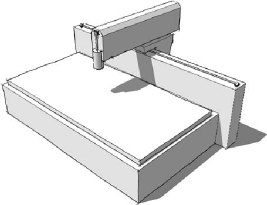
\includegraphics[width=0.95\textwidth]{construct_cnc_cantilevered.png}
            \caption{}
        \end{subfigure}
        \begin{subfigure}[b]{0.40\textwidth}
            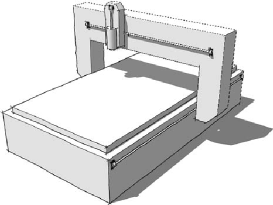
\includegraphics[width=0.9\textwidth]{construct_cnc_moving-gantry.png}
            \caption{}
        \end{subfigure}
    \end{center}

    (αʹ): \fullcite{albert11:cantilevered}

    (βʹ): \fullcite{albert11:moving-gantry}
\end{figure}


\subsection{Υπόδειγμα κατασκευής}

Μεταξύ των δύο κατηγοριών διατάξεων που έχουν αναφερθεί, προτιμώνται διατάξεις
σταθερής τραπέζης κι αυτό επειδή, αφενός, αξιοποιούν καλύτερα το χώρο που τους
αφιερώνεται, αφετέρου επηρεάζουν και επηρεάζονται λιγότερο από τα χαρακτηριστικά
του δοχείου.
Σε σχέση με το δεύτερο, κρίνεται αναπόφευκτη η εξάρτηση των διαστάσεων του
δοχείου από τις διαστάσεις της συσκευής, δεδομένου ότι η συσκευή το πλαισιώνει
και κινείται γύρω από αυτό, ανεξαρτήτως της επιλεγμένης διάταξης. Ωστόσο, η μάζα
του φορτίου, η οποία εξαρτάται από τη μάζα των περιεχόμενων υλικών καθώς και την
απορροφητικότητα τους και την εκάστοτε υγρασία που επικρατεί στο δοχείο, χρήζει
μελέτης μόνο στην περίπτωση των διατάξεων κινητής τραπέζης. Επιλέγοντας
διατάξεις που διατηρούν μονίμως σταθερή την τράπεζα, εξαλείφονται ενδεχόμενοι
περιορισμοί στο μέγιστο επιτρεπτό φορτίο.
%
%Ωστόσο, το μέγιστο επιτρεπτό βάρος του δοχείου, το οποίο επηρεάζεται από τη μάζα
%των υλικών και την απορροφητικότητα τους
%
%Τα όρια, μέγιστα και ελάχιστα, των διαστάσεων του δοχείου υπόκεινται σε
%πρακτικούς περιορισμούς που σχετίζονται, κυρίως, με τη φυσιολογία του πληθυσμού.
%
%Επίσης, θεωρείται καλύτερη πρακτική η δυνατότητα επέκτασης της συσκευής ώστε να
%φιλοξενεί περισσότερη ποσότητα υλικών, χωρίς να απαιτείται αναπροσαρμογή μίας
%τόσο βασικής λειτουργίας της, αυτής της κίνησης.

Επόμενο στοιχείο που μελετάται είναι η αναγκαιότητα ύπαρξης τραπέζης. Δεδομένου
ότι στο δοχείο επικρατούν συνθήκες υψηλής υγρασίας και η κατασκευή αποτελείται
κυρίως από μέταλλο, κρίνεται σκόπιμο τα δύο να είναι πλήρως ανεξάρτητα.
Παράδειγμα αποτελεί η αποστράγγιση, η οποία αν παρέχεται από το δοχείο είναι
προτιμότερο να μην έρχεται σε επαφή με τη συσκευή.
Με αυτόν τον τρόπο, αποφεύγεται η οξείδωση μερών της συσκευής ενώ παράλληλα
επιτρέπεται η ελεύθερη επιλογή, διαμόρφωση και αντικατάσταση του δοχείου χωρίς
να επηρεάζεται η ίδια η συσκευή.
Η ανεξαρτησία του δοχείου σε σχέση με τη συσκευή σε συνδυασμό με το ότι δεν
είναι απαραίτητη η πρόσδεση του για την κίνηση, αποτελούν τους βασικούς λόγους
για την περαιτέρω απάλειψη της τραπέζης.

Σε σχέση με τις δύο προαναφερθείσες διατάξεις σταθερής τραπέζης, επιλέγεται αυτή
του κινητού γεφυρώματος επειδή παρέχει σταθερότητα με περισσότερη ευκολία.


\section{Σύστημα κατασκευής}

Κρίνεται απαραίτητη η εύρεση και αξιοποίηση ενός συστήματος κατασκευής αρχετύπων
που επιταχύνει τη διαδικασία κατασκευής παρέχοντας ευελιξία στην τροποποίηση της
υλοποίησης καθώς αυτή αναπτύσσεται και προκύπτουν νέες απαιτήσεις ή και
προβλήματα, η οποία, ενδεχομένως, παρέχει λύσεις σε συχνές ανάγκες στο πλαίσιο
κατασκευής.

Εντοπίστηκαν αρκετά συστήματα (ουσιαστικά το 80/20 και παραλλαγές αυτού όπως
Misumi, MakerBeam) τα οποία χρησιμοποιούν ράβδους εξωθημένου αλουμινίου ως
δομικά στοιχεία τα οποία συνδυάζονται μεταξύ τους μέσω προσαρτημάτων για την
κατασκευή του σκελετού της κατασκευής.

Η εξώθηση αλουμινίου είναι μία τεχνολογία πλαστικής, δηλαδή μόνιμης,
παραμόρφωσης όπου αλουμίνιο εξωθείται να διέλθει μέσω ενός ανοίγματος
συγκεκριμένου σχήματος για την δημιουργία ράβδων αντίστοιχης διατομής, και τα
προϊόντα της βρίσκουν εφαρμογή σε διάφορους τομείς όπως στην αρχιτεκτονική,
τη βιομηχανία αυτοκινήτων και την παραγωγή μικρών μηχανικών και δομικών
στοιχείων \parencite{saha00}.

Το θετικό αυτής της λύσης είναι ότι χρησιμοποιούνται ξεχωριστά προσαρτήματα για
τη στερέωση των ράβδων και όχι μόνιμη οξυγονοκόλληση επιτρέποντας την ανά πάσα
στιγμή αναδιαμόρφωση των συνδέσεων ενόψει νέων απαιτήσεων ή προβλημάτων και,
λόγω της μορφής τους, επιτρέπουν την ενασχόληση με μεμονωμένα τμήματα με την
περαιτέρω σύνθεσή τους στην τελική κατασκευή.
Για την εξυπηρέτηση ευθύγραμμης κίνησης, οι ράβδοι χρησιμοποιούνται σε συνδυασμό
με τροχοφόρες διατάξεις ή διατάξεις που φέρουν ένσφαιρους τριβείς των ιδίων ή
διαφορετικών συστημάτων.

Επιπροσθέτως αυτών, εντοπίστηκαν συστήματα που αφοσιώνονται εξ ολοκλήρου στη
γραμμική κίνηση, όπως Thomson Linear, Rexroth Bosch Group, NSK Linear.
Μολονότι τα εν λόγω συστήματα, ενδεχομένως, χρησιμοποιούνται κατά κόρον σε
βιομηχανικές εφαρμογές, οι απαιτήσεις αυτής της εφαρμογής είναι αρκετά
διαφορετικές. Ενδιαφέρει περισσότερο η ευελιξία κατά την υλοποίηση (όπως η
δυνατότητα χρήσης οποιασδήποτε δοκού ως οδηγό κίνησης), η ευκολία αναπροσαρμογής
των στοιχείων (για παράδειγμα, χρήση αλουμινίου αντί του πιο σκληρού χάλυβα),
και οι χαμηλές απαιτήσεις συντήρησης, όπως ελάχιστη ή καθόλου ανάγκη για λίπανση
εξαρτημάτων (για παράδεγιμα, για την επιμήκυνση της διάρκειας ζωής τους), και
όλα αυτά, ακόμα και εις βάρους της συνολικής απόδοσης της κατασκευής ή ενός
λιγότερου κομψού αποτελέσματος.

%Επιπλέον, δεδομένων των εγγενώς χαμηλών απαιτήσεων της τρέχουσας εφαρμογής,

Το επιλεγμένο σύστημα διαθέτει όλα τα προαναφερθέντα χαρακτηριστικά. Ένας
επιπρόσθετος λόγος για την επιλογή αυτού έναντι αντίστοιχων συστημάτων είναι
ότι παρέχει μία ποικίλη συλλογή δομικών στοιχείων χωρίς, ωστόσο, να είναι
αχανής, ικανή να καλύψει πληθώρα αναγκών. Επιπλέον, υπερτερεί στο κομμάτι του
αναμενόμενου χρόνου ζωής των τροχών, ενός αναμφισβήτητα σημαντικού δομικού
στοιχείου αυτών των συστημάτων. Τέλος, τα στοιχεία παρέχονται ως ανοικτό υλικό
με ελεύθερη τη λήψη αρχείων για την ενσωμάτωσή τους σε εφαρμογές σχεδίασης 3-Δ.

%Προτιμάται η χρήση τροχοφόρων διατάξεων έναντι ένσφαιρων τριβέων ευθύγραμμης
%κίνησης επειδή οι τριβείς συνήθως απαιτούν λίπανση και περιβάλλον ελεύθερο από
%ρύπους για τη μεγιστοποίηση της απόδοσης και της διάρκειας ζωής τους (REF).

Στη συνέχεια παρουσιάζεται ο τρόπος ενσωμάτωσης δομικών στοιχείων του συστήματος
OpenBuilds για τις ανάγκες της υλοποίησης.


\section{Οδηγοί}

Το βασικότερο δομικό στοιχείο του συστήματος είναι το VSlot, εφεξής οδηγός, το
οποίο
χρησιμοποιείται τόσο για την κατασκευή του σκελετού όσο και για γραμμική κίνηση,
επιτρέποντας οποιοδήποτε τμήμα της κατασκευής να χρησιμοποιηθεί ως φορέας
κινητών φορτίων.

Οι οδηγοί διαθέτουν αυλακώσεις οι οποίες, επικλινείς στο ανώτερο τμήμα,
χρησιμοποιούνται ως διάδρομοι τροχών και ως υποδοχείς ιμάντα, καλωδίων ή άλλων
συνδετικών εξαρτημάτων στο κατώτερο τμήμα.
Στο σχήμα \ref{fig:construct:vslot} παρατίθεται η μορφή των τεσσάρων διαθέσιμων
μεγεθών οδηγών.
Κατασκευάζονται σε μήκος 1 και 1.5m από κράμα αλουμινίου 6063-T5 -- μέταλλο
μαλακό -- το οποίο επιτρέπει την εύκολη αναπροσαρμογή του μήκους τους.

\begin{figure}
    \caption{Τα τέσσερα μεγέθη οδηγών V-Slot.
    \label{fig:construct:vslot}}
    \begin{center}%
    \def\svgwidth{0.8\textwidth}
    \input{img/construct_vslot.pdf_tex}
    \end{center}

    Αρχέτυπο σχέδιο:
\end{figure}


%\subsection{Τροχοί}
\section{Τροχοί}

Συντίθενται από ανεξάρτητα μέρη, με αυτόν τον τρόπο επιτρέποντας την προσαρμογή
τους στις απαιτήσεις κάθε περίπτωσης, την αντικατάσταση κάποιου πιθανού
ελαττωματικού μέρους αντί ολόκληρου του τροχού καθώς και πιθανές μελλοντικές
επεκτάσεις της κατασκευής τους.
Το επίσωτρο των τροχών διαθέτει, σαφώς, συμβατή μορφή με τις αυλακώσεις των
οδηγών και εφάπτεται στο ανώτερο τμήμα των αυλακώσεων δίχως να εισέρχεται πλήρως
μέσα σε αυτές ώστε να αποφεύγονται φθορές στον τροχό κατά την κίνησή του από την
επαφή του με τα τοιχώματα.
%Στην εσωτερική κοιλότητα του επίσωτρου τοποθετείται, εφαρμοστά, ζεύγος ένσφαιρων
%τριβέων για τη μείωση των τριβών μεταξύ του τροχού και του άξονα περιστροφής.
%Στο σχήμα \ref{fig:construct:wheel_exploded} παρατίθενται τα μέρη που συνθέτουν
%έναν υποδειγματικό τροχό· βίδα M5, διαχωριστικό, ένσφαιρος τριβέας, επίσωτρο,
%δακτύλιος, δεύτερος ένσφαιρος τριβέας, αντιπερικόχλιο. Ο λόγος ύπαρξης του
%έκκεντρου διαχωριστικού (eccentric spacer) αιτιολογείται σε επόμενη παράγραφο.
% ως άξονας περιστροφής και για την πρόσδεση του τροχού

Στο σχήμα \ref{fig:construct:wheel_exploded} παρατίθενται τα μέρη που συνθέτουν
έναν υποδειγματικό τροχό, και, συνοπτικά περιγράφονται παρακάτω:
\begin{flushleft}
\begin{description}
    \item[Βίδα M5 (α)] ως άξονας περιστροφής και για την στερέωση του τροχού.
    \item[Διαχωριστικό (β)] για την κάλυψη της απόστασης μέχρι την αυλάκωση.
    \item[Έκκεντρο διαχωριστικό (γ)] ως εναλλακτικό του απλού διαχωριστικού. Η
    χρήση αυτού αντί του απλού διαχωριστικού περιγράφεται σε επόμενη παράγραφο.
    \item[Ένσφαιροι τριβείς (δ)] για την μείωση των τριβών μεταξύ τροχού και
    άξονα περιστροφής.
    \item[Επίσωτρο (ε)] για την επαφή με την αυλάκωση.
    \item[Δακτύλιος (στ)] ενδιάμεσος των τριβέων, για την αποφυγή συμπλοκής
    τους.
    \item[Αντιπερικόχλιο (ζ)] για τη συγκράτηση του τροχού στον άξονα.
\end{description}
\end{flushleft}

\begin{figure}
    \caption{Μέλη που αποτελούν τον τροχό.\label{fig:construct:wheel_exploded}}
    \begin{center}%
    \def\svgwidth{0.8\textwidth}
    \input{img/construct_wheel_exploded.pdf_tex}
    \end{center}
    Αρχέτυπο σχέδιο:
\end{figure}

Οι τροχοί στερεώνονται απευθείας στις αυλακώσεις κάποιου οδηγού δίνοντάς του τη
δυνατότητα κύλισης ή σε ξεχωριστή διάτρητη πλάκα η οποία μπορεί να φιλοξενήσει
και πληθώρα άλλων εξαρτημάτων. Η βασικότερη πλάκα είναι η Universal Gantry
Plate, εφεξής πλάκα γεφυρώματος, το αρχέτυπο της οποίας απεικονίζεται στο σχήμα
\ref{fig:construct:gantry-plate}. Οι περισσότερες κυκλικές οπές της είναι
διαμέτρου 5mm ενώ οι επιμήκεις μπορούν να χρησιμοποιηθούν για την πρόσδεση
ιμάντων.

\begin{figure}
    \caption[Πλάκα γεφυρώματος]{Πλάκα γεφυρώματος (μονάδες σε mm).
    \label{fig:construct:gantry-plate}}
    \begin{center}%
    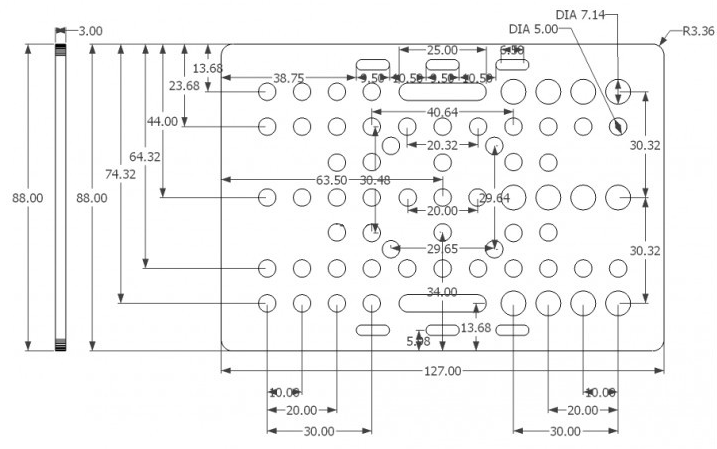
\includegraphics[width=\textwidth]{construct_gantry-plate.png}%
    \end{center}

    \fullcite{carew:gantry-plate-schematic}
\end{figure}

Ορισμένες οπές είναι διαμέτρου 7.14mm και βρίσκονται συγκεντρωμένες στο δεξί
μισό του σχήματος.
Οι συγκεκριμένες χρησιμοποιούνται σε συνδυασμό με έκκεντρα διαχωριστικά έναντι
απλών (σχήμα \ref{fig:construct:wheel_exploded}γ) των οποίων η προεξοχή
εισέρχεται στην οπή. Περιστρέφοντας τους, μεταβάλλεται η απόσταση των
αντίστοιχων τροχών από τον οδηγό έως ότου εφάπτονται ερμητικά με την αυλάκωση
ώστε να αποφεύγονται οι κραδασμοί κατά την κίνηση της πλάκας.
Τοποθετώντας τροχούς σε κατάλληλα ζεύγη οπών 5 και 7.14mm δημιουργείται διάκενο
στο οποίο εισέρχεται οποιοδήποτε από τα τέσσερα μεγέθη οδηγών.


%\section{Γραμμική κίνηση}


\section{Βάση}

\label{sec:construct:base}
Η βάση της συσκευής αποτελείται από πλαίσιο κατασκευασμένο από παραλληλεπίπεδους
οδηγούς, αναρτημένο σε τέσσερις γωνιακούς οδηγούς στήριξης. Η συγκράτηση των
οδηγών επιτυγχάνεται με χρήση γωνιακών προσαρτημάτων, κοχλιών M5 και περικοχλίων
ένθετων στις αυλακώσεις των οδηγών (σχήμα \ref{fig:construct:base}). Όπως
γίνεται αντιληπτό, στοιχεία όπως κοχλίες, περικόχλια, αντιπερικόχλια, δακτύλιοι
\etc{.} είναι απαραίτητα σε κάθε στάδιο της κατασκευής. Ωστόσο, σημειώνεται ότι
αποφεύγεται η τόσο λεπτομερής ανάδειξη των επιμέρους αυτών στοιχείων, εφόσον
κρίνεται ότι στερούνται ουσιαστικού ενδιαφέροντος.

Στον κενό χώρο που σχηματίζεται κάτω από το πλαίσιο, τοποθετείται το δοχείο
παρακολούθησης το οποίο και τον καλύπτει χωρίς, ωστόσο, να εισέρχεται στο
πλαίσιο. Ο χώρος του πλαισίου αφιερώνεται, εξ ολοκλήρου, στην κίνηση των οργάνων
της συσκευής και είναι απαραίτητο να παραμένει ελεύθερος από εμπόδια. Αυτός
είναι και ο λόγος που έχουν επιλεγεί για το πλαίσιο οι τόσο πλατιοί οδηγοί των
8cm· ώστε να καλύπτονται επαρκώς τα κινητά του όργανα καθώς και να παρέχεται ένα
εύληπτο όριο για το ύψος του δοχείου. Περισσότερες λεπτομέρειες σχετικά με τα
κινητά όργανα που προστατεύονται από το πλαίσιο δίνονται στην ενότητα
\nameref{sec:construct:z-axis} (σ.~\pageref{sec:construct:z-axis}).

Το ύψος της βάσης και, συνεπώς, του δοχείου, περιορίζεται από το μέγεθος των
ίδιων των αισθητήριων οργάνων καθώς θα ήταν άσκοπο έως και επιβαρυντικό για την
εξαγωγή έγκυρων μετρήσεων, εάν υπάρχει βάθος στο δοχείο το οποίο παραμένει
απροσπέλαστο από τους αισθητήρες και αδύνατο να καταμετρηθεί.
Δεδομένου ότι οι επιλεγμένοι αισθητήρες υγρασίας και οξύτητας έχουν μήκος
περίπου 21cm, για τη στήριξη του πλαισίου επιλέγονται οδηγοί 30cm, 8cm των
οποίων χρησιμοποιούνται για την προσάρτησή τους στο πλαίσιο (σχήμα
\ref{fig:construct:base}).

Οι άλλες δύο διαστάσεις είναι σχεδόν ανεξάρτητες με τους μοναδικούς περιορισμούς
να τίθενται σχεδόν κατά αποκλειστικότητα από τις δυνατότητες του
μικροεπεξεργαστή καθώς και από πρακτικούς λόγους όπως το μέγεθος της επιφάνειας
προς διαχείριση.
Ωστόσο, επειδή έχει γίνει ήδη αναφορά στο μέγεθος του δοχείου σε σχέση με τη
βάση, σημειώνεται ότι η υπό παρακολούθηση περιοχή είναι ελαφρώς μικρότερη από
τις πραγματικές εσωτερικές διαστάσεις της βάσης εξαιτίας ενός περιθωρίου μερικών
εκατοστών -- μίας περιοχής απροσπέλαστης από τα αισθητήρια όργανα.
Οι λόγοι ύπαρξης του περιθωρίου γίνονται αντιληπτοί στις επόμενες ενότητες.

\begin{figure}
    \caption{Η βάση της συσκευής. \label{fig:construct:base}}
    \begin{center}%
    \def\svgwidth{\textwidth}
    \input{img/construct_base_exploded.pdf_tex}
    \end{center}
\end{figure}


\section{Άξονας Y}

Τροχοφόρος πλάκα τοποθετείται παράλληλα προς το έδαφος με τους τροχούς της στην
κορυφαία αυλάκωση ενός περιμετρικού οδηγού της βάσης. Στο σχήμα
\ref{fig:construct:belt-pulley-y} απεικονίζεται η βασική διάταξη των εξαρτημάτων
σε μία ενδεικτική απλοποιημένη υλοποίηση.
Στην εξωτερική πλευρά της πλάκας (α) βρίσκεται κινητήρας από τον οποίο
εκτείνεται ράβδος (β) που φέρει την κινητήρια τροχαλία (γ) (ο κινητήρας
στερεώνεται πάνω στην πλάκα, ωστόσο, έχει αποκρυφτεί από το συγκεκριμένο σχήμα).
Τραπεζοειδής ιμάντας τεντωμένος κατά μήκος της εξωτερικής αυλάκωσης του οδηγού
και στερεωμένος στα άκρα του, αξιοποιεί τους τροχούς ως ελεύθερες τροχαλίες ώστε
να αυξάνεται το τόξο επαφής με την κινητήρια τροχαλία (γ), παρέχοντας μεγαλύτερη
σταθερότητα κατά την κίνηση.

\begin{figure}
    \caption{Κινητή τροχαλία και ιμάντας. \label{fig:construct:belt-pulley-y}}
Διάταξη τροχαλίας-ιμάντα για την κίνηση στον άξονα Y. Ο κινητήρας έχει
αποκλειστεί από την απεικόνιση. Ωστόσο, νοείται ότι βρίσκεται συζευγμένος με τη
ράβδο (β) στο ελεύθερο άκρο της.
    \begin{center}%
    \def\svgwidth{0.7\textwidth}
    \input{img/construct_belt-pulley-y.pdf_tex}
    \end{center}
\end{figure}


\section{Άξονας X}

Στην ίδια πλάκα, στερεώνεται το ένα άκρο του γεφυρώματος, ένας νέου οδηγού, ο
οποίος ενώνει αυτή με την απέναντι πλευρά της βάσης, πάνω στο οποίο εκτελείται η
κίνηση στον άξονα X.
Ωστόσο, επιλέγεται ελαφρώς διαφορετική προσέγγιση από αυτήν που χρησιμοποιήθηκε
για τον άξονα Y. Βασικό λόγο αποτελεί η τοποθέτηση του κινητήρα και αυτού του
άξονα στην ίδια πλάκα με αυτήν του κινητήρα του άξονα Y, προκειμένου η καλωδίωση
του να εκτείνεται προς ένα κινητό σημείο και όχι, δυνητικά, όλου του πλάτους της
βάσης. Επίσης, με αυτόν τον τρόπο αξιοποιείται μεγαλύτερο μέρος της επιφάνειας
της πλάκας γεφυρώματος.

Στο σχήμα \ref{fig:construct:x-axis-schem} παρουσιάζεται η υλοποίηση του άξονα
X.
Ο κινητήρας X τοποθετείται κοντά στο κέντρο της πλάκας γεφυρώματος (β) με τη
βάση της τροχαλίας (α) παράλληλα προς την πλάκα και ελαφρώς υψηλότερα της ώστε ο
ιμάντας να ευθυγραμμίζεται με αυλάκωση του γεφυρώματος. Η πλάκα φορτίου του
άξονα X τοποθετείται κάθετα ως προς το δάπεδο και ο ιμάντας προσδένεται στις
σχετικές πλαϊνές της οπές. Στην πλευρά της πλάκας πλησιέστερη της τροχαλίας
(στ), ο ιμάντας προσδένεται απευθείας, ενώ στην άλλη, εφόσον διανύσει το μήκος
του γεφυρώματος και αναστραφεί σε ελεύθερη τροχαλία (η) στο άλλο άκρο του.

Στο άκρο της ελεύθερης τροχαλίας, επιλέγεται διαφορετικός τρόπος στερέωσης και
ανύψωσης του οδηγού από τη βάση. Ουσιαστικά, απαλείφεται η πλάκα γεφυρώματος και
χρησιμοποιούνται δύο τροχοί αντί τεσσάρων, οι οποίοι στερεώνονται απευθείας στον
οδηγό. Ο βασικότερος λόγος είναι η αξιοποίηση μεγαλύτερου μήκους του οδηγού,
καθώς μία πλάκα γεφυρώματος, συνολικού μήκους 12.7cm, επιφέρει μεγαλύτερο
περιθώριο (θ) εσωτερικά της βάσης από ότι ένας τροχός. Η επιλογή αυτή
ενδυναμώνεται περαιτέρω από το γεγονός ότι μία πλάκα στο σημείο αυτό θα
χρησιμοποιούταν μόνο για τους τροχούς και την ελεύθερη τροχαλία.

Ωστόσο, παραμένει βασική προϋπόθεση η χρήση κάποιου εξαρτήματος στη θέση της
πλάκας που έχει το ίδιο πάχος, ώστε να διατηρείται οριζόντιος ο οδηγός. Το
μικρότερο εξάρτημα που εντοπίστηκε είναι το πώμα (ζ) το οποίο, τυπικά,
προορίζεται για την κάλυψη των άκρων των οδηγών. Η ορατή έδρα του στο σχήμα, η
οποία διαθέτει μία κοιλότητα, εφάπτεται στον οδηγό. Η άλλη έδρα είναι πλήρως
επίπεδη και σε αυτήν ακουμπά το διαχωριστικό. Επομένως, δεδομένου ότι
χρησιμοποιούνται διαχωριστικά (δ) και επίσωτρα (γ) ίδιου ύψους, ο οδηγός
διατηρείται οριζόντιος.

\begin{figure}
    \caption{Συστατικά μέρη γεφυρώματος. \label{fig:construct:x-axis-schem}}
    \begin{center}%
    \def\svgwidth{\textwidth}
    \input{img/construct_x-axis.pdf_tex}
    \end{center}
\end{figure}

Η ελεύθερη τροχαλία δημιουργείται με επίσωτρο που παρέχει το σύστημα κατασκευής
με τρόπο αντίστοιχο αυτού της σύνθεσης των τροχών. Συνεπώς, ελεύθερες τροχαλίες
μπορούν να τοποθετηθούν απευθείας σε αυλακώσεις οδηγών ή σε πλάκες γεφυρώματος.
Επίσης, παρέχεται και μία διαφορετική μικρότερη πλάκα με λιγότερες οπές ειδικά
για αυτόν το σκοπό (απεικονιζόμενη στο σχήμα \ref{fig:construct:x-axis-schem}η).

Απευθείας προσάρτηση της ελεύθερης τροχαλίας σε αυλάκωση του οδηγού αποκλείεται
σε αυτήν την περίπτωση, καθώς οι διαθέσιμες αυλακώσεις καθιστούν αδύνατη την
άμεση επικοινωνία της με την κινητήρια τροχαλία. Εφόσον έχει ήδη αποκλειστεί η
χρήση πλάκας γεφυρώματος για την αποφυγή άσκοπης σπατάλης χώρου, επιλέγεται η
προσάρτηση της ελεύθερης τροχαλίας στην ειδική πλάκα και, μέσω αυτής, είτε στην
επάνω αυλάκωση του οδηγού (όπως και στο σχήμα \ref{fig:construct:x-axis-schem}),
είτε, εναλλακτικά, στην κάτω αυλάκωση, αντικαθιστώντας το εξωτερικό πώμα.


\section{Άξονας Z}

\label{sec:construct:z-axis}
Τελικά, στην πλάκα φορτίου του άξονα X στερεώνεται το κατώτερο τμήμα οδηγού για
την κίνηση στον άξονα Z, με το μεγαλύτερο τμήμα του να εκτείνεται πάνω από την
πλάκα. Και σε αυτήν την περίπτωση επιλέγεται η χρήση ιμάντα σε συνδυασμό με
κινητήρια και ελεύθερη τροχαλία. Επειδή ενδιαφέρει η μετακίνηση μόνο των
αισθητήρων που προορίζονται για την παρακολούθηση του υλικού, επιλέγεται η πλάκα
Mini~V, η οποία χαρακτηρίζεται από πολύ μικρό μέγεθος, και πάνω σε αυτήν
προσαρτώνται οι αισθητήρες, όπως φαίνεται αριστερά στο σχήμα
\ref{fig:construct:z-axis}. Η εμφανιζόμενη θήκη αποτελεί μέρος των προμηθευμένων
αισθητήρων υγρασίας και οξύτητας η οποία έχει τροποποιηθεί ώστε να στεγάζεται
ένας ακόμα αισθητήρας, αυτός της θερμοκρασίας (γ), και για τη δημιουργία
ορισμένων πρόσθετων οπών για τους κοχλίες και τις γραμμές σήματος.

\begin{figure}
    \caption{Αναπαράσταση οδηγού άξονα Z. \label{fig:construct:z-axis}}
Το μήκος του οδηγού είναι ενδεικτικό και όχι αντιπροσωπευτικό του πραγματικού.
Σημειώνεται ότι στο σχήμα δεξιά εμφανίζεται η διατομή ορισμένων στοιχείων.
    \begin{center}%
    \def\svgwidth{0.5\textwidth}
    \input{img/construct_z-axis.pdf_tex}
    \end{center}
\end{figure}

%belt path
Δεξιά του ίδιου σχήματος εμφανίζεται η διάταξη των στοιχείων που συνθέτουν τον
οδηγό Z. Όπως γίνεται αντιληπτό και από το σχήμα, οι βίδες και τα προσαρτήματα
για τη στερέωση του οδηγού που βρίσκονται χαμηλά στην οπίσθια αυλάκωσή του (α),
αποτρέπουν τη διέλευση του ιμάντα από αυτήν. Για το λόγο αυτό επιλέγεται οδηγός
VSlot~40 ώστε, εναλλακτικά της αυλάκωσης, να αφιερώνεται η ενδιάμεση σήραγγα ως
δίοδος επιστροφής του ιμάντα.

Όπως φαίνεται και στο σχήμα, η ελεύθερη τροχαλία στερεώνεται λίγο διαφορετικά σε
σχέση με τους τρόπους που έχουν προηγουμένως αναφερθεί, αντικαθιστώντας την
ειδική πλάκα με δύο απλά προσαρτήματα. Ο λόγος είναι η αξιοποίηση περισσότερου
μήκους των αισθητήρων, εφόσον τα απλά προσαρτήματα δεσμεύουν λιγότερο χώρο της
αυλάκωσης στην οποία κινείται και η πλάκα Mini~V με αποτέλεσμα, η τελευταία, να
μετακινείται χαμηλότερα στον άξονα Z.

Δεδομένου ότι η πλάκα φορτίου του άξονα X (β) εκτείνεται κάτω από τον οδηγό της,
πρέπει να εξασφαλίζεται ότι και αυτή καθώς και τα υπόλοιπα μέρη, κινούνται χωρίς
να παρεμποδίζονται από τρίτα αντικείμενα. Αυτό αιτιολογεί τη χρήση αρκετά πλατύ
οδηγού για το πλαίσιο της βάσης, όπως αναφέρεται στην ενότητα
\ref{sec:construct:base}.


\section{Τοποθέτηση κινητήρων}

Ενώ το σύστημα κατασκευής OpenBuilds παρέχει πολλά εξαρτήματα για την κάλυψη
πληθώρας αναγκών, έχει, ωστόσο, αποβεί αδύνατος ο εντοπισμός κάποιων που να
διευκολύνουν την τοποθέτηση κινητήρων servo. Αντιθέτως, το σύστημα Actobotics
είναι προσανατολισμένο προς τέτοιους κινητήρες. Μολονότι τα δύο συστήματα
παρουσιάζουν χαμηλή συμβατότητα στα εξαρτήματά τους, μπορούν να συνυπάρξουν, έως
ένα βαθμό.

\begin{figure}
    \caption{Κανάλι Actobotics και διάταξη οπών.
        \label{fig:construct:acto-channel-pattern}}
    \begin{center}
        \begin{subfigure}[b]{0.40\textwidth}
            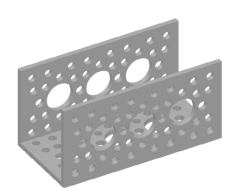
\includegraphics[width=0.95\textwidth]{construct_acto-channel-3in.png}
            \caption{}
        \end{subfigure}
        \begin{subfigure}[b]{0.35\textwidth}
            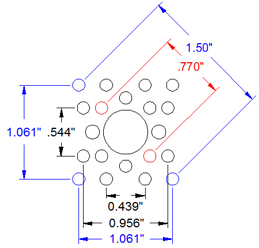
\includegraphics[width=0.9\textwidth]{construct_acto-pattern.png}
            \caption{}
        \end{subfigure}
    \end{center}

    (βʹ): \fullcite{actobotics:channel-pattern}
\end{figure}

Η λύση εντοπίζεται στις κυκλικά διατεταγμένες οπές των καναλιών -- αντίστοιχων
μονάδων των οδηγών VSlot -- οι οποίες απέχουν 0.77in, περίπου 2cm, (σχήμα
\ref{fig:construct:acto-channel-pattern}β), δηλαδή όσο και οι οπές πλακών και
περικοχλίων του OpenBuilds, με αποτέλεσμα να μπορούν να συνδεθούν στα σημεία
αυτά.
Επομένως, επιλέγεται να χρησιμοποιηθούν εξαρτήματα Actobotics για την πλαισίωση
των κινητήρων και, ως βάση, το κανάλι του εν λόγω συστήματος το οποίο στη
συνέχεια προσδένεται σε κάποιο εξάρτημα του συστήματος OpenBuilds. Στην
περίπτωση του κινητήρα Z, το κανάλι προσδένεται απευθείας σε αυλάκωση του 
αντίστοιχου οδηγού ενώ στην περίπτωση των X και Y, πάνω στην πλάκα γεφυρώματος.

Μία κατηγορία εξαρτημάτων του συστήματος Actobotics ιδιαίτερου ενδιαφέροντος
είναι τα στηρίγματα κινητήρα, τα οποία επιτρέπουν πολλές και σύνθετες διατάξεις
τους. Μολονότι παρέχεται στήριγμα που στερεώνεται απευθείας στις γωνιακές οπές
του καναλιού, επιλέγεται στήριγμα που απαιτεί πρόσθετα γωνιακά προσαρτήματα ώστε
ο κινητήρας να εξωθείται ελαφρώς υψηλότερα από το κανάλι προκειμένου να
αξιοποιείται κατά το μέγιστο δυνατό ο χώρος στο εσωτερικό του καναλιού.
Η ανάγκη αυτή προκύπτει για τον κινητήρα του άξονα X όπου η τροχαλία βρίσκεται
στο εσωτερικό του καναλιού. Για περισσότερη ομοιομορφία μεταξύ των κινητήρων,
επιλέγεται η ίδια διάταξη για όλους, παρότι δεν υφίσταται αντίστοιχη επιτακτική
ανάγκη.

\begin{figure}
    \caption{Διάταξη κινητήρων αξόνων X και Y.\label{fig:construct:xy-servo}}
    \begin{center}%
    \def\svgwidth{0.5\textwidth}
%    \input{img/construct_xy-servo.pdf_tex}
    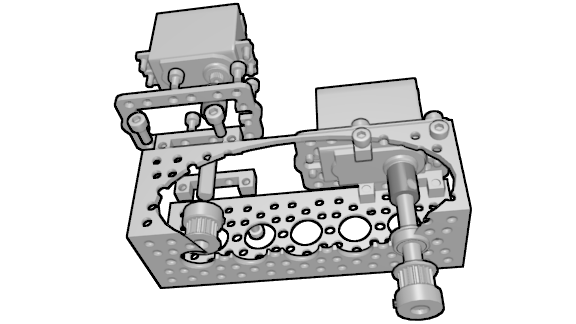
\includegraphics[width=\textwidth]{construct_xy-servo.png}
    \end{center}
\end{figure}
%
%Επιλέγονται γωνιακά προσαρτήματα για την εξώθηση του στηρίγματος του κινητήρα
%ελαφρώς υψηλότερα από το κανάλι ώστε να αξιοποιείται κατά το μέγιστο δυνατό ο
%χώρος στο εσωτερικό του. Η ανάγκη αυτή προκύπτει για τον κινητήρα του άξονα X
%όπου η τροχαλία βρίσκεται στο εσωτερικό του καναλιού. Για περισσότερη
%ομοιομορφία μεταξύ των κινητήρων, επιλέγεται η ίδια διάταξη για όλους, παρότι
%δεν υφίσταται αντίστοιχη επιτακτική ανάγκη.

Στο σχήμα \ref{fig:construct:xy-servo} παρουσιάζεται η διάταξη των στοιχείων για
τους κινητήρες των αξόνων X και Y.
Στην άτρακτο του κινητήρα προσαρτάται σύνδεσμος και, δια μέσω αυτού, το ένα άκρο
ράβδου περιστροφής. Για τους κινητήρες X και Z, η ράβδος είναι αρκετά μακρυά
ώστε να διέρχεται από ένσφαιρο τριβέα τοποθετημένο σε οπή 0.5in του καναλιού. Ο
επιπρόσθετος τριβέας αυξάνει την σταθερότητα της ράβδου, ιδίως όταν στα άκρα της
εφαρμόζεται ακτινικό φορτίο (μέσω του ιμάντα).

Η διατομή της ράβδου είναι σχήματος D και όχι κυκλική ώστε να δημιουργείται μία
επίπεδη επιφάνεια η οποία εξυπηρετεί την ασφαλέστερη πρόσδεση εξαρτημάτων που
διαθέτουν ένθετο κοχλία σύσφιξης. Τόσο ο σύνδεσμος όσο και η κινητήρια τροχαλία
επωφελούνται από αυτήν την ιδιότητα της ράβδου.

\begin{figure}
    \caption{Αναπαράσταση της συσκευής.}
    \begin{center}%
%    \def\svgwidth{0.6\textwidth}
    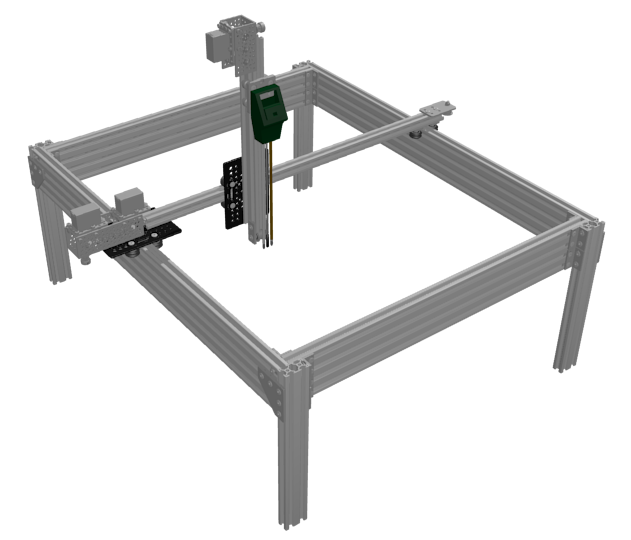
\includegraphics[width=\textwidth]{construct_device.png}
    \end{center}
\end{figure}


%[εικόνα SPLINE SHAFT-COUPLER !BOLT!]

%OPTOCODER

%TMs

%bracket	προσάρτημα στήριξης	Γ.Χαλκιαδάκης,διπλ.αεροναυπηγός μηχανικός

%set screw	κοχλίας πρόσδεσης	ΤΕΕ
%	κοχλίας αξονικής σύσφιξης	Κ.Μπουζάκης,Καθηγητής,Σχολή Μηχανολόγων Μηχανικών

%radial load	ακτινικό φορτίου	JAR 23, Greek CAA;
%		ΒΑΣ.ΦΙΛΟΠΟΥΛΟΣ,Χημικός-Μηχανικός

%punched tape	διάτρητη χαρτοταινία	ΕΠΥ

%machining	μηχανουργική κατεργασία	ΤΕΕ

%structural system	δομικό σύστημα	Dec. 96/582/EC OJ L 254/96 p.62

%plastic deformation	πλαστική παραμόρφωση
%		ΕΛΕΤΟ/Ειδική Ομάδα Ορολογίας Μεταλλουργίας-Μεταλλογνωσίας, Έγκριση ΓΕΣΥ

%cantilevered	πρόβολος δοκός	Κ.Μπουζάκης, καθηγ., σχολή Μηχανολόγων Μηχανικών Α.Π.Θ.

%moving table	κινούμενη τράπεζα	ΙCG-ΕΛΛΗΝΙΚΟΣ ΥΑΛΟΥΡΓΙΚΟΣ ΣΥΝΔΕΣΜΟΣ

%idler pulley	ελεύθερη τροχαλία // τροχαλία έντασης

%pulley	κινητήρια τροχαλία

%τροχαλία με αυλακωτή στεφάνη

\chapter{Κωδικοποιητής κίνησης}
\label{ch:encoder}

Προκειμένου να παρέχεται στο μικροελεγκτή μία ένδειξη για την πορεία της κίνησης
του κάθε κινητήρα, κρίνεται σκόπιμη η ύπαρξη μίας μορφής ανατραφοδότησης· ενός
αισθητήρα που παρακολουθεί κάποιο φυσικό φαινόμενο που σχετίζεται με την κίνηση
του κινητήρα (βλ. σχήμα \ref{fig:encoder:lvl-0}).

\begin{figure}
    \caption{Επίδραση και ανάδραση μικροελεγκτή και κινητήρα.
    \label{fig:encoder:lvl-0}}
    \begin{center}
    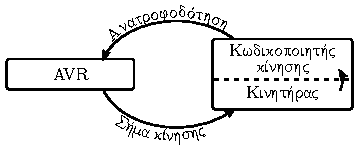
\includegraphics{encoder_lvl-0}
    \end{center}
\end{figure}

Παρότι υπάρχουν διάφορα φαινόμενα που μπορούν να χρησιμοποιηθούν για αυτόν το
σκοπό (όπως μαγνητισμός, ηλεκτρική αντίσταση σε μορφή ποτενσιόμετρου),
επιλέγεται η χρήση των, πλέον ίσως όχι και τόσο διαδεδομένων, υπερύθρων ακτίνων.
Το επιδιωκόμενο αποτέλεσμα παρουσιάζεται στο σχήμα \ref{fig:encoder:lvl-1}.

Όπως φαίνεται στο σχήμα, ο αισθητήρας αποτελείται από έναν πομπό και ένα δέκτη
υπερύθρων ακτίνων (φωτοδίοδος και φωτοτρανζίστορ, αντίστοιχα).
Η άτρακτος είναι ο άξονας περιστροφής του κινητήρα. Πάνω σε αυτόν προσκολλάται
μία ειδικά σχεδιασμένη ταινία, η οποία καθώς περιστρέφεται ως αποτέλεσμα
περιστροφής της ατράκτου, επηρεάζει την ένταση των εκπεμπόμενων ακτίνων του
πομπού που καταφθάνουν στο δέκτη, η οποία, με τη σειρά της, επηρεάζει την ένταση
της εξόδου του. Με αυτόν τον τρόπο επιτυγχάνεται η μετατροπή την στροφικής
κίνησης σε ηλεκτρικούς παλμούς οι οποίοι επιστρέφονται, ιδανικά, ως τετραγωνικοί
παλμοί.

\begin{figure}
    \caption{Σχηματική απεικόνιση κωδικοποιητή υλοποίησης.
    \label{fig:encoder:lvl-1}}
    \begin{center}
    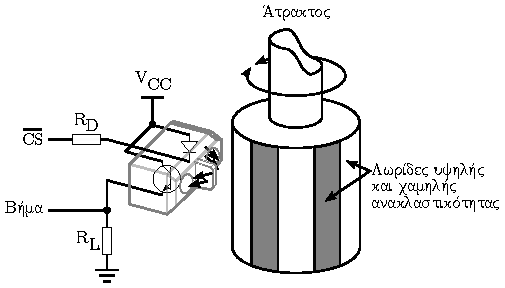
\includegraphics{encoder_lvl-1}
    \end{center}
\end{figure}

Ο αυτοσχέδιος κωδικοποιητής της υλοποίησης πρόκειται για έναν προσαυξητικό
κωδικοποιητή, δηλαδή του οποίου η έξοδος πληροφορεί για την πραγματοποίηση ενός
μικρού βήματος από μία λωρίδα στην επόμενη.
Σε σχέση με τους απόλυτους κωδικοποιητές που πληροφορούν τη συγκεκριμένη θέση
(πιθανώς, σε μοίρες) στην οποία βρίσκεται η άτρακτος, έχει το πλεονέκτημα ότι
είναι πολύ πιο απλός στην υλοποίηση και τη διασύνδεση με το μικροελεγκτή, καθώς
απαιτεί μόνο έναν αισθητήρα και, συνεπώς, μία γραμμή σύνδεσης για κάθε κινητήρα.
Περισσότερα αναφέρονται στην ενότητα \nameref{subsec:encoder:output} (σ.~%
\pageref{subsec:encoder:output}).

Ωστόσο, σε αντίθεση με τη συνήθη μορφή, η υλοποίηση χρησιμοποιεί μία ταινία που
εφάπτεται της ατράκτου αντί δίσκου. Η επιλογή αυτή γίνεται καθαρά για
διευκόλυνση της τοποθέτησης των εξαρτημάτων, παρά την ενδεχόμενη μείωση της
ακρίβειας του κωδικοποιητή.

Η επιλογή του υλικού της ταινίας, το πλάτος των λωρίδων της, η απόσταση και η
διάταξη (κάθετα ή παράλληλα) του αισθητήρα σε σχέση με αυτές καθώς και η γωνιακή
ταχύτητα της ατράκτου επηρεάζουν την ικανότητα αναγνώρισης των μεταβολών από τη
μία λωρίδα στην επόμενη (βλ. \nameref{subsec:reflex:coupling-factor} σ.~%
\pageref{subsec:reflex:coupling-factor}).
Επιπρόσθετα στοιχεία που επηρεάζουν την ακρίβεια του αισθητήρα και, για την
ακρίβεια, την πιθανότητα εσφαλμένης εξόδου από το δέκτη (φωτοτρανζίστορ) είναι
το αναφερόμενο ως ρεύμα ηρεμίας (\te{dark current}) και παρεμβολές από
περιβάλλουσες φωτεινές πηγές, καθώς και η θερμοκρασία εν γένει. Αυτές οι,
δευτερευούσης σημασίας, παράμετροι αναφέρονται στη σελίδα
\pageref{subsec:reflex:other-parameters}.

Στην ενότητα \nameref{subsec:reflex:calculations} (σ.~%
\pageref{subsec:reflex:calculations}) γίνεται μία προσπάθεια εκτίμησης των
ιδιοτήτων των στοιχείων που απαρτίζουν κάθε κωδικοποιητή ώστε να παραχθεί το
επιθυμητό αποτέλεσμα.
Μέρος αυτών των υπολογισμών αφιερώνεται στο προσδιορισμό της αντίστασης των
αντιστατών R\tsub{D} και R\tsub{L} του σχήματος, εκ των οποίων ο πρώτος ελέγχει
την ένταση που διαρρέει τη φωτοδίοδο, ενώ ο δεύτερος, χρησιμεύει για την
παραγωγή δύο διακριτών τιμών (λογικό 0 και 1) ως έξοδο του κωδικοποιητή.


\section{Οπτικοί κωδικοποιητές}
\label{sec:encoder:optical}

Σύμφωνα με έκδοση της \textcite[12]{drc76}, οπτικοί κωδικοποιητές περιστροφικής
κίνησης, παραδοσιακά, κατασκευάζονται με την προσάρτηση ενός περιφερειακά
διάτρητου δίσκου στον άξονα κίνησης εκατέρωθεν του οποίου διατάσσεται αντικριστό
ζεύγος πομπού και δέκτη υπέρυθρων ακτίνων. Καθώς ο δίσκος περιστρέφεται ως
αποτέλεσμα κίνησης του άξονα, η ύπαρξη ή έλλειψη οπής επαναφέρει ή αποκόπτει την
επικοινωνία μεταξύ πομπού-δέκτη προκαλώντας εναλλαγές στην έξοδο του δέκτη
\parencite[12]{drc76}.

\begin{figure}
    \caption{Προσαυξητικός οπτικός κωδικοποιητής με χρήση φωτοδιακόπτη.
    \label{fig:encoder:incremental}}
    \begin{center}
    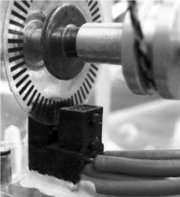
\includegraphics{encoder_incremental}
    \end{center}
    \fullcite{tycho:incremental}
\end{figure}


\subsection{Αναγνώριση θέσης}
\label{subsec:encoder:output}

\subsubsection{Προσαυξητικοί}

Στην απλούστερη υλοποίηση, ο αισθητήρας αναγνωρίζει τη μετάβαση από τη μία θέση
στην επόμενη ενώ είναι αδύνατο να αναχθεί από το σήμα και μόνον, είτε η φορά
περιστροφής είτε η τρέχουσα γωνιακή μετατόπιση του άξονα· ο ελεγκτής είναι
υπεύθυνος για την εξαγωγή αυτών των συμπερασμάτων \parencites[5--6]{lynch02}
[13]{drc76}. Στην περίπτωση αυτή, ο κωδικοποιητής αποκαλείται
προσαυξητικός\index{προσαυξητικός κωδικοποιητής} (incremental)
\parencite[5]{lynch02}. Ένα παράδειγμα προσαυξητικού κωδικοποιητή περιστροφικής
κίνησης παρουσιάζεται στην εικόνα \ref{fig:encoder:incremental}.


\subsubsection{Απόλυτης θέσης}

Ωστόσο, είναι δυνατό να κατασκευαστεί απόλυτος (absolute)
κωδικοποιητής\index{κωδικοποιητής απόλυτης μετατόπισης} μετατόπισης, κάνοντας
χρήση πολλαπλών ζευγών πομπού-δέκτη και ενός δίσκου υποδιαιρεμένου σε διακριτές
θέσεις που αποτελούνται από μοναδικό συνδυασμό οπών \parencites[6]{lynch02}. Ο
κάθε αισθητήρας παράγει έξοδο ανεξάρτητη από τους υπολοίπους βάσει των οπών που
του αντιστοιχούν, ενώ η συνδυαστική έξοδος όλων των αισθητήρων περιγράφει τον
τρέχοντα συνδυασμό οπών και συνεπώς τη γωνιακή μετατόπιση του δίσκου
\parencites[6]{lynch02}.


\subsection{Διάταξη στοιχείων}
\label{subsec:encoder:layout}

Για τη σύνθεση ενός κωδικοποιητή που κάνει χρήση οπτικών αισθητήρων,
χρησιμοποιούνται ζεύγη πομπού και δέκτη υπέρυθρων ακτίνων. Το κάθε ζεύγος μπορεί
να αποτελείται από ανεξάρτητα, μεταξύ τους, στοιχεία ή να βρίσκονται
ενσωματωμένα σε ειδική θήκη που διευκολύνει την τοποθέτησή τους (όπως στην
περίπτωση της εικόνας \ref{fig:encoder:incremental}).


\subsubsection{Φωτοδιακόπτες}

Υπάρχουν διατάξεις που τοποθετούν αντικριστά το ζεύγος πομπού και δέκτη
σχηματίζοντας έναν κενό χώρο μεταξύ τους στον οποίο μπορεί να εισέρχεται
εξωτερικό αντικείμενο, διακόπτοντας την επικοινωνία τους. Τέτοιοι αισθητήρες
αναφέρονται ως φωτοδιακόπτες\index{φωτοδιακόπτης}
(photointerrupter) \parencite[3]{lynch02} και αποτελούν τη διάταξη που
έχει παρουσιαστεί μέχρι τώρα.


\subsubsection{Ανακλαστικοί}

Σε εναλλακτική διάταξη, πομπός και δέκτης είναι μεταξύ τους παρακείμενοι με την
επικοινωνία τους να είναι δυνατή μόνο εφόσον οι εκπεμπόμενες ακτίνες ανακλαστούν
σε εξωτερική επιφάνεια (σχήμα \ref{fig:reflex:tct5000}).
Τέτοιοι αισθητήρες αναφέρονται ως ανακλαστικοί \index{ανακλαστικός αισθητήρας}
(reflective) \parencite[3]{lynch02}.
Η έξοδος του δέκτη επηρεάζεται άμεσα από την ένταση των προσπίπτουσων ακτίνων η
οποία, με τη σειρά της, εξαρτάται από τις ανακλαστικές ιδιότητες και την
απόσταση της εξωτερικής επιφάνειας \parencite{vishay06}.

Για την κατασκευή
οπτικού κωδικοποιητή κάνοντας χρήση αισθητήρα τέτοιας διάταξης, ο προσαρτημένος
στον άξονα περιστροφής δίσκος είναι χωρισμένος σε τμήματα διαφορετικού και
εναλλασσόμενου συντελεστή ανάκλασης ώστε με την περιστροφή του να επηρεάζεται η
ένταση των προσπίπτουσων ακτίνων στον κάθετο ως προς το δίσκο αισθητήρα, και,
συνεπώς, η έξοδός του \parencite[11]{vishay02}.


\section{Ανακλαστικός αισθητήρας TCRT5000}

\begin{figure}
    \caption{Ο ανακλαστικός οπτικός αισθητήρας TCRT5000.
    \label{fig:reflex:tcrt5000}}
    \begin{center}
    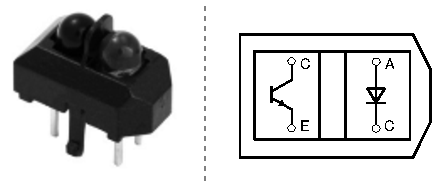
\includegraphics{reflex_tcrt5000}
    \end{center}
    \fullcite{vishay09:tcrt5000}
\end{figure}

Η ενότητα ασχολείται με τις διάφορες παραμέτρους που επηρεάζουν την απόδοση ενός
ανακλαστικού αισθητήρα προκειμένου να προσδιοριστούν οι απαιτήσεις για τη
συνδεσμολογία του με το μικροελεγκτή και την τοποθέτησή του σε σχέση με τους
κινητήρες με γνώμονα την κάλυψη των αναγκών για την παρακολούθηση της κίνησης
των τελευταίων.

Στην περίπτωση του συγκεκριμένου αισθητήρα, TCRT5000, ο δέκτης πρόκειται για ένα
φωτοτραζίστορ· ένα φωτοευαίσθητο ημιαγωγό όπου η ένταση διέλευσης ρεύματος
μεταξύ συλλέκτη (\te{collector}) και εκπομπού (\te{emitter}) ελέγχεται από την
ένταση των προσπίπτουσων ακτίνων, ενώ ο πομπός, μία φωτοδίοδος· ένα ημιαγωγό που
προκαλεί την παραγωγή φωτός (στην προκειμένη υπέρυθρου) όταν διαρρέεται από
ρεύμα. Όπως φαίνεται και στο σχήμα \ref{fig:reflex:tcrt5000}, τα δύο στοιχεία
(φωτοδίοδος και φωτοτρανζίστορ) είναι απομονωμένα μεταξύ τους από ένα ενδιάμεσο
τοίχωμα. Η επικοινωνία τους καθίσταται δυνατή μόνο εφόσον τα πλησιάσει εξωτερικό
αντικείμενο.


\subsection{Συντελεστής σύζευξης}
\label{subsec:reflex:coupling-factor}

Σύμφωνα με τη \textcite{vishay02}, στους ανακλαστικούς αισθητήρες που κάνουν
χρήση φωτοτρανζίστορ, ο λόγος της έντασης ρεύματος του συλλέκτη προς το ρεύμα
ορθής φοράς, $\frac{I_{C}}{I_{F}}$, αναφέρεται ως συντελεστής σύζευξης
\index{συντελεστής σύζευξης} (coupling factor), $k$, και περιγράφει το
βαθμό οπτικής σύνδεσης μεταξύ πομπού και δέκτη.
Ο προσδιορισμός του γίνεται για ορισμένη ανακλαστική επιφάνεια και απόσταση από
αυτήν και επηρεάζεται από την ένταση ρεύματος του πομπού, τη θερμοκρασία και τη
συχνότητα εναλλαγής μεταξύ επιφανειών διαφορετικών συντελεστών ανάκλασης
\parencite{vishay02}.


\subsubsection{Ανακλαστική επιφάνεια}

Ο πίνακας \ref{tab:reflex:materials}, ο οποίος αποτελεί απόσπασμα μετρήσεων της
\textcite{vishay06},
παρουσιάζει το ποσοστό της έντασης ρεύματος που σημειώνεται στο συλλέκτη για
διάφορα ανακλαστικά υλικά σε σχέση με τη χρήση της λευκής όψης κάρτας Kodak
neutral (No\@.Q-13).
Για τις ανάγκες της υλοποίησης, η επιφάνεια κωδικοποίησης είναι αρκετό να
αποτελείται από διαδοχικά τμήματα που παρουσιάζουν μεγάλη απόκλιση στους
συντελεστές ανάκλασης, ώστε να μην παρατηρείται επικάλυψη στο εύρος έντασης
ρεύματος του συλλέκτη για καθένα και, συνεπώς, να αυξάνεται η δυνατότητα
διάκρισή τους. Μία δεύτερη απαίτηση είναι η διαθεσιμότητα και η ευχρηστία των
αντίστοιχων υλικών ώστε να είναι άμεση η ενδεχόμενη αντικατάσταση ή τροποποίηση
της επιφάνειας κωδικοποίησης.

\begin{table}
\caption{Σχετική απόδοση διάφορων ανακλαστικών υλικών.
\label{tab:reflex:materials}}

Σε όλες τις μετρήσεις, το ρεύμα
ορθής φοράς, $I_{F}$, ήταν σταθερό στα 20mA, ο αισθητήρας τοποθετημένος κάθετα
ως προς την ανακλαστική επιφάνεια σε απόσταση όπου ο συλλέκτης αποδίδει τη
μέγιστη έξοδο για υπέρυθρες των 950nm \textcite{vishay06}.\\~

\begin{tabu} to \linewidth{X X[-1,R] X[-1] X X[-1,R]}
\multicolumn2{l}{\bfseries Kodak neutral card}    & &
\multicolumn2{l}{\bfseries Black on white typewritting paper} \\
\cline{1-2}\cline{4-5}

White side (reference medium)           &   100\%   & &
Drawing ink (Higgins, Pelikan)          &   4--6\%  \\

Gray side                               &   20\%    & &
Foil ink (Rotring)                      &   50\%    \\

\multicolumn2{l}{\bfseries Paper}                   & &
Fiber-tip pen (Edding 400)              &   10\%    \\
\cline{1-2}

Typewriting paper                       &   94\%    & &
Fiber-tip pen, black (Stabillo)         &   76\%    \\

Drawing card, white (Schoeller)         &   100\%   & &
Photocopy                               &   7\%    \\

Card, light gray                        &   67\%    & &
\multicolumn2{l}{\bfseries Plotter pen}             \\
\cline{4-5}

Envelope (beige)                        &   100\%   & &
HP fiber-tip pen (0.3mm)               &   84\%     \\

Packing card (light brown)              &   84\%    & &
Black 24 needle printer                 &   28\%    \\

Newspaper paper                         &   97\%    & &
Ink (Pelikan)                           &   100\%   \\

Pergament paper                         &   30--42\% & &
Pencil, HB                              &   26\%    \\
\end{tabu}

\floatfoot{\fullcite[2]{vishay06:materials}}
\end{table}

Με αυτά τα κριτήρια, επιλέγεται το απλό τυπογραφικό χαρτί ως επιφάνεια υψηλού
συντελεστή ανάκλασης (94\%) με την επικάλυψη του με φωτοτυπικό μελάνι ως
επιφάνεια χαμηλού συντελεστή (7\%).

Για περαιτέρω απλούστευση της υλοποίησης, επιλέγεται η αντικατάσταση του δίσκου
κωδικοποίησης με ταινία η οποία καλύπτει την περιφέρεια του άξονα περιστροφής
στο σημείο όπου είναι τοποθετημένος ο αισθητήρας.

%Αναφορά σε πιθανές επιπτώσεις


\subsubsection{Λειτουργική απόσταση}

Η απόσταση του αισθητήρα από την ανακλαστική επιφάνεια επηρεάζει άμεσα το
ποσοστό των προσπίπτουσων ακτίνων στο δέκτη που είναι υπεύθυνες για τη διέγερση
του φωτοτρανζίστορ. Η απόσταση αυτή αποκαλείται λειτουργική απόσταση
\index{λειτουργική απόσταση} (operating distance), $d$, και, για μία
τυπική υλοποίηση, απεικονίζεται στο σχήμα \ref{fig:reflex:working-diagram}(αʹ)
\parencite{vishay02}.

Όπως είναι αναμενόμενο, καθώς η λειτουργική απόσταση μεταβάλλεται, η ένταση
ρεύματος του συλλέκτη αυξομειώνεται. Σύμφωνα με τη τον οδηγό της
\textcite{vishay06}, η σχέση αυτή απεικονίζεται στο λειτουργικό διάγραμμα
\index{λειτουργικό διάγραμμα} (operating diagram) στο εγχειρίδιο χρήσης
κάθε αισθητήρα.

Το σχήμα \ref{fig:reflex:working-diagram}(βʹ) αποτελεί το λειτουργικό διάγραμμα
του επιλεγμένου αισθητήρα, TCRT5000, όπου παρουσιάζεται η ένταση ρεύματος του
συλλέκτη, $I_{C}$, σε σχέση με τη μέγιστη δυνατή, $I_{Cmax}$, καθώς μεταβάλλεται
η λειτουργική απόσταση.
Επίσης, παρατηρείται ότι η μέγιστη ένταση του συλλέκτη, $I_{C} = I_{Cmax}$,
σημειώνεται για μία λειτουργική απόσταση $d = 2.5$cm.

\begin{figure}
    \caption{Λειτουργική απόσταση και λειτουργικό διάγραμμα.
        \label{fig:reflex:working-diagram}}
    \begin{center}
        \begin{subfigure}[b]{0.45\textwidth}
            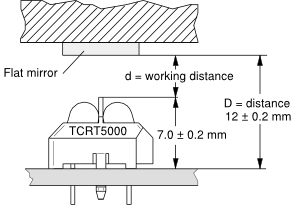
\includegraphics[width=0.95\textwidth]{reflex_test-circuit.png}
            \caption{}
        \end{subfigure}
        \begin{subfigure}[b]{0.45\textwidth}
            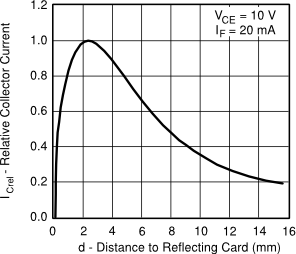
\includegraphics[width=0.9\textwidth]{reflex_working-distance.png}
            \caption{}
        \end{subfigure}
    \end{center}

    (αʹ): \fullcite[3]{vishay09:test-circuit}

    (βʹ): \fullcite[4]{vishay09:working-distance}
\end{figure}

Για τις ανάγκες της υλοποίησης, επιλέγεται λειτουργική απόσταση 2.5cm έτσι ώστε
ο συντελεστής σύζευξης να ευνοείται όσο το δυνατόν περισσότερο.


\subsubsection{Διάστημα εναλλαγής}

Για τις ανάγκες της υλοποίησης, ο άξονας περιστροφής επικαλύπτεται, στο ύψος του
αισθητήρα, από διαδοχικά τμήματα υψηλότερου και χαμηλότερου συντελεστή
ανάκλασης. Καθώς ο άξονας περιστρέφεται, η ένταση ρεύματος του συλλέκτη
μεταβάλλεται από τη μέγιστη μέχρι την ελάχιστη δυνατή και αντίστροφα.
Ωστόσο, σύμφωνα με το εγχειρίδιο της \textcite{vishay06}, εάν το πάχος των
τμημάτων είναι πολύ μικρό, ενδέχεται οι εναλλαγές να μην εκδηλώνονται αισθητά
στην ένταση ρεύματος του συλλέκτη.

Στο σχήμα \ref{fig:reflex:switching-distance} παρουσιάζεται η ένταση ρεύματος
του συλλέκτη για δύο διαδοχικά τμήματα.
Το σημείο εναλλαγής από τον ένα συντελεστή ανάκλασης στον επόμενο σημειώνεται
με το $Xo$ ενώ με $I_{c1}$ και $I_{c2}$, η μέγιστη ένταση ρεύματος του
συλλέκτη όταν η κοινή επιφάνεια $g$ των οπτικών πεδίων πομπού και δέκτη
καλύπτεται πλήρως από τμήμα του αντίστοιχου συντελεστή.
Προκύπτει ότι, ενώ η μετάβαση από τον ένα συντελεστή στον επόμενο συμβαίνει
ακαριαία, η ένταση ρεύματος του συλλέκτη $I_C$ έχει αρχίσει να μειώνεται σε
προγενέστερη μετατόπιση, όταν ένα πρώτο τμήμα των αρχικά διαθέσιμων ακτίνων
αποκόπηκε από το δέκτη, και συνεχίζει να μειώνεται σταδιακά έως ότου το τμήμα με
το νέο συντελεστή έχει καλύψει πλήρως την περιοχή $g$.

\begin{figure}
    \caption{Σχέση μεταβολής ρεύματος $I_C$ και συντελεστή ανάκλασης.
        \label{fig:reflex:switching-distance}}
    \begin{center}
        \begin{subfigure}{0.45\linewidth}
            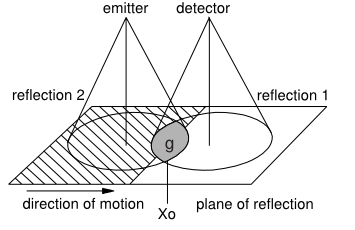
\includegraphics{reflex_switching-distance_a.png}
        \end{subfigure}
        \begin{subfigure}{0.45\linewidth}
            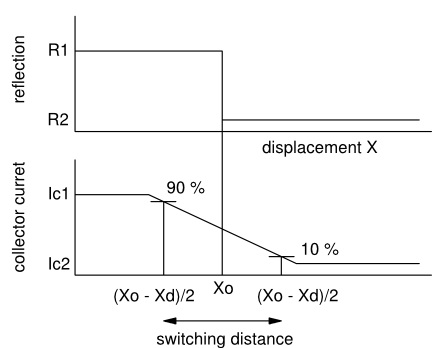
\includegraphics{reflex_switching-distance_b.png}
        \end{subfigure}
    \end{center}
    \fullcite[3]{vishay06:switching-distance}
\end{figure}

Επίσης, συμπεραίνεται ότι, καθώς το πάχος των τμημάτων μειώνεται ώστε η περιοχή
$g$ να είναι αδύνατο να καλυφθεί εξ ολοκλήρου από ένα μόνο τμήμα, η μέγιστη και
ελάχιστη τιμή έντασης ρεύματος που είναι δυνατό να σημειωθούν αρχίζουν να
συγκλίνουν, εφόσον, πλέον, σε κάθε μετατόπιση καταφθάνουν στο δέκτη ακτίνες από
όλο και περισσότερα τμήματα.

Το ελάχιστο πάχος τμημάτων καθορίζεται από το διάστημα εναλλαγής\index{διάστημα%
εναλλαγής} (switching distance),
$X_d$, το οποίο ορίζεται ως το διάστημα μεταξύ δύο διαδοχικών τμημάτων
διαφορετικών συντελεστών ανάκλασης στο οποίο παρατηρείται το 90\% $I_{C_1}$ έως
το 10\% $I_{C2}$ \parencite{vishay06}. Η τιμή του διαστήματος εναλλαγής
εξαρτάται, από την κατασκευή του αισθητήρα καθώς και τη λειτουργική απόσταση,
ενώ όσο πιο μικρή απόσταση εναλλαγής υποστηρίζει κάποιος αισθητήρας, τόσο
υψηλότερη η διακριτική ικανότητά (resolution) του
\parencites{vishay02}{vishay06}. Για τον αισθητήρα TCRT5000, το διάστημα
εναλλαγής ανέρχεται στα 1.9mm \parencite{vishay02}.

Στο σχήμα \ref{fig:reflex:d_switching-distance} παρουσιάζεται πώς η λειτουργική
απόσταση του αισθητήρα επηρεάζει το διάστημα εναλλαγής του. Οι εμφανιζόμενες
καμπύλες αποτελούν ένα κατώτατο όριο και αντιστοιχούν σε δύο διαφορετικούς
τρόπους τοποθέτησης του αισθητήρα σε σχέση με την ανακλαστική επιφάνεια.
Στη θέση~1, ο νοητός άξονας που ορίζεται από πομπό και δέκτη του αισθητήρα είναι
κάθετος ως προς τα εναλλασσόμενα τμήματα, ενώ στη θέση~2, παράλληλος.
Παρατηρείται ότι η θέση~1 υπερτερεί της θέσης~2 καθώς για την ίδια λειτουργική
απόσταση επιτυγχάνεται υψηλότερη διακριτική ικανότητα και, συνεπώς, προσφέρεται
υψηλότερο ελάχιστο διάστημα εναλλαγής. Δεδομένου ότι οι συνθήκες (ανάγκες και
περιορισμοί) το επιτρέπουν, επιλέγεται η θέση~1 για την υλοποίηση.

\begin{figure}
    \caption{Σχέση Λειτουργικής απόστασης και Διαστήματος εναλλαγής.
    \label{fig:reflex:d_switching-distance}}
    \begin{center}%
    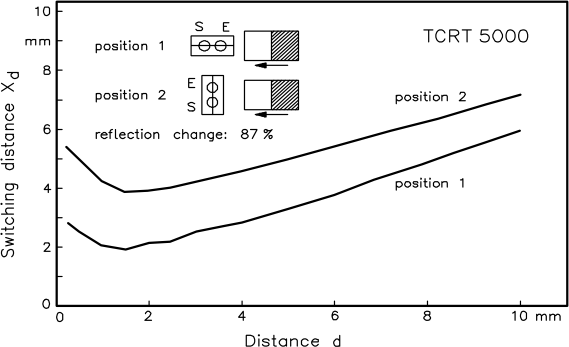
\includegraphics[width=0.7\textwidth]{reflex_d_switching-distance.png}%
    \end{center}

    \fullcite[8]{vishay02:d_switching-distance}
\end{figure}


\subsubsection{Συχνότητα αποκοπής}

Το φωτοτρανζίστορ---το πιο αργό στοιχείο του αισθητήρα---απαιτεί κάποιο χρόνο
για να ανταποκριθεί στις απότομες εναλλαγές έντασης των προσπίπτουσων ακτίνων
\parencite{vishay06}. Ως αποτέλεσμα, εάν οι νέες εναλλαγές προκύπτουν προτού η
έξοδος του να έχει κατασταλάξει για μία προηγούμενη εναλλαγή, τότε η αναγνώρισή
τους καθίσταται μάλλον αβέβαιη. Άμεση απόρροια αυτού, δηλαδή του χρόνου
απόκρισης του φωτοτρανζίστορ, είναι η ανάγκη προσδιορισμού μίας μέγιστης
επιτρεπόμενης συχνότητας εναλλαγής των τμημάτων διαφορετικού συντελεστή
ανάκλασης ώστε να μην επηρεάζεται δραματικά ο συντελεστής σύζευξης. Η συχνότητα
αυτή αναφέρεται ως συχνότητα αποκοπής \index{συχνότητα αποκοπής}
(cut-off frequency) και είναι η συχνότητα στην οποία παρατηρείται μείωση
περίπου 30\% του συντελεστή σύζευξης \parencite{vishay02}.

Το σχήμα \ref{fig:reflex:cutoff-frequency} παρουσιάζει πώς επηρεάζουν η τάση και
η αντίσταση φόρτου, $R_L$, του φωτοτρανζίστορ τη συχνότητα αποκοπής του
αισθητήρα.
Θα μπορούσε να χρησιμοποιηθεί χαμηλή τιμή αντίστασης φόρτου, ώστε να
μειωθεί ο χρόνος απόκρισης και, ως επέκταση, να διευρυνθεί το όριο της
συχνότητας αποκοπής. Ωστόσο, μία τέτοια κίνηση θα είχε ως αποτέλεσμα τη
μείωση της τάσης του παραγόμενου σήματος \parencite{vishay06}.
Προτιμάται να χρησιμοποιηθούν οι απαιτήσεις της υλοποίησης, όπως μέγιστη
ταχύτητα περιστροφής, για τον προσδιορισμό της συχνότητας αποκοπής και, μέσω
αυτής, της αντίστασης φόρτου.

\begin{figure}
    \caption{Σχέση Συχνότητας αποκοπής και Αντίστασης φόρτου.
    \label{fig:reflex:cutoff-frequency}}
    \begin{center}%
    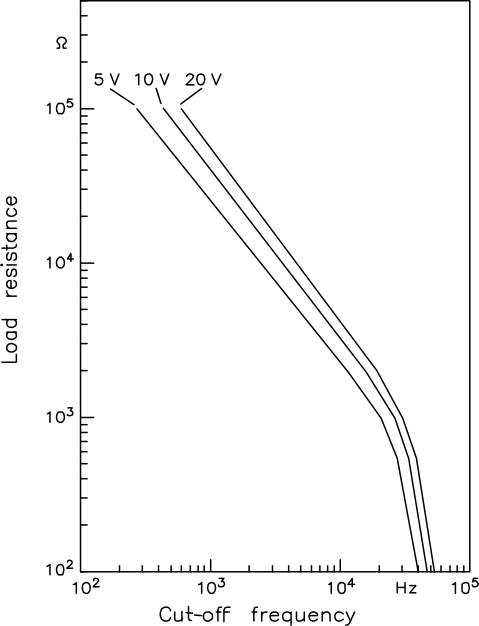
\includegraphics[width=0.5\textwidth]{reflex_cutoff-frequency.png}
    \end{center}

    \fullcite[5]{vishay02:cutoff-frequency}
\end{figure}


\subsubsection{Θερμοκρασία}
Η αύξηση θερμοκρασίας επηρεάζει την απόδοση τόσο της διόδου εκπομπής υπερύθρων,
η οποία μειώνεται, όσο και του φωτοτρανζίστορ, η οποία αυξάνεται
\parencite{vishay06}. Ωστόσο, όπως προκύπτει από το σχήμα
\ref{fig:reflex:t-amb_ctr-rel}, για θερμοκρασίες από 0°C έως 90°C, το
συνολικό αποτέλεσμα επηρεάζεται ελάχιστα. Θα μπορούσε, είτε να αγνοηθεί
πλήρως είτε να συμπεριληφθεί ως σταθερή μείωση του σχετικού λόγου μεταφοράς
ρεύματος.

\begin{figure}
    \caption{Σχέση θερμοκρασίας και Σχετικού λόγου μεταφοράς ρεύματος.
    \label{fig:reflex:t-amb_ctr-rel}}
    \begin{center}%
    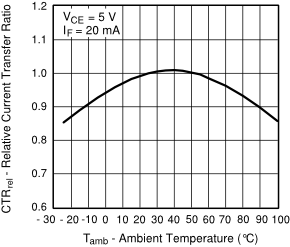
\includegraphics[width=0.5\textwidth]{reflex_t-amb_ctr-rel.png}
    \end{center}

    \fullcite[3]{vishay09:test-circuit}
\end{figure}


\subsubsection{Ένταση πομπού}

Η ένταση των εκπεμπόμενων ακτίνων εξαρτάται από κάποια χαρακτηριστικά κατασκευής
του αισθητήρα (όπως φακός εστίασης) και την ένταση ρεύματος της διόδου
υπερύθρων.
Αφενός, η δίοδος πρέπει να διαρρέεται από ρεύμα ορθής φοράς ελάχιστης έντασης
5mA ώστε να σταθεροποιείται η έξοδός της, αφετέρου, να μην ξεπερνά τη μέγιστη
αποδεκτή τιμή \parencite{vishay02}. Σύμφωνα με τις απόλυτες μέγιστες τιμές του
αισθητήρα TCRT5000, η μέγιστη ένταση ρεύματος ορθής φοράς, $I_F$, είναι 60mA, σε
θερμοκρασία περιβάλλοντος χώρου, $T_{amb}$, 25°C \parencite{vishay09}.

Παρόλο που η εφαρμογή της μέγιστης δυνατής έντασης παρέχει ισχυρότερο σήμα στο
δέκτη λόγω του υψηλότερου συντελεστή σύζευξης (σχήμα \ref{fig:reflex:i-f_ctr})
προτιμάται η εφαρμογή κατά πολύ χαμηλότερης. Στους λόγους συγκαταλέγεται η
τήρηση αποδεκτής έντασης ρεύματος σε περιβάλλον κυμαινόμενης θερμοκρασίας κυρίως
για την επιμήκυνση της διάρκειας ζωής του πομπού. Επίσης, στο ίδιο σχήμα
παρατηρείται ότι ο συντελεστής σύζευξης πλησιάζει ένα ανώτατο όριο 6\% για ρεύμα
ορθής φοράς στο εύρος 35--60mA. Επομένως, επιλέγεται να χρησιμοποιηθεί ρεύμα
ορθής φοράς έως και 35mA.

\begin{figure}
    \caption{Σχέση Ρεύματος ορθής φοράς και Λόγου μεταφοράς ρεύματος.
    \label{fig:reflex:i-f_ctr}}
    \begin{center}%
    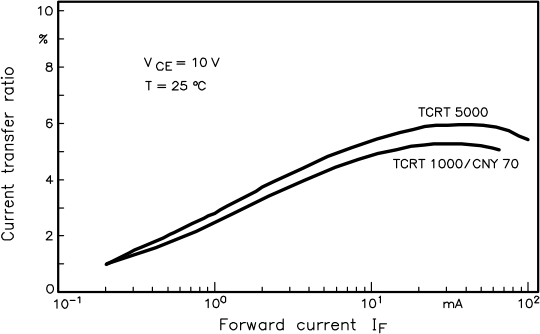
\includegraphics[width=0.8\textwidth]{reflex_i-f_ctr.png}
    \end{center}

    \fullcite[5]{vishay02:forward-current_ctr}
\end{figure}


\subsection{Λοιπές παράμετροι}
\label{subsec:reflex:other-parameters}


\subsubsection{Ρεύμα ηρεμίας}

Ένα φωτοτρανζίστορ διαρρέεται από ρεύμα ακόμα και όταν αυτό βρίσκεται πλήρως
απομονωμένο από φωτεινές πηγές. Το ρεύμα αυτό αναφέρεται ως ρεύμα ηρεμίας
\index{ρεύμα ηρεμίας} (dark current) και επηρεάζεται από την τιμή της
τάσης συλλέκτη-εκπομπού, $V_{CE}$, και, σε μεγαλύτερο βαθμό, από τη θερμοκρασία
\parencite{vishay06}. Τυπική τιμή ρεύματος ηρεμίας, $I_{CEO}$, για τον αισθητήρα
TCRT5000 είναι τα 10nA στα 20V \parencite{vishay09}.

Κρίνεται σκόπιμο να αγνοηθεί στο σχεδιασμό εφόσον προκύψει από τους υπολογισμούς
ότι το ρεύμα ηρεμίας έντασης περίπου 5μA που προκαλείται από την εφαρμογή
τάσης 10V σε μία οριακή θερμοκρασία, $T_{amb}$, 100°C, επηρεάζει ελάχιστα την
έξοδο του αισθητήρα (σχήμα \ref{fig:reflex:t-amb_i-ceo}).

\begin{figure}
    \caption{Σχέση θερμοκρασίας και Ρεύματος ηρεμίας.
    \label{fig:reflex:t-amb_i-ceo}}
    \begin{center}%
    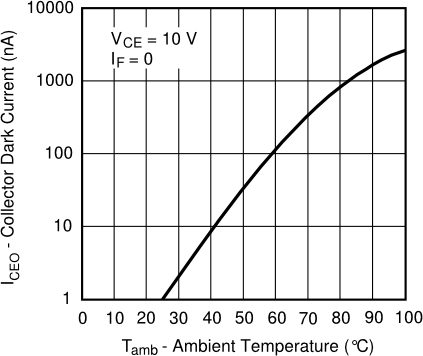
\includegraphics[width=0.5\textwidth]{reflex_t-amb_i-ceo.png}
    \end{center}

    \fullcite[3]{vishay06:dark-current}
\end{figure}


\subsubsection{Οπτικές παρεμβολές}

Σύμφωνα με τον οδηγό \textcite{vishay06}, είναι δυνατό να διοχετεύονται
εκπεμπόμενες ακτίνες από τον πομπό στο δέκτη απευθείας μέσα από την ίδια τη θήκη
καθώς και δια μέσω επιφανειών που περιβάλλουν τον αισθητήρα, πέραν της
ανακλαστικής επιφάνειας, με αποτέλεσμα να προκύπτει ένταση ρεύματος συλλέκτη.

Επιπλέον, σταθερή απευθείας πρόσπτωση φωτός στο φωτοτρανζίστορ μειώνει την
ευαισθησία του, δυνατό φως είναι δυνατό να το κρατήσει μονίμως ενεργό, ενώ
μεταβαλλόμενο, να προκαλέσει αδικαιολόγητη εναλλαγή στο σήμα εξόδου
\parencite{vishay06}.
Ο επιλεγμένος αισθητήρας διαθέτει προστατευτικά φίλτρα τα οποία παρεμποδίζουν το
ορατό φως \parencite{vishay09}. Ωστόσο, ένα μεγάλο εύρος του ηλιακού φωτός
αποτελείται από υπέρυθρες και, συνεπώς, η παράμετρος πρέπει να ληφθεί υπόψη κατά
το σχεδιασμό του συστήματος.

Η περίπτωση παρεμβολών που οφείλονται στην κατασκευή του αισθητήρα είναι δυνατό
να απαλειφθούν καταμετρώντας το σήμα του αισθητήρα σε πλήρη απομόνωσή του και
λαμβάνοντάς το υπόψη, ως σταθερά, κατά την κανονική λειτουργία του κωδικοποιητή.
Ο βαθμός στον οποίο επηρεάζουν οι περιβάλλουσες επιφάνειες μπορεί να εντοπιστεί
με παρόμοιο τρόπο. Ο βαθμός στον οποίο επηρεάζουν οι επικρατούσες συνθήκες
φωτισμού είναι, σαφώς, μεταβλητός και η ίδια προσέγγιση μη εφαρμοστέα. Ωστόσο,
είναι δυνατό να περιοριστεί απομονώνοντας εξωτερικά ολόκληρο τον κωδικοποιητή,
δηλαδή αισθητήρα και ανακλαστική επιφάνεια.


\subsubsection{Θερμοκρασία}

Σε προηγούμενη παράγραφο, μελετήθηκε πώς επηρεάζει η θερμοκρασία το συντελεστή
σύζευξης. Ωστόσο, η θερμοκρασία θέτει και ορισμένα άλλα ζητήματα προς μελέτη.

Η αύξηση θερμοκρασίας της διόδου, ως άμεσο υποπροϊόν της κατανάλωσης ισχύος,
παίζει καθοριστικό ρόλο στον προσδιορισμό της έντασης ρεύματος της διόδου.
Σύμφωνα με το εγχειρίδιο χρήσης τους αισθητήρα \parencite{vishay09}, η μέγιστη
επιτρεπτή τιμή ρεύματος ορθής φοράς του πομπού, $I_F$, ανέρχεται στα 60mA σε
θερμοκρασία περιβάλλοντος χώρου, $T_{amb}$, 25°C. Επιπλέον, καθώς η θερμοκρασία
αυξάνεται, το μέγιστο επιτρεπτό όριο μειώνεται.
Το σχήμα \ref{fig:reflex:power-dissipation} δίνει την απόλυτη μέγιστη τιμή
κατανάλωσης ισχύος σε σχέση με τη θερμοκρασία. Λαμβάνοντας υπόψη ότι $P = VI$,
είναι δυνατό να υπολογιστεί το μέγιστο επιτρεπτό ρεύμα ορθής φοράς βάσει των
διακυμάνσεων της θερμοκρασίας χώρου και της εφαρμοζόμενης τάσης της υλοποίησης.

\begin{figure}
    \caption{Σχέση Κατανάλωσης ισχύος και Θερμοκρασίας.
    \label{fig:reflex:power-dissipation}}
    \begin{center}%
    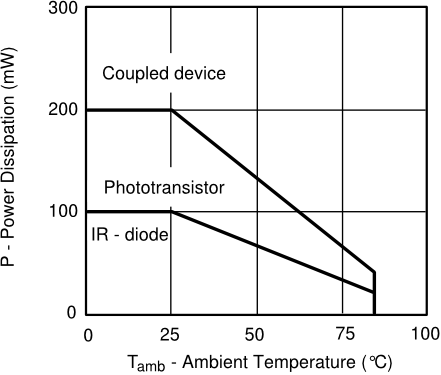
\includegraphics[width=0.5\textwidth]{reflex_power-dissipation.png}
    \end{center}

    \fullcite[3]{vishay09:power-dissipation}
\end{figure}

Κρίνεται αναγκαία η τήρηση χαμηλών θερμοκρασιών στη δίοδο για την επιμήκυνση της
ζωής της και, συνεπώς, του ίδιου του αισθητήρα, καθώς χαμηλή θερμοκρασία
συνεπάγεται ελάχιστη ή καθόλου φθορά της ένωσης p-n της διόδου. Προς επίτευξη
αυτού, η παρεχόμενη ένταση ρεύματος της διόδου είναι κατά πολύ μικρότερη από τη
μέγιστη αποδεκτή, κατάλληλη ακόμα και για θερμοκρασίες που ξεπερνούν τις
απαιτήσεις της υλοποίησης. Επίσης, ο αισθητήρας τίθεται σε λειτουργία μόνο για
τα διαστήματα περιστροφής του άξονα κίνησης, ώστε ο χρόνος κατανάλωσης ενέργειας
με αποτέλεσμα την εκπομπή θερμότητας και αύξηση της θερμοκρασίας τοπικά του
αισθητήρα να είναι περιορισμένος.


\subsection{Υπολογισμοί}
\label{subsec:reflex:calculations}


Σε αυτό το σημείο, επιχειρείται να προσδιοριστούν οι επακριβείς τιμές των
στοιχείων για τη σύνδεση του αισθητήρα υπέρυθρων και των τελικών προδιαγραφών
του κωδικοποιητή, λαμβάνοντας υπόψη τις παραμέτρους που έχουν ήδη περιγραφεί.

Μία βασική ανάγκη είναι η εκτίμηση της έντασης ρεύματος του συλλέκτη, ${I_C}$, η
οποία εξαρτάται από το ρεύμα ορθής φοράς, $I_F$, και το συντελεστή σύζευξης,
$k$.
\begin{equation}
I_C = k \cdot I_F \label{eq:reflex:i-c}
\end{equation}

Ο συντελεστής σύζευξης εξαρτάται από το ρεύμα ορθής φοράς και η σχέση τους
περιγράφεται από το σχήμα \ref{fig:reflex:i-f_ctr}. Ωστόσο, το σχήμα αυτό
αναφέρεται στη χρήση της
λευκής όψης κάρτας Kodak neutral σε λειτουργική απόσταση μέγιστης απόδοσης.

Στην υλοποίηση χρησιμοποιούνται διαφορετικά υλικά ως ανακλαστικές επιφάνειες
και, ενδεχομένως, διαφορετική λειτουργική απόσταση. Ο πραγματικός συντελεστής
σύζευξης για κάθε υλικό και λειτουργική απόσταση προκύπτει από την
\begin{equation}
k = I_{Crel} \cdot k_{Kodak} \label{eq:reflex:k}
\end{equation}
όπου $I_{Crel}$, η σχετική τιμή ρεύματος του συλλέκτη ως αποτέλεσμα του
ανακλαστικού υλικού, της λειτουργικής απόστασης και λοιπών παραμέτρων και
$k_{Kodak}$, ο συντελεστής σύζευξης με χρήση της κάρτας Kodak neutral.

%Προκειμένου να συνεχίσουν οι υπολογισμοί είναι απαραίτητο να επιλεγεί το ρεύμα
%ορθής φοράς.

Το ρεύμα ορθής φοράς, $I_F$, είναι επιθυμητό να επιλεγεί ώστε να μεγιστοποιείται
ο συντελεστής σύζευξης, $k$, και προκύπτει ότι για τον επιλεγμένο αισθητήρα,
TCRT5000, παρατηρείται για ρεύμα ορθής φοράς περίπου 35mA (σχήμα
\ref{fig:reflex:i-f_ctr}).
Ωστόσο, λαμβάνοντας υπόψη το σχήμα \ref{fig:reflex:power-dissipation} και την
ανάγκη για τήρηση χαμηλής κατανάλωσης ισχύος με εφαρμογή ορθής τάση
$V_F = 1.25$V στη δίοδο IR, αντί αυτού, επιλέγεται ρεύμα ορθής φοράς
\begin{equation}
I_F = 20\text{mA} \label{eq:reflex:i-f_value}
\end{equation}
με
\begin{equation}
k_{Kodak} = 5.5\% \label{eq:reflex:k_kodak-value}
\end{equation}

%Όπως προκύπτει από το σχήμα
%[\underline{REF}], %\ref{fig:reflex:ctr},
%για τον επιλεγμένο αισθητήρα, TCRT5000, ο μέγιστος λόγος μεταφοράς ρεύματος, ή
%συντελεστής σύζευξης, είναι 6\%. Ωστόσο, αναφέρεται στη χρήση της λευκής όψης
%κάρτας Kodak neutral, $k_{Kodak}$, σε λειτουργική απόσταση μέγιστης απόδοσης.

Έχει σημειωθεί ότι, εκτός και εάν προκύψει κάποια ιδιαίτερη ανάγκη, η
λειτουργική
απόσταση, $d$, του αισθητήρα επιλέγεται ώστε ο συντελεστής σύζευξης να ευνοείται
κατά το μέγιστο. Επομένως, από το σχήμα \ref{fig:reflex:working-diagram},
προκύπτει ότι
\begin{equation}
d = 2.5 \text{mm}
\end{equation}

Από το σχήμα \ref{fig:reflex:d_switching-distance} προκύπτει ότι για την
επιλεγμένη λειτουργική απόσταση (2.5mm), το ελάχιστο επιτρεπτό διάστημα
εναλλαγής είναι περίπου 2mm. Αφήνοντας περιθώριο σφάλματος, επιλέγεται διάστημα
εναλλαγής
\begin{equation}
X_d = 4 \text{mm}
\end{equation}

Στην υλοποίηση χρησιμοποιείται τυπογραφικό χαρτί ως επιφάνεια με υψηλό
συντελεστή σύζευξης, $k_H$, και φωτοτυπικό μελάνι ως επιφάνεια με χαμηλό
συντελεστή, $k_L$.
Λαμβάνοντας υπόψη τον πίνακα ανακλαστικών υλικών
(πίνακας \ref{tab:reflex:materials}), το
λειτουργικό διάγραμμα για απόσταση $d = 2.5$mm
(σχήμα \ref{fig:reflex:working-diagram}β) και τη σχέση
\eqref{eq:reflex:k_kodak-value}, αντικαθιστώντας στη σχέση \eqref{eq:reflex:k},
προκύπτει ότι
\begin{equation}
k_H = 94 \% \cdot 5.5 \% = 5.17 \%
\end{equation}
\begin{equation}
k_L = 7 \% \cdot 5.5 \% = 0.385 \%
\end{equation}

Με γνωστούς τους συντελεστές σύζευξης $k_H$ και $k_L$ των δύο επιφανειών και το
ρεύμα ορθής φοράς (σχέση \eqref{eq:reflex:i-f_value}), είναι πλέον δυνατός ο
υπολογισμός των αντίστοιχων τιμών της έντασης ρεύματος του συλλέκτη,
αντικαθιστώντας στη σχέση \eqref{eq:reflex:i-c}
\begin{equation}
I_{C_H} = 5.17\% \cdot 20 \text{mA} = 1.034 \text{mA}
\end{equation}
\begin{equation}
I_{C_L} = 0.385\% \cdot 20 \text{mA} = 0.077 \text{mA}
\end{equation}

Αφήνοντας ένα περιθώριο 10\% για μειωμένη απόδοση της διόδου IR ως αποτέλεσμα
φθοράς από την πάροδο χρόνου και ένα 10\% λόγω μεταβολών στη θερμοκρασία
στο εύρος 0--90°C (σχήμα \ref{fig:reflex:t-amb_ctr-rel}), η ένταση ρεύματος του
συλλέκτη ως αποτέλεσμα των υπερύθρων αναπροσαρμόζεται σε $I_{C_H} = 0.827$mA.

% Crosstalk και ambient light
Για το εύρος θερμοκρασιών που ενδιαφέρει, το ρεύμα ηρεμίας είναι περίπου
1$\mu$A (0--90°C, σχήμα \ref{fig:reflex:t-amb_i-ceo}) και αμελητέο για της
ανάγκες της υλοποίησης.

Όπως προκύπτει από τους υπολογισμούς, η ένταση ρεύματος του συλλέκτη κυμαίνεται
εντός μερικών εκατοντάδων $\mu$A, ενώ, κύριο ενδιαφέρον είναι το πλήθος των
μεταβολών και όχι η ανίχνευση της πραγματικής τιμής της ένταση.
Σύμφωνα με δελτίο των \textcites{optek04}{fairchild02}, το φωτοτρανζίστορ είναι
δυνατό να χρησιμοποιηθεί ως διακόπτης (switch mode) όπου το παραγόμενο σήμα του
ενισχύεται και ανάγεται σε δυαδικό ψηφίο προσαρμόζοντας μόνο την αντίσταση
φόρτου, χωρίς να απαιτείται χρήση επιπρόσθετων ηλεκτρονικών διατάξεων, ως
ακολούθως
\begin{equation}
R_L > \frac{V_{CC} - V_{CEsat}}{I_C} \label{eq:reflex:r-l}
\end{equation}
όπου $V_{CC}$ η τάση της πηγής, $V_{CEsat}$ η τάση κορεσμού συλλέκτη-εκπομπού
και $I_C$ η ένταση ρεύματος του συλλέκτη. Με αυτόν τον τρόπο, το φωτοτρανζίστορ
παραμένει αποκομμένο παράγοντας τάση περίπου 0.8V (λογικό 0), έως ότου κορεστεί
από τις προσπίπτουσες ακτίνες ώστε να παρέχει περίπου την τάση της πηγής
(λογικό 1) \parencite{fairchild02}.

Αντικαθιστώντας $V_{CC} = 5 V$, $V_{CEsat} = 0.4 V$ και $I_C = 0.8 mA$ στην
ανίσωση \eqref{eq:reflex:r-l} προκύπτει ότι η αντίσταση φόρτου πρέπει να είναι
$R_L > 5.75$k$\Omega$. Σημειώνεται ότι για την αλλαγή της εξόδου του ενισχυτή
χρησιμοποιείται τιμή χαμηλότερη της $I_{CH}$ ώστε για ένταση ρεύματος από την
τιμή αυτήν και πάνω να παράγεται η υψηλή έξοδος του ενισχυτή.

Η διάμετρος του άξονα στο ύψος του αισθητήρα είναι 0.42in. Επομένως, η
περιφέρεια άξονα και, συνεπώς το μήκος της ταινίας κωδικοποίησης είναι
\begin{equation}
C = \pi{}d \approx 3.35 \text{cm}
\end{equation}

Διάστημα εναλλαγής 4mm σε αυτό το μήκος ταινίας δημιουργεί
$\frac{C}{X_d} \approx \frac{3.35}{0.4} \cdot \frac{\text{cm}}{\text{cm}}
\approx 8.37$ τμήματα
ταινίας. Το πλήθος των τμημάτων που καλύπτουν την περιφέρεια του άξονα πρέπει να
είναι άρτιος αριθμός ώστε να αποτελούν μία συνέχεια καθώς ο άξονας ολοκληρώνει
μία πλήρη περιστροφή και ξεκινάει την επόμενη. Επομένως, τα τμήματα επιλέγονται
να είναι 8 και βάσει αυτού, υπολογίζεται νέο διάστημα εναλλαγής
$X_d = \frac{C}{8} \approx 0.42$cm.

Εφόσον η αντίσταση φόρτου έχει υπολογιστεί και είναι γνωστό και το πλήθος των
εναλλαγών, ανάγεται η συχνότητα αποκοπής περίπου 6kHz ($R_L = 6.9$k$\Omega$ για
$V_{CC} = 5$V, σχήμα \ref{fig:reflex:cutoff-frequency}). Με κάθε πλήρη
περιστροφή του άξονα, προκαλούνται 8 εναλλαγές ενώ επιτρέπονται κατά το μέγιστο
6000 εναλλαγές το δευτερόλεπτο. Επομένως, ένα μέγιστο υπολογίζεται στα
$\frac{6000}{8} \cdot
\frac{
    \frac{\text{εναλλ}}{\text{sec}}
}{
\frac{\text{εναλλ}}{\text{rev}}} = 750 \text{rps}$, υπερβολικά υψηλό για τις
απαιτήσεις της υλοποίησης.


\chapter{Υποσύστημα κίνησης}
\label{ch:motor}

Στο κεφάλαιο Κατασκευή (σ.~\pageref{ch:construction}) αναλύθηκαν τα συστατικά
στοιχεία και οι επιμέρους διατάξεις που συνθέτουν τη φυσική υπόσταση της
συσκευής, μέρος του οποίου είναι αφιερωμένο στους
άξονες κίνησης. Όπως αναφέρεται σε εκείνο το κεφάλαιο, οι μετρήσεις
πραγματοποιούνται από ένα κινητό εξάρτημα της συσκευής, την κεφαλή, που
μετακινείται στο χώρο που ορίζουν αυτοί οι τρεις, στον αριθμό, άξονες.

\begin{figure}
    \caption{Υποσύστημα κίνησης.\label{fig:motor:lvl-0}}
    \begin{center}
    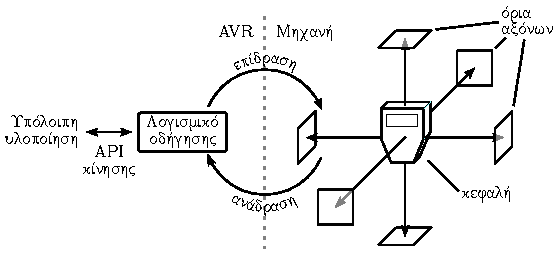
\includegraphics{drive_lvl-0}
    \end{center}
\end{figure}

Στο παρόν κεφάλαιο αναλύεται η διασύνδεση του μικροελεγκτή με τους κινητήρες και
συμπληρωματικές ηλεκτρονικές και μηχανικές διατάξεις για την ανάπτυξη ενός
συστήματος ελέγχου της μετατόπισης της κεφαλής (βλ. σχήμα
\ref{fig:motor:lvl-0}).

Τρεις σερβοκινητήρες συνεχούς περιστροφικής κίνησης (εφεξής, κινητήρες) -- ένας
για κάθε άξονα -- χρησιμοποιούνται για την παραγωγή κίνησης με γωνιακή ταχύτητα
που ελέγχεται μέσω ενός σήματος από παλμούς κυμαινόμενου πλάτους, την
αναφερόμενη ως διαμόρφωση PWM (\te{Pulse-Width Modulation}). Μέσω της χρήσης
απλών μηχανών (\te{simple machine}), η περιστροφική κίνηση μετατρέπεται σε
γραμμική κίνηση της κεφαλής.
Τα υπόλοιπα συστήματα της υλοποίησης αντιλαμβάνονται και χειρίζονται τη θέση
της κεφαλής μέσω συντεταγμένων τριών συνιστωσών (X, Y και Z) που κυμαίνονται
εντός συγκεκριμένων ορίων (\nameref{sec:motor:coordinates} σ.~%
\pageref{sec:motor:coordinates}).
% Something more on PWM (such as averaging voltage).
Αρχικά, αναλύονται
τα διαθέσιμα κυκλώματα Χρονομετρητών\slash{}Απαριθμητών (\te{Timer\slash{}%
Counter}) του μικροελεγκτή που υποστηρίζουν παραγωγή σήματος PWM και
συγκρίνονται τα χαρακτηριστικά τους σε σχέση με τις απαιτήσεις των κινητήρων και
της υλοποίησης προκειμένου να επιλεγεί και διευθετηθεί το πλέον κατάλληλο
(\nameref{sec:motor:motion} σ.~\pageref{sec:motor:motion}).

% (Διευθέτηση γεννήτριας PWM)
% Κάτι σχετικό με κύκλο εργασίας; ???
% PWM για την παραγωγή μίας μέσης τάσης που μετατρέπεται (από τον κινητήρα)

Εν συνεχεία, στην ενότητα Δρομολόγηση (σ.~\pageref{sec:motor:routing})
αναφέρεται η βασική ανάγκη για πολύπλεξη ορισμένων γραμμών ελέγχου, όπως οι
γραμμές σήματος PWM, ώστε να είναι δυνατό να υποστηριχθούν και οι τρεις
κινητήρες μέσω του περιορισμένου αριθμού ακροδεκτών που δύνανται να παράγουν
σήμα PWM.
Στην ενότητα Διεκπεραίωση (σ.~\pageref{subsec:motor:autoshut}) περιγράφεται η
ανάπτυξη ενός μηχανισμού που επιτρέπει το ίδιο το υλικό του μικροελεγκτή να
σταματά την κίνηση των κινητήρων όταν ολοκληρώνεται μία προκαθορισμένη
μετατόπιση, ώστε να εξασφαλίζεται ότι η κεφαλή ακινητοποιείται ακόμα και εάν τη
στιγμή εκείνη, η CPU του μικροελεγκτή είναι απασχολημένη με άλλες εργασίες.
Στην ίδια ενότητα παρουσιάζεται πώς, τελικά, επιτυγχάνεται ταυτόχρονη κίνηση της
κεφαλής στο επίπεδο X-Y (\nameref{ssubsec:motor:common-translation} σ.~%
\pageref{ssubsec:motor:common-translation}).

\begin{figure}
    \caption{\label{fig:motor:lvl-1}}
    \begin{center}
    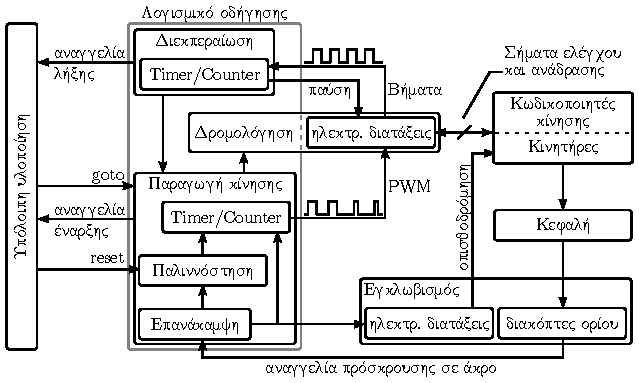
\includegraphics{drive_lvl-1}
    \end{center}
\end{figure}

Το κεφάλαιο ολοκληρώνεται με την περιγραφή ορισμένων συμπληρωματικών
μηχανισμών, του Εγκλωβισμού και επανάκαμψης (σ.~\pageref{sec:motor:backtrack})
και της Παλιννόστησης (σ.~\pageref{subsec:motor:homing}). Ο μηχανισμός του
εγκλωβισμού προφυλάσσει τη συσκευή
από την πρόκληση βλαβών, κυρίως στους κινητήρες, επιβάλλοντας την ακινητοποίησή
της όταν
η κεφαλή προσκρούει στα άκρα της συσκευής. Λόγω της κρισιμότητας της λειτουργίας
του, ο εγκλωβισμός υλοποιείται σε μηχανικό επίπεδο με χρήση ανασταλτικών
διακοπτών. Οι διακόπτες χρησιμοποιούνται ως έναυσμα για το λογισμικό το οποίο,
με τη σειρά του, προκαλεί την επαναφορά της κεφαλής σε μία γνωστή θέση (τη θέση
επιστροφής) (βλ. Παλιννόστηση σ.~\pageref{subsec:motor:homing}).
Επιπλέον περιγράφεται πώς η συσκευή αποπειράται εκ νέου, και για μία μόνο ακόμη
φορά, τη μετακίνηση στη θέση που είχε προηγουμένως προκαλέσει εγκλωβισμό. Αυτό
συμβαίνει ώστε να εξαλείφεται το ενδεχόμενο ότι ο εγκλωβισμός οφειλόταν σε
αδυναμία παρακολούθησης της πραγματικής θέσης της κεφαλής (αστοχία υλικού) και
που ίσως πλέον καταστεί δυνατό λόγω της πρόσφατης επαναφοράς της κεφαλής στη
θέση επιστροφής (λειτουργία επανάκαμψης).

Η λογική συσχέτιση μεταξύ των μονάδων του υποσυστήματος κίνησης περιγράφεται από
το σχήμα \ref{fig:motor:lvl-1} ενώ η ανάλυσή τους πραγματοποιείται στις επόμενες
ενότητες.

%
% Κινητήρες
%
%\section{Κινητήρες}

\section{Συντεταγμένες και Λειτουργικό εύρος}
\label{sec:motor:coordinates}

Τρεις άξονες γραμμικής κίνησης χρησιμοποιούνται για τη μετακίνηση της κεφαλής
πάνω από την επιφάνεια του παρακολουθούμενου υλικού και κατακορύφως προς και από
αυτό για την πραγματοποίηση μετρήσεων.
Οι άξονες υποδιαιρούνται σε ένα πλήθος νοητών διακριτών θέσεων στις οποίες
μπορεί να μεταβεί η κεφαλή. Το πλήθος αυτών των θέσεων εξαρτάται από την
ελάχιστη δυνατή μετατόπιση που μπορεί να διανύσει η κεφαλή καθώς και το συνολικά
διαθέσιμο μήκος των αντίστοιχων ραγών της συσκευής (πάνω στις οποίες κινείται η
κεφαλή). Στο πλαίσιο της υλοποίησης, η ελάχιστη μετατόπιση ορίζεται ως μία
πλήρης περιστροφή του κινητήρα του αντίστοιχου άξονα. Πρακτικά, αυτό συνεπάγεται
μετατοπίσεις των 4cm, περίπου. Επιπλέον, επιλέγεται να υποστηρίζεται ένα μέγιστο
πλήθος 255 μετατοπίσεων ανά άξονα, δηλαδή ένα μέγιστο μήκος 1km ανά ράγα.

Σε κάθε περίπτωση, το διαθέσιμο πλήθος θέσεων της κεφαλής ορίζουν το αναφερόμενο
ως λειτουργικό εύρος του οποίου η μέγιστη τιμή εξαρτάται άμεσα από τις
διαστάσεις των ραγών της συσκευής. Ωστόσο, προκειμένου να παρέχεται
μεγαλύτερη ευελιξία, το υποσύστημα κίνησης είναι δυνατό να διευθετείται δυναμικά
μέσω λογισμικού ώστε να λειτουργεί σε ένα προσαρμοσμένο λειτουργικό εύρος,
υποσύνολο του μέγιστου δυνατού (βλ. \nameref{subsec:network:config} σ.~%
\pageref{subsec:network:config}).
Η δυνατότητα αυτή επιτρέπει την παρακολούθηση μικρότερων επιφανειών από τη
μέγιστη υποστηριζόμενη. Το σχήμα

\begin{figure}
    \caption{Συντεταγμένες και Λειτουργικό εύρος.\label{fig:motor:coordinates}}
    Σημειώνεται ότι οι συνιστώσες των  συντεταγμένων αριθμούνται από το 0, ενώ
    το λειτουργικό εύρος (το οποίο αντιπροσωπεύει μέγεθος διάστασης) από το 1.
    \begin{center}
    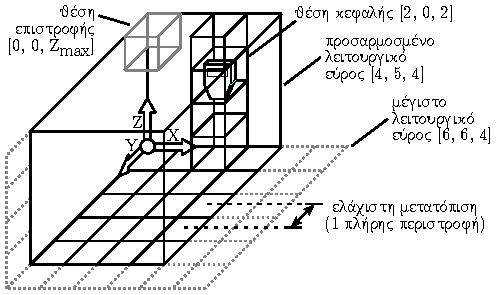
\includegraphics{drive_coordinates}
    \end{center}
\end{figure}

Την κάθε στιγμή, η θέση της κεφαλή προσδιορίζεται από τρεις τιμές· μία για τη
θέση που κατέχει στον άξονα X, μία για τον άξονα Y και μία για το Z, που
συνολικά αναφέρονται ως οι συντεταγμένες (της θέσης) της κεφαλής. Προφανώς,
η κεφαλή μπορεί να τεθεί μόνο σε συντεταγμένες που βρίσκονται εντός του
τρέχοντος λειτουργικού εύρους (είτε αυτό είναι το μέγιστο δυνατό είτε
προσαρμοσμένο).


\section{Παραγωγή κίνησης}
\label{sec:motor:motion}

Σύμφωνα με εγχειρίδιο χρήσης της \textcite{hitec02}, όλοι οι κινητήρες της
λειτουργούν σε τάση 4.8--6V δεχόμενοι τετραγωνικό σήμα ελέγχου με διαμόρφωση
PWM (\textenglish{Pulse-Width Modulation}) 3--5V σε συχνότητα ανανέωσης 50Hz.
Η διάρκεια των παλμών κυμαίνεται μεταξύ 0.9ms και 2.1ms, με παλμούς των 1.5ms να
χρησιμοποιούνται για την ακινητοποίησή τους \parencite{hitec02}.

Οι παραγωγή των παλμών μπορεί να πραγματοποιηθεί είτε με λογισμικό είτε από
κάποιο διαθέσιμο κύκλωμα Χρονομετρητή\slash Απαριθμητή (\textenglish{Timer\slash
Counter}) του μικροελεγκτή. Το κύριο πλεονέκτημα του λογισμικού είναι η
ελευθερία επιλογής οποιουδήποτε ακροδέκτη για την έξοδο του σήματος καθώς και η
δυνατότητα παραγωγής πολλαπλών τέτοιων σημάτων που περιορίζονται από το συνολικό
πλήθος ακροδεκτών ή τη συχνότητα του ρολογιού συστήματος (όποιο είναι
μικρότερο).

Αντιθέτως, στην περίπτωση χρήσης κυκλωμάτων, το παραγόμενο σήμα διοχετεύεται
στους συγκεκριμένους ακροδέκτες με τους οποίους είναι το καθένα εσωτερικά
συνδεδεμένο και, σαφώς, το μέγιστο πλήθος παράλληλων σημάτων περιορίζεται από το
συνολικό αριθμό τέτοιων κυκλωμάτων. Επίσης, κάθε Χρονομετρητής\slash Απαριθμητής
υπόκειται σε πρόσθετους περιορισμούς, όπως το εύρος τιμών που υποστηρίζει ο
καθένας (για παράδειγμα, ανάλυση 8- ή 16-bit).

Ωστόσο, στη χρήση κυκλώματος Χρονομετρητή\slash Απαριθμητή συγκαταλέγονται και
ορισμένα σημαντικά πλεονεκτήματα.
Καθότι το σήμα παράγεται από ξεχωριστό κύκλωμα, η CPU του μικροελεγκτή είναι
διαθέσιμη για την εκτέλεση οποιασδήποτε άλλης εργασίας (για παράδειγμα, κάποιας
ρουτίνας εξυπηρέτησης διακοπής) παράλληλα με την παραγωγή του σήματος, χωρίς να
απαιτείται πολύπλεξη εργασιών (ώστε να αποδίδονται κβάντα τόσο στη γεννήτρια
σήματος όσο και σε κάποια άλλη εργασία). Ένα δεύτερο, λιγότερο σημαντικό για την
προκειμένη υλοποίηση, πλεονέκτημα είναι η δυνατότητα επίτευξης υψηλότερων
συχνοτήτων με πολύ λιγότερο θόρυβο (\textenglish{jitter}) και μεγαλύτερη
ακρίβεια.

Τελικά, για την παραγωγή σήματος PWM των κινητήρων επιλέγεται η χρήση κυκλώματος
Χρονομετρητή\slash Απαριθμητή καθώς, επιπροσθέτως των ανωτέρω πλεονεκτημάτων,
παρουσιάζει υψηλότερο ενδιαφέρον, από εκπαιδευτικής πλευράς.


\subsection{Γεννήτρια PWM}

Ο μικροελεγκτής ATmega328P διαθέτει δύο κυκλώματα Χρονομετρητή\slash Απαριθμητή
με δυνατότητα παραγωγής σήματος PWM. Ο πρώτος (Timer\slash Counter0) είναι 8-bit
και ο δεύτερος (Timer\slash Counter1), 16-bit. Για την επιλογή κάποιου, κρίνεται
σκόπιμη η περαιτέρω ανάλυση της λειτουργίας της γεννήτριας PWM καθώς και των
απαιτήσεων για το σήμα ελέγχου των κινητήρων.

Όσον αφορά τη γεννήτρια PWM, ο Χρονομετρητής\slash Απαριθμητής διαθέτει έναν
καταχωρητή μετρητή, τον TCNTn, ο οποίος σταδιακά αυξάνεται. Επίσης, διαθέτει
δύο ακόμα καταχωρητές, τους OCRnA και OCRnB, οι οποίοι αντιστοιχίζονται με
ακροδέκτες του μικροελεγκτή, αναφερόμενοι ως OCnA και OCnB. Μόλις η τιμή του
TCNTn γίνει ίση με την τιμή που περιέχεται είτε στον OCRnA είτε στον OCRnB,
είναι δυνατή η αλλαγή της εξόδου του αντίστοιχου ακροδέκτη. Ο TCNTn συνεχίζει
την ανοδική του πορεία έως ότου φτάσει την τιμή TOP. Από το σημείο αυτό και
ανάλογα με τη λειτουργία που έχει επιλεγεί, ο TCNTn είτε επανέρχεται ακαριαία
στην τιμή 0 και αρχίζει εκ νέου τον επόμενο κύκλο, είτε φθίνει σταδιακά μέχρι το
0, πάντα εναλλάσσοντας την τιμή των OCnA και OCnB όποτε εξισώνεται με τους OCRnA
και OCRnB, αντιστοίχως \parencite[100--102,124--129]{atmel13}.
Γίνεται αντιληπτό ότι η συχνότητα με την οποία αυξάνεται ο TCNTn καθώς και η
τιμή TOP επηρεάζουν τη συχνότητα του παραγόμενου σήματος. Παράλληλα, η τιμή των
OCRnA και OCRnB επηρεάζουν τον κύκλο εργασίας του (\textenglish{duty cycle}),
δηλαδή το τμήμα της περιόδου κατά το οποίο το παραγόμενο σήμα βρίσκεται σε
λογικό 1.

Η παραγωγή PWM υποστηρίζεται από τρεις ρυθμίσεις λειτουργίας των
Χρονομετρητών\slash Απαριθμητών, τις \textenglish{Fast PWM mode, Phase Correct
PWM mode (PCPWM)} και \textenglish{Phase and Frequency Correct PWM mode
(PFCPWM)}, εκ των οποίων οι δύο τελευταίες ενδείκνυνται για τον έλεγχο κινητήρων
εν γένει, και αυτό επειδή το παραγόμενο σήμα ανταποκρίνεται πιο ομαλά στις
αλλαγές της τιμής TOP \parencite[126,128]{atmel13}. Οι PCPWM και PFCPWM, εφόσον
η τιμή TOP -- η τιμή μέχρι την οποία αυξάνει ο TCNTn πριν αρχίσει τη φθίνουσα
πορεία του -- διατηρείται σταθερή κατά τη διάρκεια λειτουργίας του μετρητή,
είναι πανομοιότυπες \parencite[127]{atmel13}. Στην περίπτωση της υλοποίησης, η
συχνότητα του παραγόμενου σήματος είναι σταθερή, όπως έχει αναφερθεί, στα 50Hz
και, συνεπώς, το ίδιο ισχύει για την τιμή TOP. Ως αποτέλεσμα, οι λειτουργίες
PCPWM και PFCPWM είναι ισοδύναμες για τις ανάγκες της υλοποίησης και μπορεί να
προτιμηθεί είτε η μία είτε η άλλη, στην περίπτωση που επιλεγεί ο
\textenglish{Timer\slash Counter1}, ή η PCPWM, στην περίπτωση που επιλεγεί ο
\textenglish{Timer\slash Counter0}, καθώς σύμφωνα με τις επιλογές παραγωγής
κυματομορφής της \textcite[107]{atmel13}, ο \textenglish{Timer\slash Counter0}
υποστηρίζει μόνο αυτήν.


\subsubsection{Συχνότητα και κύκλος εργασίας}
% \nref : better caption

Στις λειτουργίες PCPWM και PFCPWM, η συχνότητα του παραγόμενου σήματος παρέχεται
από τη σχέση \parencite[102,128,129]{atmel13}:
\begin{equation}
\label{eq:motor:f_pwm}
f_{PWM} = \frac{f_{clk_{I/O}}} {2\;N\;TOP}
\end{equation}

\noindent όπου, \\
\begin{tabu}{X[-1] @{ : }  X}
$f_{clk_{I/O}}$ & Συχνότητα ρολογιού που λαμβάνουν οι μετρητές (καθώς και
                  άλλα περιφερειακά, όπως SPI).                               \\
$N$             & Τιμή υποδιαίρεσης ρολογιού για χρήση από τους μετρητές (1,
                  8, 64, 256 ή 1024).                                         \\
$TOP$           & Η μέγιστη τιμή που παίρνει ο TCNTn.
\end{tabu}

Η συχνότητα ρολογιού, $f_{clk_{I/O}}$, της υλοποίησης ορίζεται στα 4MHz, ενώ
έχει ήδη αναφερθεί η επιθυμητή συχνότητα του παραγόμενου σήματος, $f_{PWM}$,
(50Hz). Η τιμή υποδιαίρεσης, $N$, προσδιορίζεται από τα bit CSn2:0 του
καταχωρητή TCCRnB, και επιτρέπει τη μείωση της συχνότητας των μετρητών. Η χρήση
της τιμής $TOP$ έχει αναφερθεί προηγουμένως. Η τιμή της προσδιορίζεται κατά την
επιλογή της λειτουργίας παραγωγής κυματομορφής μέσω των bit WGM των καταχωρητών
TCCRnA και TCCRnB. Στον πίνακα \ref{tab:motor:wgm} παρουσιάζονται ορισμένες
ρυθμίσεις PCPWM των δύο μετρητών. Σημειώνεται ότι στην περίπτωση του
\textenglish{Timer\slash Counter0}, οι δύο λειτουργίες που αναφέρονται είναι οι
μοναδικές PCPWM, ενώ στην περίπτωση του \textenglish{Timer\slash Counter1},
έχουν παραλειφθεί ορισμένες οι οποίες είναι παρόμοιες με την λειτουργία 1 του
\textenglish{Timer\slash Counter0} (δηλαδή, προκαθορισμένες σταθερές τιμές
0x00FF, 0x01FF και 0x3FF).

\begin{table}
    \caption{Μέρος ρυθμίσεων PCPWM των \textenglish{Timer\slash Counter0} και 1.
        \label{tab:motor:wgm}}

\begin{center}
\begin{tabu} spread 0pt
    {X[-1,C] X[-1,C] X[-1,C] X[-1,C] X[-1,C] X[-1,C] X[-1]}

    \rowfont\bfseries
                    & {Mode} & {WGMn3} & {WGMn2} & {WGMn1} & {WGMn0} & {TOP}  \\
    \tabucline{2-}
    Timer\slash
    Counter0        &      1 &      -- &       0 &       0 &       1 &  0xFF  \\
                    &      5 &      -- &       1 &       0 &       1 & OCR0A  \\
    Timer\slash
    Counter1        &     10 &       1 &       0 &       1 &       0 &  ICR1  \\
                    &     11 &       1 &       0 &       1 &       1 & OCR1A  \\
\end{tabu}

\floatfoot{Απόσπασμα \fullcite[107,133]{atmel13}}
\end{center}\end{table}

Οι λειτουργίες που παρέχουν μία προκαθορισμένη σταθερή τιμή (0xFF\slash 0x00FF,
0x01FF και 0x03FF) απορρίπτονται καθώς, εάν αντικατασταθούν στη σχέση
\eqref{eq:motor:f_pwm}, αποτυγχάνουν να παράξουν μία αποδεκτή τιμή υποδιαίρεσης,
$N$, και, κατ' επέκταση, συχνότητα 50Hz. Οι υπόλοιπες λειτουργίες, οι οποίες
χρησιμοποιούν ως τιμή TOP την τιμή που τίθεται στον αναφερόμενο, κάθε φορά,
καταχωρητή, παρέχουν περισσότερη ευελιξία και ακρίβεια καθώς επιτρέπουν την
αυθαίρετη επιλογή μίας αποδεκτής τιμής $N$ και βάσει αυτής να υπολογιστεί η τιμή
TOP.

Ωστόσο, στην περίπτωση του \textenglish{Timer\slash Counter0}, ο καταχωρητής
στον οποίο εκχωρείται η τιμή TOP μπορεί μόνο να είναι ο OCR0A. Συνεπώς, μόνο ο
ακροδέκτης OC0B μπορεί να χρησιμοποιηθεί ως έξοδος σήματος PWM, ο κύκλος
εργασίας του οποίου ελέγχεται από τον OCR0B. Εάν επιλεγεί αυτή η διευθέτηση του
κυκλώματος θα είναι δυνατό να ελεγχθεί η κίνηση ενός μόνο κινητήρα τη φορά,
κάτι που αποτρέπει την παράλληλη κίνηση σε δύο άξονες. Συνεπώς, προτιμάται η
λειτουργία 10 του \textenglish{Timer\slash Counter1}, η οποία επιτρέπει να
αποστέλλεται σήμα PWM διαφορετικού κύκλου εργασίας δια μέσω του ενός ή και των
δύο ακροδεκτών.


\subsubsection{Διευθέτηση γεννήτριας PWM}

Είναι γνωστό ότι η επιλογή της τιμής υποδιαίρεσης, $N$, μπορεί να γίνει πλέον
αυθαίρετα. Στην πραγματικότητα, εφαρμόζοντας τις διαθέσιμες τιμές που αναφέρει η
\textcite[109]{atmel13} -- 1, 8, 64, 256 και 1024 -- στη σχέση
\eqref{eq:motor:f_pwm}, μόνο οι τρεις πρώτες παράγουν ακέραιο αριθμό. Ωστόσο,
ποια από τις τρεις είναι κατάλληλη;

Στο σημείο αυτό κρίνεται απαραίτητη η λεπτομερέστερη εξέταση των χαρακτηριστικών
των κινητήρων σχετικά με το αναμενόμενο σήμα ελέγχου. Η συχνότητα σήματος 50Hz
συνεπάγεται περιόδους των 20ms, εκ των οποίων, το σήμα ελέγχου βρίσκεται σε
λογικό 1 για 0.9--2.1ms \parencite{hitec02}. Για απλούστευση, θεωρείται εύρος
παλμών 1--2ms, καθώς οι ακραίες τιμές παράγουν τη μέγιστη γωνιακή ταχύτητα που,
ούτως ή άλλως, ξεπερνά τις απαιτήσεις της υλοποίησης. Συνεπώς, ο κύκλος εργασίας
του παραγόμενου σήματος πρέπει να κυμαίνεται μόλις στο 5--10\%. Στον πίνακα
\ref{tab:motor:prescaler} υπολογίζονται, βάσει της σχέσης \eqref{eq:motor:f_pwm}
και για τις τρεις πρώτες διαθέσιμες τιμές υποδιαίρεσης, $N$, η τιμή TOP που
παράγει 50Hz συχνότητα σήματος. Οι στήλες «5\%», «7.5\%» και «10\%» περιέχουν
την τιμή των OCR1x που παράγουν (ή πλησιάζουν, στην περίπτωση όπου $N = 64$) τον
αντίστοιχο κύκλο εργασίας. Οι κύκλοι εργασίας κοντά στο 7.5\% χρησιμοποιούνται
για την ακινητοποίηση του κινητήρα, ενώ οι τιμές μέχρι τα δύο άκρα (5\% και
10\%), αυξάνουν σταδιακά τη γωνιακή ταχύτατα (αριστερόστροφα και δεξιόστροφα,
αντιστοίχως).

\begin{table}
    \caption{Κύκλοι εργασίας και τιμές OCR1x. \label{tab:motor:prescaler}}
\begin{center}
\begin{tabu} spread 0pt {*5{X[-1r]}}

    \rowfont\bfseries
    Υποδιαίρεση &   TOP &      5\% &   7.5\% &   10\%                         \\
    \hline
              1 & 40000 &     2000 &    3000 &   4000                         \\
              8 &  5000 &      250 &     375 &    500                         \\
             64 &   625 &       32 &  46--47 &     62                         \\
\end{tabu}
\end{center}\end{table}

Φαινομενικά, τα αποτελέσματα προτρέπουν τη χρήση υποδιαίρεσης $N = 1$ ώστε να
παρέχεται μεγαλύτερος έλεγχος του κύκλου εργασίας του σήματος. Ωστόσο, στην
πραγματικότητα, οι ερασιτεχνικοί κινητήρες που χρησιμοποιούνται στην υλοποίηση,
ενδεχομένως οι κινητήρες εν γένει, αδυνατούν να διακρίνουν τόσο μικρές
διαφοροποίησεις στο σήμα, που σημαίνει ότι παρότι το εύρος τιμών είναι
μεγαλύτερο, οι περισσότερες τιμές αλληλοκαλύπτονται και προκαλούν την ίδια
συμπεριφορά κινητήρα. Για παράδειγμα, με $TOP = 3001$, ο κύκλος εργασίας είναι
7.5025\%, ενώ με $TOP = 3010$, 7.525\%. Και στις δύο περιπτώσεις -- προφανώς,
και σε όλες τις ενδιάμεσες -- ο κινητήρας παραμένει ακίνητος. Παρόμοια
συμπεριφορά παρουσιάζεται και για μεγαλύτερες γωνιακές ταχύτητες.

Στο αντίθετο άκρο, η χρήση υποδιαίρεσης $N = 64$ παρέχει πολύ λίγο έλεγχο στη
διακύμανση της ταχύτητας· μόλις 14 διακριτές τιμές για κάθε φορά περιστροφής.
Στον πλαίσιο της υλοποίησης επιλέγεται υποδιαίρεση $N = 8$ και οι αντίστοιχες
ρυθμίσεις.

%Ενδεχομένως λιγότερες, αν σκεφτούμε ότι ακόμα και κινητήρες του ίδιου μοντέλου
%μπορεί να διαθέτουν ελαφρώς διαφορετική απόκριση στον ίδιο κύκλο εργασίας.


\section{Δρομολόγηση σημάτων}
\label{sec:motor:routing}

% Κύκλωμα αναμετάδοσης
%

Ο μετρητής \textenglish{Timer\slash Counter1} διευθετείται ώστε να παράγονται
μέχρι δύο σήματα PWM, ανεξαρτήτου κύκλου εργασίας το καθένα αλλά της ίδιας
συχνότητας. Συνεπώς, είναι δυνατός ο ταυτόχρονος χειρισμός μέχρι και δύο
κινητήρων. Ωστόσο, εάν είναι αποδεκτός ο χειρισμός περισσότερων, του ενός,
κινητήρων από την ίδια γραμμή ελέγχου με ενεργοποίηση μόνο του ενός κάθε φορά,
τότε μπορούν να υποστηριχθούν περισσότεροι, με χρήση κάποιου εξωτερικού
κυκλώματος επιλογής του επιθυμητού, όπως για παράδειγμα, ενός αποπολυπλέκτη.

Η υλοποίηση χρησιμοποιεί τρεις κινητήρες, έναν για κάθε άξονα κίνησης, οι οποίοι
συμβολικά ονομάζονται, ανάλογα με τον άξονα που εξυπηρετούν, κινητήρας X,
κινητήρας Y και κινητήρας Z. Οι κινητήρες X και Y μετακινούν την κεφαλή σε
επίπεδο παράλληλο του παρακολουθούμενου υλικού, ενώ ο κινητήρας Z, κατακόρυφα
προς το υλικό, ώστε οι αισθητήρες να διεισδύουν σε κατάλληλο βάθος πριν τη λήψη
μετρήσεων.

Λόγω της φύσεως του υλικού και για την μείωση αντιστάσεων κατά την κίνηση αλλά
και την αποφυγή πιθανών φθορών της κεφαλής ή και των αισθητήρων, εφαρμόζεται
ολική ανύψωση της κεφαλής προτού πραγματοποιηθεί μετακίνηση σε νέα θέση στο
επίπεδο X-Y. Αντιστοίχως, η κεφαλή χαμηλώνεται μόνο όταν οι άλλοι δύο κινητήρες
βρίσκονται σε ηρεμία. Συνεπώς, προκύπτει ότι οι κινητήρες X και Y μπορούν να
είναι ενεργοποιημένοι ταυτόχρονα, ο ένας λαμβάνοντας σήμα από τον ακροδέκτη OC1A
και ο άλλος, από τον OC1B. Ωστόσο, για να συμπεριληφθεί και ο κινητήρας Z, το
σήμα του καθώς και το σήμα ενός εκ των άλλων δύο κινητήρων αποδίδεται πότε στον
έναν και πότε στον άλλο μέσω αποπολυπλέκτη. Το σχήμα
\ref{fig:motor:route_pwm} παρουσιάζει αυτήν την παραδοχή.

\begin{figure}
    \caption{Δρομολόγηση σήματος στους κινητήρες.
    \label{fig:motor:route_pwm}}
Παρότι απεικονίζεται αντιστοίχιση του αποπολυπλέκτη με τον ακροδέκτη OC1B, θα
μπορούσε, κάλλιστα, να είχε γίνει με τον OC1A. Ο MUX\_S0 είναι ένας οποιοσδήποτε
ελεύθερος ακροδέκτης του μικροελεγκτή.
    \begin{center}
    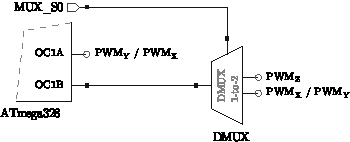
\includegraphics{drive_schem_pwm}
    \end{center}
\end{figure}


\subsection{Διεκπεραίωση}
\label{subsec:motor:autoshut}

Κάθε κινητήρας που χρησιμοποιείται στην υλοποίηση είναι άρρηκτα συνδεδεμένος με
έναν οπτικό κωδικοποιητή περιστροφικής κίνησης (εφεξής, κωδικοποιητής), που
επιτρέπει την παρακολούθηση της κίνησης του. (Οι κωδικοποιητές αναλύονται σε
βάθος στ \nref.)
Ο κωδικοποιητής διαθέτει ένα σήμα εξόδου από το οποίο αποστέλλονται διαδοχικοί
παλμοί για κάθε βήμα του κινητήρα. Καταμετρώντας τους παλμούς είναι δυνατό να
αναχθεί η μετατόπιση που έχει προκληθεί σε κάθε άξονα ώστε, τελικά, να
ακινητοποιηθούν οι κινητήρες, εφόσον η κεφαλή έχει φτάσει στην επιθυμητή θέση.

Σαφώς, η καταμέτρηση είναι δυνατό να πραγματοποιείται από το λογισμικό του
μικροελεγκτή. Ωστόσο, για τους ίδιους λόγους που επιλέγεται παραγωγή σήματος PWM
από το υλικό του μικροελεγκτή και όχι από το λογισμικό, μελετάται το ενδεχόμενο
μίας αντίστοιχης πορείας.


\subsubsection{Μηχανική διεκπεραίωση}

Μία πιθανή λύση παρέχεται από το Χρονομετρητή\slash Απαριθμητή
\textenglish{Timer\slash Counter0}, ο οποίος υποστηρίζει τη χρήση εξωτερικού
ρολογιού για την αύξηση του καταχωρητή\slash μετρητή, TCNT0, σε κάθε εισερχόμενο
παλμό στον ακροδέκτη T0 \parencite[109]{atmel13}. Εφόσον ενεργοποιηθεί μέσω του
καταχωρητή TIMSK0, μόλις η τιμή του TCNT0 γίνει ίση με την τιμή του επιλεγμένου
καταχωρητή σύγκρισης, OCR0x, προκαλείται διακοπή και εκτελείται η αντίστοιχη
ρουτίνα εξυπηρέτησης, γνωστοποιώντας, με αυτόν τον τρόπο, το συμβάν
\parencite[110]{atmel13}. Επομένως, εάν, πριν την ενεργοποίηση κάποιου κινητήρα,
είναι δυνατό να υπολογιστεί το πλήθος το βημάτων που απαιτείται για την μετάβαση
στην επιθυμητή θέση, τότε η τιμή αυτή μπορεί να τεθεί στον OCR0x και, κατόπιν,
να ενεργοποιηθεί ο μετρητής. Έτσι, είναι βέβαιο ότι το λογισμικό θα ειδοποιηθεί
όταν τα βήματα έχουν ολοκληρωθεί.

Ενδέχεται, ωστόσο, τη στιγμή που τίθεται ο ενδείκτης OCF0x του καταχωρητή TIFR0
και που, φυσιολογικά, θα εκτελούταν η αντίστοιχη ρουτίνα εξυπηρέτησης, οι
διακοπές να έχουν απενεργοποιηθεί επειδή βρίσκεται ήδη σε εξέλιξη η εκτέλεση
μίας άλλης ρουτίνας. Σε αυτήν την περίπτωση, μετά την ολοκλήρωση της τρέχουσας
ρουτίνας και την επαναφορά των διακοπών, θα δοθεί στις εν αναμονή διακοπές η
ευκαιρία να εξυπηρετηθούν, πάντα με σειρά προτεραιότητας
\parencite[13--14,57]{atmel13}. Το ενδεχόμενο αυτό θα μπορούσε να προκαλέσει
ανεπιθύμητες παρενέργειες, ιδίως εάν η καθυστέρηση είναι παρατεταμένη. Για
παράδειγμα, η κεφαλή θα συνέχιζε την πορεία της για όσο χρόνο αυτή υφίσταται και
όταν, τελικά, η διακοπή θα εξυπηρετούταν, η κεφαλή θα βρίσκεται σε θέση
διαφορετική από την αναμενόμενη και χωρίς να υπάρχει κάποια σχετική ένδειξη.

Για την αποφυγή τέτοιων καταστάσεων, κρίνεται απαραίτητη η ύπαρξη ενός
μηχανισμού, σε επίπεδο υλικού, που να πυροδοτείται με την ολοκλήρωση των βημάτων
και, με τη σειρά του, να απενεργοποιεί τον κινητήρα. Θα μπορούσε να
αντιπροσωπεύει την αλλαγή της κατάστασης από \emph{off} σε \emph{on}, ενός
διακόπτη που παρεμβάλλεται της πηγής του σήματος PWM και του κινητήρα ώστε να
εμποδίζει την μετάδοση του σήματος.

Η λύση παρέχεται, εν μέρει, από τον ίδιο τον μετρητή με τη δυνατότητά του για
παραγωγή εξόδου στον ακροδέκτη OC0A, όταν ο TCNT0 εξισώνεται με τον OCR0A
\parencite[98--99,107]{atmel13}. Η λειτουργία ονομάζεται CTC (\textenglish{Clear
Timer on Compare Match}) και η παραγόμενη έξοδος επηρεάζεται από τα bit COM0A1:0
του καταχωρητή TCCR0A. Από τις τρεις ρυθμίσεις (\textenglish{Toggle, Clear} και
\textenglish{Set}) επιλέγεται η \textenglish{Toggle} σύμφωνα με την οποία η
έξοδος εναλλάσσεται σε κάθε εξίσωση των TCNT0 και OCR0A. Ωστόσο, αν ο διακόπτης
είναι \textenglish{active hight}, και προκειμένου να τίθεται σε κατάσταση
\textenglish{off} που επιτρέπει τη μετάδοση του σήματος, η τιμή του OC0A πρέπει,
αρχικά, να είναι λογικό 1. Η επιβολή αυτής της τιμής γίνεται με χρήση του bit
FOC0A του καταχωρητή TCCR0B η οποία αλλάζει την έξοδο στον ακροδέκτη OC0A σαν
να είχε προκύψει εξίσωση μεταξύ TCNT0 και OCR0A χωρίς, ωστόσο, να προκαλείται
διακοπή ή επανέναρξη του TCNT0.

Επομένως, τη στιγμή που λαμβάνεται το τελευταίο βήμα από τον κωδικοποιητή, η
έξοδος του OC0A αλλάζει σε λογικό 0 και, έτσι, αποτρέπει την αναμετάδοση του
σήματος PWM (ακροδέκτες OC1A και OC1B), παρότι η γεννήτρια PWM συνεχίζει να
λειτουργεί. Όποτε η CPU του μικροελεγκτή γίνει διαθέσιμη, ενημερώνεται για το
συμβάν (καθώς εκτελείται η σχετική ρουτίνα εξυπηρέτησης) και από εκεί είτε
απενεργοποιείται η γεννήτρια PWM είτε δρομολογείται νέα μετακίνηση.

%
% Things to consider
%

Ο παραπάνω σχεδιασμός, παρότι επιτυγχάνει ένα κρίσιμο χαρακτηριστικό της
υλοποίησης -- τη μηχανική διακοπή τον κινητήρων -- επιβάλλει ορισμένα σημεία
επανεξέτασης. Αρχικά, καθώς ο μετρητής \textenglish{Timer\slash Counter0}
διαθέτει καταχωρητές των 8-bit (δηλαδή, καθένας από τους TCNT0, OCR0A και
OCR0B είναι 8-bit), η μέγιστη τιμή TOP είναι το 255. Αυτό συνεπάγεται ότι
κάθε μεμονωμένη μετακίνηση διαθέτει, το πολύ, 257 βήματα. Εάν απαιτούνται
περισσότερα βήματα, τότε η συνολική μετατόπιση πρέπει να διασπάται σε
μικρότερες μετακινήσεις. (Σημειώνεται ότι τα βήματα είναι, το πολύ, 257 και όχι
256, καθώς 256 παλμοί απαιτούνται για την μετάβαση του TCNT0 από 0 σε 255.
Ωστόσο, η εξίσωση ενεργοποιείται στον επόμενο παλμό -- τον 257 -- ο οποίος και
θέτει τον TCNT0 σε 0.)

Για λόγους πληρότητας, αναφέρεται, επίσης, ότι η συχνότητα των εξωτερικών παλμών
υπόκειται σε έναν βασικό περιορισμό. Σύμφωνα με το εγχειρίδιο της
\textcite[139--140]{atmel13}, η συχνότητα του εξωτερικού ρολογιού πρέπει να
είναι μικρότερη από $f_{clk_{I/O}}/2.5$, ώστε να είναι εγγυημένη η αναγνώριση
όλων των παλμών. Ωστόσο, στην περίπτωσή της υλοποίησης, οι εισερχόμενοι παλμοί
είναι, μόλις, της τάξης των μερικών δεκάδων Hz, ενώ το ρολόι συστήματος, των
μερικών MHz.

Το σημαντικό σημείο προς μελέτη, ωστόσο, είναι το πλήθος των μετρητών βημάτων
που δύνανται να διευθετηθούν. Εφόσον ο \textenglish{Timer\slash Counter1}, ο
οποίος, επίσης, υποστηρίζει συγχρονισμό με εξωτερικό ρολόι, διευθετείται για την
παραγωγή σήματος PWM, απομένει μόνο ο \textenglish{Timer\slash Counter0} για
αυτήν τη λειτουργία και, προφανώς, για έναν μόνο κωδικοποιητή τη φορά. Όπως έχει
αναφερθεί, είναι επιθυμητή η ταυτόχρονη κίνηση στους άξονες X και Y, όποτε αυτό
απαιτείται.


\subsubsection{Μέγιστη κοινή μετατόπιση}
\label{ssubsec:motor:common-translation}

\begin{figure}
    \caption{Αλληλουχία κύκλων μετατόπισης.\label{fig:motor:translation}}
    \begin{center}
    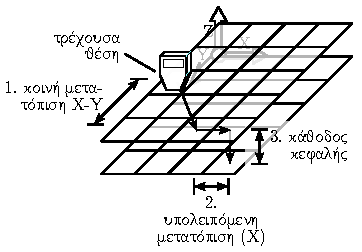
\includegraphics{drive_translation}
    \end{center}
\end{figure}

Κρίνεται αναγκαίος και ικανός ο ακόλουθος ανασχεδιασμός. Ο ακροδέκτης T0
λαμβάνει το βήμα ενός εκ των τριών κωδικοποιητών κίνησης, με την επιλογή κάποιου
να γίνεται μέσω πολυπλέκτη. Στην περίπτωση όπου απαιτείται κίνηση και στους δύο
άξονες X και Y, ο \textenglish{Timer\slash Counter0} διευθετείται ώστε να
καταμετράει τα βήματα ενός εκ των δύο. Οι δύο κινητήρες δρομολογούνται για τη
μέγιστη κοινή, κατά μέτρο, μετατόπιση. Με την ολοκλήρωση του πρώτου κύκλου
βημάτων, η πλήρης μετατόπιση τουλάχιστον του ενός εκ των δύο αξόνων θα έχει
καλυφθεί. Εφόσον εκκρεμεί μετατόπιση για τον άλλο, ξεκινάει ένας δεύτερος κύκλος
για τα υπολειπόμενα βήματα. Η αλληλουχία των κύκλων μετατόπισης πασουριάζεται
στο σχήμα \ref{fig:motor:translation}.

Αυτός ο σχεδιασμός επιβάλλει, ωστόσο, οι κινητήρες X και Y, να λειτουργούν με
την ίδια γωνιακή ταχύτητα, ώστε στο χρόνο που απαιτεί ο ένας να περιστραφεί
ένα συγκεκριμένο αριθμό βημάτων, να ολοκληρώνει και ο άλλος τον ίδιο αριθμό
βημάτων. Στην υλοποίηση, και κατόπιν αρκετών αναπροσαρμογών του κύκλου εργασίας
των κινητήρων, η συμπεριφορά αυτή προσεγγίζεται σε βαθμό που παράγει, σχετικά,
ικανοποιητικά αποτελέσματα.

Στο σχήμα \ref{fig:motor:route_steps} εμφανίζεται η ανασχεδιασμένη παραδοχή
όπου διακόπτες ελεγχόμενοι από την έξοδο του μετρητή βημάτων παρεμβάλλονται των
γραμμών του σήματος PWM, ενώ ο αποπολυπλέκτης 2 τροφοδοτεί το μετρητή με βήματα
ενός εκ των τριών κωδικοποιητών. Ο αποπολυπλέκτης 1-προς-2 του προηγούμενου
σχεδιασμού έχει αντικατασταθεί από δύο διακόπτες οι οποίοι παρέχουν ισοδύναμα
αποτελέσματα, δεδομένου ότι οι κωδικοποιητές συνδέονται στα τρία πρώτα κανάλια
του αποπολυπλέκτη και ότι η παραγωγή σήματος PWM είναι απενεργοποιημένη όταν η
λογική τιμή των MUX\tsub{S1:0} είναι 0x3. Η δεύτερη προϋπόθεση είναι αυτονόητη
καθώς θεωρείται μη έγκυρη κατάσταση η προώθηση σήματος σε κινητήρα, χωρίς την
ενεργοποίηση του αντίστοιχου κωδικοποιητή.

Η χρήση διακοπτών αντί του 1-προς-2 πολυπλέκτη έχει το επιπρόσθετο πλεονέκτημα
ότι μαζί με τους άλλους δύο διακόπτες σχηματίζεται ένα τετραμερές ολοκληρωμένο
κύκλωμα διακοπτών όπως, για παράδειγμα, το CD4016.

Επίσης, έχει εισαχθεί ένας ακόμα αποπολυπλέκτης ο οποίος θέτει σε λειτουργία
τον αντίστοιχο κωδικοποιητή, ουσιαστικά, ενεργοποιώντας τη δίοδο υπερύθρων που
διαθέτει. Για λόγους που έχουν αναφερθεί σε προηγούμενο κεφάλαιο, όπως η
επιμήκυνση της διάρκειας ζωής της διόδου καθώς και η μείωση της κατανάλωσης
ισχύος, ο κάθε κωδικοποιητής ενεργοποιείται μόνο για το χρονικό διάστημα που
περιστρέφεται ο αντίστοιχος κινητήρας.

\begin{figure}
    \caption{Λογική σύνδεση μετρητή βημάτων και κινητήρων.
    \label{fig:motor:route_steps}}
    \begin{center}
    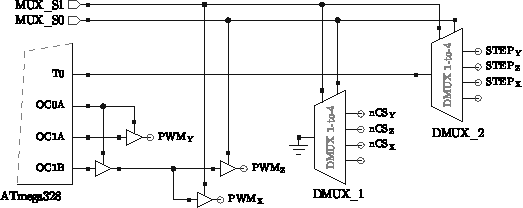
\includegraphics{drive_schem_step-and-pwm}
    \end{center}
\end{figure}

Τα εναπομείναντα κανάλια των δύο αποπολυπλεκτών μπορούν να χρησιμοποιηθούν για
την κάλυψη άλλων αναγκών, δεδομένου ότι η χρήση γίνεται όταν το υποσύστημα
κινητήρων βρίσκεται σε αδράνεια. Για παράδειγμα, το τέταρτο κανάλι του MUX\_1
μπορεί να συνδεθεί με τον ακροδέκτη \nbar{CS} κάποιου άλλου ολοκληρωμένου, ενώ
του MUX\_2, για την ανταλλαγή δεδομένων όταν ο μετρητής βημάτων είναι
απενεργοποιημένος.

\section{Εγκλωβισμός και επανάκαμψη}
\label{sec:motor:backtrack}

Η ύπαρξη των κωδικοποιητών κίνησης αιτιολογείται από την ανάγκη ανατροφοδότησης
σχετικά με την πορεία εξέλιξης της μετατόπισης σε κάθε άξονα. Ωστόσο, οι
κωδικοποιητές, αυτοσχέδιοι ή μη, είναι, έως ένα βαθμό, επιρρεπείς σε εσφαλμένες
μετρήσεις, κάτι που καθορίζεται από τη διακριτική τους ικανότητα
\parencite[15--16]{albert11}. Επιπλέον, η υπόθεση ότι, κατά τη μέγιστη κοινή
μετατόπιση, ο αριθμός βημάτων που πραγματοποιείται σε κάθε άξονα είναι ο ίδιος
και για τους δύο, εισάγει επιπρόσθετη πιθανότητα αστοχίας. Ανεξαρτήτως της
συχνότητας εμφάνισης, κρίνεται απαραίτητη η ύπαρξη ενός μηχανισμού ως έσχατη
προστασία κατά της εξώθησης της κεφαλής πέραν των φυσικών ορίων (του πλαισίου)
της συσκευής που οφείλεται σε αδυναμία αναγνώρισης ή παρακολούθησης της
πραγματικής θέσης της κεφαλής.

% nref: Χρήση διακοπτών στην Κατασκευή
Η λύση περιλαμβάνει τη στερέωση μηχανικών διακοπτών σε κάθε πλευρά των κινητών
μερών της συσκευής ώστε κατά την πρόσκρουσή τους με τα άκρα του πλαισίου, αφενός
να απενεργοποιούνται οι κινητήρες και, αφετέρου, να ειδοποιείται ο μικροελεγκτής
για το συμβάν. Και σε αυτήν την περίπτωση, θεωρείται ζωτικής σημασίας η
απενεργοποίηση να συμβαίνει σε επίπεδο υλικού, ενώ το λογισμικό να επεμβαίνει
στην πορεία, όταν ευκαιρήσει. Το σχήμα \ref{fig:motor:limit-switch} παρουσιάζει
τη βασική ιδέα.

\begin{figure}
    \caption{Συνδεσμολογία εγκλωβισμού και επανάκαμψης κινητήρα σε ένα άκρο.
    \label{fig:motor:limit-switch}}
    \begin{center}
    
\includegraphics{drive_schem_limit-and-bck}
    \end{center}
\end{figure}

Ο επιλεγμένος διακόπτης είναι SPDT (\textenglish{Single Pole, Double Throw})
και, συνεπώς, διαθέτει τρεις ακροδέκτες· όταν ο διακόπτης είναι ελεύθερος, ο
ακροδέκτης NC (\textenglish{Normally Closed}) συνδέεται με τον COM
(\textenglish{Common}), ενώ όσο βρίσκεται πιεσμένος, ο ακροδέκτης NO
(\textenglish{Normally Open}) συνδέεται με τον COM, ενώ ο NC είναι
αποσυνδεδεμένος. Η τοποθέτηση του διακόπτη στη γραμμή τροφοδοσίας του κινητήρα
επιτρέπει τη μηχανική αποσύνδεσή του όποτε ο διακόπτης πιέζεται.

Προκειμένου να ειδοποιείται ο μικροελεγκτής ότι ο κινητήρας έχει ακινητοποιηθεί,
θα πρέπει η αλλαγή της κατάστασης του διακόπτη να προκαλεί εναλλαγή σε κάποιο
εισερχόμενό του σήμα. Δεδομένου ότι η σύνδεση του ακροδέκτη NO με τον COM θέτει
το σήμα αυτό σε λογικό 0, το σήμα θα πρέπει, υπό φυσιολογικές συνθήκες, να
βρίσκεται σε λογικό 1. Αυτό αιτιολογεί την ύπαρξη αντιστάτη pull-up στο
σχήμα \ref{fig:motor:limit-switch}, ώστε η γραμμή LIMIT να τίθεται σε λογικό 1,
από προεπιλογή. Από πλευράς ρυθμίσεων, ο μικροελεγκτής αρκεί να διευθετηθεί ώστε
να προκαλείται διακοπή στην εναλλαγή του σήματος του συνδεδεμένου ακροδέκτη
(\textenglish{level triggered} ή \textenglish{edge triggered}). Οι λεπτομέρειες
αναλύονται στην \nameref{subsec:motor:limit-pin-change} (σ.~%
\pageref{subsec:motor:limit-pin-change}).

Η αναγνώριση του συμβάντος από το μικροελεγκτή είναι απαραίτητη ώστε ο κινητήρας
να τίθεται σε κατάλληλη θέση για τη συνέχιση της λειτουργίας του. Αφενός
απαιτείται η αλλαγή του κύκλου εργασίας του σήματος PWM ώστε ο κινητήρας να
περιστρέφεται με φορά αντίθετη αυτής που προκάλεσε τη διακοπή για χρονικό
διάστημα μέχρι την απελευθέρωση του διακόπτη.
Ωστόσο, η αλλαγή
του κύκλου εργασίας από μόνη της είναι αδύνατο να επαναφέρει τον κινητήρα καθώς
αυτός είναι μηχανικά αποσυνδεδεμένος από την τροφοδοσία (εξαιτίας του πιεσμένου
διακόπτη).
Για το λόγο αυτό, παρέχεται ένας ηλεκτρονικός διακόπτης ως εφεδρική σύνδεση με
την τάση αναφοράς (GND). Όταν ο κινητήρας έχει οπισθοδρομήσει αρκετά ώστε να
απεγκλωβιστεί από τον μηχανικό διακόπτη, ο ηλεκτρονικός διακόπτης
απενεργοποιείται και ο κινητήρας είναι σε θέση να λειτουργηθεί κανονικά.

Στο σχήμα απεικονίζεται, επίσης, μία δίοδος επιστροφής συνδεδεμένη στα άκρα του
κινητήρα. Ο λόγος ύπαρξής της είναι η εξομάλυνση παλμών που δημιουργούνται κατά
την κατάρρευση του μαγνητικού πεδίου του πηνίου του κινητήρα όταν αυτός
αποσυνδέεται από την τροφοδοσία \parencite[130--132]{kuphaldt09semi}. Ωστόσο,
κρίνεται ότι στην περίπτωση της υλοποίησης, η οποία χρησιμοποιεί σερβοκινητήρες,
η ανάγκη για τη συμπερίληψή τους είναι μικρή και, τελικά, αποκλείονται από
αυτήν.

\subsection{Προσαρμογή στις ανάγκες της υλοποίησης}

Η προαναφερθείσα συνδεσμολογία αγνοεί το γεγονός ότι απαιτούνται δύο
ανασταλτικοί διακόπτες SPDT ανά κινητήρα -- έναν για κάθε άκρο -- καθώς και το
γεγονός ότι ο κινητήρας Z κινείται μόνο εφόσον οι άλλοι δύο βρίσκονται σε
ηρεμία. Το τελευταίο θα μπορούσε να χρησιμοποιηθεί για τη μείωση του αριθμού των
παραγόμενων σημάτων. Στο σχήμα \ref{fig:motor:limit-switch_final} παρουσιάζεται
η τελική συνδεσμολογία. Παρατηρείται ότι οι ανασταλτικοί διακόπτες των αξόνων X
και Z συνδέονται σε σειρά και ότι χρησιμοποιείται μόνο ένας ηλεκτρονικός
διακόπτης για την εφεδρική σύνδεση με την τάση αναφοράς (BCK\tsub{XZ}).
Αντιστοίχως, δεσμεύεται μόνο ένας ακροδέκτης του μικροελεγκτή για την ειδοποίηση
εγκλωβισμού κάποιου εκ των δύο κινητήρων (LIMIT\tsub{XZ}).

\begin{figure}
    \caption{Πλήρης συνδεσμολογία εγκλωβισμού και επανάκαμψης.
    \label{fig:motor:limit-switch_final}}
    \begin{center}
    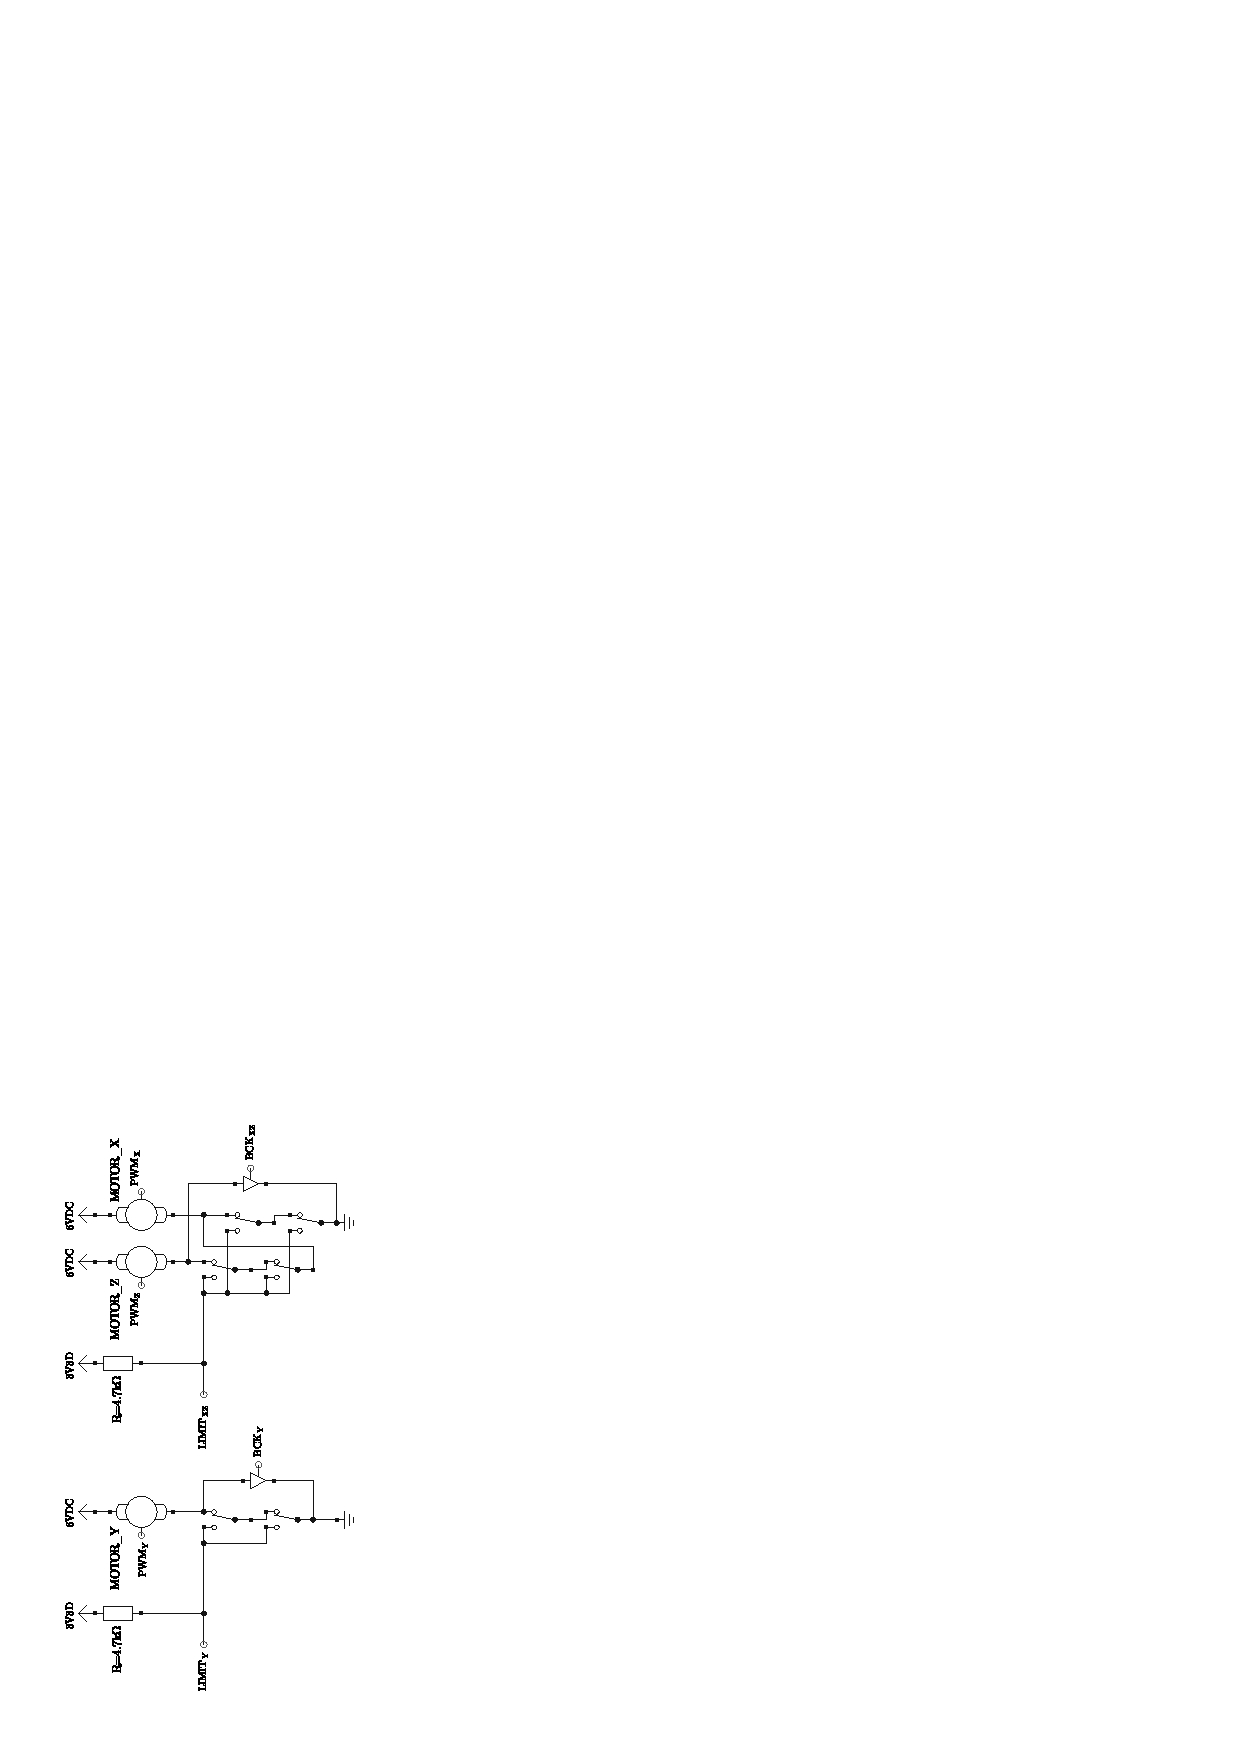
\includegraphics{drive_schem_limit-and-bck_all}
    \end{center}
\end{figure}

Ο λόγος για τη συγχώνευση των κυκλωμάτων των κινητήρων X και Z αντί των Y και Z
είναι η διευκόλυνση της φυσικής διασύνδεσης των διακοπτών λόγω της εγγύτητας των
δύο αξόνων.
% nref: Διάταξη αξόνων (Z over X).
Η σύνδεση X και Y, σαφώς, απορρίπτεται, καθώς αυτοί οι δύο κινητήρες δύνανται να
τεθούν σε λειτουργία ταυτόχρονα και θα ήταν, συνεπώς, αδύνατο να εντοπιστεί
ποιος από τους δύο έχει εγκλωβιστεί.

Το βασικό μειονέκτημα της επιλεγμένης μεθόδου είναι ότι επιτρέπει την αναγνώριση
του κυκλώματος κινητήρων και όχι του συγκεκριμένου διακόπτη που προκαλεί τον
εγκλωβισμό. Συνεπώς, εφόσον οι κινητήρες τίθενται σε κίνηση από το μικροελεγκτή
και στην πορεία προκύπτει εγκλωβισμός, η κατάσταση είναι δυνατό να αναστραφεί.
Ωστόσο, αν κατά την εκκίνηση της συσκευής κάποιος κινητήρας είναι εγκλωβισμένος,
αυτός ο μηχανισμός από μόνος του είναι ανεπαρκής για την επανάκαμψή του. Η
παρούσα υλοποίηση αρκείται σε αυτόν το μηχανισμό χωρίς να καταβάλει προσπάθεια
επανάκαμψης στην προαναφερθείσα περίπτωση.

\subsection{Αναγγελία εγκλωβισμού}
\label{subsec:motor:limit-pin-change}

Αναφέρθηκε προηγουμένως η ανάγκη διευθέτησης του μικροελεγκτή για την απόκριση
του στην εναλλαγή των σημάτων LIMIT\tsub{XZ} και LIMIT\tsub{Y}. Σύμφωνα με το
εγχειρίδιο του μικροελεγκτή της \textcite[71]{atmel13}, εξωτερικές διακοπές
είναι δυνατό να ενεργοποιηθούν για εισερχόμενες παρυφές (\textenglish{edge
triggered}) σε οποιοδήποτε ακροδέκτη PCINT ή, επιπροσθέτως, για οποιαδήποτε
λογική αλλαγή στους ακροδέκτες INT0 και INT1. Προτιμάται η χρήση δύο PCINT
ακροδεκτών καθώς καλύπτουν τις απαιτήσεις ενώ, ταυτόχρονα, επιτρέπουν τη χρήση
των ειδικών ακροδεκτών INT0 και INT1 σε περιπτώσεις όπου διακοπή σε εναλλαγή
σήματος είναι ακατάλληλη.

Το σύνολο των ακροδεκτών PCINT διαμοιράζεται σε τρεις ομάδες. Η εναλλαγή του
σήματος ενός οποιουδήποτε ακροδέκτη κάθε ομάδας προκαλεί την εκτέλεση της ίδιας
ρουτίνας εξυπηρέτησης, εφόσον το bit της αντίστοιχης ομάδας του καταχωρητή PCICR
(\textenglish{Pin Change Interrupt Conrol Register}) έχει τεθεί. Επιπλέον, με
τους καταχωρητές PCMSK (\textenglish{Pin Change Mask Register}) -- 1, 2 και 3 --
προσδιορίζονται ποιοι PCINT ακροδέκτες κάθε ομάδας είναι επιθυμητό να προκαλούν
διακοπή.

Το γεγονός ότι όλοι οι ακροδέκτες του μικροελεγκτή αντιστοιχίζονται με κάποιον
PCINT, καθιστούν εύκολη την επιλογή και ανάθεση δύο εξ αυτών στα σήματα
LIMIT\tsub{XZ} και LIMIT\tsub{Υ}. Ωστόσο, προτιμώνται δύο ακροδέκτες PCINT που
ανήκουν στην ίδια ομάδα με αποτέλεσμα να καλείται η ίδια ρουτίνα εξυπηρέτησης
ώστε η αναγνώριση του εγκλωβισμένου κινητήρα να επαφίεται στο ίδιο το λογισμικό
(σαφώς με τη βοήθεια των σημάτων).

\section{Παλιννόστηση}
\label{sec:motor:homing}

Κατά την ενεργοποίηση της συσκευής (σύνδεση με τροφοδοσία) καθώς και κατά τον
εγκλωβισμό και επανάκαμψη κάποιου κινητήρα, κρίνεται απαραίτητη η επαναφορά της
κεφαλής σε μία γνωστή θέση, τη θέση επιστροφής (\textenglish{machine home})
\parencite[99]{albert11}. Από εκείνο το σημείο, είναι δυνατόν η κεφαλή να
δρομολογηθεί σε νέα θέση ή και σε αυτήν που προκάλεσε τον εγκλωβισμό.

Κατά βάση, ο μηχανισμός είναι ίδιος και στις δύο περιπτώσεις. Αρχικά, ο
κινητήρας Z διευθετείται για την πραγματοποίηση του μέγιστου δυνατού -- και όχι
το μέγιστου αποδεκτού -- πλήθους βημάτων με διεύθυνση που οδηγεί την κεφαλή στη
θέση επιστροφής για αυτόν τον άξονα. Εν τέλει, προκαλείται, νέος εγκλωβισμός
κινητήρα. Και σε αυτήν την περίπτωση, ο μηχανισμός επανάκαμψης αναλαμβάνει,
αυτόματα, την οπισθοδρόμηση της κεφαλής έως ότου απεγκλωβιστεί ο κινητήρας.
Ωστόσο, με την ολοκλήρωση της επανάκαμψης, είναι γνωστό ότι η κεφαλή βρίσκεται
στη θέση επιστροφής για τον άξονα Z. Σε δεύτερο στάδιο, εφαρμόζεται η ίδια
διαδικασία, αυτήν τη φορά, για τους άξονες X και Υ, ταυτόχρονα. Με την
επανάκαμψη και των δύο, η κεφαλή θεωρείται ότι βρίσκεται στη θέση επιστροφής.

Αναφέρθηκε, προηγουμένως, η δυνατότητα της συσκευής για την εκ νέου δρομολόγηση
της κεφαλής σε περίπτωση κατά την οποία η προηγούμενη διακόπτεται απρόοπτα από
εγκλωβισμό κινητήρα. Ο λόγος είναι ότι το συμβάν του εγκλωβισμού μπορεί να
οφείλεται σε αστοχία παρακολούθησης της θέσης της κεφαλής. Σε αυτήν την
περίπτωση, και εφόσον η κεφαλή έχει μόλις αρχικοποιηθεί, ενδέχεται η νέα
προσπάθεια να επιφέρει τα επιθυμητά αποτελέσματα. Η υπόθεση βασίζεται στην
παραδοχή ότι κάθε μετακίνηση εισάγει ένα ποσοστό απόκλισης μεταξύ αναγνωρισμένης
και πραγματικής θέση της κεφαλής. Επομένως, πολλαπλές μετακινήσεις ενδέχεται
να προκαλέσουν μεγαλύτερη συνολική απόκλιση. Κατόπιν ολοκλήρωσης της
παλιννόστησης, η συσκευή διαθέτει μία πρόσφατη και έγκυρη αναγνώριση θέσης.

Ωστόσο, σε περίπτωση που η επιθυμητή θέση είναι, στην πραγματικότητα,
απροσπέλαστη, για παράδειγμα, εξαιτίας κάποιου παρεμβαλλόμενου εμποδίου, η
παραπάνω συμπεριφορά προκαλεί έναν ατέρμονα βρόχο παλιννόστησης και
(επανα)δρομολόγησης. Η κατάσταση αυτή, προφανώς ανεπιθύμητη, αποφεύγεται
αποτρέποντας τη δρομολόγηση της ίδιας θέσης εφόσον, τη στιγμή του εγκλωβισμού,
υπάρχει ένδειξη ότι είναι η πρώτη μετακίνηση μετά από παλιννόστηση.


%W5100

Η χρήση του ολοκληρωμένου επιλέγεται να γίνει δια μέσω της πλακέτας WIZ811MJ της
ίδιας εταιρείας. Οι λόγοι είναι ότι επιλύει τη διασύνδεση του ολοκληρωμένου με
συνδετήρα RJ-45 (απαραίτητος για την ανταλλαγή δεδομένων μεταξύ W5100 και
δικτύου), ταλαντωτή και διάφορα άλλα ηλεκτρονικά στοιχεία. Από τους 80,
συνολικά, ακροδέκτες του W5100, το WIZ811MJ διαθέτει μόλις 40, οι οποίοι είναι
αυτοί που προορίζονται για τη διασύνδεση με μικροελεγκτή. Όλοι οι υπόλοιποι
συμμετέχουν σε εσωτερικές συνδέσεις της πλακέτας.

Ένα παράδειγμα σχετικά με το τελευταίο, το W5100 διαθέτει έναν ακροδέκτη για το
χειρισμό του ολοκληρωμένου ως Slave σε δίαυλο SPI, το \nbar{SCS}
(\textenglish{SPI Chip-Select}) \parencite[9]{wiz11:w5100}. Ωστόσο, διαθέτει και
έναν επιπρόσθετο ακροδέκτη, τον SEN (\textenglish{SPI Enable}), για την
ενεργοποίηση των υποσυστημάτων του ολοκληρωμένου για λειτουργία σε SPI
\parencite[8]{wiz11:w5100}. Το WIZ811MJ παρέχει ακροδέκτη μόνο για το \nbar{SCS}
ενώ διαθέτει κατάλληλη διάταξη ώστε η αλλαγή της τιμής του να προκαλεί το
αναμενόμενο σήμα στο SEN, αυτομάτως \parencite[7]{wiz13:811mj}.

Επιπλέον σημαντικό χαρακτηριστικό είναι ότι η πλακέτα παρέχει ακροδέκτες
συμβατούς με πρωτότυπες κάρτες (\textenglish{breadboard}) που χρησιμοποιεί η
υλοποίηση, εν αντιθέσει με το W5100 το οποίο είναι SMD
(\textenglish{Surface-Mount Device}) και απαιτεί συγκόλληση
\parencite[6,12]{wiz13:811mj}.

%Αποτελεί μία έτοιμη λύση για την προσθήκη δικτυακών δυνατοτήτων στην υλοποίηση.
%W5100 + MAG-JACK


\subsection{Επικοινωνία με μικροελεγκτή}

Το W5100 υποστηρίζει τρεις τρόπους για την επικοινωνία με το μικροελεγκτή· άμεση
ή έμμεση προσπέλαση ή, μέσω πρωτοκόλλου SPI \parencite[59]{wiz11:w5100}. Οι δύο
πρώτες μέθοδοι χρησιμοποιούν διαύλους διεύθυνσης και δεδομένων απαιτώντας πολλά
σημεία σύνδεσης με το μικροελεγκτή· για την ακρίβεια, 3 γραμμές ελέγχου
(\textenglish{Chip-Select, Read, Write}), 8 γραμμές για το δίαυλο δεδομένων,
και, 15 ή 2 γραμμές διεύθυνσης για άμεση ή έμμεση προσπέλαση, αντίστοιχα. Στην
περίπτωση του SPI απαιτούνται πολύ λιγότερες (μόλις 4) και αυτός είναι ο λόγος
που προτιμάται για τη διασύνδεση του με την MCU, δεδομένου του περιορισμένου
αριθμού ακροδεκτών της. Σαφώς, το μειονέκτημα χρήσης SPI -- ενός σειριακού
πρωτοκόλλου επικοινωνίας -- είναι ότι επιτυγχάνεται πολύ μικρότερος ρυθμός
ανταλλαγής δεδομένων από ότι στην περίπτωση των άλλων δύο, κάτι που, τελικά,
επηρεάζει το χρόνο απόκρισης στα εισερχόμενα αιτήματα. Ωστόσο, κρίνεται ότι για
τις ανάγκες της υλοποίησης, αυτός ο περιορισμός είναι αμελητέος σε σχέση με την
εξοικονόμηση ακροδεκτών που επιφέρει η χρήση SPI.

\begin{figure}
    \caption{Πλακέτα WIZ811MJ και διάταξη των ακροδεκτών του W5100.
    \label{fig:net:811mj-pins}}
    \begin{center}
    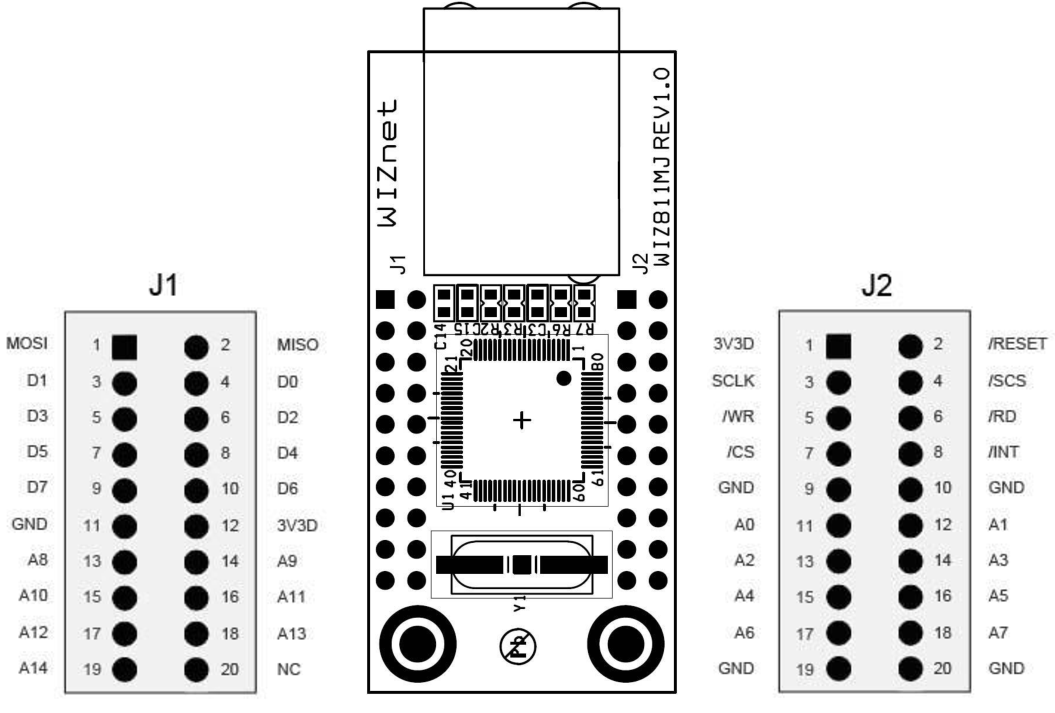
\includegraphics[width=0.9\textwidth]{network_811mj_pin-layout}
    \end{center}
    \fullcite[6]{wiz13:811mj:pins}
\end{figure}

% συνδεσμολογία
Το σχήμα \ref{fig:net:811mj-pins} παρουσιάζει την πλακέτα WIZ811MJ και, σε
μεγέθυνση, την ονομασία των ακροδεκτών της. Από τους ακροδέκτες J1, ιδιαίτερου
ενδιαφέροντος είναι οι 1 (MOSI), 2 (MISO) και 12 (3V3D) εκ των οποίων οι δύο
πρώτοι χρησιμοποιούνται για την μετάδοση των bit του \textenglish{Master} και
του ενεργού \textenglish{Slave} του διαύλου SPI, αντίστοιχα, ενώ ο τελευταίος,
για την τροφοδοσία της πλακέτας με τάση 3.3V. Οι υπόλοιποι, με εξαίρεση τον 20
(\textenglish{Not Connected}), συνδέονται με την τάση αναφοράς, δεδομένου ότι
όλοι, με εξαίρεση τον ακροδέκτη 11 (GND), χρησιμοποιούνται μόνο στην περίπτωση
άμεσης ή έμμεσης προσπέλασης.

Από τους ακροδέκτες J2, ο 1 (3V3D) χρησιμοποιείται για τροφοδοσία 3.3V ενώ οι
9, 10, 19 και 20 (GND) συνδέονται με την τάση αναφοράς. Οι 3 (SCLK) και
(\nbar{SCS}) αποτελούν μέρος του διαύλου SPI για τη μεταφορά του ρολογιού από
το \textenglish{Master} και την ενεργοποίηση του W5100 ως \textenglish{Slave}.
Σύμφωνα με το εγχειρίδιο της \textcite[8]{wiz13:811mj}, ο ακροδέκτης 2
(\nbar{RESET}) προκαλεί την αρχικοποίηση όλων των καταχωρητών του W5100 στις
προεπιλεγμένες τους τιμές και κρίνεται ότι αρκεί να συνδεθεί με το αντίστοιχο
σήμα του μικροελεγκτή ώστε η αρχικοποίηση του W5100 να πραγματοποιείται μαζί
με το μικροελεγκτή.

Οι ακροδέκτες 5 (\nbar{WR}), 6 (\nbar{RD}) και 7 (\nbar{CS}) χρησιμοποιούνται
στην περίπτωση επικοινωνίας μέσω άμεσης ή έμμεσης προσπέλασης και όχι σε SPI
\parencite[8]{wiz11:w5100}. Ωστόσο, επειδή είναι \textenglish{active low},
τίθενται σε μόνιμο λογικό 1 (3.3V), μέσω αντιστάτη, ώστε να είναι λογικά
ανενεργοί.

Μέσω του ακροδέκτη 8 (\nbar{INT}), και εφόσον έχει διευθετηθεί ακολούθως, το
W5100 αναγγέλλει την επιθυμία του για επικοινωνία με το μικροελεγκτή (για
παράδειγμα, επειδή έχουν καταφθάσει δεδομένα). Σε αντίθετη περίπτωση, ο
μικροελεγκτής είναι υποχρεωμένος να εξετάζει από μόνος του το ενδεχόμενο για
επικοινωνία (\textenglish{polling}). Για την υλοποίηση, κρίνεται αξιόλογη η
χρήση των διακοπών. Περισσότερες λεπτομέρειες παρέχονται στην
\nameref{ssubsec:network:ir_imr}.

Για λόγους που έχουν αναφερθεί, όλοι οι υπόλοιποι ακροδέκτες συνδέονται με την
τάση αναφοράς.

Στο σχήμα \ref{fig:network:spi_reset_int} εμφανίζεται η συνδεσμολογία του
μικροελεγκτή με τους ακροδέκτες του W5100 (δια μέσω της πλακέτα WIZ811MJ).
Αξίζει να σημειωθεί ότι, παρόλο που το W5100 λειτουργεί με τάση έως και 3.6V,
ανέχεται τάση στα σήματα εισόδου έως και 5.5V (\textenglish{5V tolerant})
\parencite[64]{wiz11:w5100}. Το χαρακτηριστικό αυτό είναι ιδιαίτερα σημαντικό
επειδή καθιστά δυνατή τη διασύνδεσή του με το μικροελεγκτή χωρίς να απαιτούνται
επιπρόσθετα ενδιάμεσα κυκλώματα για λογικό μετασχηματισμό. %\nref{}

\begin{figure}
    \caption{Διασύνδεση μικροελεγκτή και W5100.
    \label{fig:network:spi_reset_int}}
    \begin{center}
    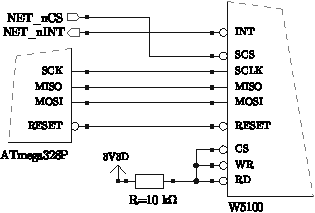
\includegraphics{network_schem_spi_reset_int}
    \end{center}
\end{figure}


\subsection{Διευθέτηση W5100}

Οι καταχωρητές του W5100 χωρίζονται σε δύο κύριες ομάδες· τους καταχωρητές
γενικών ρυθμίσεων (ή κοινοί καταχωρητές) και τους καταχωρητές Socket. Οι κοινοί
καταχωρητές επηρεάζουν τη συμπεριφορά του W5100 συνολικά ή προσδιορίζουν κάποια
χαρακτηριστικά όλων των Socket, ενώ οι καταχωρητές Socket είναι υπεύθυνοι για
τη λειτουργία καθενός εκ των τεσσάρων Socket του ολοκληρωμένου.

Όλοι οι καταχωρητές αντιστοιχίζονται μία διεύθυνση, ενώ υπάρχουν καταχωρητές
περισσοτέρων του ενός byte. Η πρόσβαση σε αυτούς τους καταχωρητές, είτε
πρόκειται για ανάγνωση είτε για εγγραφή, γίνεται από τη χαμηλότερη προς την
υψηλότερη διεύθυνση με \te{Big Endian} διάταξη των byte
\parencite[32--33,35]{wiz11:w5100}.

Οι κοινοί καταχωρητές τίθενται μόνο μία φορά, κατά την εκκίνηση της συσκευής,
και, οι ορισμένοι, κατόπιν εισερχόμενων αιτημάτων (για παράδειγμα, αλλαγή
διεύθυνσης IP). Σε αντίθεση, η πρόσβαση στους καταχωρητές Socket, οι οποίοι
χρησιμοποιούνται για το χειρισμό κάθε Socket, είναι πιο συχνή.


\subsubsection{Καταχωρητές διευθύνσεων και μάσκας υποδικτύου}
\label{ssubsec:network:addr-registers}

Σε αυτήν την κατηγορία συγκαταλέγονται καταχωρητές που ρυθμίζουν τη διεπαφή για
τη σύνδεση με το δίκτυο μέσω των GAR (\te{Gateway Address Register}),
SUBR (\te{Subnet Mask Register}), SHAR (\te{Source Hardware Address Register})
και SIPR (\te{Source IP Address Register}) \parencite[20]{wiz11:w5100}. Η αλλαγή
της τιμής κάποιου, έχει άμεση εφαρμογή στη διεπαφή, γεγονός που λαμβάνεται υπόψη
σε σχετικά εισερχόμενα αιτήματα ώστε να δίνεται απόκριση με τις τρέχουσες
ρυθμίσεις της διεπαφής πριν την ενημέρωσή τους.
% \nref: stored in back-up memory.


\subsubsection{Μέγεθος μνήμης ανά Socket}
\label{ssubsec:network:rmsr_tmsr}

Το W5100 υποστηρίζει μέχρι τέσσερα, ταυτόχρονα, ενεργά Socket καθένα από τα
οποία αποδίδεται ένα μέρος μνήμης από τα συνολικά διαθέσιμα 8KiB για κάθε
κατεύθυνση κίνησης δεδομένων, ανεξάρτητου μεγέθους το καθένα. Οι καταχωρητές
RMSR (\te{RX Memory Size Register}) και TMSR (\te{TX Memory Size Register})
καθορίζουν την προσωρινή μνήμη που αφιερώνεται σε κάθε Socket μεταξύ 1, 2, 4 ή 8
KiB. Σαφώς, πρέπει να δίνεται προσοχή ώστε ο ανατεθειμένος χώρος στα Socket
να μην ξεπερνάει τα 8KiB καθώς, σε αυτήν την περίπτωση, ορισμένα Socket θα
εργάζονται σε κοινές θέσεις στη μνήμη, με ότι επακόλουθα μπορεί αυτό να
επιφέρει.

\begin{figure}
    \caption{Καταχωρητές μεγέθους, RMSR και TMSR.\label{fig:network:rmsr_tmsr}}
    \begin{center}\begin{tabu} spread 0pt {|*8{X[-1,c]|}}

    \hline\rowfont\bfseries
    \multicolumn2{|c}{Socket 3}     &
    \multicolumn2{|c}{Socket 2}     &
    \multicolumn2{|c}{Socket 1}     &
    \multicolumn2{|c|}{Socket 0}   \\

    \hline

    S1  &  S0  &  S1  &  S0  &  S1  &  S0  &  S1  &  S0                       \\
    \hline
    \end{tabu}\end{center}

    Το μέγεθος κάθε Socket καθορίζεται από την τιμή $2^{\text{S1:0}}$.
\end{figure}

Το σχήμα \ref{fig:network:rmsr_tmsr} παρουσιάζει τη σημασιολογία των bit των
δύο αυτών καταχωρητών. Παρατηρείται ότι το μέγεθος της μνήμης κάθε Socket
ρυθμίζεται από δύο, μόνο, bit.
Η υλοποίηση χρησιμοποιεί μόνο ένα Socket με σκοπό τη λήψη και απόκριση αιτημάτων
HTTP. Για το λόγο αυτό οι RMSR και TMSR ρυθμίζονται ώστε να αποδίδονται 8KiB
τόσο για την εισερχόμενη όσο και για την εξερχόμενη προσωρινή μνήμη αποθήκευσης
του Socket 0. Οι ρυθμίσεις του Socket ολοκληρώνονται στην παράγραφο
\nameref{ssubsec:network:port_mr} (σ. \pageref{ssubsec:network:port_mr}).


\subsubsection{Κατάσταση και διακοπές}
\label{ssubsec:network:ir_imr}

Δύο τελευταίοι καταχωρητές που εξετάζονται είναι οι IR(\te{Interrupt Register})
και IMR (\te{Interrupt Mask Register}), οι οποίοι καθορίζουν την κατάσταση
του W5100 και την αναγγελία διακοπών, αντιστοίχως· τα bit του καταχωρητή IR --
μόνο για ανάγνωση -- τίθενται σε κάθε περίπτωση που το απαιτεί, ενώ διακοπή
(μέσω του ακροδέκτη \nbar{INT}) προκαλείται μόνο όταν τίθενται bit του IR των
οποίων το αντίστοιχο bit του IMR έχει, επίσης, τεθεί
\parencite[21--22]{wiz11:w5100}. Με αυτόν τον τρόπο, αναγγέλλονται μόνο οι
διακοπές που ενδιαφέρουν. Επιπλέον, ο μικροελεγκτής εξετάζοντας τον IR μπορεί,
ανά πάσα στιγμή, να αποφασίσει εάν το W5100 χρειάζεται την προσοχή του.

Τα bit των καταχωρητών IR και IMR παρουσιάζονται στο σχήμα
\ref{fig:network:ir_imr}. Από τα συνολικά 7 διαθέσιμα bit, μόνο το S0\_INT που
ειδοποιεί για αλλαγή της κατάστασης του  -- μοναδικού ενεργού -- Socket 0 έχει
ενδιαφέρον για την υλοποίηση και για το λόγο αυτό, τίθεται σε λογικό 1 στον
καταχωρητή IMR. Για λεπτομέρειες σχετικά με τη φύση της διακοπής είναι
απαραίτητη η εξέταση του αφιερωμένου καταχωρητή κάθε Socket.
% \nref: Sn_IR.

\begin{figure}
    \caption{Καταχωρητές κατάστασης και διακοπών, IR και IMR.
    \label{fig:network:ir_imr}}
    \begin{center}\begin{tabu} spread 0pt {|*8{X[-1,C]|}}

    \hline
    \rowfont\bfseries
           7 &       6 &     5 &  4 &       3 &       2 &       1 &       0   \\
    \hline
    CONFLICT & UNREACH & PPPoE & -- & S3\_INT & S2\_INT & S1\_INT & S0\_INT   \\
    \hline
    \end{tabu}\end{center}
\end{figure}

Ένα σημαντικό σημείο είναι ότι το σήμα του ακροδέκτη \nbar{INT} τίθεται και
παραμένει σε λογικό 0 μέχρι να διευθετηθούν όλα τα ενεργοποιημένα, για διακοπή,
bit του IR. Το χαρακτηριστικό αυτό χρησιμοποιείται, στο πλαίσιο της υλοποίησης,
σε συνδυασμό με έναν από τους ακροδέκτες INTn του μικροελεγκτή, ώστε η ρουτίνα
εξυπηρέτησης διακοπής να εκτελείται σε σήμα λογικού 0, και όχι σε παρυφή. Η
διευθέτηση αυτή έχει το πλεονέκτημα ότι ακόμα και εάν ο μικροελεγκτής έχει τεθεί
σε κατάσταση χαμηλής κατανάλωσης (\te{Power-down}), είναι βέβαιο ότι το σήμα
στον \nbar{INT} θα προκαλέσει, εκτός από αφύπνιση της CPU, και την εκτέλεση της
αντίστοιχης ρουτίνας εξυπηρέτησης. Όπως αναφέρεται στο εγχειρίδιο της
\textcite[71]{atmel13}, το τελευταίο είναι κάτι που πρέπει να ληφθεί υπόψη όταν
χρησιμοποιούνται παρυφές για την αφύπνιση καθώς, εάν η διάρκειά τους είναι
σύντομη, παρότι η CPU θα αφυπνιστεί, ενδέχεται να μην αναγνωριστεί η διακοπή.
Έτσι, εξαλείφεται αυτό το ενδεχόμενο.
%\nref : Wake-up from power-down mode.


\subsubsection{Θύρα και πρωτόκολλο Socket}
\label{ssubsec:network:port_mr}

Ένα Socket για να λειτουργήσει χρειάζεται, εκτός από διεύθυνση IP, αριθμό θύρας.
Η διεύθυνση που χρησιμοποιούν όλα τα ενεργά Socket του W5100 είναι αυτή που
καθορίζεται από τους
\nameref{ssubsec:network:addr-registers}
(σ. \pageref{ssubsec:network:addr-registers}).
Ωστόσο, ο αριθμός θύρας, προσδιορίζεται για κάθε Socket ξεχωριστά από τον
καταχωρητή Sn\_PORT.

Επιπλέον του αριθμού θύρας, το W5100 ρυθμίζεται με το πρωτόκολλο που
διεκπεραιώνει κάθε Socket. Η ρύθμιση γίνεται από τα τέσσερα τελευταία bit του
καταχωρητή Sn\_MR (\te{Socket n Mode Register}) \parencite[25--26]{wiz11:w5100}.
Στην περίπτωση της υλοποίησης, το μοναδικό ενεργό Socket προορίζεται για
παραλαβή αιτημάτων HTTP. Σύμφωνα με τους \textcite[13]{rfc2616}, το HTTP θεωρεί
ότι το υποκείμενο πρωτόκολλο παρέχει αξιόπιστη μεταφορά, και είθισται να είναι
το TCP, με αριθμό θύρας 80. Η υλοποίηση ακολουθεί αυτές τις καθιερωμένες
πρακτικές.


\subsubsection{Διαχείριση μνήμης Socket}

Στην παράγραφο
\nameref{ssubsec:network:rmsr_tmsr} (σ. \pageref{ssubsec:network:rmsr_tmsr})
περιγράφεται ο τρόπος απόδοσης μνήμης σε κάθε Socket για εισερχόμενα και
εξερχόμενα δεδομένα. Η λήψη και αποστολή των Byte αναλαμβάνεται, σαφώς, από το
W5100. Ωστόσο, το λογισμικό του μικροελεγκτή είναι υπεύθυνο για την ανάγνωση και
εγγραφή των κατάλληλων, κάθε φορά, διευθύνσεων της μνήμης του W5100.

\begin{figure}
    \caption{Μνήμη εισερχομένων για κάποιο Socket n.
    \label{fig:network:w5100-rx-buffer}}

    Όλα τα Socket αποδίδονται μέρος της κοινής μνήμης R\tsub{x}. Η μνήμη
    S\tsub{n} κάθε Socket συμπεριφέρεται ως δακτύλιος. Η γκρι περιοχή της
    εικόνας αντιπροσωπεύει δεδομένα.

    \begin{center}
    \includegraphics{network_w5100_rx-buffer}
    \end{center}
\end{figure}

Για την περίπτωση της μνήμης εισερχομένων, τα Socket διαθέτουν τους καταχωρητές
Sn\_RX\_RSR (\te{Socket n Rx Receive Size Register}) και
Sn\_RX\_RR (\te{Socket n Rx Read Register})· ο πρώτος αναγγέλλει το πλήθος, ενώ
από το δεύτερο είναι δυνατό να αναχθεί η διεύθυνση του πρώτου προς ανάγνωση
Byte, χωρίς, ωστόσο, να περιέχει ο ίδιος τη φυσική αυτή διεύθυνση
\parencite[35--36]{wiz11:w5100}. Σε σχέση με το τελευταίο, η αφιερωμένη μνήμη
κάθε Socket (Μνήμη S\tsub{n}, στο σχήμα \ref{fig:network:w5100-rx-buffer})
λειτουργεί ως δακτύλιος (κυκλική ουρά)· τα δεδομένα τοποθετούνται διαδοχικά από
τη βάση μέχρι το όριο (βλ. ίδιο σχήμα) και, μετά, πάλι από τη βάση.
Για κάθε νέο προστιθέμενο Byte, η τιμή του Sn\_RX\_RR αυξάνει κατά μία μονάδα,
ανεξαρτήτως εάν η αφιερωμένη μνήμη έχει γεμίσει ή όχι. Επομένως, η μετατόπιση
(\te{offset}) του πρώτου Byte (σε σχέση με τη βάση) είναι το υπόλοιπο της
διαίρεσης της τιμής του Sn\_RX\_RR δια το μέγεθος του Socket.

Ωστόσο, επειδή οι δυνατές τιμές για το μέγεθος των Socket είναι δυνάμεις του 2
(συγκεκριμένα, 1, 2, 4 ή 8KiB), η διαίρεση καθίσταται ισοδύναμη με την ακόλουθη
λογική πράξη:
\begin{equation*}
\text{μετατόπιση} = (\text{Sn\_RX\_RR}) \land (\text{Sn\_mask})
\end{equation*}

\noindent
όπου Sn\_mask είναι η μέγιστη αποδεκτή τιμή μετατόπισης (\te{offset}), πρακτικά,
το μέγεθος μνήμης του Socket μειωμένο κατά 1. Επιπλέον, η χρήση δυνάμεων του 2
επιτρέπουν τον καταχωρητής Sn\_RX\_RR να αυξάνεται επί άπειρον χωρίς οι
ενδιάμεσες υπερχειλίσεις του να προκαλούν προβλήματα. Εικάζεται ότι αυτός είναι
ο τρόπος λειτουργίας του Sn\_RX\_RR με σκοπό τη μείωση της πολυπλοκότητας που
εισάγει η δυνατότητα μεταβλητού μεγέθους μνήμης ανά Socket. Στο εγχειρίδιο της
\textcite[35,43--44]{wiz11:w5100} αναφέρεται η ύπαρξη και εφαρμογή της μάσκας
χωρίς να αιτιολογείται ο λόγος.

Πλέον, το άθροισμα μεταξύ μετατόπισης και βάσης (δηλαδή, της φυσική διεύθυνσης
της πρώτης θέσης της μνήμης S\tsub{n}), δίνουν τη φυσική διεύθυνση του πρώτου
Byte προς ανάγνωση. Προφανώς, η τιμή της βάσης εξαρτάται από τα πόσα Byte έχουν
αποδοθεί σε κάθε προηγούμενο Socket του τρέχοντος.

Σημειώνεται το προφανές, ότι το λογισμικό του ελεγκτή είναι υπεύθυνο να
αναγνωρίζει εάν τα διαθέσιμα Byte βρίσκονται όλα σε διαδοχικές θέσει μνήμης ή
εάν χωρίζονται σε δύο μέρη, όπως στην περίπτωση που απεικονίζεται στο σχήμα
\ref{fig:network:w5100-rx-buffer}. Σε κάθε περίπτωση, ο μικροελεγκτής αυξάνει
την τιμή του Sn\_RX\_RR σύμφωνα με το πλήθος των Byte που έχει αναγνώσει και
αποστέλλει την εντολή \te{RECV} ώστε να ενημερωθεί το W5100 για το χώρο που
είναι ξανά διαθέσιμος για νέα δεδομένα.

Η μνήμη εξερχομένων λειτουργεί με τον ίδιο, κατά βάση, τρόπο που περιγράφεται
παραπάνω. Οι αντίστοιχοι καταχωρητές είναι οι Sn\_TX\_FSR (\te{Socket n Tx Free
Size Register}) και Sn\_TX\_WR (\te{Socket n Tx Write Register}), ενώ η εντολή
που ειδοποιεί το W5100 για την ανάγκη αποστολής των εγγεγραμμένων Byte στη μνήμη
T\tsub{x} είναι η SEND.


\subsubsection{Χειρισμός Socket}

Προκειμένου το Socket να πραγματοποιήσει κάποια ενέργεια (για παράδειγμα,
αποστολή δεδομένων), ο κωδικός της ενέργειας αυτής πρέπει να εγγραφεί στον
αντίστοιχο καταχωρητή Sn\_CR (\te{Socket n Command Register}), ενώ η κατάσταση
του Socket την κάθε στιγμή, αποφαίνεται από την τιμή του καταχωρητή Sn\_SR
(\te{Socket n Status Register}) \parencite[26--30]{wiz11:w5100}. Επιπροσθέτως, ο
καταχωρητής Sn\_IR (\te{Socket n Interrupt Register}) διαθέτει μία σειρά
ενδείξεων που πληροφορούν την αιτία αναγγελίας διακοπής μέσω του ακροδέκτη
\nbar{INT}· όσο έστω και μία από αυτές τις ενδείξεις βρίσκεται σε λογικό 1, το
bit Sn\_INT του καταχωρητή IR παραμένει ενεργό, ενώ ο μηδενισμός κάποιας γίνεται
γράφοντας λογικό 1 στο επιθυμητό bit \parencite[27]{wiz11:w5100}.

\begin{figure}
    \caption{Γράφος καταστάσεων Socket διακομιστή HTTP.
    \label{fig:network:tcp-flow}}
    \begin{center}
    \includegraphics[width=\textwidth]{network_tcp-flow}
    \end{center}
    Βασισμένο. \fullcite[28]{wiz11:w5100:socket-states}
\end{figure}

Στο σχήμα \ref{fig:network:tcp-flow} εμφανίζονται οι βασικές καταστάσεις
(πλαίσια), οι εντολές (συμπαγή βέλη) και τα αίτια πρόκλησης διακοπής (διάστικτα
βέλη) για το Socket του διακομιστή HTTP. Σημειώνεται ότι τα \te{CLIENT connect}
και \te{CLIENT disconnect} αποστέλλονται από τον πελάτη και αποτελούν αιτήματα
έναρξης και λήξης σύνδεσης TCP.

Αρχικά, εφόσον έχει αρχικοποιηθεί το Socket, στέλνοντας την εντολή \te{LISTEN},
το Socket τίθεται σε κατάσταση αναμονής αιτημάτων και παραμένει σε αυτή έως ότου
καταφθάσει αίτημα σύνδεσης. Κατά τη διάρκεια εγκαθίδρυσης της σύνδεσης, το W5100
θέτει το bit CON του καταχωρητή Sn\_IR προκαλλώντας διακοπή (δεδομένου ότι έχουν
ενεργοποιηθεί οι διακοπές για αυτό το Socket) (βλ.
\nameref{ssubsec:network:ir_imr}, σ. \pageref{ssubsec:network:ir_imr}).

Σε κατάσταση ενεργούς σύνδεσης, ο πελάτης στέλνει πακέτα, το φορτίο των οποίων
τοποθετείται στην αφιερωμένη μνήμη εισερχομένων και ενεργοποιείται το bit RECV
του Sn\_IR. Σύμφωνα με το εγχειρίδιο της \textcite[28]{wiz11:w5100}, το RECV
παραμένει ενεργό όσο υπάρχουν διαθέσιμα δεδομένα για ανάγνωση. Τυπικά, η
επεξεργασία των εισερχόμενων δεδομένων προκαλεί την παραγωγή δεδομένων απόκρισης
που τοποθετούνται στην μνήμη εξερχομένων και αποστέλλονται υποβάλλοντας την
εντολή SEND (Sn\_CR). Το bit SEND\_OK (Sn\_IR) ειδοποιεί ότι όλα τα δεδομένα της
μνήμης εξερχομένων έχουν σταλεί. Η διαδικασία ανταλλαγής συνεχίζει για όσο
απαιτείται.

Τελικά, η σύνδεση τερματίζεται είτε ως αποτέλεσμα αιτήματος του πελάτη είτε με
την εντολή \te{DISCON}). Κατόπιν, το Socket αρχικοποιείται και τίθεται, εκ νέου,
σε κατάσταση αναμονής (\te{passive open}).

Στο σχήμα αναφέρεται ένα ακόμα αίτιο διακοπής· η λήξη του χρόνου αναμονής
(\te{TIMEOUT}) κατά την αρχική ή τελική τριπλή χειραψία ή κατά την ανταλλαγή
δεδομένων. Σε κάθε περίπτωση, η αντιμετώπιση του συμβάντος, από πλευράς της
υλοποίησης, είναι, πάντα, ο τερματισμός της σύνδεσης και το κλείσιμο του Socket
ακολουθούμενο από την μετέπειτα επανενεργοποίησή του.

Τυπικά, η υλοποίηση ενδιαφέρεται μόνο για διακοπές που οφείλονται σε εισερχόμενα
δεδομένα, τερματισμό σύνδεσης ή στο πέρας του χρόνου αναμονής. Πάντως,
ανεξαρτήτως περίπτωσης, η ρουτίνα εξυπηρέτησης διακοπών του ακροδέκτη
\nbar{INT}, μεριμνεί για τον καθαρισμό των ενδείξεων που την προκάλεσαν ώστε να
απενεργοποιείται το σήμα του ακροδέκτη μέχρι το επόμενο συμβάν.

\chapter{Συμπεράσματα}


\section{Απρόσμενες συμπεριφορές}

Για λόγους πληρότητας, αναφέρεται ότι έχουν παρατηρηθεί ορισμένες απρόσμενες
συμπεριφορές. Όπως γίνεται αντιληπτό από την περιγραφή τους παρακάτω, και οι
τρεις περιπτώσεις παρατηρημένες περιπτώσεις ενδέχεται να είναι προϊόν παραγόντων
πέραν των ορίων του λογισμικού που οφείλονται και σε φαινόμενα ηλεκτρονικής
ακόμα και μηχανικής φύσεως.


\subsection*{Αδυναμία επαναφοράς από όριο Y\protect\tsub{max}}

Μία εξ αυτών σχετίζεται με την κίνηση στον άξονα Y -- μία εκ των διευθύνσεων
κίνησης της κεφαλής μετρητών -- και, για την ακρίβεια, με την ακινητοποίηση του
κινητήρα ως αποτέλεσμα πρόσκρουσης στο τέλος της διαδρομής. Τυπικά, ο
μικροελεγκτής αλλάζει το αποστελλόμενο σήμα ώστε ο κινητήρας να οπισθοδρομήσει
από το άκρο μέχρι να απελευθερωθεί ο ανασταλτικός διακόπτης. Κατόπιν τίθεται σε
πορεία που οδηγεί την κεφαλή πίσω στη θέση 0 του άξονα.

Ωστόσο, αυτό που συμβαίνει είναι ότι τη στιγμή που ενεργοποιείται ο διακόπτης,
ο κινητήρας συνεχίζει να περιστρέφεται με την ίδια φορά με ασθενέστερο, βέβαια,
ρυθμό. Αυτή η συμπεριφορά παρατηρείται κατά την εξώθηση από το μέγιστη θέση και
μόνο για τον άξονα Y.


\subsection*{Πρόωρη ολοκλήρωση μετατόπισης}

Μία δεύτερη ανεξήγητη, μέχρι πρότινος, συμπεριφορά σχετίζεται, εν μέρει, με το
υποσύστημα κίνησης και το υποσύστημα διακομιστή HTTP. Εφόσον το πρώτο έχει
τεθεί για τη μετατόπιση της κεφαλής και ενώ αυτή βρίσκεται εν κινήσει, εάν ο
διακομιστής αρχίσει την επεξεργασία κάποιου εισερχόμενου αιτήματος,
\emph{ενδέχεται} η κίνηση της κεφαλής να ολοκληρωθεί πρόωρα.

Από προσπάθειες απασφαλμάτωσης, ο Χρονομετρητής\slash{}Μετρητής που καταμετρά
τα βήματα των κινητήρων παρουσιάζεται ότι έχει όντως καταμετρήσει το πλήθος
βημάτων που του είχαν δηλωθεί. Ωστόσο, εάν τα δεδομένα που παραλαμβάνονται από
το \te{Socket} του διακομιστή, απορριφθούν χωρίς να καταναλωθούν (δηλαδή, χωρίς
να εισέλθουν) μέσα στο μικροελεγκτή, τότε η μετατόπιση της κεφαλής ολοκληρώνεται
πάντα σύμφωνα με το αναμενόμενο.

Σημειώνεται ότι τα εισερχόμενα δεδομένα των αιτημάτων παραμένουν σε προσωρινή
μνήμη (\te{buffer}) του εξωτερικού ολοκληρωμένου δικτύωσης και υπόκεινται
επεξεργασία καθώς αυτά μεταφέρονται στο μικροελεγκτή μέσω διαύλου SPI. Εικάζεται
ότι οι γραμμές του διαύλου ίσως προκαλούν παρεμβολές στις γραμμές από όπου
διέρχονται τα βήματα των κωδικοποιητών, εισάγοντας κίβδηλους παλμούς. Η ιδέα ότι
μπορεί να υφίσταται κάτι τέτοιο έχει δοθεί από οδηγίες της
\textcite[7]{maxim:xtal} που προειδοποιούν στην περίπτωση όπου ένα
ολοκληρωμένο ρολόι πραγματικού χρόνου (RTC) εκτελείται πιο γρήγορα του
κανονικού, ενδέχεται να οφείλεται από τη σύζευξη θορύβου από γειτονικά σήματα
στους ακροδέκτες με τους οποίους το RTC συνδέεται με τον εξωτερικό ταλαντωτή.


\subsection*{Μη ανταπόκριση ολοκληρωμένου δικτύωσης}

Μία τρίτη και τελευταία περίπτωση αφορά το ολοκληρωμένο δικτύωσης το οποίο
παρατηρήθηκε ότι σε, φαινομενικά, τυχαίες στιγμές, η λυχνία δεδομένων
(\te{trafic}) που με αυτό συνδέεται, πάλλεται εξακολουθητικά δηλώνοντας ότι
είναι μονίμως απασχολημένο, αποτρέποντας τη συσκευή από την εξυπηρέτηση άλλων
αιτημάτων.


\section{Βελτιώσεις}
\label{sec:improvements}

\subsection*{Υποσύστημα κίνησης}

Αρκετά είναι τα σημεία που σχετίζονται με την κίνηση της κεφαλής που θα
μπορούσαν να δεχθούν βελτιώσεις. Μία σχετίζεται με τους ίδιους τους κινητήρες·
επί του παρόντος χρησιμοποιούνται κινητήρες \te{servo} οι οποίοι επελέγησαν για
ενδεχόμενη περισσότερη ευκολία διασύνδεσης με το μικροελεγκτή. Ωστόσο, εφόσον
ενδιαφέρει η ακρίβεια της κίνησης της κεφαλής έναντι της ταχύτητας, ίσως
βηματικοί κινητήρες (\te{stepper}) να αποβούν καταλληλότεροι.

Η ανάγκη γίνεται ιδιαίτερα αισθητή κατά την μετατόπιση της κεφαλής στο επίπεδο
X-Y για το διάστημα που ενεργοποιούνται και οι δύο κινητήρες. Η βασική παραδοχή
της υλοποίησης βασίζεται στην υπόθεση ότι σε δεδομένο χρονικό διάστημα,
επιτυγχάνεται η ίδια (ή με μικρή απόκλιση) μετατόπιση και στους δύο άξονες (X
και Y). Αυτό γίνεται για την αντιμετώπιση του περιορισμένου αριθμού κυκλωμάτων
Χρονομετρητών\slash{}Απαριθμητών όπου καταμετρούνται τα βήματα μόνο του ενός εκ
των δύο κωδικοποιητών κίνησης. 

Πιθανές λύσεις είναι αρκετές, μία εξ αυτών είναι η χρήση κάποιου πιο εξελιγμένου
μικροελεγκτή ή ενός αφιερωμένου για τον έλεγχο των κινητήρων ελεγκτή (\te{motor
controller}). Μία πιο απλή λύση υπό τις παρούσες συνθήκες θα ήταν η υποστήριξη
μετατόπισης μόνο σε έναν άξονα τη φορά. Τέλος, θα μπορούσε να βελτιωθεί η
ακρίβεια (ή διακριτική ικανότητα) των κωδικοποιητών κίνησης όπως, για
παράδειγμα, με τη χρήση έτοιμων αντίστοιχων λύσεων.


\subsection*{Εργασία μετρήσεων}

Άλλο σημείο που θα μπορούσε να βελτιωθεί είναι η (αυτόματη) εκκίνηση νέων
εργασιών (δηλαδή, κύκλων μετρήσεων).
Εάν η συσκευή παραμείνει απενεργοποιημένη για παρατεταμένο χρόνο, όταν τελικά
συνδεθεί με την τροφοδοσία ενδέχεται να μην εκκινηθεί νέα μέτρηση αμέσως.
Κρίθηκε ότι η συγκεκριμένη συμπεριφορά είναι αποδεκτή για τις ανάγκες της
τρέχουσας υλοποίησης. Ωστόσο, θα μπορούσε να τροποποιηθεί ώστε παρακολουθείται
ολόκληρη η ημερομηνία αντί απλώς μόνο των ωρών, στις οποίες και οφείλεται αυτή
η συμπεριφορά.

Επιπλέον, θα μπορούσε να υλοποιηθεί ένας πιο εκλεπτυσμένος αλγόριθμος επιλογής
θέσεων για την πραγματοποίηση μετρήσεων ώστε, για την επιλογή των θέσεων, να
λαμβάνεται υπόψη οι θέσεις των πρόσφατα πραγματοποιηθέντων μετρήσεων καθώς
και αυτών που είχαν σημειώσει κρίσιμες (οριακές) μετρήσεις.


\subsection*{Θέματα ισχύος}

Επιπλέον, η μείωση της κατανάλωσης ισχύος εφαρμόζεται μόνο στο μικροελεγκτή και
το υποσύστημα κίνησης (τόσο για τους κωδικοποιητές όσο και για τους κινητήρες),
με διαφόρους τρόπους· ο μικροελεγκτής περνά τον περισσότερο χρόνο του σε
κατάσταση \te{power-down}, ενώ οι αισθητήρες των κωδικοποιητών (κυρίως του
πομπού) διαρρέονται από ρεύμα μόνο κατά τη λειτουργία των κινητήρων.

Θα μπορούσε να εφαρμοστεί και στα υπόλοιπα ολοκληρωμένα κάποια αντίστοιχη
τακτική. Για παράδειγμα, η εξωτερική μνήμη \te{Flash} διαθέτει λειτουργία
χαμηλής κατανάλωσης (\te{Deep power-down mode}) στην οποία μπορεί να τεθεί, κατά
την οποία η ένταση του ρεύματος που απαιτεί, μειώνεται σε, κατά μέγιστο, 1μA από
10μA που σημειώνεται σε κατάσταση ετοιμότητας \parencite[2,16]{25lc1024}.

% Χρησιμοποιούνται δύο καλώδια τροφοδοσίας· ένα για τον μικροελεγκτή και τα
% συναφή και ένα για τους κινητήρες.

\subsection*{Υποσύστημα κίνησης}

Τέλος, ένα άλλο κομμάτι το οποίο θα μπορούσε να δεχθεί βελτιώσεις είναι το
κομμάτι του διακομιστή HTTP. Επί του παρόντος, παρότι έχει δοθεί βαρύτητα στην
ευελιξία του διακομιστή όσον αφορά τον προγραμματισμό των διατιθέμενων πόρων και
τη σύνταξη των πεδίων κεφαλίδας των αποκρίσεων, ο υποκείμενος αναλυτής πεδίων
κεφαλίδας καθώς και ο αναλυτής\slash{}συντάκτης αναπαραστάσεων JSON έχουν αρκετά
σημεία που χρήζουν αναθεώρησης.


\section{Εξέλιξη}

Πέραν των πιθανών βελτιώσεων, η υλοποίηση θα μπορούσε να επεκταθεί ώστε να
αυτοματοποιεί μεγαλύτερο μέρος της εργασίας. Μία μορφή θα ήταν η υποστήριξη
περισσότερων αισθητήρων· παρέχεται ήδη καταμέτρηση της θερμοκρασίας, ωστόσο θα
μπορούσε να συμπεριληφθούν η υγρασία και, ενδεχομένως, η οξύτητα του υλικού που,
μαζί με τη θερμοκρασία αποτελούν τις βασικές παραμέτρους για τη διατήρηση ενός
υγιούς μέσου.

Ένα επόμενο στάδιο, θα ήταν η προσθήκη δυνατοτήτων επενέργειας στο υλικό ώστε,
εκτός από παρακολούθηση, η συσκευή να τροποποιεί τις συνθήκες του υλικού. Για
παράδειγμα, η ενσωμάτωση ενός εξαρτήματος στη βάση της κεφαλής το οποίο
χρησιμοποιείται για την ύγρανση του υλικού σε περιοχές όπου καταγράφηκε υγρασία
κάτω από τα καθορισμένα, από το χρήστη, όρια.

Επιπλέον, θα μπορούσε η ίδια η συσκευή να αναγγέλλει τις καταχωρημένες μετρήσεις
της σε τρίτα συστήματα ή και να ειδοποιεί στην περίπτωση που προκύπτει κάποιο
κρίσιμο συμβάν (\te{alarm}), όπως, για παράδειγμα, επικίνδυνα υψηλή θερμοκρασία
ή πολλαπλές αστοχίες υλικού (του υποσυστήματος κινητήρων).
%Για περαιτέρω
%η συσκευή θα μπορούσε να υλοποιεί πρωτόκολλο DCHP ώστε να αποδίδεται αυτόματα
%διεύθυνση δικτύου και να μην απαιτείται επαναφορά στις εργοστασιακές ρυθμίσεις
%της όποτε !!!

Στο κομμάτι της διεπαφής HTTP της συσκευής, θα μπορούσε να εφαρμοστεί διαδικασία
διαπίστευσης χρήστη για την προφύλαξη ορισμένων ευαίσθητων λειτουργιών που
παρέχει όπως η τροποποίηση των ρυθμίσεών της (για παράδειγμα, διεύθυνση IP). Το
συγκεκριμένο παραλήφθηκε, εσκεμμένα, από την τρέχουσα υλοποίηση εξαιτίας των
χρονικών περιθωρίων.

Επιπλέον, θα μπορούσε να υποστηριχθούν πιο εύχρηστες ή διαδραστικές μορφές
παρουσίασης των μετρήσεων. Στην τρέχουσα κατάσταση, οι μετρήσεις εμφανίζονται
σελιδοποιημένες σε πίνακα μεγέθους που επιλέγει ο χρήστης, χωρίς, ωστόσο, να
δίνεται η δυνατότητα ταξινόμηση ή να παρέχεται κάποια γραφική απεικόνιση τους.
Βέβαια, κάτι τέτοιο θα μπορούσε να υλοποιηθεί από τρίτο σύστημα το οποίο
ενδεχομένως συγκεντρώνει στατιστικά στοιχεία και από άλλες παρόμοιες συσκευές.



%% Options are provided on p.122.
%%\printglossary[title=Γλωσσάριο,     % `Γλωσσάρι' is used by default
%%               nogroupskip]         % Omit excess vertical space between groups
%%\cleardoublepage

\appendix
\addappheadtotoc
\appendixpage
\chapter{Συνδεσμολογία}
%\clearpage
\newpage
\includegraphics[angle=270]{prototype_schem_all}

\chapter{Πηγαίος κώδικας}

\section{Μικροελεγκτής}


\subsection*{Ορισμοί γενικής εφαρμογής}
\subsubsection*{defs.h}
\lstinputlisting{../../code/src/defs.h}


\subsection*{Εξωτερική μνήμη Flash}
\subsubsection*{flash.h}
\lstinputlisting{../../code/src/flash.h}
\subsubsection*{flash.c}
\lstinputlisting{../../code/src/flash.c}


\subsection*{Αναλυτής HTTP}
\subsubsection*{http\_parser.h}
\lstinputlisting{../../code/src/http_parser.h}
\subsubsection*{http\_parser.c}
\lstinputlisting{../../code/src/http_parser.c}


\subsection*{Κορμός διακομιστή HTTP}
\subsubsection*{http\_server.h}
\lstinputlisting{../../code/src/http_server.h}
\subsubsection*{http\_server.c}
\lstinputlisting{../../code/src/http_server.c}


\subsection*{Αναλυτής και γεννήτρια JSON}
\subsubsection*{json\_parser.h}
\lstinputlisting{../../code/src/json_parser.h}
\subsubsection*{json\_parser.c}
\lstinputlisting{../../code/src/json_parser.c}


\subsection*{Ημερολόγιο μετρήσεων}
\subsubsection*{log.h}
\lstinputlisting{../../code/src/log.h}
\subsubsection*{log.c}
\lstinputlisting{../../code/src/log.c}


\subsection*{Αρχείο εκκίνησης}
\subsubsection*{mcu.h}
\lstinputlisting{../../code/src/mcu.h}
\subsubsection*{mcu.c}
\lstinputlisting{../../code/src/mcu.c}


\subsection*{Υποσύστημα κίνησης}
\subsubsection*{motor.h}
\lstinputlisting{../../code/src/motor.h}
\subsubsection*{motor.c}
\lstinputlisting{../../code/src/motor.c}


\subsection*{W5100 Socket handler}
\subsubsection*{net.h}
\lstinputlisting{../../code/src/net.h}
\subsubsection*{net.c}
\lstinputlisting{../../code/src/net.c}


\subsection*{Πρωτόκολλο 1-Wire}
\subsubsection*{onewire.h}
\lstinputlisting{../../code/src/onewire.h}
\subsubsection*{onewire.c}
\lstinputlisting{../../code/src/onewire.c}


\subsection*{Διεπαφή παραμέτρων}
\subsubsection*{param.h}
\lstinputlisting{../../code/src/param.h}


\subsection*{Περιγραφή πόρων HTTP}
\subsubsection*{resource.h}
\lstinputlisting{../../code/src/resource.h}
\subsubsection*{resource.c}
\lstinputlisting{../../code/src/resource.c}


\subsection*{Ρουτίνες περάτωσης υλοποίησης}
\subsubsection*{resource\_handlers.inc}
\lstinputlisting{../../code/src/resource_handlers.inc}


\subsection*{Διεπαφή ολοκληρωμένου πραγματικού χρόνου (RTC)}
\subsubsection*{rtc.h}
\lstinputlisting{../../code/src/rtc.h}
\subsubsection*{rtc.c}
\lstinputlisting{../../code/src/rtc.c}


\subsection*{Ροή χαρακτήρων Socket}
\subsubsection*{sbuffer.h}
\lstinputlisting{../../code/src/sbuffer.h}
\subsubsection*{sbuffer.c}
\lstinputlisting{../../code/src/sbuffer.c}


\subsection*{Αισθητήρες υλοποίησης}
\subsubsection*{sensor.h}
\lstinputlisting{../../code/src/sensor.h}
\subsubsection*{sensor.c}
\lstinputlisting{../../code/src/sensor.c}


\subsection*{Συμπληρωματικές λειτουργίες ροής}
\subsubsection*{stream\_util.h}
\lstinputlisting{../../code/src/stream_util.h}
\subsubsection*{stream\_util.c}
\lstinputlisting{../../code/src/stream_util.c}


\subsection*{Εργασία μετρήσεων}
\subsubsection*{task.h}
\lstinputlisting{../../code/src/task.h}
\subsubsection*{task.c}
\lstinputlisting{../../code/src/task.c}


\subsection*{Ορισμοί TWI (I\protect\tsup{2}C)}
\subsubsection*{twi.h}
\lstinputlisting{../../code/src/twi.h}


\subsection*{Ολοκληρωμένο δικτύωσης W5100}
\subsubsection*{w5100.h}
\lstinputlisting{../../code/src/w5100.h}
\subsubsection*{w5100.c}
\lstinputlisting{../../code/src/w5100.c}


\subsection*{Συναρτήσεις γενικού σκοπού}
\subsubsection*{util.h}
\lstinputlisting{../../code/src/util.h}
\subsubsection*{util.c}
\lstinputlisting{../../code/src/util.c}


\section{Διεπαφή χρήστη («ιστοσελίδα»)}


\subsection*{Αρχικοποίηση JavaScript client}
\subsubsection*{ui/client.js}
\lstinputlisting{../../code/src/ui/client.js}


\subsection*{Κοινόχρηστος κώδικας client}
\subsubsection*{ui/gns-common.js}
\lstinputlisting{../../code/src/ui/gns-common.js}


\subsection*{Κώδικας ιστοσελίδας}
\subsubsection*{ui/index.html}
\lstinputlisting{../../code/src/ui/index.html}


\subsection*{Δυναμική σελίδα «Ρυθμίσεις»}
\subsubsection*{ui/page-config.js}
\lstinputlisting{../../code/src/ui/page-config.js}


\subsection*{Δυναμική σελίδα «Χειρισμός»}
\subsubsection*{ui/page-operate.js}
\lstinputlisting{../../code/src/ui/page-operate.js}


\subsection*{Αρχείο μορφοποιήσεων}
\subsubsection*{ui/style.css}
\lstinputlisting{../../code/src/ui/style.css}

\chapter{Φωτογραφία}
\includegraphics[angle=90,width=\linewidth]{device-picture}
\newpage
\cleardoublepage



\printbibliography[nottype=image,nottype=table]

\cleardoublepage
\end{document}
